\documentclass[phd,bottom,nosig]{usbthesis}
\usepackage{graphicx}
\usepackage{color}
\usepackage{bm}
\usepackage{amsmath}
\usepackage{amssymb}
\usepackage{setspace}
\usepackage{array}
\usepackage{tabularx}
\usepackage{multirow}
\usepackage{afterpage}
\usepackage{hhline}
\usepackage[hyphens]{url}
\usepackage{hyperref} % see the file hyperref.cfg for options
\hypersetup{breaklinks=true}
%\usepackage{indentfirst}
\usepackage{footmisc} % provides \footref and \mpfootnotemark commands
\usepackage{xspace}
\usepackage[numbers,sort&compress]{natbib}
\usepackage{pdfpages}
%\usepackage[nottoc]{tocbibind}
% This file defines a number of new commands and operators for nicer and more consistent math typesetting.
% Most are from http://www.tug.org/TUGboat/Articles/tb18-1/tb54becc.pdf

% similar-greater, similar-less
\def\simge{%
    \mathrel{\rlap{\raise 0.511ex
    \hbox{$>$}}{\lower 0.511ex \hbox{$\sim$}}}}
\def\simle{%
    \mathrel{\rlap{\raise 0.511ex
    \hbox{$<$}}{\lower 0.511ex \hbox{$\sim$}}}}

% make vectors bold, rather than using an arrow above
\renewcommand{\vec}[1]{\boldsymbol{#1}}

% Angstrom
\DeclareMathAccent{\ring}{\mathalpha}{operators}{"17}
\providecommand*{\angs}{\ensuremath{\smash{\mathrm{\ring A}}}}

% Ohm
\providecommand*{\ohm}{\ensuremath{\mathrm{\Omega}}}

% micro
\providecommand*{\micro}{\ensuremath{\mu}}

% micrometers
\providecommand*{\um}{\micro m}

% microseconds
\providecommand*{\us}{\micro s}

% Units
\providecommand*{\unit}[1]{\ensuremath{\mathrm{\,#1}}}

% The number `e'
\providecommand*{\eu}{\ensuremath{\mathrm{e}}}

% The imaginary unit
\providecommand*{\iu}{\ensuremath{\mathrm{i}}}

% text on exponent (superscript) level
\providecommand*{\apx}[1]{\ensuremath{^\mathrm{#1}}}

% text on index (subscript) level
\providecommand*{\ped}[1]{\ensuremath{_\mathrm{#1}}}

% degrees (for angles)
\providecommand*{\degree}{\ensuremath{^\circ}}

% degrees celsius
\providecommand*{\celsius}{\ensuremath{\mathrm{^\circ C}}}

% Real and Imaginary parts
\providecommand{\newoperator}[3]{\newcommand*{#1}{\mathop{#2}#3}}
\providecommand{\renewoperator}[3]{\renewcommand*{#1}{\mathop{#2}#3}}
\renewoperator{\Re}{\mathrm{Re}}{\nolimits}
\renewoperator{\Im}{\mathrm{Im}}{\nolimits}

% differential operator
\makeatletter
\providecommand*{\diff}{\@ifnextchar^{\DIfF}{\DIfF^{}}}
\def\DIfF^#1{\mathop{\mathrm{\mathstrut d}}\nolimits^{#1}\gobblespace}
\def\gobblespace{\futurelet\diffarg\opspace}
\def\opspace{%
    \let\DiffSpace\!%
    \ifx\diffarg(%
        \let\DiffSpace\relax
    \else
        \ifx\diffarg[%
            \let\DiffSpace\relax
        \else
            \ifx\diffarg\{%
                \let\DiffSpace\relax
            \fi\fi\fi\DiffSpace}

% total and partial derivatives
%   1st argument [] (optional): derivative order
%   2nd argument {}: function being derived
%   3rd argument {}: derivation variable
\providecommand*{\deriv}[3][]{\frac{\diff^{#1}#2}{\diff #3^{#1}}}
\providecommand*{\pderiv}[3][]{\frac{\partial^{#1}#2}{\partial
#3^{#1}}}


% Latin abbreviations
\providecommand*{\eg}{\emph{e.\,g.}\xspace}%
\providecommand*{\ie}{\emph{i.\,e.}\xspace}%

\newcommand{\ket}[1]{\ensuremath{|{#1}\rangle}}
\newcommand{\one}{\ensuremath{\ket{1,-1}}}
\newcommand{\two}{\ensuremath{\ket{2,-2}}}
\newcommand{\probe}{\ket{p}}
\newcommand{\target}{\ket{t}}
\newcommand{\pro}{\ket{p}\xspace}
\newcommand{\tar}{\ket{t}\xspace}
\newcommand{\aat}{\ket{a}}
\newcommand{\bat}{\ket{b}}
\newcommand{\momz}{\ket{0}}
\newcommand{\momt}{\ket{\pm2}}
\newcommand{\mompt}{\ket{2}}
\newcommand{\mommt}{\ket{-2}}
\newcommand{\emphsection}[1]{\emph{#1}}
\usepackage[table]{xcolor}
\usepackage{listings}
\usepackage{subcaption}
\usepackage{graphics}
\usepackage{multirow}
\usepackage{fontawesome}
\usepackage{adjustbox}
\usepackage[htt]{hyphenat}
\usepackage{textcomp}
\usepackage{listings}
\usepackage{minted}
\usepackage[font={small,it},labelfont=bf]{caption}

\def\faChecked{\FA\symbol{"F00C}}
\def\faCrossed{\FA\symbol{"F00D}}

\def\dbltr{\textit{DBLTR}}
\def\animatedead{\textit{AnimateDead}}


\definecolor{dkgreen}{rgb}{0,.6,0}
\definecolor{dkblue}{rgb}{0,0,.8}
\definecolor{dkyellow}{cmyk}{0,0,.8,.6}
\definecolor{lightgray}{gray}{0.75}

\lstset{
  % literate={~} {$\sim$}{1} % set tilde as a literal (no process)
  language        = c++,
  basicstyle      = \fontsize{9}{9}\ttfamily,
  keywordstyle    = \color{dkyellow},
  stringstyle     = \color{red},
  identifierstyle = \color{dkblue},
  commentstyle    = \color{gray},
  numbers         =left,
  xleftmargin     =0.65cm,
  emph            =[1]{php},
  emphstyle       =[1]\color{black},
  emph            =[2]{if,and,or,else},
  emphstyle       =[2]\color{dkyellow}
}


\hyphenation{put words here which LaTeX does not hy-phen-ate pro-per-ly}

\author{Babak Amin Azad}%
\title{Protecting Web Applications Via Software Debloating}%

\month{December}
\year{2022}%
\program{Computer Science}%
\director{Nick Nikiforakis}{Associate Professor, Computer Science Department}%
%\chairman{Name of Chairman}{Professor, Department of Physics and Astronomy}%
\chairman{R. Sekar}{Professor,  Computer Science Department}%
%\fstmember{Name of Member}{Professor, Department of Physics and Astronomy}%
\fstmember{Michalis Polychronakis}{Associate Professor, Computer Science Department}%
%\outmember{Name of Outside Member}{Position}{Institution}%
\outmember{Manuel Egele}{Associate Professor, Department of Electrical and Computer Engineering}{Boston University}%
\sndoutmember{Adam Doupé}{Associate Professor, School of Computing and Augmented Intelligence}{Arizona State University}%
\dean{Eric Wertheimer}%

\widowpenalty10000
\clubpenalty10000

\newcommand{\todo}[1]{\textcolor{red}{TODO: #1}\PackageWarning{TODO:}{#1!}}

\begin{document}

\singlespacing %
\pagenumbering{roman} %
\maketitle %
\makeapproval %

\section*{Abstract}
Web applications have become an inseparable part of our digital life, and therefore, protecting online users and their information is a critical task. 
Over the past two decades, defensive measures such as secure software development practices, network protection devices and intrusion detection systems have matured. 
Among others, attack surface reduction is an important defensive concept, which consists of limiting the entry points to the applications which can be abused by attackers. 
Software debloating is one of the concrete approaches for this idea, and its goal is identification and removal of unnecessary code to prevent its abuse and exploitation in future attacks. 

In this dissertation, I present my work on identifying and characterizing code-bloat in web applications, as well as techniques to remove this code-bloat while preserving the functionality of web applications based on the users' needs.
We start by quantifying the security benefits of debloating web applications. We show that debloating can produce web applications that are 46\% smaller than their original versions, while removing tens of historic vulnerabilities. 

Next, we discuss the design and implementation of role-based debloating.
Through a user study with experienced administrators and developers, we observed that different users require access to vastly different features.
To identify users with similar behavior, we design and train an unsupervised clustering model to group users together and assign ``Roles'' to them. 
We then build a content-delivery system based on reverse-proxies to route users transparently to their custom debloated web application and report the effectiveness of this system in debloating web applications. 

Lastly, we characterize one of the main challenges of debloating web applications to be the collection of representative real world data on web application usage. By building a PHP emulator capable of concolic execution, we perform an offline reachability analysis based on the web server logs to model the users behavior for the given entry points. We then use this information to debloat web applications and demonstrate the performance of concolic execution for debloating to be comparable to the prior dynamic debloating schemes without suffering from their limitations.
% \end{abstract}
\tableofcontents %
\listoffigures %
%
\listoftables %
%
% \begin{acknowledgements}
%     First and foremost, I would like to express my deepest appreciation to my advisor, Nick Nikiforakis. 
I learned a lot from his work ethics and wisdom, and benefited from his support through all these years. 
I would also like to express my gratitude to R Sekar, Michalis Polychronakis, Manuel Egele, and Adam Doupé for serving on my dissertation committee and providing me with helpful feedback. 
 
During my Ph.D journey, I was honored to work with great researchers whom I learned a lot from. Above all, I am sincerely grateful to Pierre Laperdrix for his professional attitude, his humor, and his endless support and motivation. 
I enjoyed every moment of working with my colleagues and collaborators, Rasoul Jahanshahi, Chris Tsoukaladelis, Oleksii Starov, Najmeh Miramirkhani, Xigao Li, Brian Kondracki, Tim Barron, Meng Luo, Johnny So, Billy Tsouvalas, and Mohammad Muzammil. 

None of this would have been possible without the love and encouragement of my family, Zohre, Masoud, Mamani, Shahnaz, and Behnam. 
Special thanks to Hooman the cat, for being of no help at all. 
Thanks should also go to my friends who were there for me, Mina, Javad, Reza, and the Iranian community. 
I owe my professional career in cybersecurity to Mohammad Jorjandi, my mentor, who always had my personal growth in mind and set me on this path, 7,000 miles away from home. 
Lastly, thanks to Alyssa, for her unconditional love and support. 
% \end{acknowledgements}
\pagestyle{thesis}
\newpage
\pagenumbering{arabic}
\chapter{Introduction}

The World Wide Web has become the de facto platform for online businesses, educational institutes and even government services. 
The rapid growth in the online platforms is facilitated by the changes in the software development practices, most importantly development and wide use of off-the-shelf libraries~\cite{packagiststats, npmstatistics, pypi}. 
% \red{CITE USAGE STATS}
Given the importance of protecting online services against attackers, security researchers have explored proactive (e.g., static and dynamic code analysis to identify bugs~\cite{jovanovic2006pixy, dahse2010rips, alhuzali2018navex}, and 
compartmentalization~\cite{vasilakis2018breakapp}) and reactive measures (e.g., web application firewalls, and honeypots~\cite{makiou2014improving, barron2021click}) have been proposed to protect web applications against attackers. 

Despite our advancements in securing web applications, new vulnerabilities are identified every day~\cite{cvedetails}. 
The principle of the least privilege in security refers to the provision of minimal access to the required resources to limit future damage. 
In the realm of web application security, this principle can be applied in the form of software debloating. 
Software debloating refers to the identification of unused web application features and its removal, thereby, preventing the abuse from the vulnerabilities that reside in unused features. 

On one hand, popular web applications have become monolithic platforms that serve a variety of features for a wide range of users, many of which remain unused by their users in each deployment of the applications. 
On the other hand, third-party libraries commonly used to build web applications also suffer from the same generalizability, which essentially introduces unused code into the applications. 
Nevertheless, attackers can still abuse the vulnerabilities in the unused code to gain control of the websites or exfiltrate user data~\cite{drupalVulenrability, zendVulnerability, phpunitVulnerability, PHPGGC}. 
In this dissertation, we propose debloating techniques for web applications to identify the unneeded code and remove it, thereby, protecting web applications against the exploitation of vulnerabilities that reside in unused features. 
We explore dynamic and hybrid (i.e., based on concolic execution) debloating techniques and evaluate their effectiveness in protecting web applications. 
To measure the performance of debloating schemes in reducing the attack-surface of web applications, we define various metrics such as the reduction of code size, removal of historic vulnerabilities and critical API calls. 



\section{Thesis statement and contributions}

Our thesis statement for this dissertation is that \textit{``Modern web applications expose themselves to an unnecessarily large attack-surface due to code-bloat. Software debloating can effectively identify and remove the unused code and therefore protect web applications against the exploitation of vulnerabilities that reside in the those modules.''}

In this dissertation, we demonstrate the effectiveness of software debloating techniques in reducing the attack-surface of web applications through source code and security metrics. 
Moreover, we design and develop frameworks to debloat popular web applications and quantify their effectiveness in reducing their attack-surface. The main contributions of this dissertation are as follows:

\begin{itemize}
    \item We conduct an analysis on four popular PHP applications and characterize the source of code-bloat in them. After identifying the source of the bloat, we propose two dynamic debloating approaches, namely file and function level debloating and evaluate their effectiveness in removing severe security vulnerabilities and reducing the attack-surface of target web applications in Chapter~\ref{chap:lim}.
    \item We propose the role-based debloating approach. We conduct a user study with 60 experienced administrators and developers to understand how different users of the same web application interact with various features. We demonstrate that the one-size-fits-all debloating provides access to unnecessary features for a substantial group of users. Therefore, we cluster users with similar usage behavior together and assign them to a role. By providing a content delivery platform based on reverse-proxies, we transparently route users to their respective debloated web applications. We present the results of this work in Chapter~\ref{chap:dbltr}. 
    \item We characterize one of the main challenges of dynamic debloating systems as the collection of usage traces over long periods of time and the under-representation of unsuccessful code paths (e.g., failed login attempts) in these traces. To that end, we propose the use of concolic execution to explore code paths of PHP applications based on the requests from the web server logs. We build a system named \animatedead{} and use it to perform a module reachability analysis based on web application entry points. Using this information, we debloat web applications and demonstrate that concolic execution can provide comparable security gains as dynamic debloating schemes while addressing their core limitations. We discuss the design of \animatedead{} and measure the security gains of debloating via concolic execution in Chapter~\ref{chap:ad}.
\end{itemize}
\chapter{Related Work}
\label{chap:relatedwork}

In this chapter we review the literature of research on the topic of software debloating. 
The idea of software debloating was initially discussed by Zeller et al.~\cite{zeller2002simplifying} as a means to isolate failure-inducing code. 
This idea was later applied to the context of software security to reduce the attack surface of applications. 
At a high level, there are three mainstream approaches to debloating: 

\begin{enumerate}
    \item Using static analysis to identify and debloat unreachable code (i.e., dead code)~\cite{redini2019b, snyder2017most, quach2018debloating, mininode, 255308}.
    \item Debloating reachable code which is unused given a set of tests (e.g., automated test cases, or dynamic code coverage traces)~\cite{lessismore, heo2018effective,qian2020slimium, koo2019configuration}.
    \item API specialization, which consists of disabling sensitive APIs or hardening them with respect to the execution context of applications~\cite{mishra2020saffire, saphire, jahanshahi2020you, mishra2021sgxpecial}. 
\end{enumerate}

Orthogonally, we can categorize debloating methods based on their target platform. 

\section{Debloating for the web}

Web applications consist of client side and server side modules. 
The client side modules, mainly including HTML, JavaScript and CSS, directly interact with clients' browsers. 
Snyder et al. investigated the idea of API specialization for the JavaScript APIs in web browsers~\cite{snyder2017vibrate}. 
The authors performed a risk analysis of providing access to various browser features and APIs to the JavaScript code.
They evaluated the use of different
JavaScript APIs in the wild and proposed the use of a client-side extension
which controls which APIs any given website would get access to, depending
on that website's level of trust. 
Schwarz et al. similarly utilized a browser
extension to limit the attack surface of Chrome and show that they are able
to protect users against micro-architectural and side-channel
attacks~\cite{Schwarz2018}. 
Finally, Qian et al. debloated the Chromium browser with respect to the feature usage of specific websites~\cite{qian2020slimium}. 
These studies are orthogonal to our work in this thesis since
they both focus on the client-side of the web platform, whereas we focus on
the server-side web applications.

Web servers, as the integral part of serving web applications, are prime candidates for debloating. 
Koo et al. explored the debloating of web servers through the analysis of unused features based on a given web server configuration file~\cite{koo2019configuration}. 
Ghavamnia et al. identified that applications such as web servers by design have separate phases (e.g., setup vs serve), and introduced the idea of temporal system call specialization to limit the available APIs based on the current status of the target application. 

For the server-side debloating, Boomsma et al. performed dynamic profiling of a custom web application (a PHP application from an industry partner)~\cite{boomsma2012Dead}. 
The authors measured the time it takes for their dynamic profile system to get
complete coverage and the percentage of files that they could remove. Since the
application was a custom one, the authors were not able to report specifics
in terms of the reduction of the programs attack surface, as that relates
to CVEs. 

Koishybayev et al. focused on the bloat from third-party Node.js libraries. 
The authors designed Mininode, which uses static analysis to identify unreachable code in third-party modules and the chain of dependencies in Node.js applications~\cite{mininode}. 
The threat model of Mininode assumes the presence of a arbitrary code execution vulnerability and prevents the attackers from escalating their code execution privileges by accessing sensitive APIs within the main application dependencies. 
Nevertheless, their threat model does not cover the majority of web vulnerabilities including SQLi~\cite{sqlInjection}, XSS~\cite{xss}, CSRF~\cite{csrf}, etc. which by definition are only exploitable from the reachable code. 

Another group of researchers focused on API specialization to protect web applications against SQL injection attacks~\cite{jahanshahi2020you}.
Orthogonally, Redini et al. proposed BreakApp, which protects Node.js applications by limiting the available APIs for Node.js libraries~\cite{vasilakis2018breakapp} and Jahanshahi et al. designed Saphire, which is their API specialization approach that functions by identifying and limiting the system calls available to each PHP script, thereby limiting the ability of attackers in causing harm~\cite{saphire}. 
Their threat model is similar to Minonode and protects web applications from further exploitation in the presence of a vulnerability that leads to arbitrary code execution. 
API specialization is orthogonal to the debloating schemes discussed in this thesis and can be applied in parallel to our work to provide further protection for web applications. 


\section{Debloating in other platforms}

The body of research on debloating binaries consists of mechanisms that operate on the source code level, and those that debloat libraries and system calls. 
From the former category, Regehr et al. developed \textit{C-Reduce} which is a tool that performs reduction of C/C++ files by applying very specific program transformation rules~\cite{regehr2012CReduce}.
%Perses
Sun et al. designed a framework called \textit{Perses} that utilizes the grammar of any programming language to guide reduction~\cite{sun2018perses}.
Its advantage is that it does not generate syntactically invalid variants during reduction so that the whole process is made faster.
%Chisel
Heo et al. worked on \textit{Chisel} whose distinguishing feature is that it performs fine-grained debloating by removing code even on the functions that are executed, using reinforcement learning to identify the best reduced program~\cite{heo2018effective}.
%Summary

All three aforementioned approaches are founded on Delta debugging~\cite{zeller2002Delta}.
They reduce the size of an application progressively and verify at each step if the created variant still satisfies the desired properties (e.g., successfully compiles, or passes a set of predefined test cases).

Contrastingly, Sharif et al. proposed \textit{Trimmer}, a system that goes further than simple static analysis~\cite{sharif2018Trimmer}.
It propagates the constants that are defined in program arguments and configuration files so that it can remove code that is not used in that particular execution context.
However, their system is not particularly well suited for web applications where we remove complete features.

Redini et al. utilized abstract interpretation to identify basic blocks within the code that are unused~\cite{redini2019b}. 
They start by building the control flow graph of their target application and removing the non-connected nodes (i.e., basic blocks). 
Mishra et al. explored ways to identify and build profiles of allow-lists for system calls and the parameters passed to them~\cite{mishra2018shredder,mishra2020saffire}. 
Their threat model includes attackers who abuse code execution exploits and limits their ability to abuse the existing code from the applications and disrupts the gadget chains. 

Debloating Kernels, containers and trusted execution environments have also received the attention of researchers~\cite{abubakar2021shard,mishra2021sgxpecial}. 
Rastogi et al. looked at debloating a container by partitioning it into smaller and more secure ones~\cite{rastogi2017Cimplifier}. They perform dynamic analysis on system-call logs to determine which components and executables are used in a container, in order to keep them. 
Ghavamnia et al. looked at this problem from another perspective. 
They proposed Confine, their tool generates system call profiles for containers~\cite{259711}.
Lastly, Abubakar et al. debloated the Linux kernel~\cite{abubakar2021shard} and Mishra et al. proposed an API specialization scheme for Intel SGX APIs~\cite{mishra2021sgxpecial}.

\section{Control flow graph generation}
CFGs (Control Flow Graphs) are useful representations of the control flow of the applications, and are commonly used for static analysis. 
CFGs are also proven to be useful for the purposes of debloating. 
Redini et al. in their tool Bintrimmer showed that given an accurate CFG of a binary, they can identify disconnected nodes and remove them via debloating~\cite{redini2019b}. 
For web applications specifically, combining CFGs with the information about the entry points of applications is enough to perform debloating. 

The main challenge of CFG generation specially for applications written in dynamic languages such as PHP is the absence of critical information for static analysis. 
More concretely, PHP allows developers to dynamically decide on which modules to load, and call functions with dynamic names. 
Luckily, a full CFG is not a hard requirement for static analysis purpose built for vulnerability discovery. 

As a result, previous work has addressed the uncertainty of static CFG generation through dynamic analysis. 
For instance, Alhuzaili et al. and Jensen et al. incorporated web crawlers as a pre-analysis step to exercise various parts of the web applications, and as a result collect dynamic traces of the file inclusions and function calls~\cite{alhuzali2018navex, jensen2012thaps}. 
This way, they can aid their static analysis to build a more accurate CFG. 
Nevertheless, crawlers by design cannot explore all the possible paths within an application. 
Specially for complex applications with multi-stage form submissions, file uploads and form field verifications, web crawlers fall short. 

Orthogonally, Backes et al. proposed the idea of Code Property Graphs (CPGs) in which they use to detect PHP vulnerabilities. 
CPGs are generated based on CFGs and CGs (Call Graphs). 
In their work, the authors reported that they could only resolve 78.9\% of dynamic function calls. 
While the authors were able to use the CPGs to report new vulnerabilities, using a CFG with 20\% uncertainty makes debloating infeasible. 

An alternative solution devised by researchers to resolve dynamic function calls and file inclusions is to rely on the existing structure of these calls which are commonly made up of multiple string concatenations. 
For instance, Bulekov et al. modeled the file inclusions as regular expressions and mapped them to the underlying file system to identify potential candidate files~\cite{saphire}. 
Similarly, Dahse et al. in their tool RIPS, which incorporates static taint analysis to identify injection style vulnerabilities~\cite{dahse2010rips}, relied on a limited scope variable analysis to resolve the strings used in file inclusions. 
Pixy, one of the first papers to incorporate taint analysis to detect XSS vulnerabilities functions the same way~\cite{jovanovic2006pixy}. 
Overall, we observe that the previous research relies on incomplete CFGs, yet it allows their static analysis tools to identify new vulnerabilities in web applications.

For debloating purposes, an unresolved call site or file inclusion in CFGs leads to error-prone debloating. 
A call site that can potentially call any other function within the application means that debloating cannot safely reason about and remove any functions from the web application, and is therefore rendered useless. 

\section{Symbolic execution}

The idea of symbolic execution for program testing was originally introduced by King et al.~\cite{king1976symbolic} in 1975. 
The premise of symbolic execution is to explore the various execution paths of an application without concretely running it. 
Symbolic execution can be applied on the binaries (i.e., IR-Less) as well as higher level representations of a program (i.e., IR-Based) such as the LLVM IR~\cite{llvmir}. 
KLEE~\cite{cadar2008klee}, S2E~\cite{chipounov2009selective}, and angr~\cite{cheng2016binary} are IR-based while QSYM~\cite{yun2018qsym}, and SAGE~\cite{godefroid2012sage} are IR-less symbolic analysis engines. 
Generally, IR-based engines are easier to implement as they only need to support the fewer IR instructions, and are architecture agnostic. 
Conversely, IR-less implementations are harder to implement and need to support thousands of instructions and are closely tied to the underlying architecture that they support. 
At the same time, IR-less symbolic execution engines provide a better performance~\cite{poeplau2019systematic}.
Symbolic execution engines commonly consist of a symbolic store to include the current variables and their value set and its constraints. 
SMT solvers to evaluate the satisfiability of path conditions~\cite{moura2008z3}. 
State managers to hold the current state of conditions and constraints of the undergoing evaluation along with a set of path constraints. 
By iterating through the instructions of a program, the symbolic execution engine updates the aforementioned structures. 
For instance, if the engine is analyzing a code inside a branch statement, it assumes that the condition of the branch is already satisfied. 

Symbolic execution can be used to automatically generate concrete test cases, as proposed by DART~\cite{sen2009dart, sen2005cute}. 
Alternatively, symbolic execution is proven to be useful for vulnerability analysis (e.g., whether a certain path to sensitive program sinks is satisfiable)~\cite{5504701, wang2009intscope, cha2012unleashing, cadar2008klee}. 
Fuzzing tools also benefit from symbolic execution~\cite{godefroid2012sage}.
More interestingly, constraint solvers and variations of symbolic execution has been used for automatic exploit generation (i.e., generating an input that satisfies the path constraints to reach and exploit a known vulnerability)~\cite{alhuzali2018navex, avgerinos2014automatic}.

Concolic execution refers to the interoperation symbolic analysis and concrete execution. 
In this method, programs are executed with concrete values and parameters from unknown sources (e.g., user input, and the environment) are replaced by symbolic values. 
Concolic execution engines commonly rely on SMT solvers to generate concrete inputs that satisfy the existing path constraints. 
By replacing symbolic values with concrete ones, we reduce the overhead and increase the performance of the analysis. 

In the realm of web applications, Navex used concolic execution as a means for automatic exploit generation~\cite{alhuzali2018navex}. 
In a worker closer to ours, Naderi et al. built PHP emulators and used them in combination with counterfactual execution to uncover obfuscated PHP malware~\cite{naderi2019cubismo,naderi2019malmax}. 
Counterfactual execution is a method of program exploration under which all the loops are unrolled and branches are explored regardless of the satisfiability of their conditions. 

At a high level, symbolic execution challenges can be categorized as follows:

\begin{itemize}
    \item \textbf{State explosion:} Refers to the exponential increase in the number of branches to be explored. This can quickly lead to memory exhaustion, or lack of enough coverage before timeout.
    \item \textbf{Imprecise analysis:} Due to incomplete modeling of the underlying execution environment, the analysis can produce too many false positives or false negatives, or even invalid results. 
    \item \textbf{Constraint solving:} Is a costly task and can lead to timeouts, slowdowns or even unfeasible constraints.
\end{itemize}

To address the main challenge for symbolic execution which is the state explosion, previous work has incorporated methods such as pruning unrealizable paths~\cite{schwartz2015conflict}, function and loop summarization~\cite{boonstoppel2008rwset, godefroid2007compositional, godefroid2011automatic, xie2016proteus}, and state merging~\cite{godefroid2007compositional, hansen2009state}. 
We incorporate a subset of these mechanisms in our work, which we discuss later in Chapter~\ref{chap:ad} and Chapter~\ref{chap:conclusion} under Section~\ref{sec:futurework}. 
In summary, we devise code coverage based heuristics to prioritize paths that lead to new code coverage to address the stat explosion. 
We conduct an iterative debugging procedure to address the correct and precise implementation of commonly used PHP features. 
Finally, we argue that our debloating scheme based on concolic execution benefits from a loose constraint solving without requiring full SMT solvers.

\chapter{Quantifying the security benefits of debloating web applications}
\label{chap:lim}

\section*{Preamble}
Web application exploitation is unique in many ways compared to the binary exploitation. 
Common web application vulnerabilities (XSS, SQL injection, etc.) are orthogonal to data-only attacks on the binaries~\cite{ispoglou2018block}. 
As a result, removing dead-code which consists of code pieces that are unreachable from all entry points, provides marginal security benefits, since attackers cannot control the flow of execution in web applications through common exploits. 

Identifying this detail, we focused on modeling of code-bloat as parts of the application (i.e., files, or functions) that are unused from the perspective of their users. 
To that end, we built synthetic models of usage behavior through encoding online tutorials of popular web applications as a means to model common tasks that the users perform. 
We then augmented this model by incorporating automated crawlers and testing mechanisms to further expand the code-coverage of the web applications. 

Based on this modeling of the usage behavior, we characterized the main sources of bloat to be the third-party dependencies and unused modules and obscure features in web applications. 
We then proposed source-code based (i.e., reduction in logical lines of code, and code complexity~\cite{gill1991cyclomatic}) and security based (i.e., removal of CVEs, and object injection gadget) as metrics to quantify the security benefits of debloating. 

In the remainder of this chapter, we present the first analysis of the security benefits of debloating web applications. 
We focus on four popular PHP applications and
we dynamically exercise them to obtain information about the server-side code
that executes as a result of client-side requests. We evaluate two different
debloating strategies (file-level debloating and function-level debloating)
and we show that we can produce functional web applications that are 46\%
smaller than their original versions and exhibit half their original cyclomatic
complexity. Moreover, our results show that the process of debloating removes
code associated with tens of historical vulnerabilities and further shrinks
a web application's attack surface by removing unnecessary external packages
and abusable PHP gadgets.

% The remainder of this chapter is replicated from the paper titled ``Less is More: Quantifying the Security Benefits of Debloating Web Applications'' which was published in the proceedings of the 28th Usenix Security Symposium in 2019. 

% \section*{Less is More: Quantifying the Security Benefits of Debloating Web Applications}

% \subsection*{Abstract}

As software becomes increasingly complex, its attack surface expands enabling
the exploitation of a wide range of vulnerabilities. Web applications are no
exception since modern HTML5 standards and the ever-increasing capabilities
of JavaScript are utilized to build rich web applications, often subsuming
the need for traditional desktop applications. One possible way of handling
this increased complexity is through the process of software debloating, i.e.,
the removal not only of dead code but also of code corresponding to features
that a specific set of users do not require. Even though debloating has been
successfully applied on operating systems, libraries, and compiled programs,
its applicability on web applications has not yet been investigated.

In this paper, we present the first analysis of the security benefits of
debloating web applications. We focus on four popular PHP applications and
we dynamically exercise them to obtain information about the server-side code
that executes as a result of client-side requests. We evaluate two different
debloating strategies (file-level debloating and function-level debloating)
and we show that we can produce functional web applications that are 46\%
smaller than their original versions and exhibit half their original cyclomatic
complexity. Moreover, our results show that the process of debloating removes
code associated with tens of historical vulnerabilities and further shrinks
a web application's attack surface by removing unnecessary external packages
and abusable PHP gadgets.

%Use of rich web applications is becoming more widespread these days, as we move our complex systems to the web, we face different types of attack vectors and complex systems are harder to test, debug and reason about. One solid line of defense against exploitation has always been attack surface reduction, by limiting access to unnecessary services we can potentially prevent attackers from exploiting vulnerabilities in them. In this paper, we talk about a concept well known in binary world but less studied in the context of web. Software debloating is the process of removing code that is not necessary, e.g., instrumented by specific subset of users.

%First, we analyze four popular PHP web applications* top map known vulnerabilities to parts of code that results them, the chosen web applications span over four main web application categories namely, Administration tools, Wikis, CMSs and Online Shops. Second step is to dynamically analyze the applications to see if vulnerable lines of code are fired during user interaction. To address that, we create automation script to perform the tasks mentioned in online tutorials of those applications. To come up with a representative profile of general users of each application we enhance the code coverage from tutorials with the coverage from spiders that crawl web applications and monkey tests that try to brute force every possible action within the application. Third, based on the coverage resulted from tests in step two, we measure the coverage of code paths that intersect with known vulnerable lines. Arguably, if most users of an application do not use a feature, that feature can be removed, hence, removing the vulnerabilities within it.

%\todo{(Finalize numbers)} Our results show that on average we can remove \%75 of vulnerabilities by removing functions that do not fire during general use of users.  Debloating strategies can vary by their level of aggression and how far we want to go in terms of removing code from our application. By removing functions from studied web applications that would not be used by users of an application, we can significantly reduce the attack surface. In addition to the results, we open source our framework to record the coverage of individual lines within a web application under different usage profiles and automatically debloat the application under file and function level debloating conditions.

\section{Introduction}

% Web is important, becomes more complicated as well as more capable over time

Despite its humble beginnings, the web has evolved into a full-fledged
software delivery platform where users increasingly rely on web applications
to replace software that traditionally used to be downloaded and installed on
their devices. Modern HTML5 standards and the constant evolution of JavaScript
enable the development and delivery of office suites, photo-editing software,
collaboration tools, and a wide range of other complex applications, all
using HTML, CSS, and JavaScript and all delivered and rendered through the
user's browser.


This increase in capabilities requires more and more complex server-side
and client-side code to be able to deliver the features that users have
come to expect. However, as the code and code complexity of an application
expands, so does its attack surface. Web applications are vulnerable to
a wide range of client-side and server-side attacks including Cross-Site
Scripting~\cite{xss,kirda2006noxes,vogt2007cross}, Cross-Site
Request Forgery~\cite{csrf,jovanovic2006preventing,barth2008csrf},
Remote Code Execution~\cite{rce}, SQL
injection~\cite{sqlInjection,halfond2006classification}, and timing
attacks~\cite{brumley2003timing,vangoethem2015timing}. All of these
attacks have
been abused numerous times to compromise web servers, steal user data,
move laterally behind a company's firewall, and infect users with malware
and cryptojacking scripts~\cite{minesweeper-ccs2018, wang2018seismic,
cryptojacking-ccs2018}.

One possible strategy of dealing with ever-increasing software complexity is to
customize software according to the environment where it is used. This idea,
known as \textit{attack-surface reduction} and \textit{software debloating},
is based on the assumption that not all users require the same features from
the same piece of software. By removing the features of different deployments
of the same software according to what the users of each deployment require,
one can reduce the attack surface of the program by maintaining only the
features that users utilize and deem necessary. The principle of software
debloating has been successfully tried on operating systems (both to build
unikernel OSs~\cite{madhavapeddy2013unikernels} and to remove
unnecessary code from the Linux kernel~\cite{kurmus2013attack,
Kurmus:2011:ASR:1972551.1972557}) and more recently on shared
libraries~\cite{mishra2018shredder,quach2018debloating} and compiled binary
applications~\cite{heo2018effective}.

In this paper, we present the first evaluation of the applicability of software
debloating for web applications. We focus on four popular open-source PHP
applications (phpMyAdmin, MediaWiki, Magento, and WordPress) and we map the CVEs of 69
reported vulnerabilities to the source code of each web application. We utilize
a combination of tutorials (encoded as Selenium scripts), monkey testing,
web crawling, and vulnerability scanning to get an \emph{objective} and \emph{
unbiased} usage profile for each application. By using
these methods to stimulate the evaluated web applications in combination with
dynamically profiling the execution of server-side code, we can precisely
identify the code that was executed during this stimulation and therefore
the code that should be retained during the process of debloating.

Equipped with these server-side execution traces, we evaluate two different
debloating strategies (file-level debloating and function-level debloating)
which we use to remove unnecessary code from the web applications and quantify
the security benefits of this procedure. Among others, we discover an average
reduction of the codebase of the evaluated web application of 33.1\% for
file-level debloating and 46.8\% for function-level debloating, with comparable
levels of reduction in the applications' cyclomatic complexity.
In terms of
known vulnerabilities, we remove up to 60\% of known CVEs and the vast majority
of PHP gadgets that could be used in Property Oriented Programming attacks
(the equivalent of Return-Oriented Programming attacks for PHP applications).

\noindent Overall, our contributions are the following:

\begin{itemize}
  \setlength\itemsep{0.5em}
\item We encode a large number of application tutorials as Selenium scripts which, in combination with monkey testing, crawling, and vulnerability scanning, can be used to objectively exercise a web application. Similarly, we map 69 CVEs to their precise location in the applications' source code to be able to quantify whether the vulnerable code could be removed during the process of debloating.

\item We design and develop an end-to-end analysis pipeline using Docker containers which can execute client-side, application stimulation, while dynamically profiling the executing server-side code.

\item We use this pipeline to precisely quantify the security benefits of debloating web applications, finding that debloating pays large dividends in terms of security, by reducing a web application's source code, cyclomatic complexity, and vulnerability to known attacks.

\end{itemize}

\noindent To motivate further research into debloating web applications and to ensure the reproducibility of our findings, we are releasing \emph{all} data and software artifacts.

\section{Background}
\label{sec:background}

\begin{figure*}[t]
  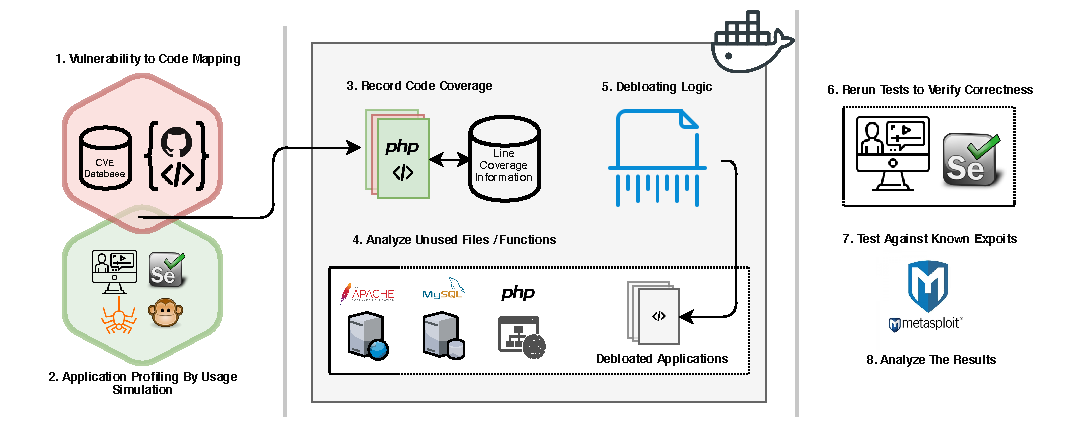
\includegraphics[width=\linewidth]{figures/lim/DebloatingPipeline.pdf}
  \vspace{-6ex}
  \caption{Overview of the architecture of our pipeline for debloating web applications and assessing the effects of different debloating strategies.}
  \vspace{-2ex}
  \label{fig:debloatingpipeline}
\end{figure*}

In this section, we briefly describe the effect of package managers on software
bloat and provide a motivating example for debloating web applications.


\subsection{Package managers and software bloat}
To ease the development of software, developers reuse third-party libraries,
external packages, and frameworks for their applications. This approach
enables developers to focus on their applications while relying on
proven and tested components. Statistics from popular package managers show
that reliance on external packages is a widely adopted practice across
many different languages. NPM, the registry hosting NodeJS packages,
reports more than 10 billion package downloads a
month~\cite{nodeDownloads}. Similarly, PyPI, the package manager for Python,
reports more than a billion a month~\cite{pypiDownloads}, while Packagist, the main repository for
Composer package manager for PHP, reports the download of 500 million
packages each month~\cite{packagistDownloads}.

At the same time, it is doubtful that \emph{all} the code and features
obtained through these packages and frameworks are actually used by
the applications that rely on them. For the most part, when developers rely on
external dependencies, they include entire packages with no effective way of
disabling and/or removing the parts of these packages and frameworks that
their applications do not require.

\subsection{Motivating web-application debloating}

In this study, we look at the bloat of web applications and quantify how
debloating can provide concrete security benefits. Even
though debloating has been successfully applied in other contexts, we argue
that the
idiosyncrasies of the web platform (e.g., the ambient authority of cookies and
the client/server model which is standard for the web but atypical
for operating systems and compiled software) require a dedicated analysis
of the applicability of debloating for web applications.

%As detailed in Section~\ref{sec:related}, several works have been
%published in the debloating domain but none of them looked specifically
%at web applications, nor did they tackle the subject from a security
%perspective. Indeed, web applications are vulnerable to different classes
%of attacks like code execution, denial of service or authentication bypass.
%Understanding the impact of debloating requires its own in-depth analysis
%that cannot be derived from other types of applications. Since we focus on
%the business logic of web applications, we decided upon PHP as the language
%used for this study. It is one of the most widely used server-side language
%in the world~\cite{phpAdoption} and very popular websites like Facebook,
%Yahoo or Wikipedia have a large part of their codebase written in this
%language. A package manager called Composer handles external dependencies
%in PHP~\cite{composer} and it relies on packages hosted on the Packagist
%website~\cite{packagist}.



To understand how the bloat of a web application can lead to a critical
vulnerability, we use a recent vulnerability of the Symfony web
framework (CVE-2018-14773~\cite{symfonyVulnerability}) as a motivating
example. Specifically, the Symfony web framework supported a legacy IIS
header that could be abused to have Symfony return a different URL than the
one in the request header, allowing the bypassing of web application firewalls
and server-side access-control mechanisms. If this type of header
was never used by the server, debloating the application would have removed
support for it, which ultimately would have prevented anyone from exploiting
the vulnerability. Drupal, a popular PHP Content Management System (CMS), was also affected by
the same vulnerability since it uses libraries from the Symfony framework
to handle parts of its internal logic~\cite{drupalVulenrability}. Even
if Drupal developers were not responsible for the code that leads to the
vulnerability, their application could still be exploited since Symfony
was an external dependency. Even more interestingly, an analysis of the
official Symfony patch on GitHub~\cite{symfonyPatch}
reveals that the vulnerable lines were derived from yet another framework
called Zend~\cite{zendVulnerability}. This shows that the structure of web
applications can be very complex with code reuse originating from many
different sources. Even if developers take all possible precautions to
minimize vulnerabilities in their own code, flaws from external dependencies
can cascade and lead to a critical entry point for an attacker.

Overall, there are clear benefits that debloating could have on web
applications. Assuming that we are able to pinpoint all the code that is required
by the users of a given software deployment, all other code (including the
code containing vulnerabilities) can be removed from that deployment.



\section{Setup}
In this section, we describe the process of gathering information regarding
known vulnerabilities (in the form of CVEs) for web applications, designing
and executing tests against web applications of interest, and identifying
the server-side code that was executed as a result of client-side actions.

\subsection{Overview}
The setup for our framework is depicted in
Figure~\ref{fig:debloatingpipeline}. To debloat target applications, we first
collect information about the vulnerabilities of the applications that we
analyze in our study. This information includes the files, functions, and
line numbers where each
vulnerability resides (Step 1, Section~\ref{sec:vulntosourcemapping}). Then,
we simulate usage of the application through a combination of different
techniques (Step 2, Section~\ref{subsec:profiling}). Using a PHP profiler
tool (\texttt{XDebug}), we record the lines, functions, and files, that are
triggered during the simulation (Step 3, Section~\ref{subsec:coverage}).

\begin{figure*}[t]
  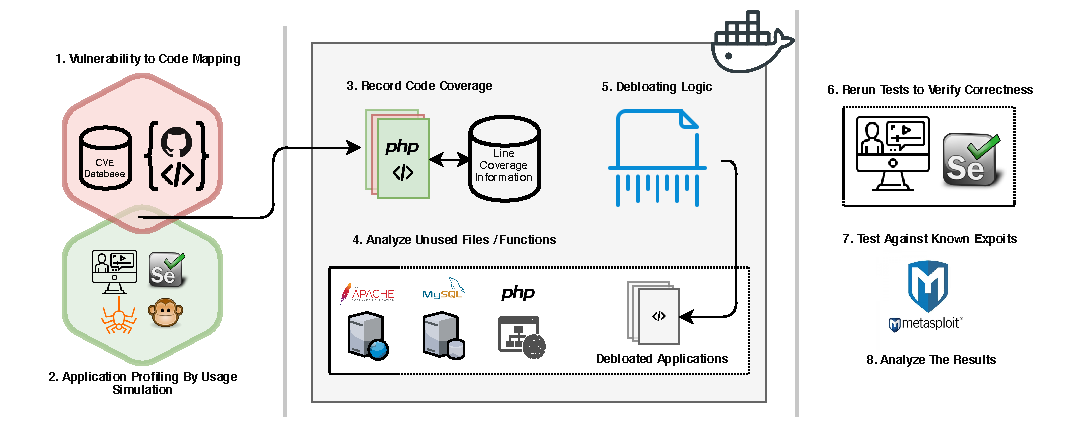
\includegraphics[width=\linewidth]{figures/lim/DebloatingPipeline.pdf}
  \caption{Overview of the architecture of our pipeline for debloating web applications and assessing the effects of different debloating strategies.}
  \label{fig:debloatingpipeline}
\end{figure*}

In the middle part of our pipeline, the debloating engine takes both the
target applications and coverage information to perform debloating at
different levels of granularity, and rewrite parts of the application to
remove unused pieces of code based on the debloating strategy being evaluated
(Steps 4 and 5, Section~\ref{sec:debloating}). Our framework also provides
a complete reporting panel to assist human analysts in understanding which
vulnerabilities can be removed by the present debloating strategies.

Last, we verify the correctness of our debloating process by running
a set of tests against the debloated web applications, and verifying that
no removed piece of code is triggered (Step 5). To this end, we
utilize assertions in place of the removed code blocks. An absence of error
messages from these assertions means that all tests were successfully
completed without triggering any missing server-side code. As a final step of
verification, we also test the debloated applications against a series of
exploits and verify that exploits which
abuse any of the vulnerabilities that were removed as part of the debloating
process, do not succeed (Step 6, Section~\ref{section:metasploit}).

To ease the integration and facilitate the analysis of new web applications, we
adopted a modular architecture that relies on three Docker containers. The
\textit{Application} container hosts our web applications.  The profiler
enabled on its web server is responsible for collecting code-coverage
information. The \textit{Database} container runs a MySQL server that
stores the code-coverage information along with the databases of the tested
applications. Lastly, the \textit{Debloating} container which includes our
debloating logic, analyzes the coverage information and generates debloated
versions of applications. It also provides a reporting panel that indicates
which vulnerabilities are removed in each application after debloating. To add
a new vulnerability, a user simply has to provide the details of the vulnerable
file(s) and line(s).

%In the end, this modular architecture makes the integration of our framework with new web applications and addition of new vulnerabilities seamless.


\subsection{Analyzed web applications}
\label{subsec:webapps}

%\begin{table*}[]
%\centering
%\caption{Analyzed open-source web applications and their corresponding versions.}
%\begin{tabular}{@{}lll@{}}
%%\toprule
%\textbf{Web Application}  & \textbf{Versions} \textit{(Release Date)}                                                                                  & \textbf{Known CVEs} \textit{($\geq$2013)}              \\ \midrule
%\multicolumn{1}{l}{Magento}                          & 1.9.0 \textsubscript{2014-5}, 2.0.5 \textsubscript{2016-4}                                                                             & 10                       \\ \midrule
%\multicolumn{1}{l}{MediaWiki}  & \multicolumn{1}{l}{1.19.1 \textsubscript{2012-06}, 1.21.1 \textsubscript{2013-05}, 1.23.0 \textsubscript{2014-06}, 1.24.0 \textsubscript{2014-11}, 1.28.0 \textsubscript{2016-11}} & \multicolumn{1}{l}{111} \\ \midrule
%\multicolumn{1}{l}{phpMyAdmin} & \multicolumn{1}{l}{4.0.0 \textsubscript{2013-05}, 4.4.0 \textsubscript{2015-04}, 4.6.0 \textsubscript{2016-03}, 4.7.0 \textsubscript{2017-03}}                      & \multicolumn{1}{l}{130} \\ \midrule
%\multicolumn{1}{l}{{Wordpress}}                          & {3.9.0 \textsubscript{2014-4}, 4.0 \textsubscript{2014-9}, 4.2.3 \textsubscript{2015-7}, 4.6 \textsubscript{2016-8}, 4.7 \textsubscript{2016-12}, 4.7.1 \textsubscript{2017-1}}                                                                             & {131}                       \\
%\bottomrule
%\end{tabular}
%\label{table:analyzed_webapps}
%\end{table*}

To understand how the process of debloating increases the security of web
applications, we decided against using toy-like web applications. Instead,
we focused on established open-source applications with millions of users,
and the presence of a sufficient number of known historical vulnerabilities
(in the form of CVEs) to allow us to generalize from them. To this end, we
selected {phpMyAdmin}~\cite{phpmyadmin},
{MediaWiki}~\cite{mediawiki}, {Magento}~\cite{magento}, and WordPress~\cite{wordpress},
which are representative samples of four different types of
web applications namely web-administration tools, wikis, online
shops, and blogging software. Table~\ref{table:analyzed_webapps} shows the versions of these web
applications that we utilized, in order to map CVEs to the location of the
vulnerability in the source code of each application.


%Initially, we study the registered CVEs for a subset of famous open source
%PHP applications. To capture different types of application architectures, we
%cover the following range of categories: \textit{``Web Administration Tools''}
%with phpMyAdmin, \textit{``Wiki''} with MediaWiki and \textit{``Online
%Shops''} with Magento. To map registered CVEs to the vulnerable piece
%of source code for each application, we used a set of versions for each
%application that contain the studied CVEs. These applications are listed
%in Table~\ref{table:analyzed_webapps}.
% We can refer to buildwith stats if we need to reason about why we chose these applications, both usage statistics and registered covers
% Why PHP: https://trends.builtwith.com/framework/programming-language
% Ecommerce: https://trends.builtwith.com/shop

\begin{table}[]
\centering
\caption{Analyzed open-source web applications.}
\scalebox{0.87}{
\begin{tabular}{|l|l|c|}
\hline
\textbf{Web Application} & \textbf{Version}                            & \begin{tabular}[c]{@{}l@{}}\textbf{Known CVEs}\\\hspace{1em}(2013-2019)\end{tabular} \\ \hline
Magento                  & 1.9.0, 2.0.5                                 & 10                                                                     \\ \hline
MediaWiki                & 1.19.1, 1.21.1, 1.24.0, 1.28.0 & 111                                                                    \\ \hline
phpMyAdmin               & 4.0.0, 4.4.0, 4.6.0, 4.7.0     & 130                                                                    \\ \hline
WordPress                & 3.9.0, 4.0, 4.2.3, 4.6, 4.7, 4.7.1  & 131                                                                    \\ \hline
\end{tabular}
}
\label{table:analyzed_webapps}
\end{table}

\subsection{Vulnerability to source-code mapping}
\label{sec:vulntosourcemapping}
To determine whether debloating web applications can actually remove
vulnerabilities, we performed a mapping of known CVEs to the vulnerable lines,
functions, and files, that they exploit in each application. This way, by
looking at an application after debloating, we can determine if the files,
functions, or lines responsible for the vulnerability, are still present or
were removed during the debloating process.


Even though there exist multiple databases listing the current and
historical CVEs of popular software (including the web applications in
question)~\cite{cvedetails,nistgov}, locating the actual source code
containing the vulnerability described in a CVE, is a non-trivial process
which requires careful investigation. In some cases, the right patch can be
discovered because of a direct reference to a CVE in a commit message, or in
a bug report on official public repositories of web applications. For others,
the fix is included within numerous commits that have to be carefully analyzed
to locate the appropriate lines of code. Since a vulnerability can span over
multiple lines, functions, and even multiple files, we record all affected
locations in a database so that this information can be later correlated
with each evaluated application.

%\todo{The following paragraph seems out of place... perhaps something for
%the background section}
%The premise behind debloating is that vulnerabilities exist in parts of a
%program that are never used in specific deployments of interest, and therefore
%can be safely removed (i.e., debloated). This makes the success of debloating
%highly dependent on the usage profile of an application and the location of
%any given vulnerability.
%%In the end, as debloating is based on specific usage profile, some
%%vulnerabilities may be more frequently mitigated than others depending on their
%%location in the source code. If a vulnerability belongs to a feature within
%%the application that is rarely triggered by normal users or that is hidden
%%behind privileged access, they may often be removed from the source code.
%To understand this better, we cam investigate a specific example of critical
%vulnerability. CVE-2016-6620 is a PHP object injection vulnerability that
%affects phpMyAdmin 4.6.0. It has a CVSS score of 9.8 which represents a highly
%severe and critical vulnerability inside phpMyAdmin. It consists of calling
%the PHP \textit{unserialize} function with unsanitized user-supplied data
%which then leads to code execution upon deserialization. This vulnerable
%feature has to be manually enabled by the user and is not part of the
%default configuration of phpMyAdmin. Hence, most usage profiles from real
%users will likely not contain any calls to this PHP \textit{unserialize}
%function, allowing the vulnerable code to be safely removed.


Given the time-consuming nature of mapping CVEs to existing code, for
this study, we limited ourselves to, at most, 20 CVEs per application
of interest.
The complete list of CVEs we mapped for this study can be found in
Table~\ref{table:listofallcves} in the Appendix.
To select these CVEs, we ordered existing vulnerabilities by
their CVSS score (thereby selecting the ones that are the most critical)
and we did not consider vulnerabilities that were reported before 2013. This
focus on fairly recent vulnerabilities (i.e., in the last five years) makes
our results more generalizable to the current state of web applications,
as opposed to quantifying vulnerabilities in source-code which has since
dramatically evolved. Note that, because not all versions of a web application
are vulnerable to all evaluated CVEs, we had to map vulnerabilities
across a number of different versions, as shown in
Table~\ref{table:analyzed_webapps}.



\subsection{Application usage profiling}
\label{subsec:profiling}

Modern web applications provide an incredibly wide range of features and
options to their users. Even though, from a functional perspective, more
features are desirable, from a security perspective, the code that implements
new features may contain new vulnerabilities thereby further expanding
a program's attack-surface. In order for a system to be
able to remove code related to unnecessary features, one must first identify
which features are necessary for a target set of users.

Given a usage profile, the goal of our framework is to produce debloated
versions of web applications which maintain the code and features that are
part of that profile but remove the rest. To be as objective as possible with
what features are considered ``necessary,'' we utilize four independent
sources of web application usage: i) online tutorials describing how to use
the applications of interest, ii) web crawlers that autonomously navigate
the application, iii) vulnerability scanners that feed malicious content to the
application, and iv) monkey testing tools that click on random parts of webpages
and type random keystrokes. The combination of all four gives our profiles
both breadth (through the crawler and monkey testing) as well as depth (through
the user following complicated paths while providing expected inputs and the
vulnerability scanner which provides large amounts of malicious inputs trying
to exploit the web application).

%In order to test our pipeline for this study, we created our own usage profile from scratch by using a combination of different automated techniques.
%First, to cover the core features of our tested web applications, we followed online tutorials and wrote Selenium tests based on them.
%This way, we obtain replayable tests that trigger the most essential lines in an application.
%Then, to augment coverage and add easy-to-reach options that are likely to be triggered, we used two additional techniques: spider software that can crawl the pages of the application interface and submit forms, and monkey testing scripts that click on random locations on the screen and type random keystrokes.
%While following the tutorials covers key functionalities within the application, monkey and spider tests add more breadth to our coverage.


%Different users use different parts of web applications, this can be a result of an access restriction model or be based on the need of different users. Specialized applications will have their unique usage profile as studied by [cite the paper that studies usage profile of industry application]. In our model, we simulate a general user that installs the application and uses available online tutorials to find his way through the applications. To that end, we automated the tutorials for our target web applications using selenium, to augment the coverage and add easy to reach options that the users are likely to trigger, we used spider software that would crawl the pages of the website and submit forms in addition to a monkey testing script that would click on random locations on the screen and type random keystrokes. While following the tutorials covers deep functionalities within the application, monkey and spider tests add more breadth to our coverage.

\subsubsection{Tutorials}
\label{sec:tutorials}
To simulate common interactions with an application, we use a popular search
engine to search for the application's name followed by the word ``tutorials''
(e.g., ``phpMyAdmin tutorials'') and follow the tutorials from the first two
pages of search results.

Specifically, we map each tutorial to a Selenium script that allows us to
both execute the same tutorial multiple times and also assess the correctness
of the results (e.g., encode that when we delete a database using phpMyAdmin,
the deleted database is no-longer shown in the list of databases). Note that
this mapping of tutorials to Selenium scripts is yet another time-consuming
process which, occasionally, has to be repeated for different versions of
the same web application. One change in a form field or in a selector can
break the complete flow of a test suite, and we observed a significant number
of cases with slight interface changes between two consecutive versions of
the same application.

Overall, after fine-tuning the scripts for all our tested versions, we obtained
46 tutorials which translated into 302 use cases scripted as Selenium tests
requiring 16,025 lines of code. Given our desire for complete reproducibility
of our results, we include the complete list of tutorials in the Appendix
(Table~\ref{table:listoftutorials}) along with WebArchive links that will
remain available despite potential future domain expirations and linkrot of
the original URLs~\cite{koehler2004longitudinal}.

%Tutorials model the behavior of the vast majority of users who try
%to setup the minimum necessary functionalities of applications and start
%working with them.
%While this approach triggers benign and valid use cases of the applications, it
%does not run code paths that lead to invalid inputs and does not cover the code
%for error handling.

Below, we provide a non-exhaustive list of actions that were part of the followed tutorials of each web application. 
% Full details are available in the actual tutorials and in the Selenium scripts which we will release together with this paper.
\vspace{0.5ex}

\noindent \textbf{Actions covered by phpMyAdmin tutorials:} As a web administration tool, all phpMyAdmin functionality is protected by an authentication mechanism.
We followed the actions described by tutorials when logged in as a root user account with full application access. The Selenium-encoded tutorials cover database operations including creating and dropping databases, filling tables with data, querying, table indexes, and importing/exporting data.
They also include administration tasks such as adding new user accounts, optimizing databases, checking database server status, obtaining performance metrics, and accessing server settings such as variables, charsets, and engines.

\vspace{0.5ex}

\noindent \textbf{Actions covered by MediaWiki tutorials:} MediaWiki provides different features depending on the privileges of the user.
Unauthenticated users can only visit and search pages.
Registered ones can post and edit content while administrators can perform moderation and management operations.
The tutorials that we followed cover all these different use cases.
More specifically, actions coded in our tutorials include authentication, creating and renaming pages, importing and exporting content from the wiki, as well as changing settings such as skins, styles, and formatting options.
%Modifying the navigation menu is a task that can only be performed by an administrator and is also covered by the tutorials. Finally, the tutorials also cover the importing and exporting content from the wiki.

\vspace{0.5ex}

\noindent \textbf{Actions covered by WordPress tutorials:} As a blogging software, WordPress has two distinct entry points, one for normal unauthenticated users to read blogs and post comments, and a separate administration panel accessible to privileged and authenticated users.
WordPress tutorials mostly focus on administrative tasks since normal users have limited abilities. The Selenium-encoded tutorials include actions such as creating a new post using HTML for the content, modifying most post options (ranging from visibility and tags to setting featured images), as well as downloading and changing WordPress themes.
%They cover different settings and include the managing of categories and tags.
For the administration panel, the tutorials include exporting content, setting up user accounts, and uploading media. Finally, the tutorials include the visiting of posts and the posting of comments as well as the management of comments, such as approving them, marking them as spam, and deleting them.
\vspace{0.5ex}

\noindent \textbf{Actions covered by Magento tutorials:} Magento is the largest evaluated web application in terms of source code and has the most features compared to the other applications. Similar to WordPress, the tutorials mostly target administration tasks which include store settings, advanced product search options, order notification via RSS, product pricing, currencies and tax rules, delivery and payment methods, emails and notifications, reviews and ratings and cache control. Some tutorials go in even more details by covering product and stock management, managing customers and groups configurations, modifying the UI, creating pages, and using widgets.
On the customer side, we followed tutorials that included registration of a new account, authentication actions, and purchasing products until checkout.






\subsubsection{Monkey testing}
\label{sec:monkey}
Monkey testing is a method for testing
software where the simulated user sends random clicks and keystrokes to the
target application. This unpredictable behavior can uncover bugs in an
application as it can trigger paths and actions that were not anticipated by
developers. In our case, we use such a technique to trigger additional code,
not covered by tutorials. We observe that this approach adds breadth to the
code-coverage by reaching easy to access features. In addition, by feeding
random keystrokes into forms, monkey testing can bring the application in an
error state thus exercising error-handling pieces of code.

We rely on the stress-testing library called
\texttt{gremlins.js}~\cite{gremlinsjs} in conjunction with the GreaseMonkey
browser extension~\cite{greasemonkey} to inject the library into web
application pages.
%During pilot stages of these experiments, we experimented
%with different configurations for \texttt{gremlins.js} (in terms of its
%combinations of Click, Scroll, Keystroke, and Delays actions) and arrived
%at a configuration that exercised as much as possible of each tested web
%application.
Since this kind of testing can occasionally trigger unwanted actions, we have
to take necessary steps to stop them, e.g., prevent the test from leaving
the web application and visiting external websites. We also want to prevent
\texttt{gremlins.js} from getting trapped on a single page as an unexpected
JavaScript
%\texttt{alert} or \texttt{prompt}
dialogue box or a dead end page can pause our test
execution.  %or the monkey can get stuck on a deadend page.
An additional issue is that of accidentally logging out a web application by
clicking on a logout link. Given that we run monkey-testing under three different
usage profiles (public user, logged-in user, and administrator) we took steps
to avoid accidental logouts. Overall, we perform the following
modifications: i) we remove all links that lead to external pages, ii) we
remove logout buttons for applications that require authentication, iii) we
override the aforementioned JavaScript functions and iv) we set a timeout to
detect when the monkey is stuck and reset it to a known good state. All these
actions are done using injected JavaScript on target pages prior to starting
the \texttt{gremlins.js} library.

To cover a large set of pages from a web application, we run
\texttt{gremlins.js} for 12 hours for each of the test profiles.
To guarantee the reproducibility of our experiment, we choose a fixed seed for
each run that will generate the same sequence of pseudo-random actions.


\subsubsection{Crawling}
Web spiders (also known as crawlers) are a type of bot that follows the
links of a web application and optionally submits forms with predefined
content. Each newly crawled page is added to a database of the application that
the crawler uses to prevent repeated visits to the same pages. For our study,
we use BurpSuite Spider v2.0.14~\cite{burpsuite} to crawl our web
applications. As a result, we augment the application coverage with code paths that were
not triggered, either through the followed tutorials or through monkey testing.

%Our results show that monkey testing and spiders produce different code-coverage and trigger different functionalities within tested applications. Hence, these two methods help us increase the diversity of our usage profiles.
%Hence, this is necessary to include both of these tests.

\subsubsection{Running vulnerability scanners}
Vulnerability scanners are tools that try to detect security flaws in web applications.
%In our case, the scanner increases our code-coverage by reaching unwanted states in the application.
We use BurpSuite Scanner v2.0.14~\cite{burpsuite} based on the URLs extracted by the spider to look for vulnerabilities in headers, URLs and forms.
Notably, the scanner tries different injection mechanisms like SQL injection, XSS, PHP file injection, and path traversal, to trigger errors and reach unwanted states in the application.
The vulnerability scanner goes beyond what the crawler and the monkey cover by modifying headers and URL parameters.
By inspecting the resulting coverage, we observe that each of these four methods result in exercising server-side code that would not have been exercised through the other methods. We quantify this relationship in Section~\ref{section:results}.


\subsection{Recording server-side code-coverage}
\label{subsec:coverage}

Regardless of the method that is used to interact with a web application,
in order to be able to successfully remove unused code (i.e., debloat the web
application), we must be able to
associate client-side requests with server-side code. To record the files
and lines of code that are triggered by user requests, we make use of PHP
profilers.

PHP profilers are available as PHP extensions that modify the PHP engine to
collect code-coverage information. There exist a number of different profilers,
such as, \texttt{XDebug}~\cite{XDebug}, \texttt{phpdbg}~\cite{phpdbg}, and
\texttt{xhprof}~\cite{xhprof} all of which require a similar setup to record
code-coverage. For our framework, we decided to use \texttt{XDebug} as it
is the most mature profiler and is actively maintained.

\subsubsection{Adding coverage support in a web application}

\vspace{1ex}
\noindent\textbf{Connecting a web application to XDebug.}
To be able to perform dynamic analysis and record lines of code
that are triggered by user requests, our framework must add calls
to specific \texttt{XDebug} functions in every PHP file of a web
application. Specifically, both \texttt{xdebug\_start\_code\_coverage()} and
\texttt{xdebug\_get\_code\_coverage()} functions are called to, respectively,
start and receive coverage information. If the ``get'' function is never
called, the coverage information is lost. In the following paragraphs, we
describe challenges related to obtaining the code-coverage from \texttt{XDebug}
and how we overcame them.

\vspace{1ex}
\noindent\textbf{The case of unrecorded lines.}
Boomsma and Gross reported on the possibility of removing unused code in a
custom PHP application~\cite{boomsma2012Dead}. By performing dynamic
analysis, they observed which files were not used and removed
them from their application. The authors utilized their own profiler and took
advantage of the \texttt{auto\_append} built-in function of PHP to add
the necessary log functions at the very end of all PHP files~\cite{autoappend}.

For our study, we initially attempted to use the same approach and ran
preliminary tests by appending \texttt{XDebug} function calls at the end
of our tested files. However, we discovered that the coverage was
incomplete and that some lines were not properly recorded. Given that any
PHP file can call the \textit{exit()} or \textit{die()} function at any
time to terminate the current script, our \texttt{XDebug} calls which were
located at the end of each file, were not always executed thus leading to
under-reported code-coverage.


%Since our ``xdebug\_get\_code\_coverage()'' calls were located at the very
%end of each PHP file, we were not able in some cases to collect the full
%coverage information because of these exit calls. For us to properly debloat
%our target web applications, we needed to go further.


\subsubsection{Main challenges for getting full coverage}
\label{subsubsec:challenges}

\vspace{1ex}
\noindent\textbf{Avoiding early exits.}
To overcome the coverage problems due to calls to exit functions, we
utilized a specific type of PHP callback functions, called \textit{shutdown}
functions. When registered, these functions are triggered after all the
code on the page has finished running or after either \textit{exit()} or
\textit{die()} functions are called. This way, we are able to obtain the
desired coverage information even if a PHP script used one of the aforementioned functions.
Interestingly, we also discovered that calls to \textit{exit()} inside a
shutdown function prevent the execution of other shutdown functions
including the call to collect our own code-coverage information. To correct
this issue, we statically analyzed the evaluated applications and automatically
added calls to collect code-coverage before these exit calls (e.g., Line 7
in Listing~\ref{listing:rewriting_webapps}).

\vspace{1ex}
\noindent\textbf{Getting correct coverage information of shutdown functions.}
Another challenge, in terms of recording correct code-coverage information,
is to properly record the executed lines of code inside shutdown functions. As
mentioned by the PHP manual~\cite{phpshutdown}, shutdown functions are called
in the order they were registered. This means that if our own shutdown function
is registered first, it will also be triggered first, thereby missing any
calls to subsequent shutdown functions present in the same PHP file. To get
full coverage, we use the following approach: our own shutdown function will
perform a late registration of a final shutdown function that will be added
at the very end of the execution queue. This way, we can be certain that
the very last shutdown function that will be executed in a script will be
our own, providing us with the desired coverage information.


\vspace{1ex}
\noindent\textbf{Getting correct coverage information of destructors.}
The final challenge that we faced was to properly record covered lines for
all class destructors. PHP uses garbage collection and reference counting to
remove objects from memory, whenever they are no longer necessary. However,
there is no real way to anticipate when the garbage collector will effectively
remove objects during program execution. If objects are destroyed \emph{before}
the shutdown functions are executed, our framework has no issue recording
them. However, if they are destroyed after, our shutdown functions are
incapable of registering the execution of these destructors.

To handle this special case, we rewrote class destructors so that they
register themselves while they are executing. Every time a destructor
is called, we query the \texttt{XDebug} engine to check whether code-coverage
recording is currently in progress. This way, we can determine whether the
destructor is called before or after shutdown functions. If the destructor
is called after shutdown functions, we dynamically decide to start recording
all executed lines within the destructor and save the coverage information
when it finishes executing.

%Every time a destructor is called, we query the XDebug engine to know if it was registered before.
%If it was not, we start recording all executed lines and save the coverage information when it finishes executing.

\begin{figure}[t]
  \begin{lstlisting}[frame=single, caption={Code rewritten by the debloating framework to ensure correct code-coverage of corner cases.},captionpos=b, label={listing:rewriting_webapps}]
  <?php
  register_shutdown_function("PMA_Response::resp");
  class PMA_Response {
    public static function resp() {
      $buffer->flush();
      // Prepend original call to exit:
      collect_code_coverage();
      exit;
    }
  }
  
  class TCPDF {
    public function __destruct() {
      // If called after shutdown_functions
      // start recording code-coverage
      ...
      // If called after shutdown_functions
      // stop coverage
    }
  }
  ?>
  \end{lstlisting}
\end{figure}

\vspace{1ex}
\noindent\textbf{Summary.}
%We use prepend and register shutdown functions
%we prepend before exit lines call to get coverage
As witnessed through the above use cases, collecting the correct code-coverage information
for a web application is significantly more complicated than one would
initially expect. Through the preprocessing of code, and the use of destructors
and shutdown functions, we solve the issues that were not even mentioned
in prior work and get a precise view of the code that executes at the server
side, as a result of user requests. Listing~\ref{listing:rewriting_webapps}
provides an example of concrete modifications in a PHP file. On line 7, we
added a code-coverage call before an \texttt{exit} which happens inside a shutdown functions to prevent information
loss due to early exits. On lines 14 and 17, we wrapped the destructor with
code-coverage calls.


%*****************************OLD
%\paragraph{Gathering coverage information when all PHP code has finished executing}
%In PHP, developers can register functions as ``shutdown\_functions'' that would be triggered by PHP engine after all the code on the page has finished running or after either \textit{exit()} or \textit{die()} functions are called.
%Our framework uses the same method to make sure ``xdebug\_get\_code\_coverage()'' is executed last.
%As described in the PHP language manual, if multiple shutdown\_functions are present, they will be executed in the same order that they are registered.
%
%At the same time, PHP scripts can call \textit{exit()} at any time during the execution.
%Architectures that use auto\_append to collect coverage information will miss the coverage for scripts that call \textit{exit()}.
%More interestingly, if this call to \textit{exit()} happens inside a shutdown\_function(), it will prevent the execution of other shutdown\_functions including the call to collect code-coverage information.
%
%\paragraph{code-coverage for PHP destructors} is another challenge that we have to overcome, PHP uses garbage collection and reference counting to remove objects from the memory. We can not reason about the exact time when destructors get executed. PHP object destruction order will call zend\_call\_destructors which then calls destructor functions of the remaining objects after shutdown\_functions are called.
%
%
%
%\subsubsection{Preparing web applications}
%\label{label:prep_software}
%Our framework statically analyzes web applications and rewrites their code to conform to our testing requirements mentioned in section~\ref{subsec:coverage}. Our three step solution to address issues mentioned in Section~\ref{subsec:coverage} uses a combination of preprocessing and programming hacks as depicted in Listing~\ref{listing:rewriting_webapps}.
%
%To make sure our call to collect the code-coverage is always executed, we statically analyze the applications and automatically prepend calls to \textit{exit()} with a call to collect code-coverage (Line 7). This way we make sure we have full coverage information before exiting and also do not change the original execution flow of applications.
%
%The second step is necessary to guarantee that our shutdown\_function which collects code-coverage information runs last. To achieve this, we register a second shutdown\_function within the first shutdown\_function and this trick makes sure the second registered function runs after all previously registered shutdown\_functions.
%
%Third step is to record code-coverage for all class destructors. We distinguish between two cases, destructors may execute before we stop recording code-coverage (i.e, before shutdown\_functions are called). In this case we do not need to do anything extra. But when destructors execute after after shutdown\_functions, we modify them to start recording code-coverage information and save this data after they finish executing. We track this state by querying XDebug engine to see if coverage recording is currently in progress and distinguish between the two cases. To handle this situation, our framework rewrites class destructors to call XDebug functions to record their coverage (Line 15 and 18 in Listing~\ref{listing:rewriting_webapps}).
%
%%One requirement is to make sure our function that collects code-coverage runs last, to do that we use shutdown\_functions. To prevent calls to \textit{die} or \textit{exit} before our shutdown\_function preventing its execution, our %framework preprocesses target web applications and rewrites such calls to make sure our shutdown\_function executes. Second requirement is to record code-coverage for destructors that run after shutdown\_functions, to that end the %framework rewrites destructors with proper calls to XDebug code-coverage functions.
%

\section{Debloating web applications}
\label{sec:debloating}

In this section, we briefly describe the evaluated debloating strategies and
the steps we took to ensure that the debloated applications remain functional.


\subsection{Debloating strategies}

By combining the simulated usage of a web application (achieved through
tutorials encoded in Selenium scripts, web crawlers, monkey testing, and
vulnerability scanning) with
server-side code profiling, we can identify the code that was executed
as part of handling web requests. Consequently, code whose execution was
not triggered by any client-side request can presumably be removed since
it is not necessary for any of the functionality that is desired by users
(as quantified by the utilized usage profiles).
In this work, we evaluate the following debloating strategies:
\vspace{-2ex}
\paragraph{$\bullet$ File-level debloating:} Given that the source code of web
applications spans tens or hundreds of different files, we can completely
remove a file, when none of the lines of code in that file were executed
during the stimulation of the web application.
\vspace{-2ex}
\paragraph{$\bullet$ Function-level debloating:} In function-level debloating, not
only can we remove entire files, but we can also selectively remove some of
the functions contained in other files. This is a more fine-grained approach
which allows us to remove more code, than the more conservative, file-level
debloating strategy.

%\begin{itemize}
%  \setlength\itemsep{0.5em}
%\item \textbf{File-level debloating:} Given that the source code of web
%applications spans tens or hundreds of different files, we can completely
%remove a file, when none of the lines of code in that file were executed
%during the stimulation of the web application.
%
%\item \textbf{Function-level debloating:} In function-level debloating, not
%only can we remove entire files but we can also selectively remove some of
%the functions contained in other files. This is a more fine-grained approach
%which allows us to remove more code, than the more conservative, file-level
%debloating strategy.
%\end{itemize}

More fine-grained approaches are possible, such as, the removal of specific code statements from retained functions which were not exercised during stimulation.
However, such changes essentially modify the logic of a function (e.g., removing
conditional code blocks) thereby increasing the probability of breaking the
resulting program when a minute change of a client-side request would lead the
execution into these blocks of code.
%{\color{blue} Moreover, recording the coverage of error handlers is a challenge that sub-function debloating mechanisms have to address. Error states that are not triggered during profiling will lead to the removal of such conditions and the final application will lack proper error handling upon receiving previously unseen requests.
%During the development of web applications, usually a function (e.g., a controller action in MVC architecture or its equivalent) contains the complete logic to handle the request. This standard architecture adopted by most web development frameworks relies on central error handling classes.
%This includes the code to handle proper execution of the function in addition to the code to handle errors. Even though this logic can be separated into different functions and classes,
%the decision to keep or remove the function does not break this chain.
%As such, we consider this level of debloating as out of scope, and leave its evaluation for future work.}


\subsection{Detecting the execution of removed code}


We replace all removed functions and files with placeholders which, if executed,
have the following tasks:
\vspace{-2ex}
\paragraph{$\bullet$ Exit the application:} If a placeholder happens to be triggered,
the PHP application will start its shutdown procedures. This way, the
application does not enter an unexpected state that was not planned by the
debloating process.
\vspace{-2ex}
\paragraph{$\bullet$ Record information about the missing function:} In order
to better understand which missing placeholders were triggered and how,
our framework logs several pieces of information, such as, the URL that
triggered the execution of the removed code, the name of the class and
function of the removed code, and the
corresponding line numbers.

%\begin{itemize}
%  \setlength\itemsep{0.5em}
%\item \textbf{Exit the application:} If a placeholder happens to be triggered,
%the PHP application will start its shutdown procedures. This way, the
%application does not enter an unexpected state that was not planned by the
%debloating process.
%
%\item \textbf{Record information about the missing function:} In order
%to better understand which missing placeholders were triggered and how,
%our framework logs several pieces of information, such as, the URL that
%triggered the execution of the removed code, the name of the class and
%function of the removed code, and the
%corresponding line numbers.

%{\color{red}TODO:\item \textbf{Proactively preventing required code from being removed:} Certain actions within web applications are not triggered by users and %sometimes specific actions need to run at certain intervals. Regardless of
%the entity triggering the action, our system is able to record its coverage. But if the interval to run the action is longer than the interval that record the code %coverage is recorded, the underlying code for that feature will be removed.

%**I'm not sure into how much detail I want to go here, shall I open the can of worms and talk about update scripts? We haven't spend that much time discovering and %whitelisting these stuff.
%The main goal here is to introduce whitelisting for error handlers, config files and the files that we know we do not use often but they are still required.**
%}
%\end{itemize}

To ensure that the debloating process has preserved the functionality of
the debloated web application, we rerun all the Selenium-mapped tutorials and monkey scripts
after the debloating stage. If our placeholder code for removed files and
functions executes during this stage, this means that this code should not
have been removed.

This feedback mechanism proved invaluable during the development of
our framework since it helped us identify problems with our coverage
logic which in turn revealed the challenges that we described in
Section~\ref{subsubsec:challenges}.

%%%%%%%%%%%%%%%%%%%%%%%%%%%%%%%%%%%%%%%%%%%%%%%%%%%%%%

%\paragraph{Assertions} are used throughout our debloating logic, when we debloat a unit of code, we replace it with a placeholder that contains an assertion code. If debloated files or functions are triggered, this code will notify us via web server logs that one of the tests triggered a removed unit of code along with useful information such as referer header, the page which triggered the execution of removed code and class name, function name and line number of the removed piece of code. This information is then used to verify the correctness of our debloating when rerunning tests in verification step.
%
%To prevent unwanted side effects when executing web applications after debloating, these assertions and placeholders stop the code execution to prevent execution of code paths which include removed functions and files.


%%%%%%%%%%%% TO BE PUT IN THE RESULTS SECTION
%\subsection{Definition of vulnerability coverage}
%An exploitable vulnerability in a web application can be the result of multiple vulnerable lines, functions or files that together they create a chain that leads to an exploit. On one end an application developer might fail to apply sanitization function on untrusted input which affects only one line of code but the same bad practice can be spread over multiple files, on the other end a chain of vulnerabilities has to be present and be chained together to form an exploit for a registered CVE.
%
%For each vulnerability, when our usage profiles line coverage data overlaps with vulnerable lines, we call the vulnerability to be triggered by our usage profiles regardless of full or partial overlap. In that sense we take the conservative approach.
%
%An executable line within a PHP application is considered triggered if usage profiles execute that line. Similarly a function is considered to be covered if usage profiles execute the first executable line within that function. This definition is based on the logic of PHP compiler and Zend engine where we do not have a notion of functions directly and have to define functions as the line number of first executable statement within them. One the same note, we define a PHP file to be covered by usage profiles if at least one executable line within that file is triggered. Based on these definitions we propose debloating methods that can remove units of code not triggered by usage profiles.


%\subsection{Debloating strategies}
%Based on usage profile information, we define a baseline debloating method which only removes PHP files if non of the executable lines within those files are triggered. We also analyze the potential benefits from debloating strategies which can remove specific vulnerable lines within the web applications if the usage profiles do not cover those lines. All other debloating methods should perform between these bounds in terms of mitigated CVEs. Second debloating strategy we introduce debloats functions. Our experiments show that this strategy works just as good as more fine grained debloating strategies in terms of removed CVEs. Note that while previous usage profiles might show that users do not trigger specific units of code through normal usage, attackers can still trigger the code. Hence, the debloated code should handle this situation properly, this challenge makes fine grained debloating that modified individual executable lines more challenging. Table~\ref{table:debloating_bounds} shows the performance of debloating strategies on the analyzed web applications in terms of removed CVEs.
%
%\begin{table}[]
%\begin{tabular}{|l|l|l|l|}
%\hline
%Web Application & \begin{tabular}[c]{@{}l@{}}Total\\ CVEs\end{tabular} & \begin{tabular}[c]{@{}l@{}}Lowerbound/\\ Upperbound\end{tabular} & \begin{tabular}[c]{@{}l@{}}Function\\ Debloating\end{tabular} \\ \hline
%phpMyAdmin      & 20                                                   & 7/15                                                             & 13                                                            \\ \hline
%MediaWiki       & 21                                                   & 6/13?                                                            & 15                                                            \\ \hline
%Magento         & 8                                                    & x/x                                                              & x                                                             \\ \hline
%\end{tabular}
%\caption{Debloating performance bounds}
%\label{table:debloating_bounds}
%\end{table}
%
%
%\subsection{File level debloating}
%The baseline debloating strategy we discuss debloats PHP files that are not covered by usage profiles. On average this approach yields removal of UPDATE**\%25** of known CVEs and reduces code size by **Y** amount. This approach is the least aggressive approach with limited effectiveness.
%\subsection{Function level debloating}
%In this approach, our framework removes functions that are not covered by our usage profiles and replaces them with assertions. Our analysis proves this approach to have a performance close to the upper bound of debloating strategies (i.e, a debloating strategy that debloats individual lines) in terms of number of removed CVEs. While the side effects of removing functions are minimal compared to individual lines, the result turns out to be promising. As shown in Table~\ref{table:debloating_bounds}, function level debloating on average mitigates **UPDATE NUMBER** \%75 of known CVEs on target web applications.

\section{Results}
\label{section:results}

To assess the impact of debloating web applications, we analyze our results
from a number of different perspectives. First, we show the contributions of different application-profiling methods and then compute different metrics
to understand the effectiveness of debloating in terms of reducing the attack surface of our tested applications. Next, we focus on CVEs to determine whether
debloating can actually remove critical vulnerabilities. Then, we take
a closer look at the bloat introduced by external packages along with the
security implications that come with using this specific development practice.
Finally, we look at what has effectively been removed in debloated applications and test a number of exploits against the original and debloated versions of the evaluated web applications.
% we use clustering to find which parts of the application are more affected by debloating.


%Property Oriented Programing (POP) is an exploitation technique in PHP which works similar to ROP (Return Oriented %Programming) and is used to exploit POI vulnerabilities. In this technique, the attacker creates exploit gadgets from %available code in the applications. Each object within the chain performs malicious actions or prepares the environment for %execution of next object in the chain upon deserialization. Dahse et al. have studied automatic generation of such gadget %chains in \cite{Dahse:2014:CRA:2660267.2660363}.

\subsection{Tutorials vs. Monkey Testing vs. \\Crawling vs. Vulnerability Scanning}
As described in Section~\ref{subsec:profiling}, to ensure that we exercise web applications in an objective and repeatable way, we utilized tutorials, monkey testing, crawlers, and vulnerability scanners. Figure~\ref{fig:venncoverage} shows the coverage, in terms of server-side files, that each method obtained on the latest version of each web application in our testbed. We can clearly see that all four methods are required, with each method contributing differently for different web applications.
For example, tutorials trigger more files in Magento compared to other applications, while Spider covers most unique files in WordPress.

%For example, while monkey testing appears to be responsible for triggering the vast majority of source code in MediaWiki, it does not perform nearly as well for the %remaining two applications.

\subsection{Debloating by the numbers}
To evaluate the effectiveness of our two debloating strategies, we computed different metrics that provide
insights into what has actually been removed during the debloating process.


\subsubsection{Logical lines of code}
\label{subsubsec:lloc}
The size of a program positively correlates with the number of programming errors (i.e., bugs). According to McConnel~\cite{mcconnell2004code}, the industry average, at least in 2004, was to have between 1 and 25 bugs for every one thousands lines of code. Given the importance of the size of an application to its overall security, we start by estimating the reduction of the attack surface by looking at the
Logical Lines Of Code (LLOC, sometimes also called Effective Lines Of
Code). LLOC is intended to measure lines of code without comments, empty
lines and syntactic structure required by the programming language. LLOC
reduction is a robust and precise indicator of how much the volume of
the code was reduced.
Figure~\ref{fig:lloc} reports on the LLOC for all versions of the applications
we debloated.

\paragraph{Number of logical lines over time.}
Looking at the number of LLOC of the original applications, we can observe two different evolution behaviors.
For WordPress, the amount of code is stable and there is even a small decrease of 2\% of LLOC between versions 4.7 and 4.7.1.
For the other applications, we observe the opposite where the source code in the latest versions spikes, compared to the ones released just before them: 82\% LLOC increase for phpMyAdmin, 99\% for MediaWiki, and 171\% for Magento. By
analyzing the code of these newer versions in an attempt to understand their
sudden expansion in size, we discovered that these spikes can be attributed to
a change in development practices, namely the reliance on external packages.
As WordPress does not rely on external packages, it does not exhibit this kind of behavior. We
discuss the issue of relying on external packages in more detail in Section~\ref{subsec:external}.


\begin{figure}[t]
  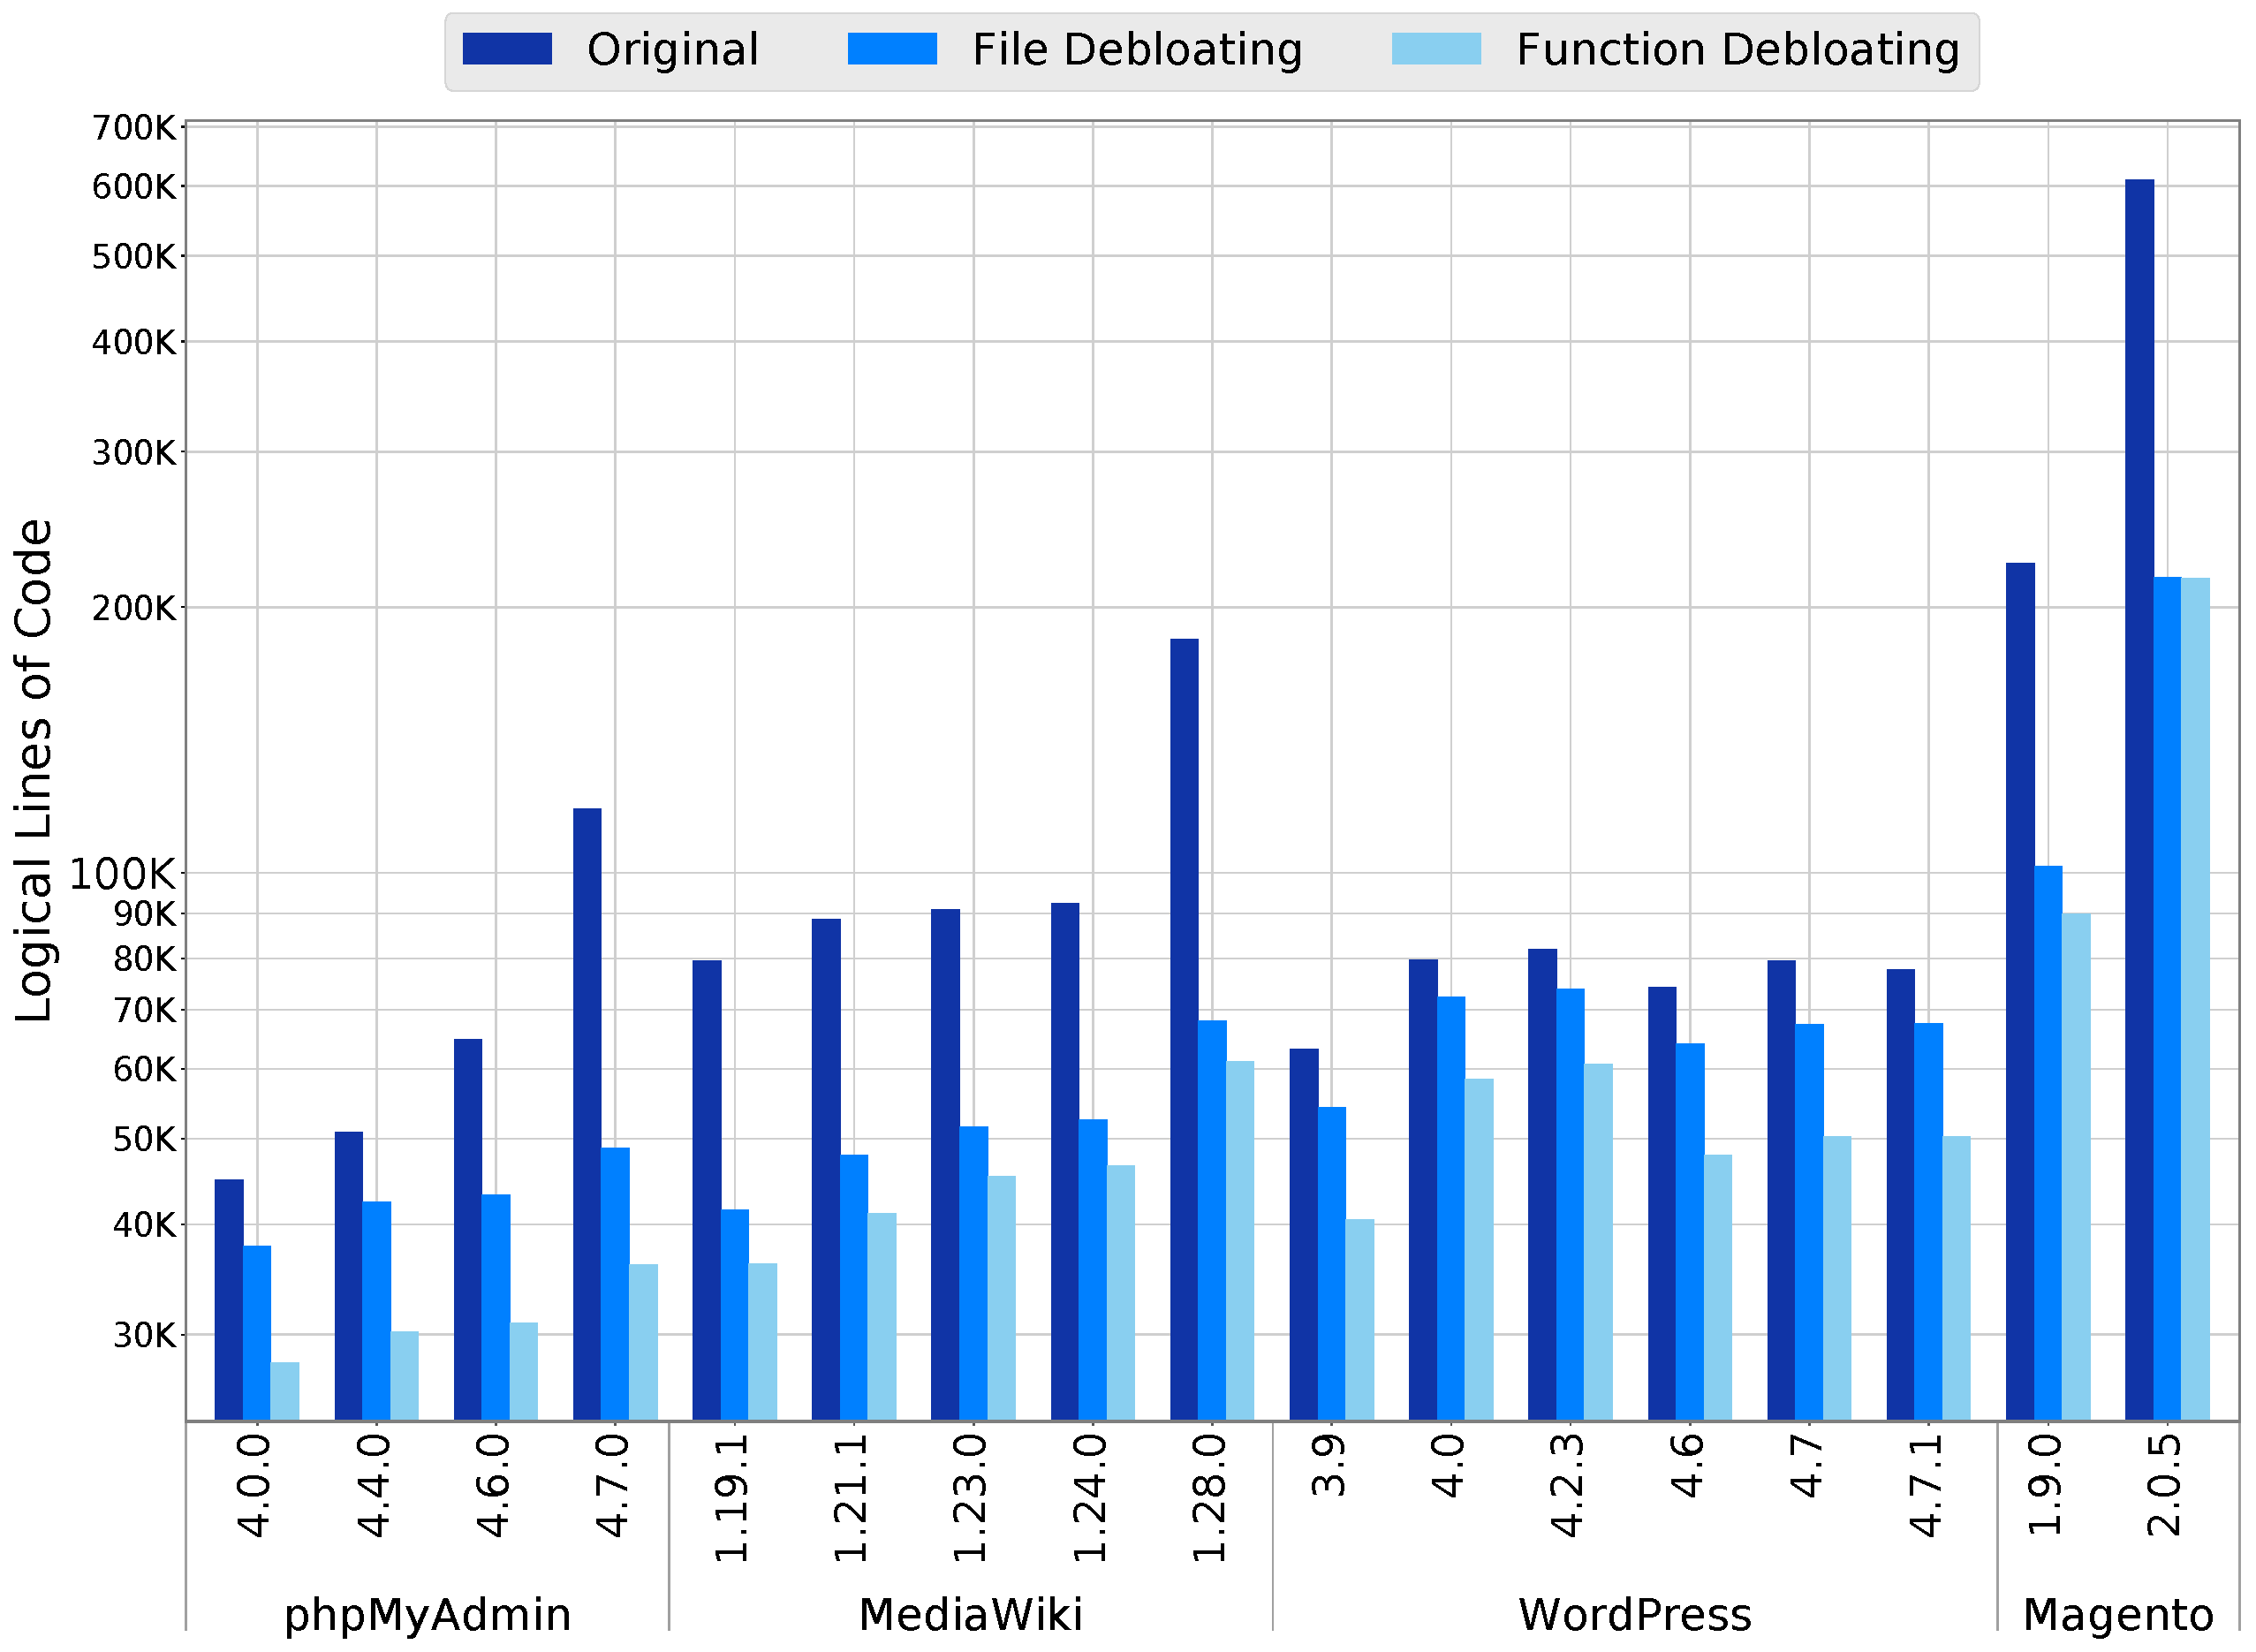
\includegraphics[width=\linewidth]{figures/lim/lloc.pdf}
  \caption{Logical Lines of Code before and after debloating}
  \label{fig:lloc}
\end{figure}


\paragraph{File-level debloating.}
Overall, file-level debloating, the most conservative of the two evaluated
debloating strategies, is already effective in reducing the number of LLOC with an average of 33.1\% reduction.
The minimum observed in our experiment is 9.2\% for WordPress
v.4.0 and a maximum of 64.5\% for Magento v.2.0.5. For Magento,
this reduction represents a removal of 393K lines of code.
This number is a clear sign that large web applications encompass many
different features that may not be used by all users and therefore result
in bloated applications with an unnecessarily large attack surface. At the same time, it is worthwhile repeating that all debloating results presented in this section are conditional to how web applications are used. Therefore, these large levels of debloating cannot be guaranteed for all possible deployments of web applications. We discuss this issue in Section~\ref{sec:limitations}.

\paragraph{Function-level debloating.}
On average, function-level debloating is able to remove 46.8\% of lines of code.
For both Magento and MediaWiki, it can remove up to
7\% more code over file-level debloating. For phpMyAdmin and WordPress, we observe an
increase of debloating capability of up to 24\%. This
larger reduction (compared to MediaWiki and Magento) is mainly due to
the differences in software development practices.

Compared to the other
tested applications, phpMyAdmin and WordPress are more monolithic with a smaller number of large
source-code files. Since file-level debloating only removes files when none
of their functions were executed, the monolithic nature of these two applications resists
this kind of coarse-level debloating. Contrastingly, Magento and MediaWiki
are developed in a much more modular fashion (many small files each responsible
for a small number of well-defined tasks) and therefore lend themselves better to file-level
debloating. The more fine-grained, function-level debloating bypasses this
issue and can therefore reduce the attack surface of a web application,
even for more monolithic web applications.


\subsubsection{Cyclomatic complexity}
\label{subsubsec:cyclomatic-complexity}
Next, we look at the evolution of cyclomatic complexity (CC). CC is defined as
the number of linearly independent paths through the code of
an application~\cite{mccabe1976complexity}. A high CC for a
single class implies complicated code that is difficult to
debug and maintain~\cite{gill1991cyclomatic} and therefore
more prone to contain vulnerabilities when compared to code with low
CC~\cite{shin2008empirical,kurmus2013attack}.

\begin{figure}[t]
  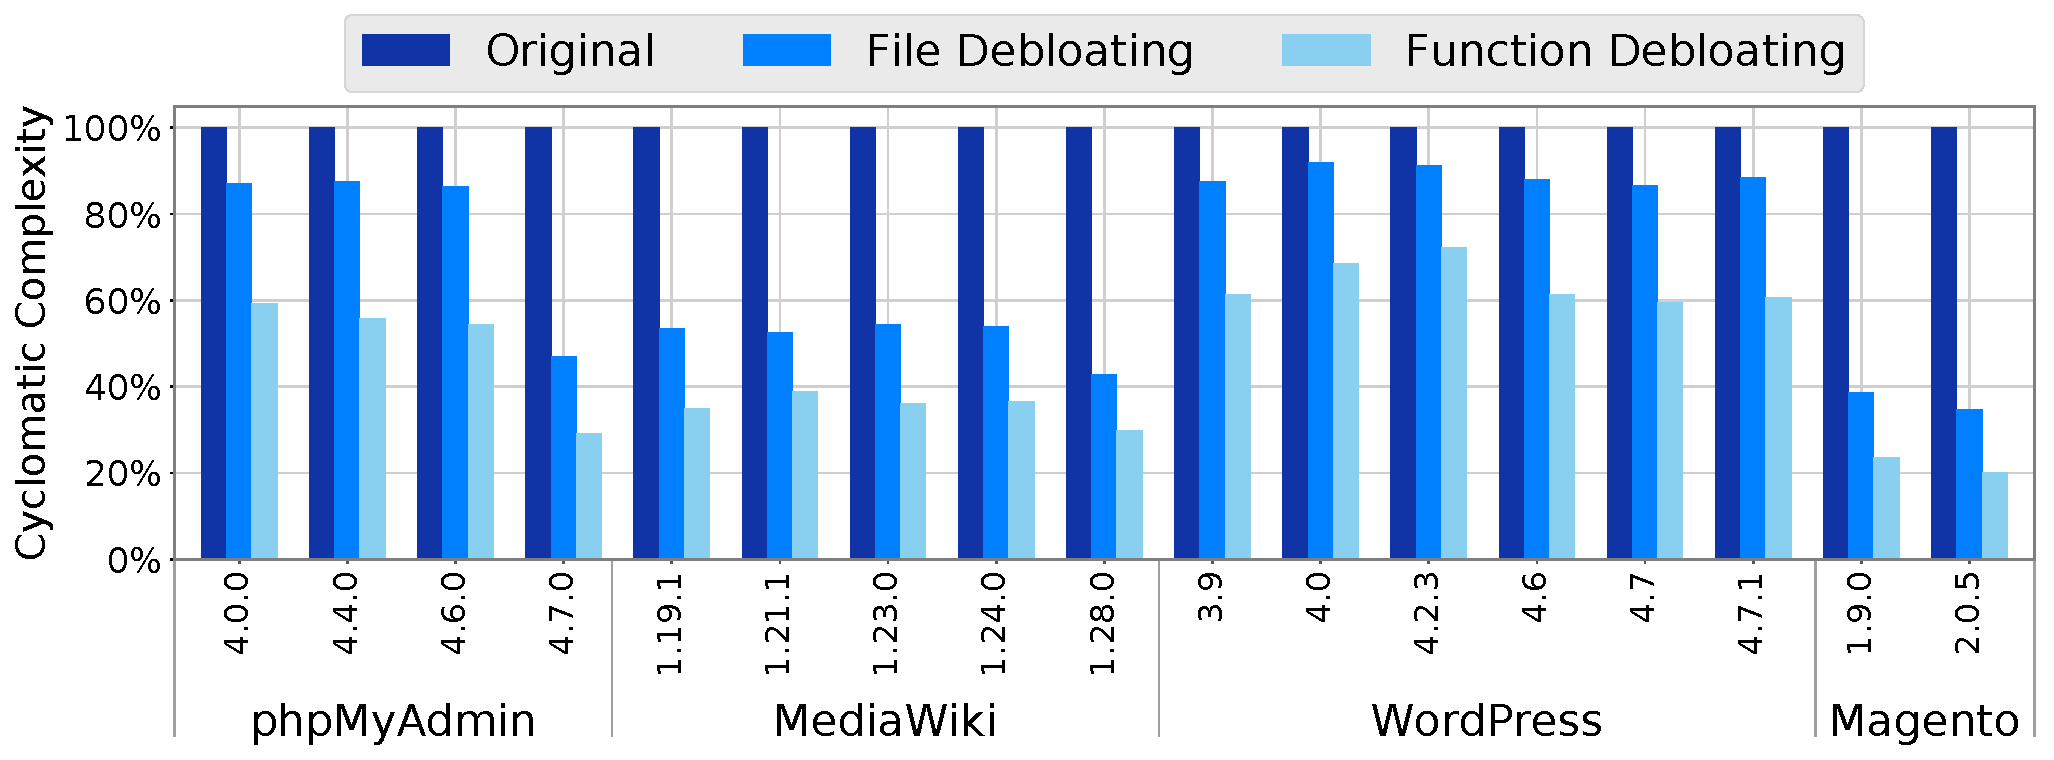
\includegraphics[width=\linewidth]{figures/lim/cc_over_loc.pdf}
  \caption{Evolution of cyclomatic complexity before and after debloating}
  \label{fig:ccoverloc}
\end{figure}

Figure~\ref{fig:ccoverloc} reports on the evolution of the overall CC for
each tested version in our experiment. File-level debloating decreases
CC between 5.9\% to 74.3\% with an average of 32.5\%.
Function-level debloating decreases the program complexity between 23.8\% and 80.2\% with an average of 50.3\%.
These statistics demonstrate that
debloating can remove complex instructions and execution paths in addition to
simple ones. Moreover, the difference between file-level and function-level
debloating shows that code removal through function-level debloating is much
more suited to all kinds of web applications as shown earlier through LLOC
reduction achieved via function-level debloating.


\begin{table}[t]
\caption{Number of CVEs removed after application debloating}
\centering
\scalebox{0.72}{
\begin{tabular}{|c|l|l|l|l|l|}
\hline
\multicolumn{1}{|l|}{\textbf{Application}} & \textbf{Strategy}   & \multicolumn{2}{l|}{\begin{tabular}[c]{@{}l@{}}\textbf{Total}\\ \textbf{Removed CVEs}\end{tabular}} & \multicolumn{2}{l|}{\begin{tabular}[c]{@{}l@{}}\textbf{Removed}\\ \textbf{Exploitable CVEs}\end{tabular}} \\ \hline
\multirow{2}{*}{phpMyAdmin}       & File Debloating     & 4/20                                    & 20 \%                                   & 3/19                                      & 15.7 \%                                     \\ \cline{2-6}
                                  & Function Debloating & 12/20                                   & 60 \%                                   & 11/19                                     & 57.8 \%                                     \\ \hline
\multirow{2}{*}{MediaWiki}        & File Debloating     & 8/21                                    & 38 \%                                   & 3/16                                      & 18.7 \%                                     \\ \cline{2-6}
                                  & Function Debloating & 10/21                                   & 47.6 \%                                 & 5/16                                      & 31.2 \%                                     \\ \hline
\multirow{2}{*}{WordPress}        & File Debloating     & 0/20                                    & 0 \%                                    & 0/20                                      & 0 \%                                        \\ \cline{2-6}
                                  & Function Debloating & 2/20                                    & 10 \%                                   & 2/20                                      & 10 \%                                       \\ \hline
\multirow{2}{*}{Magento}          & File Debloating     & 1/8                                     & 12.5 \%                                 & 1/8                                       & 12.5 \%                                     \\ \cline{2-6}
                                  & Function Debloating & 3/8                                     & 37.5 \%                                 & 3/8                                       & 37.5 \%                                     \\ \hline
\end{tabular}
}
\label{table:debloatingcvesresults}
\end{table}

\subsection{Analysis of CVEs}
In this section, we investigate the number of removed CVEs after debloating
along with the effects of debloating on different vulnerability categories.

\subsubsection{CVE reduction after debloating}
\label{sec:cve_reduction}
One practical way to measure the security benefits of debloating web
applications is to study the effects of debloating on known historical
vulnerabilities. If vulnerabilities were part of the core functionality of the
program, the evaluated debloating strategies will not be able to remove the
code associated with them. However, if some vulnerabilities reside in parts
of a web application that are not commonly used, the process of debloating
can effectively remove them.


Table~\ref{table:debloatingcvesresults} compares the effectiveness of
debloating strategies by listing the fractions of removed CVEs. We consider
a vulnerability to have been successfully removed if all the lines of code
and functions associated with that vulnerability were removed during the
stage of debloating. This is a conservative approach as one modification
performed on a single line could thwart a complete attack. As such, the
numbers we report in this section can be interpreted as lower bounds of
the actual number of removed CVEs.


In terms of configuration, we selected the default one for each application.
However, certain vulnerabilities may not be exploitable under this configuration.
For example, there exists 5 CVEs in our dataset for MediaWiki which require file upload functionality to be enabled. Since this option is disabled by default, we make an explicit distinction in the table.
``Total Removed CVEs'' is the total number of CVEs removed by debloating regardless of whether the vulnerable code is enabled or disabled through a configuration option. ``Removed Exploitable CVEs'' reports on the CVEs that are reachable under default configurations of target web applications.
%Certain vulnerabilities may not be exploited under the default configuration of target applications. For example there exists 5 CVEs in our dataset for MediaWiki which require file upload functionality to be enabled. Since this option is disabled by default,
%we ran our tests with and without this feature enabled and reported both numbers.
%``Total Removed CVEs`` is the the total number of CVEs removed by debloating regardless of vulnerable code being enabled through configuration settings and ``Removed Exploitable CVEs'' reports on the CVEs that are reachable under default configurations of target web applications.

On average, we discovered that up to 38~\% of vulnerabilities are removed by
file debloating whereas 10-60~\% are removed by function debloating. As
shown in Table~\ref{table:debloatingcvesresults}, function-level debloating
can triple (in the case of phpMyAdmin and Magento) the number of removed CVEs, compared to file-level debloating. This
behavior can be generalized to web applications that do not have CVE
information and demonstrates that the reduction of a web application's
LLOC (Section~\ref{subsubsec:lloc}) and its cyclomatic complexity
(Section~\ref{subsubsec:cyclomatic-complexity}) translates to a reduction
of concrete vulnerabilities. Wordpress is a clear negative outlier with only
10\% CVE reduction, even through the more flexible function-debloating
strategy. As mentioned earlier, WordPress is a relatively monolithic
application and most of our mapped CVEs are located in core WordPress code (e.g.,
Authentication, CSRF tokens, and post/comment-related actions) which cannot
be removed by our debloating framework.








\begin{figure}[t]
  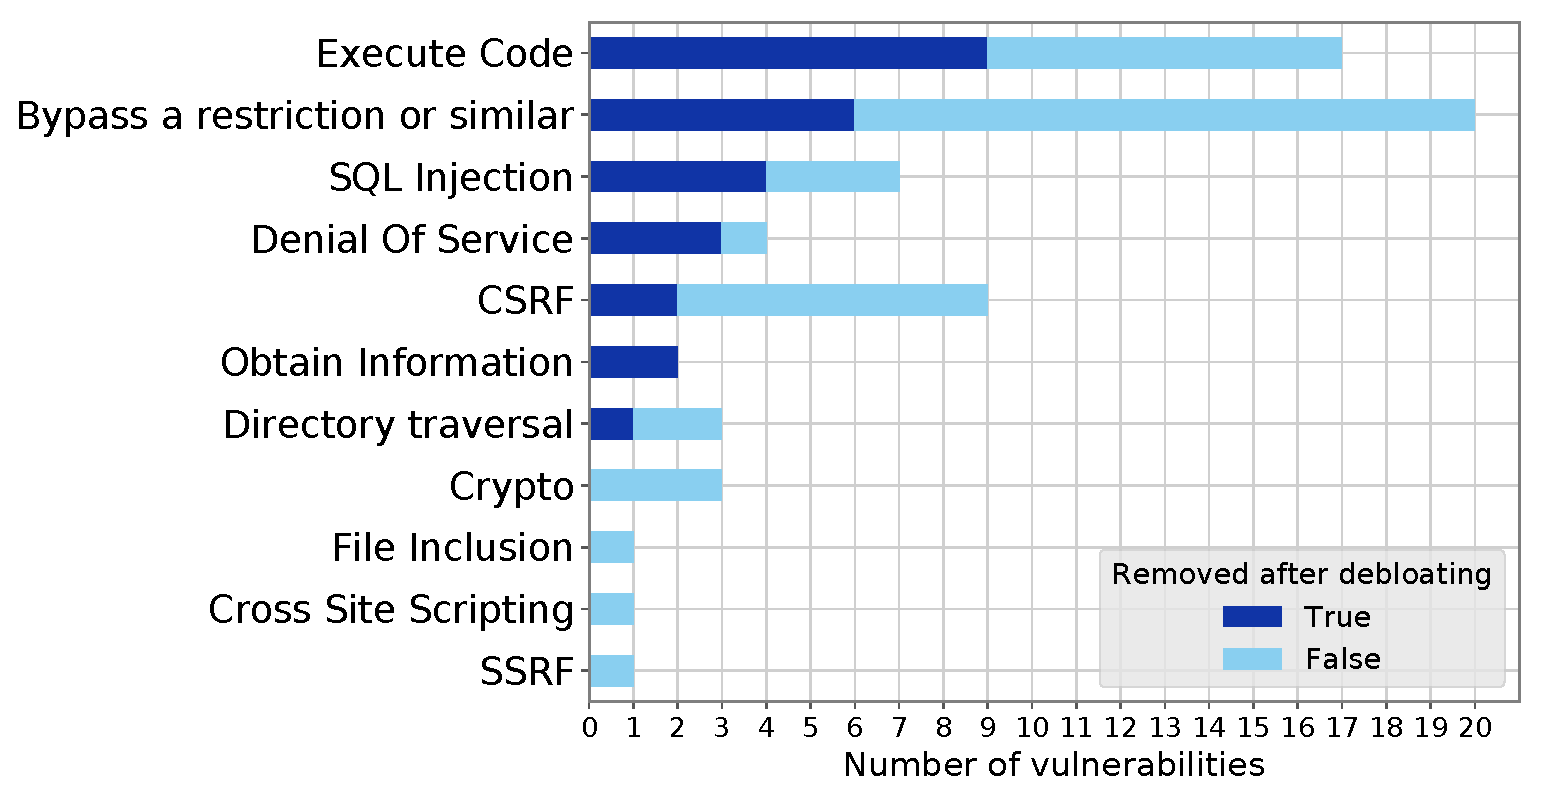
\includegraphics[width=\linewidth]{figures/lim/vuln_per_category.pdf}
  \caption{Vulnerability Categories}
  \label{fig:vulnpercat}
\end{figure}

\subsubsection{Types of CVEs in analyzed web applications}

Even though our results demonstrate the ability to remove vulnerabilities
from web applications through the use of debloating, one may wonder
whether debloating is better suited for some types of vulnerabilities over
others. Figure~\ref{fig:vulnpercat} provides details on the categories of
the CVEs we removed through debloating.


One can observe that for certain classes of vulnerabilities, such as,
Denial-of-Service attacks and Information-Revealing vulnerabilities,
debloating can almost completely remove them.
For others, such as, restriction bypassing, command execution, and
SQL injection, debloating can substantially reduce them.
Our interpretation of these findings has to do with the maturity of
the evaluated web applications. Specifically, all four web applications
have been available for a long period of time, allowing many shallow
vulnerabilities to have already been discovered and corrected. The remaining
vulnerabilities are likely to be situated in parts of a web application that
are less commonly exercised. For example, the code-execution vulnerabilities
that can be removed for phpMyAdmin are inside very specific features, such as,
the ability to export PHP arrays (CVE-2016-6609), the support of the
ZIP extension while importing data (CVE-2016-6633), and the abilities
to copy table definitions (CVE-2013-3238) and perform Regex search and replace over table columns
(CVE-2016-5734).

\begin{table*}[t]
\caption{Statistics on the external packages included in web applications and the effects of debloating in terms of reducing their LLOC.}
\centering
\scalebox{0.5}{
\begin{tabular}{c|c|c|c|c|c|c|c|c|c|}
\cline{2-10}
 & \multicolumn{3}{c|}{\textbf{Before debloating}} & \multicolumn{6}{c|}{\textbf{After function-level debloating}} \\ \hline
\multicolumn{1}{|c|}{\multirow{2}{*}{\textbf{Application}}} & \multirow{2}{*}{\begin{tabular}[c]{@{}c@{}}\# \textit{lines in main}\\\textit{application}\end{tabular}} & \multirow{2}{*}{\begin{tabular}[c]{@{}c@{}}\textit{\# lines in}\\\textit{packages}\end{tabular}} & \multirow{2}{*}{\textit{\# packages}} & \multirow{2}{*}{\begin{tabular}[c]{@{}c@{}}\textit{\# lines in main}\\ \textit{application}\end{tabular}} & \multirow{2}{*}{\begin{tabular}[c]{@{}c@{}}\textit{\# lines in}\\\textit{packages}\end{tabular}} & \multirow{2}{*}{\begin{tabular}[c]{@{}c@{}}\textit{\# packages}\\\textit{completely}\\\textit{removed}\end{tabular}} & \multicolumn{3}{c|}{\begin{tabular}[c]{@{}c@{}}\textit{\# packages where a given \%}\\\textit{lines were removed}\end{tabular}} \\ \cline{8-10}
\multicolumn{1}{|c|}{} &  &  &  &  &  &  & \textgreater{}\textit{70\%} & \begin{tabular}[c]{@{}c@{}}\textless{}\textit{70\% and}\\ \textgreater{}\textit{30\%}\end{tabular} & \textless{}\textit{30\%}\\ \hline
\multicolumn{1}{|c|}{phpMyAdmin 4.7.0} & 35,739  & 82,604  & 45 & 26,377 (-26.2\%)  & 9,653 (-88.3\%)  & 38 (84.4\%) & 2 & 1  & 4  \\ \hline
\multicolumn{1}{|c|}{MediaWiki 1.28.0} & 133,019 & 50,898  & 40 & 54,827 (-58.8\%)  & 6,285 (-87.7\%)  & 24 (60.0\%) & 2 & 2  & 12 \\ \hline
\multicolumn{1}{|c|}{Magento 2.0.5}    & 396,448 & 212,906 & 71 & 181,696 (-54.2\%) & 34,038 (-84.0\%) & 58 (81.7\%) & 6 & 5  & 2  \\ \hline
\end{tabular}
}
\label{table:numberofpackages}
\end{table*}


Contrastingly, the three cryptography-related vulnerabilities we analyzed are
still present in the debloated versions of web applications. One of the CVEs
related to this category is about a flaw in the cookie encryption algorithm in
phpMyAdmin (CVE-2016-6606). Since every page interacts with user
cookies to, at the very least, verify them, vulnerable code cannot be
removed. Another vulnerability in this category relates to an insecure random
number generator used in cryptographic operations by Magento (CVE-2016-6485).
This vulnerability exists in a constructor of the main encryption
classes which is widely used throughout the application. When considered
together, these findings suggest that cryptography-related vulnerabilities
are a core part of web applications and thus unlikely to be removed through
the process of debloating.




\subsection{External packages}
\label{subsec:external}

\subsubsection{Quantifying the bloat from external packages}

In our testbed, phpMyAdmin v.4.7.0, MediaWiki v.1.28.0 and Magento v.2.0.5 rely
on external dependencies that can be downloaded via Composer (WordPress does not rely on external packages). As described in
Section~\ref{sec:background}, Composer is a package manager for PHP (similar
to the NPM manager for NodeJS applications) which allows web applications
to specify which external packages they rely on and have these packages be
tracked and updated.

As we briefly discussed in Section~\ref{subsubsec:lloc}, the number of LLOC of
these three specific versions dramatically
increases (compared to prior versions) because of this dependency on external
packages. Table~\ref{table:numberofpackages} provides statistics on the
number of packages pulled by these applications and how much bloat they
provide against our usage profiles.


First, one can observe that external packages introduce a large amount of
unused code. For all three debloated applications, more than 84\% of their code
was removed from them. This means that the attack surface is unnecessarily
large through the dependency on external packages. The number of removed
lines from external packages for Magento is particularly noteworthy with
more than 178,000 lines of code removed. Moreover, the number of packages
that can be completely removed is also quite large: 84\% for phpMyAdmin,
60\% for MediaWiki and 81\% for Magento. This confirms that most packages
are unnecessary for the usage profiles that we recorded. Finally, focusing
exclusively on the lines of code, phpMyAdmin is the only application where
external packages have more lines than the main application. However, after
debloating, this relationship is reversed with the codebase of phpMyAdmin
being three times the size of the introduced external packages.


Despite the advantages of using package managers (e.g., the ability to track
dependencies and update vulnerable libraries without the need to update
the main application), our findings show that these advantages come at a
considerable cost in terms of unnecessarily expanding the attack surface of
a web application with code that is seldomly executed. As such, developers
must take special care to include the bare minimum of external packages,
knowing the unwanted side-effects that each external package brings.

\subsubsection{Removing POI gadgets}

\paragraph{What are POI gadgets?}
Property Oriented Programing (POP) is an exploitation technique
in PHP which works similarly to Return Oriented Programming
(ROP)~\cite{shacham2007geometry} and is used to exploit PHP Object Injection
(POI) vulnerabilities~\cite{POI}. In this technique, the attacker creates
exploit gadgets from available code in the applications. By chaining
multiple gadgets within the application, an attacker can usually run
arbitrary code, write to arbitrary files, or interact with a database. Dahse
et al. have studied the automatic generation of such gadget chains for PHP
applications~\cite{Dahse:2014:CRA:2660267.2660363}.

\paragraph{PHP unsafe deserialization.}
The PHP language gives developers the ability to serialize arbitrary objects in
order to store them as text, or transfer them over the network. Deserialization
reverses this process, generating PHP objects from serialized data. This
mechanism can be abused by an attacker to load specific classes in the
application and build a gadget chain. Practical examples of this vulnerability
are when \texttt{unserialize} is called on a database field or value of a
field within a cookie that can be manipulated by the users.

Historically, this attack was very difficult to successfully execute. Attackers
could only build gadgets with the classes that were present in the context of
the vulnerable file. They needed insights into how the application was built
in order to know which classes could be abused for gadgets. However, starting
from PHP 5, the \texttt{\_\_autoload()} magic function~\cite{PHPAutoload}
was introduced and unintentionally made exploitation of deserialization
vulnerabilities easier. This new loading feature was beneficial for PHP
developers who did not have to manually include all the files they wanted to
use at the very top of each of their PHP files. It also helped the adoption
of package managers like Composer, as any external dependency could be easily
called from anywhere in the application. The downside of this new function
was that it also allowed attackers to instantiate any PHP class across the
entire application thereby enabling the easier construction of gadget chains.

In order to build a chain, attackers use these so-called ``magic''
functions~\cite{PHPWakeup} that form the basis of their gadget chain. One of
the functions that is widely used in POI exploits is the \textit{destruct}
function. In Section~\ref{subsec:coverage}, we detailed the challenges in
getting complete coverage of destructors in our tested applications. Accurate
coverage of destructors also allows us to precisely analyze the impact of
debloating on gadget creation.




\paragraph{Can debloating remove gadgets from external packages?}

Given the increased footprint of web applications due to their reliance
on package managers and external dependencies, one may wonder about the
possibility of abuse of these packages for the creation of gadgets. To
measure the effect of debloating on Property-Oriented-Programming (POP)
gadgets, we utilized the PHPGGC~\cite{PHPGGC} library. PHPGGC (which stands
for PHP Generic Gadget Chains) contains a list of known gadgets in popular
PHP packages such as Doctrine, Symfony, Laravel, Yii and ZendFramework. When
a vulnerable PHP application includes any of the packages listed in PHPGGC,
the attackers can generate gadget chains to achieve RCE, arbitrary file
writes, and SQL injections.

We analyzed the available gadget chains in PHPGGC and
checked whether any of our tested PHP applications included these
chains. Table~\ref{table:knowngadgets} summarizes the presence of each gadget
and whether debloating removes them or not. WordPress is not included in this table because it does not rely on external packages.
This does not make WordPress immune to POI attacks, but universally known gadget chains in popular external packages can not be used to exploit WordPress.
%Note that while packages such as Symfony are used across our tested web applications, the specific component required to create gadget chains was not pulled by any of tested applications. Such cases are omitted from our results.
For the affected applications, file-level debloating removes 4/6 gadgets while function debloating removes
6/6 available gadget chains. This again demonstrates the power of debloating
which can not only remove some fraction of vulnerabilities but also make
the exploitation of the remaining ones harder by removing the gadgets that
attackers could abuse during a POI attack.


\begin{table}[]
  \centering
  \caption{List of packages with known POP gadget chains}
\scalebox{0.9}{
\begin{tabular}{|l|l|c|c|}
\hline
\multirow{2}{*}{\textbf{Application}}      & \multirow{2}{*}{\textbf{Package}} & \multicolumn{2}{l|}{\begin{tabular}[c]{c@{}c@{}}\textbf{Removed by}\\\textbf{Debloating}\end{tabular}} \\ \cline{3-4}
    &    & \textit{File}     &  \textit{Function}                                     \\ \hline
\multirow{2}{*}{phpMyAdmin 4.7.0} & Doctrine                 & \faCheck                                         & \faCheck                                            \\ \cline{2-4}
                                  & Guzzle                   & \faCheck                                         & \faCheck                                            \\ \hline
MediaWiki 1.28.0                  & Monolog                  & \faCheck                                         & \faCheck                                            \\ \hline
\multirow{3}{*}{Magento 2.0.5}    & Doctrine                 & \faCheck                                         & \faCheck                                            \\ \cline{2-4}
                                  & Monolog                  & \faTimes                                         & \faCheck                                            \\ \cline{2-4}
                                  & Zendframework            & \faTimes                                         & \faCheck                                            \\ \hline
\end{tabular}}
\label{table:knowngadgets}
\end{table}


\subsubsection{Utilizing development packages in production}
During our analysis of external packages, we identified yet another source
of bloat in new versions of web applications. When declaring external
dependencies through Composer, two options are available: ``require'' and
``require-dev''. The first option indicates packages that are mandatory for
the application to run properly. The second lists packages that should only be
used in development environments, such as, packages providing support for unit
testing, performance analysis, and profiling. We discovered that applications
downloaded from official websites often include these development packages. As
such, when these packages are used to deploy web applications in production
mode, they will contain unnecessary development libraries. This does not
only increase the attack surface by having unnecessary code bloating the
application, but can also lead to exploitation for misconfigured applications.

CVE-2017-9841 presents one example of such a
vulnerability~\cite{phpunitVulnerability}. Specifically, this CVE refers
to an RCE attack in specific versions of the PHPUnit library, which is
a popular unit testing library for PHP. By default, Composer places all
external packages under ``vendor'' directory. If this specific directory
happens to be accessible through a misconfiguration of the server, PHPUnit
files are then accessible and can be exploited to conduct an RCE attack.

The four web applications that we evaluated for this study, present
different behaviors with respect to development packages. WordPress does not rely on external packages downloaded through Composer.
MediaWiki never
included development packages in its releases. phpMyAdmin had them in version
4.7.0 but stopped including them in version 4.8.3 (the latest at the time of
writing). Magento started including them from version 2.0 and still includes
them today. We have reached out to Magento and informed them about this issue.


\subsection{Qualitative analysis of the removed code}
\label{subsec:qualitative}

In the previous sections, we analyzed the effects of debloating on the source code of applications from a software-engineering perspective (i.e., LLOC and Cyclomatic Complexity reduction) as well as from a security standpoint (i.e., number of CVEs and gadgets removed). At the same time, one may wonder what exactly was removed from each application during the process of debloating.



Given that thousands of files were removed, manually analyzing each file does not scale. As such, we turn to NLP techniques that allow us to cluster the removed files together and provide us with hints about the nature of each cluster. Specifically, we use the k-means clustering algorithm based on text vectors extracted from removed file names and file paths. Each file path includes directories that indicate which library or package, the file belongs to. For most modern web applications, this allows for a reasonable separation of files across different application plugins and modules.
To end up with meaningful clusters, we tuned TFIDF vectorizer parameters along with the number of k-means clusters. We used the TFIDF maximum frequency limit to ignore common terms appearing in more than 50\% of the files. Depending on the size and modularity of the application, 10 to 20 clusters yielded the most instructive grouping of files.

Table~\ref{tab:removed_files_categories} shows the categories of the three largest removed clusters from each web application. Across all four applications, we observe the removal of source code related to external packages (e.g., Symfony for phpMyAdmin, Elastica for MediaWiki, and Zendframework1 for Magento), followed by localization/theme files (e.g., twentyfourteen theme for WordPress), and unused database drivers. We provide more application-specific details of removed features in the next paragraphs.

\begin{table}[t]
  \caption{Features and external packages with the most removed files after file debloating (removed features are marked in italic). Entries marked with $\ast$ are packages that are indirectly pulled by other ``require-dev'' packages (not used by core application) for the purpose of test coverage reporting and coding standard enforcement.}
  \label{tab:removed_files_categories}
  \centering
\scalebox{0.75}{
\begin{tabular}{|l|l|}
\hline
\textbf{Applications} & \textbf{Features/Packages with most files removed} \\ \hline
                           & 1) Guzzle~\cite{guzzle}: ``Generating API HTTP response'' *  \\
\textit{phpMyAdmin 4.7.0}  & 2) Symfony~\cite{Symfony}: ``Parsing configuration files'' * \\
                           & 3) PHP\_CodeSniffer~\cite{PHP_CodeSniffer}: ``Enforcing coding standards'' * \\ \hline
                           & 1) \textit{Messages \& Languages} \\
\textit{MediaWiki 1.28.0}  & 2) Less.php~\cite{less.php}: ``Generating CSS code'' \\
		                       & 3) Elastica~\cite{elastica}: ``Elastic search interface used by\\ & extensions'' \\ \hline
                           & 1) Twentyfourteen theme~\cite{twentyfourteen_theme} \\
\textit{WordPress 4.7.1}	 & 2) Twentytwelve theme~\cite{twentytwelve_theme} \\
		                       & 3-4) Also theme related \\
		                       & 5) \textit{Multi-site administration} \\ \hline
	                         & 1) Zendframework1~\cite{zendframework1}: ``Generating web pages and\\
\textit{Magento 2.0.5}     & database operations'' \\
		                       & 2) \textit{Sales, Orders \& Credit Memo} \\
		                       & 3) \textit{Internal framework filters \& Views} \\ \hline
\end{tabular}
}
\end{table}

\vspace{0.5ex}
\noindent\textbf{phpMyAdmin's} removed features include the uploading of plugins, GIS visualizations, and unused file formats used in import/export (such as, Dia, EPS, PDF, SVG, and ZIP). In addition, debloating removed unused plugins and external packages which make up the top 3 features removed from this web application as shown in Table~\ref{tab:removed_files_categories}. phpMyAdmin version 4.6.0 and 4.7.0 include unit tests which are also removed by our system. The LLOC for the removed test files is less than 2\% of the whole code base of the application.

\vspace{0.5ex}
\noindent\textbf{MediaWiki} provides an API to interact with the wiki which is separate from the regular web interface that users interact with. Most actions within this API, including queries, file upload, and non-default output formats for this API were removed. Top categories of removed files consist of localization of messages and language files in addition to external dependencies (Lines 2 and 3) as listed in Table~\ref{tab:removed_files_categories}. The debloating process also removes file-upload modules which are disabled, by default, in MediaWiki. It is important to note that even if a module is ``disabled,'' the code still resides on the server and could be abused by specific types of attacks. For example, in a recent attack against a WordPress plugin, the vulnerability could be exploited even if that plugin was disabled~\cite{wordpressPlugin}. Debloating \textit{removes} the source code of disabled and unused features and therefore does not suffer from this type of attack.
Finally, the process of debloating, removed unused extensions of Mediawiki (e.g., citation, input box, pdf handler, poem and syntax highlighting). Mediawiki 1.19.1 and 1.28.0 include unit tests, and they measure less than 1.5\% of LLOC in the whole code base of their respective versions.

\vspace{0.5ex}
\noindent\textbf{WordPress} takes a slightly different approach where the core functionality is concentrated in a relatively small number of large PHP files. The removed features of WordPress include installation files, unused modules (FTP, multi-site, user registration), disabled themes and update files (note that we could not exercise update files during our tests because this would change the version of the evaluated web application and create inconsistencies in our analysis of removed CVEs). In terms of testing, the installation files that we obtained from the WordPress website do not contain any unit tests.

%Interestingly, WordPress contains less code bloat. That is because most of the functionality within this application is exercised by tutorials and other tests, and this is not the result of more comprehensive tutorials. As WordPress has a monolithic nature that does not rely on external dependencies (the main source of bloat), the application does not include unnecessary features that only a subset of users would use. WordPress offloads these specific requirements to plugins. For instance, importing data into WordPress which is available in other studied software requires a separate plugin. As a result, most of the existing modules in vanilla WordPress would be exercised throughout the dynamic analysis tests with the exception of few that are mentioned above. This also affects the mapped CVEs for core WordPress in that the CVEs mostly target core functionality (e.g., Authentication, CSRF tokens and post and comment related actions).

\vspace{0.5ex}
\noindent\textbf{Magento} consists of both external packages and internal modules. We observed that various internal modules were removed, including an XML API for mobile, wishlists, ratings, and specific payment modules (such as, Paypal). Since many packages and internal modules include the terms ``sales,'' ``orders,'' and ``tax,'' these individual files across multiple modules were clustered into the same category by k-means. Finally, Magento 1.9.0 does not include unit tests while the test files included in Magento 2.0.5 and its external packages measure up to 15\% of its code base. For Magento 2.0.5, Zendframework1 which is an external dependency has most of its files removed by debloating.

%\begin{table}[]
%  \caption{Top file categories removed by file debloating}
%  \label{tab:removed_files_categories}
%  \centering
%\scalebox{0.8}{
%\begin{tabular}{|l|}
%\hline
%\multicolumn{1}{|c|}{\textbf{Applications}}                        \\ \hline
%\multicolumn{1}{|l|}{\textbf{phpMyAdmin 4.7.0:}}                                                           \\ %\hline
%1) Guzzle 2) Symphony 3) squizlabs/php\_codesniffer                                              \\ \hline
%\multicolumn{1}{|l|}{\textbf{MediaWiki 1.28.0:}}                                                           \\ %\hline
%1) Messages \& Languages 2) oyejorge/less.php 3) ruflin/elastica                                 \\ \hline
%\multicolumn{1}{|l|}{\textbf{WordPress 4.7.1:}}                                                            \\ %\hline
%1) twentyfourteen theme 2) twentytwelve theme (3/4 are also themes) \\ 5) multi-site administration \\ \hline
%\multicolumn{1}{|l|}{\textbf{Magento 2.0.5:}}                                                              \\ %\hline
%1) Zendframework1 2) Sales, Orders \& Creditmemo \\ 3) Internal framework filters \& views          \\ \hline
%\end{tabular}
%}
%\end{table}



% Summary of removed features
%--- 4.0.0 ---
%
%Tracking, triggers, gis data, unused engines (berkeleydb, binlog, memory, myisam, ndbcluster)
%Unused encryption functions.
%Unused authentication mechanisms
%Uploading plugins
%Unused plugin transformations (Image inline or link, text to formats such as date)
%Export schema formats such as: Dia, Eps, Pdf, SVG and Visio.
%Zip extension.
%setup files.
%
%--- 4.6 ---
%
%Recaptcha plugin, Unused sql parser modules, test files.
%
%--- 4.7 ---
%
%External packages: doctrine/instantiator, gitonomy/gitlib, google/recaptcha, guzzle/guzzle, phpdocumentor, phpmyadmin/sql-parser, phpspec/prophecy, phpunit/php-code-coverage, timer, php-token-stream, %satooshi/php-coveralls, sebastian/comparator, sebastian/diff, sebastian/global-state, squizlabs/php\_codesniffer, symfony/cache, symfony/config, symfony/console, symfony/debug, symfony/event-dispatcher, %symfony/expression-language, symfony/filesystem, symfony/polyfill-mbstring, symfony/process, tecnickcom/tcpdf and webmozart.
%
%Mediawiki:
%
%--- 1.19.1 ---
%
%Unused APIs including: Formats such as JSON, PHP, XML, YAML, txt and raw. Action APIs: Authentication, Queries, Fileupload.
%Caching such as memcached, object file and resource file cache.
%Database drivers such as: MSSQL, Postgres, Oracle, Sqlite and db2.
%File repo
%Installation files.
%Media formats such as DjVu, GIF, PNG, SVG and XMP.
%Parser tools such as diff and hasher.
%Profiler and Tracer tools.
%Search modules for unused database drivers.
%Upload modules such as upload from URL, stash or upload in chunks.
%Unused language files and skins.
%Maintenance files such as benchmarks and clean up files.
%
%--- 1.21.1 ---
%
%Extensions such as citation, confirm edit, gadgets, image map, input box, interwiki, pdf handler, poem, rename user, syntax highlighting and title blacklists.
%
%--- 1.28.0 ---
%
%debug loggers, ``Exceptions!'', export to formats such as 7zip, bzip, dbzip2 and gzip.
%redis db modules, xml module, mail, rcfeed (machine readable recent changes)
%External packages: semver, cssjanus, php-jwt, james-heinrich/getid3, justinrainbow/json-schema, liuggio/statsd-php-client, monolog, kafka-php, oojs-ui, less.php, pear, pimple, ruflin/elastica, symfony/%process, vendor/wikimedia and zordius/lightncandy.
%
%Magento
%
%...
%
%WordPress:
%
%--- 3.9 ---
%
%FTP files, installation files, multisite modules, unused themes, sign up and new account activation, mail and trackback, cron and update file.
%
%--- 4.0 ---
%
%Export links from one blog to another. (opml)
%
%--- 4.7 ---
%
%pclzip library, fix corrupted database.

%\begin{table*}[]
%  \caption{Top file categories removed by file debloating}
%  \label{tab:removed_files_categories}
%  \centering
%\scalebox{0.69}{
%\begin{tabular}{|l|l|}
%\hline
%\textbf{Application}      & \textbf{Top file categories removed by debloating}                                                                                              \\ \hline
%phpMyAdmin 4.7.0 & 1) Guzzle 2) Symphony 3) squizlabs/php\_codesniffer 4) PHPUnit 5) phpsec/prophecy                                                                        \\ \hline
%MediaWiki 1.28.0 & 1) Messages \& Languages 2) oyejorge/less.php 3) ruflin/elastica 4) Installer \& Maintenance 5)james-heinrich/getid3                                     \\ \hline
%WordPress 4.7.1  & 1) twentyfourteen theme 2) twentytwelve theme 3) twentythirteen theme 4) twentytwelve theme 5) multi-site administration                                 \\ \hline
%Magento 2.0.5    & 1) Zendframework1 2) Sales, Orders \& Creditmemo 3) Internal framework filters \& views 4) Products, Sales, Shipping \& Tax 5) Widgets, Wishlists \& CMS \\ \hline
%\end{tabular}
%}
%\end{table*}
%}

\subsection{Testing debloated web applications against real exploits}
\label{section:metasploit}
To ensure the correct mapping of CVEs to source code and the ability of debloating to stop real attacks, we collected 4 exploits available in the Metasploit framework and augmented them with 4 POCs that we developed based on public bug-tracker records and vulnerability details. After verifying that we can successfully exploit the original versions of the evaluated web applications, we tested the same exploits on the debloated versions. Half of the previously successful exploits failed because the vulnerable code was removed during the process of debloating. Table~\ref{table:metasploit_vulns} lists the tested exploits against original and debloated applications.

As before, this demonstrates that while debloating is not a panacea against all possible issues, it can substantially improve the security of web applications. Finally, we present a demonstration of CVE-2016-4010 on Magento 2.0.5 in the following video: \url{https://vimeo.com/328225679}.



\begin{table}[]
  \centering
  \caption{Verifying exploitability of vulnerabilities by testing exploits against original \& debloated web applications}
  \label{table:metasploit_vulns}
  \scalebox{0.81}{
\begin{tabular}{|l|l|c|c|}
\hline
\multirow{2}{*}{\textbf{CVE}} & \multirow{2}{*}{\textbf{Target Software}} & \multicolumn{2}{c|}{\textbf{Exploit Successful?}} \\ \cline{3-4}
                     &                                  & \textbf{Original}           & \textbf{Debloated}          \\ \hline
CVE-2013-3238   & phpMyAdmin 4.0.0       & \faCheck & \faCheck                                                             \\ \hline
CVE-2016-5734   & phpMyAdmin 4.4.0       & \faCheck & \faTimes                                                             \\ \hline
CVE-2014-1610   & MediaWiki 1.21.1       & \faCheck & \faCheck                                                             \\ \hline
CVE-2017-0362   & MediaWiki 1.28.0       & \faCheck & \faTimes                                                             \\ \hline
CVE-2018-20714  & WordPress 3.9          & \faCheck & \faCheck                                                             \\ \hline
CVE-2015-5731   & WordPress 4.2.3        & \faCheck & \faCheck                                                             \\ \hline
CVE-2016-4010   & Magento 2.0.5          & \faCheck & \faTimes                                                             \\ \hline
CVE-2018-5301   & Magento 2.0.5          & \faCheck & \faTimes                                                             \\ \hline
\end{tabular}
}
\end{table}

\section{Performance analysis}
\label{subsection:performance}
It is known that code-coverage tools impose a non-negligible overhead on web applications~\cite{xdebug-performance1}. In this section, we report on the results of conducting all the Selenium tests with and without \texttt{XDebug} (our chosen PHP profiler) while measuring execution time, and recording server-side CPU usage and memory consumption. Table~\ref{table:performance} presents the overall results and Figure~\ref{fig:cpu} focuses on CPU consumption.

\begin{table}[]
  \centering
  \caption{Measurements of the execution time, the CPU and memory consumption for the tested web applications with XDebug and Code Coverage (CC) and without XDebug. The reported values for the CPU and memory correspond to the average for each application.}
  \label{table:performance}
\scalebox{0.7}{
\begin{tabular}{|c|c|c|c|c|}
\hline
\multicolumn{2}{|c|}{\textbf{Application}}              & \textbf{Execution (s)} & \textbf{CPU (\%)}       & \textbf{Memory (\%)}   \\ \hline
Magento     & \textit{Without XDebug} & 317           & 21.7           & 10.7          \\ \cline{2-5}
2.0.5       & \textit{With CC}    & 584 (x1.85)   & 56.9 (x2.62)   & 11.82 (x1.10) \\ \hline
MediaWiki   & \textit{Without XDebug} & 36            & 30.7           & 5.2           \\ \cline{2-5}
1.2.8       & \textit{With CC}    & 121 (x3.38)   & 79.3 (x2.58)   & 6.9 (x1.31)   \\ \hline
phpMyAdmin  & \textit{Without XDebug} & 102           & 3.7            & 5.7           \\ \cline{2-5}
4.7.0       & \textit{With CC}    & 116 (x1.14)   & 31.5 (x8.47)   & 5.6 (x0.97)   \\ \hline
WordPress   & \textit{Without XDebug} & 68            & 8.2            & 8.2           \\ \cline{2-5}
4.7.1       & \textit{With CC}    & 170 (x2.50)   & 42.6 (x5.22)   & 12.5 (x1.53)  \\ \hline
\end{tabular}
}
\end{table}

First, looking at the execution time, we can see that code coverage has a
varying impact on the tested web applications.
On one hand, phpMyAdmin is lightly affected with a 14\% increase.
On the other hand, the time it takes to run all tests for MediaWiki has
tripled.
For CPU consumption, the overhead is noticeable and all applications at
least double their use of resources when code coverage is active.
phpMyAdmin is exhibiting the biggest performance hit with a reported
average almost 9 times higher than the one from the base application.
Figure~\ref{fig:cpu} shows that all median values are higher for applications
with \texttt{XDebug} and most applications, at some point, require a second
core with values above 100\%. Finally, in terms of memory consumption,
the server-side code profiler incurs a relatively modest increase for most
applications. The worst overhead is observed when evaluating WordPress with
an increase of 4.3\% of the total device memory (16GB), i.e., an additional
700MB of RAM.

\begin{figure}[t]
  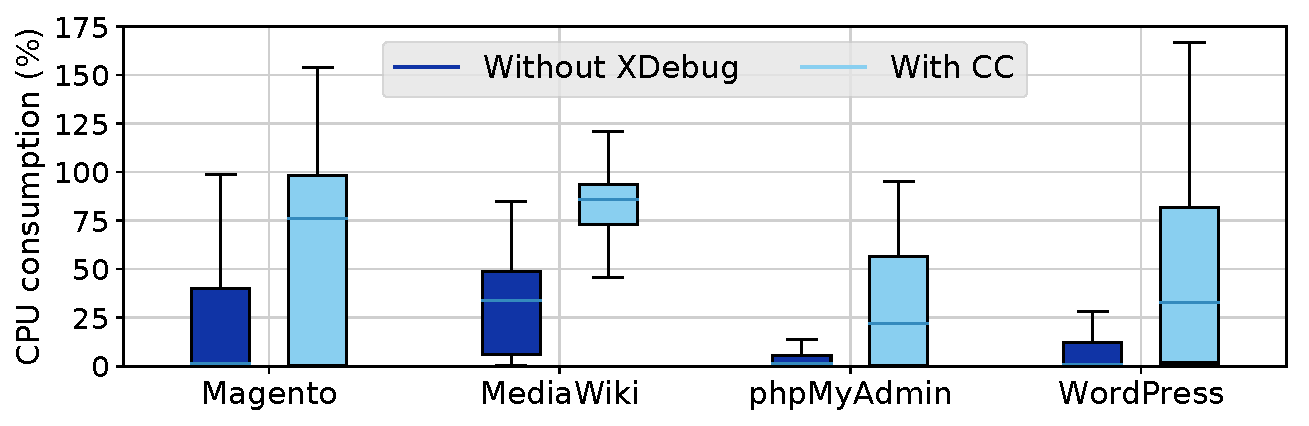
\includegraphics[width=\linewidth]{figures/lim/cpu.pdf}
  \caption{Measurement of the CPU consumption for the tested web
  applications. 100\% corresponds to the use of a single CPU core.}
  \label{fig:cpu}
\end{figure}

Even though our results show that the overall overhead is substantial, it is
important to note that this overhead is not the overhead of the debloated
web applications. Debloated web applications do not require code-coverage
statistics and will therefore execute in the exact same environment as
the original application (i.e., without \texttt{XDebug}). Depending on how
code-coverage information is obtained, this overhead may or may not be an
issue. For example, if the coverage is calculated in an offline fashion
where traces of application usage are replayed against a testing system,
this overhead will have no impact on the real production systems. To allow
for the online computation of code coverage (using real-time user traffic),
we need more optimized code profilers. For example, \texttt{XDebug} currently
overloads 43 opcodes to obtain line-level code-coverage information that
is more fine-grained than required by our debloating techniques and incurs
an unnecessary performance overhead~\cite{xdebug-performance2}. We leave
the development and evaluation of faster code profilers for future work.

\section{Limitations and future work}
\label{sec:limitations}
In this study, we set out to precisely quantify the security benefits of
debloating, when applied to web applications. Through a series of experiments,
we demonstrated that debloating web applications has a number of very
concrete advantages. We showed that debloating can, on average, decrease an
application's code base by removing hundreds of thousands of lines of code,
reduce its cyclomatic complexity by 30-50\% and remove code associated with
up to half of historical CVEs. Moreover, even for vulnerabilities that could
not be removed, debloating can remove gadgets that makes their exploitation
significantly harder. Next, we discuss some of the inherent and technical limitations of our approach and future direction.

\vspace{1ex}

\noindent\textbf{Lack of available exploits:} The number of exploits publicly available compared to the total number of registered CVEs is low. At the same time, the effort to study vulnerability reports, find the relevant patch or bug report, and track the actual vulnerability down to source code level takes a non-negligible amount of manual labor.
% Moreover, these public exploits usually favor certain types of vulnerabilities over others (e.g., favoring remote-command execution over XSS).
This lack of available exploits limits our ability to test the exploitability of vulnerabilities before debloating since certain vulnerabilities might only be exploitable under specific configurations.
For example the set of five file-upload-related vulnerabilities in our MediaWiki dataset (marked as gray in Table~\ref{table:listofallcves}) require access to file upload functionality which is disabled by default. A maintained set of automated, replayable exploits against popular web applications similar to ``BugBox'' introduced by Nilson et al. in 2013, could substantially help researchers at this step\cite{bugbox}.

To address this issue, we mapped the CVEs to features within those applications. This is done by studying the architecture of
target applications based on documentation within the code and available on their websites. We marked a CVE as unexploitable if the underlying feature is disabled by default, and online tutorials in our dataset do not
require users to enable that functionality. This limitation only applies to reported numbers on removed CVEs and does not affect our results on POI gadgets since their mere existence is enough for them to be used in gadget chains.

Our approach results in lower bounds for CVE removal since disabling modules through application configuration does not guarantee removal of all code paths that trigger those modules. Taking CVE-2019-6703 as an example, a vulnerability was discovered in the WordPress ``Total Donations'' plugin~\cite{wordpressPlugin} and disabling this plugin did not prevent attackers from invoking the vulnerable end point and running their exploits.

\vspace{1ex}
\noindent\textbf{Dynamic code coverage:}  Given our reliance on dynamic
code-coverage techniques, it is clear that the success of debloating a web application
is tightly related to its usage profile. Even though we constructed profiles
in a way that is reproducible and unbiased (i.e., by relying on external
popular tutorials, monkey testing, crawlers, and vulnerability scanners), we cannot claim that
real web users would not trigger code that was removed during the stage of
debloating, while they are interacting with a debloated web application.

More specifically, our modeled usage profiles do not cover all possible benign states of target web applications as we assume that users do not use all available features.
Our intuition behind debloating proves to be successful to a large degree since removing unnecessary features brings clear security improvements.
At the same time, our current usage model may not cover deep error states (e.g., logical errors in multi-stage form submissions, or the invalid structure of uploaded files).
As such, we intend to follow-up this work with crowd sourcing and user studies
to understand how administrators, developers, and regular users utilize the
evaluated web applications and whether their usage profiles would allow for
similar levels of debloating.

Due to nature of our approach, we can not take advantage of standard
static-analysis techniques, since we aim to remove the features that are
not useful for a given set of users, not those that are not reachable by
other code. Using static analysis would greatly overestimate the code that
needs to be maintained through the process of debloating and the resulting
web application would contain code (and therefore vulnerabilities) that is
not useful to all users. Going forward, we envision a hybrid approach where
dynamic analysis is used as a first step to identify the core features that
are useful for a specific set of users. These features can then be used as
a starting point for a follow-up static analysis phase to ensure that all
code related to these features is maintained when debloating a web application.

\vspace{1ex}
\noindent\textbf{Handling requests to removed code:}
A separate issue is that of handling requests to removed code. Our
current prototype utilizes assertions to log these requests so that we can
investigate why the corresponding server-side code was not captured by our
coverage profiler. When real users utilize debloated web applications,
one must decide how these failures (i.e., client-side requests requiring
server-side code that was removed) will be handled. Assuming that cleanly
exiting the application and showing an error to the user is not sufficient,
we need methods to authenticate the user's request, determine whether the
request is a benign one (and not a malicious request that aims to exploit
the debloated web application) and potentially re-introduce the removed
code. The client/server architecture of web applications lends itself well
to this model since the web server can decide to re-introduce debloated code
and handle the user's request, without any knowledge of this happening from
the side of the user. All of this, however, requires server-side systems
to introduce the code at the right time and for the appropriate users. We
leave the design of such systems for future work.

\vspace{1ex}
\noindent\textbf{Metrics to measure debloating effectiveness:}
In this paper, we use Cyclomatic Complexity (CC), Logical Lines of Code
(LLOC), reduction in historical CVEs, and POP gadget reduction as four metrics to measure the
effects of debloating on different web applications. However, not every line of code
contributes equally to a program's attack surface. For example, 15\% of removed
files from Magento 2.0.5 are test files for external packages and
the core of the application. Such code may not be directly exploitable or
used in a POP chain unless there is a misconfiguration (e.g., autoloading
including these files, or the directories being publicly accessible). As such,
the resulted reduction in source code metrics (CC and LLOC) may also reflect the code
that does not contribute to the attack surface.
Contrastingly, the reduction of exploitable CVEs draws a more realistic picture
of real world attacks. The drawback of this metric is its unavailability for
proprietary software and the manual effort required to map CVEs to source
code and verify their exploitability.

\vspace{1ex}
\noindent\textbf{Debloating effectiveness:}
Through our debloating experiments we discovered that, in terms of debloating,
not all applications are ``equal.'' Modular web applications debloat
significantly better than monolithic ones (such as WordPress). We hope that
our findings will inspire different debloating strategies that lend themselves
better to monolithic web applications which resist our current function-level
and file-level debloating strategies.




%Finally, this study focuses on the feasibility of debloating based on usage profiles. We tried to model the behavior of general users of these applications through tutorials and other mechanisms, but production environments are vastly versatile in terms of usage of application features
%and the full potential of debloating is ultimately based on the users of instances of applications. As such, efforts to tune the performance of our system and its dependencies to their full potential
%are left for future.

% \section{Related work}
\label{sec:related}

Over the years, different approaches that target very different parts of the
software stack have been studied in the context of software debloating.

\subsection{Debloating for the web}

Despite the importance of the web platform, there has been very little work that attempts to apply debloating to it. Snyder et al. investigated the costs and
benefits of giving websites access to all available browser features through
JavaScript~\cite{snyder2017vibrate}. The authors evaluated the use of different
JavaScript APIs in the wild and proposed the use of a client-side extension
which controls which APIs any given website would get access to, depending
on that website's level of trust. Schwarz et al. similarly utilize a browser
extension to limit the attack-surface of Chrome and show that they are able
to protect users against micro-architectural and side-channel
attacks~\cite{Schwarz2018}. These studies are orthogonal to our work since
they both focus on the client-side of the web platform, whereas we focus on
the server-side web applications.


%boomsma2012Dead
Boomsma et al. performed dynamic profiling of a custom web application
(a PHP application from an industry partner)~\cite{boomsma2012Dead}. The
authors measured the time it takes for their dynamic profile system to get
complete coverage and the percentage of files that they could remove. Since the
application was a custom one, the authors were not able to report specifics
in terms of the reduction of the programs attack-surface, as that relates
to CVEs. Contrastingly, by focusing on popular web applications, and utilizing function-level as well as file-level debloating, we were
able to precisely quantify the reduction of vulnerabilities, both in terms
of known CVEs and gadgets for PHP object-injection attacks.


\subsection{Debloating in other platforms}

%C-Reduce
%Specific to C/C++
%Target source code
Regehr et al. developed \textit{C-Reduce} which is a tool that works at the source code level~\cite{regehr2012CReduce}.
It performs reduction of C/C++ files by applying very specific program transformation rules.
%Perses
Sun et al. designed a framework called \textit{Perses} that utilizes the grammar of any programming language to guide reduction~\cite{sun2018perses}.
Its advantage is that it does not generate syntactically invalid variants during reduction so that the whole process is made faster.
%Chisel

Heo et al. worked on \textit{Chisel} whose distinguishing feature is that it performs fine-grained debloating by removing code even on the functions that are executed, using reinforcement learning to identify the best reduced program~\cite{heo2018effective}.
%Summary

All three aforementioned approaches are founded on Delta debugging~\cite{zeller2002Delta}.
They reduce the size of an application progressively and verify at each step if the created variant still satisfies the desired properties.

%While these delta debugging reduction techniques could be applied to debloat web applications, it does not scale well for large programs with the usage profiles we record.
%In order to validate a variant, we would need to repeat at each step of the reduction the complete list of the user's interaction with the program to make sure we get the right output and it would be very costly.
%One way to lower the time of each step would be to have a minimal set of features used by a recorded profile so that only those are tested.
%However, most web applications do not provide a set of features to use or a list of APIs to call.
%For this reason, dynamic analysis provides us with a generic way to debloat any web application that is much more efficient and practical for web applications than traditional delta debugging.

%Trimmer
Sharif et al. proposed \textit{Trimmer}, a system that goes further than simple static analysis~\cite{sharif2018Trimmer}.
It propagates the constants that are defined in program arguments and configuration files so that it can remove code that is not used in that particular execution context.
However, their system is not particularly well suited for web applications where we remove complete features.
Our framework goes beyond this contextual analysis by mapping what is actually executed by the application.

Other works include research that revolves mainly around static analysis to remove dead code.
%Java programs
Jiang et al. looked at reducing the bloat of Java applications with a tool called \textit{JRed}~\cite{jiang2016Jred}.
%Android apps
Jiang et al. also designed \textit{RedDroid} to reduce the size of Android applications with program transformations~\cite{jiang2018reddroid}.
%By trimming compile-time and install-time redundancies, the authors reduce the size of Android apps by an average of 15\%.
%Debloating Software through Piece-Wise Compilation and Loading
Quach et al. adopted a different approach by bringing dead-code elimination benefits of static linking to dynamic linking~\cite{quach2018debloating}.
%Shared libraries are pre-built and are not analyzed by the loader at runtime.
%It is then not possible to remove dead code beforehand from these libraries.
%In order to overcome this limitation, the authors generate a metadata file at compile time that then instructs the loader about what should be loaded from these shared libraries.
%These three studies only remove unused code either in the program or in shared libraries. With our system, we remove more than dead code by keeping only the features that are actually used, as quantified by varied usage profiles.

%Cimplifier Container debloating
%rastogi2017Cimplifier
Rastogi et al. looked at debloating a container by partitioning it into smaller and more secure ones~\cite{rastogi2017Cimplifier}. They perform dynamic analysis on system-call logs to determine which components and executables are used in a container, in order to keep them. Koo et al. proposed configuration-driven debloating~\cite{Koo:2019:CSD:3301417.3312501}. Their system removes unused libraries loaded by applications under a specific configuration. They test their system on Nginx, VSFTPD, and OpenSSH and show a reduction of 78\% of code from Nginx libraries is possible based on specific configurations.

\section{Summary}
%With the evolution of the Internet, web applications became more and more complex over time to offer better and richer experiences to users.
%Simple applications that would deliver static pages before the turn of the century turned into dynamic and feature-rich applications that span thousands of files and lines of code.
%This evolution also introduced new development paradigms like heavy code reuse through package managers.
%Instead of coding a whole application from scratch, it is faster and easier for developers to rely on external packages that are properly maintained and tested in order to focus of the core of an application.
%Overall, a whole ecosystem of languages and tools has seen the light of day to sustain the fast-paced evolution of the Internet and the applications that run on it.
%However, this development brought with it its fair share of security issues.
%As web applications are reaching very large sizes with complex structures and data flows, it opens the door to a trove of vulnerabilities that is hard to prevent.

In this chapter, we analyzed the impact of removing unnecessary code in modern
web applications through a process called \textit{software debloating}.
We presented the pipeline details of the end-to-end, modular debloating
framework that we designed and implemented, allowing us to record how a
PHP application is used and what server-side code is triggered as a result of
client-side requests. After retrieving code-coverage information, our debloating
framework removes unused parts of
an application using file-level and function-level debloating.

By evaluating
our framework on four popular PHP applications (phpMyAdmin, MediaWiki,
Magento, and WordPress) we witnessed the clear security benefits of debloating web
applications. We observed a significant LLOC decrease ranging between
9\% to 64\% for file-level debloating and up to an additional 24\% with
function-level debloating. Next, we showed that external packages are one
of the primary source of bloat as our debloating framework was able to remove
more than 84\% of unused code in versions that used Composer, PHP's most popular
package manager. By quantifying the removal of code associated with critical
CVEs, we observed a reduction of up to 60\% of high-impact, historical vulnerabilities.
Finally, we showed that the process of debloating also removes
instructions and classes that are the primary sources for attackers to build
gadgets and perform POI attacks.

Our results demonstrate that debloating web applications
provides tangible security benefits and therefore should be seriously
considered as a practical way of reducing the attack surface of
web applications deployments.

% \vspace{0.5ex}
% \noindent \textbf{Acknowledgements:} We thank our shepherd Giancarlo Pellegrino
% and the anonymous reviewers for their helpful feedback.  This work was
% supported by the Office of Naval Research (ONR) under grants N00014-16-1-2264
% and N00014-17-1-2541, as well as by the National Science Foundation (NSF)
% under grants CNS-1813974 and CMMI-1842020.


% \section{Availability}

The main purpose of our work is to quantify the security benefits of
debloating web applications, allowing the community to have informed
discussions about the advantages of debloating, without the need of vague
references to attack-surface reduction. To ensure the repeatability of our findings and to motivate more research
in this area, \emph{all} developed code and data artifacts are publicly available at: \url{https://debloating.com}.



%\vspace{0.5ex}
%\noindent $\bullet$ \textbf{Docker containers} containing deployments of all vulnerable web applications.
%\vspace{0.5ex}

%\noindent $\bullet$ \textbf{Selenium scripts} that map the tutorials listed in the Appendix, into concrete Selenium actions.
%\vspace{0.5ex}

%\noindent $\bullet$ \textbf{Gremlins.js scripts} that perform monkey testing of the evaluated web applications.
%\vspace{0.5ex}

%\noindent $\bullet$ \textbf{Mapped CVE database} that contains precise information about the location of each mapped CVE in the source code of the evaluated web applications.
%\vspace{0.5ex}

%\noindent $\bullet$ \textbf{Debloating logic} for file-level and function-level debloating.

% \section*{Appendix}

\begin{table}[ht!]
  \footnotesize
  \centering
\caption{Comprehensive list of tutorials collected from the first two pages of Google search results}
\label{table:listoftutorials}
\scalebox{0.7}{
\begin{tabular}{|l|p{20cm}|}
\hline
\multicolumn{2}{|c|}{\textbf{phpMyAdmin}}  \\ \hline
  \href{https://web.archive.org/web/20181112232555/https://www.siteground.com/tutorials/phpmyadmin/}{A}                                                             & \href{https://www.siteground.com/tutorials/phpmyadmin/}{https://www.siteground.com/tutorials/phpmyadmin/}                                    \\ \hline
  \href{https://web.archive.org/web/20181112233149/https://www.reg.ca/faq/PhpMyAdminTutorial.html}{A}                                                               & \href{https://www.reg.ca/faq/PhpMyAdminTutorial.html}{https://www.reg.ca/faq/PhpMyAdminTutorial.html} \\ \hline
  \href{https://web.archive.org/web/20181114201249/https://www.w3resource.com/mysql/administration-tools/phpmyadmin-tutorial.php}{A}                                & \href{https://www.w3resource.com/mysql/administration-tools/phpmyadmin-tutorial.php}{https://www.w3resource.com/mysql/administration-tools/phpmyadmin-tutorial.php} \\ \hline
  \href{https://web.archive.org/web/20181112233311/https://code.tutsplus.com/tutorials/installing-and-using-phpmyadmin-for-web-development--cms-21947}{A}           & \href{https://code.tutsplus.com/tutorials/installing-and-using-phpmyadmin-for-web-development--cms-21947}{https://code.tutsplus.com/tutorials/installing-and-using-phpmyadmin-for-web-development--cms-21947} \\ \hline
  \href{https://web.archive.org/web/20181112233410/https://www.homeandlearn.co.uk/php/php12p2.html}{A}                                                              & \href{https://www.homeandlearn.co.uk/php/php12p2.html}{https://www.homeandlearn.co.uk/php/php12p2.html} \\ \hline
  \href{https://web.archive.org/web/20181112233639/https://www.wpbeginner.com/beginners-guide/beginners-guide-to-wordpress-database-management-with-phpmyadmin/}{A} & \href{https://www.wpbeginner.com/beginners-guide/beginners-guide-to-wordpress-database-management-with-phpmyadmin/}{https://www.wpbeginner.com/beginners-guide/beginners-guide-to-wordpress-database-management-with-phpmyadmin/} \\ \hline
  \href{https://web.archive.org/web/20181112233730/http://members.ipage.com/knowledgebase/read_article.bml?kbid=5923}{A}                                            & \href{http://members.ipage.com/knowledgebase/read_article.bml?kbid=5923}{http://members.ipage.com/knowledgebase/read\_article.bml?kbid=5923} \\ \hline
  \href{https://web.archive.org/web/20181112233831/https://www.digitalocean.com/community/tutorials/how-to-install-and-secure-phpmyadmin-on-ubuntu-16-04}{A}        & \href{https://www.digitalocean.com/community/tutorials/how-to-install-and-secure-phpmyadmin-on-ubuntu-16-04}{https://www.digitalocean.com/community/tutorials/how-to-install-and-secure-phpmyadmin-on-ubuntu-16-04} \\ \hline
  \href{https://web.archive.org/web/20181112233904/https://www.fastwebhost.com/tutorials/knowledge-base/phpmyadmin-tutorial-administration-2/}{A}                   & \href{https://www.fastwebhost.com/tutorials/knowledge-base/phpmyadmin-tutorial-administration-2/}{https://www.fastwebhost.com/tutorials/knowledge-base/phpmyadmin-tutorial-administration-2/} \\ \hline
  \href{https://web.archive.org/web/20181112234156/https://www.tutorialspoint.com/cpanel/cpanel_phpmyadmin.htm}{A}                                                  & \href{https://www.tutorialspoint.com/cpanel/cpanel_phpmyadmin.htm}{https://www.tutorialspoint.com/cpanel/cpanel\_phpmyadmin.htm} \\ \hline
  \href{https://web.archive.org/web/20181112234218/https://www.w3schools.com/php/php_mysql_intro.asp}{A}                                                            & \href{https://www.w3schools.com/php/php_mysql_intro.asp}{https://www.w3schools.com/php/php\_mysql\_intro.asp} \\ \hline
  \href{https://web.archive.org/web/20181112234543/https://pimylifeup.com/raspberry-pi-mysql-phpmyadmin/}{A}                                                        & \href{https://pimylifeup.com/raspberry-pi-mysql-phpmyadmin/}{https://pimylifeup.com/raspberry-pi-mysql-phpmyadmin/} \\ \hline
  \href{https://web.archive.org/web/20181112234617/https://www.webhostface.com/kb/knowledgebase/mysql-search-replace/}{A}                                           & \href{https://www.webhostface.com/kb/knowledgebase/mysql-search-replace/}{https://www.webhostface.com/kb/knowledgebase/mysql-search-replace/} \\ \hline
  \href{https://web.archive.org/web/20181112234658/https://www.eukhost.com/web-hosting/phpmyadmin.php}{A}                                                           & \href{https://www.eukhost.com/web-hosting/phpmyadmin.php}{https://www.eukhost.com/web-hosting/phpmyadmin.php} \\ \hline
\multicolumn{2}{|c|}{\textbf{MediaWiki}}  \\ \hline
  \href{https://web.archive.org/web/20181112234835/https://www.siteground.com/tutorials/mediawiki/}{A}                                                              & \href{https://www.siteground.com/tutorials/mediawiki/}{https://www.siteground.com/tutorials/mediawiki/}                  \\ \hline
  \href{https://web.archive.org/web/20181112234857/http://helpwiki.evergreen.edu/wiki/index.php/Mediawiki_Tutorial}{A}                                              & \href{http://helpwiki.evergreen.edu/wiki/index.php/Mediawiki_Tutorial}{http://helpwiki.evergreen.edu/wiki/index.php/Mediawiki\_Tutorial}\\ \hline
  \href{https://web.archive.org/web/20181112234914/https://lifehacker.com/5396832/customize-mediawiki-into-your-ultimate-collaborative-web-site}{A}                 & \href{https://lifehacker.com/5396832/customize-mediawiki-into-your-ultimate-collaborative-web-site}{https://lifehacker.com/5396832/customize-mediawiki-into-your-ultimate-collaborative-web-site} \\ \hline
  \href{https://web.archive.org/web/20181112234947/https://hepmdb.soton.ac.uk/wiki/images/0/0b/Open4a-Getting-Started-with-mediawiki.pdf}{A}                        & \href{https://hepmdb.soton.ac.uk/wiki/images/0/0b/Open4a-Getting-Started-with-mediawiki.pdf}{https://hepmdb.soton.ac.uk/wiki/images/0/0b/Open4a-Getting-Started-with-mediawiki.pdf} \\ \hline
  \href{https://web.archive.org/web/20181112235106/https://www.fastwebhost.com/tutorials/cat/mediawiki-tutorial/}{A}                                                & \href{https://www.fastwebhost.com/tutorials/cat/mediawiki-tutorial/}{https://www.fastwebhost.com/tutorials/cat/mediawiki-tutorial/} \\ \hline
  \href{https://web.archive.org/web/20181112235233/https://www.semantic-mediawiki.org/wiki/Help:Getting_started}{A}                                                 & \href{https://www.semantic-mediawiki.org/wiki/Help:Getting_started}{https://www.semantic-mediawiki.org/wiki/Help:Getting\_started} \\ \hline
  \href{https://web.archive.org/web/20181112235352/https://www.inmotionhosting.com/support/edu/mediawiki/getting-started-mediawiki}{A}                              & \href{https://www.inmotionhosting.com/support/edu/mediawiki/getting-started-mediawiki}{https://www.inmotionhosting.com/support/edu/mediawiki/getting-started-mediawiki} \\ \hline
  \href{https://web.archive.org/web/20181112235422/https://www.hostknox.com/tutorials/mediawiki/installation}{A}                                                    & \href{https://www.hostknox.com/tutorials/mediawiki/installation}{https://www.hostknox.com/tutorials/mediawiki/installation} \\ \hline
  \href{https://web.archive.org/web/20181112235447/https://www.digitalocean.com/community/tutorials/how-to-install-mediawiki-on-ubuntu-14-04}{A}                    & \href{https://www.digitalocean.com/community/tutorials/how-to-install-mediawiki-on-ubuntu-14-04}{https://www.digitalocean.com/community/tutorials/how-to-install-mediawiki-on-ubuntu-14-04} \\ \hline
  \href{https://web.archive.org/web/20181112235514/https://computers.tutsplus.com/tutorials/how-to-build-your-own-wiki--cms-19772}{A}                               & \href{https://computers.tutsplus.com/tutorials/how-to-build-your-own-wiki--cms-19772}{https://computers.tutsplus.com/tutorials/how-to-build-your-own-wiki--cms-19772} \\ \hline
  \href{https://web.archive.org/web/20181112235536/https://www.tmdhosting.com/tutorials/mediawiki/how-to-backup-mediawiki.html}{A}                                  & \href{https://www.tmdhosting.com/tutorials/mediawiki/how-to-backup-mediawiki.html}{https://www.tmdhosting.com/tutorials/mediawiki/how-to-backup-mediawiki.html}                                     \\ \hline
\multicolumn{2}{|c|}{\textbf{Magento}}  \\ \hline
  \href{https://web.archive.org/web/20181113025812/https://www.tutorialspoint.com/magento/}{A}                                                                      & \href{https://www.tutorialspoint.com/magento/}{https://www.tutorialspoint.com/magento/}                                                                         \\ \hline
  \href{https://web.archive.org/web/20181113025840/https://www.siteground.com/tutorials/magento/}{A}                                                                & \href{https://www.siteground.com/tutorials/magento/}{https://www.siteground.com/tutorials/magento/} \\ \hline                                                                                                                                                              \href{https://web.archive.org/web/20181120140129/https://blog.magestore.com/magento-tutorial/}{A}                                                                & \href{https://blog.magestore.com/magento-tutorial/}{https://blog.magestore.com/magento-tutorial/}                                                                   \\ \hline
  \href{https://web.archive.org/web/20181114201450/https://www.cminds.com/the-ultimate-beginners-guide-to-magento/}{A}                                              & \href{https://www.cminds.com/the-ultimate-beginners-guide-to-magento/}{https://www.cminds.com/the-ultimate-beginners-guide-to-magento/} \\ \hline
  \href{https://web.archive.org/web/20181113030038/https://code.tutsplus.com/articles/from-beginner-to-advanced-in-magento-introduction-installation--cms-21969}{A} & \href{https://code.tutsplus.com/articles/from-beginner-to-advanced-in-magento-introduction-installation--cms-21969}{https://code.tutsplus.com/articles/from-beginner-to-advanced-in-magento-introduction-installation--cms-21969} \\ \hline
  \href{https://web.archive.org/web/20181113030108/https://www.simicart.com/blog/best-magento-tutorial-resources-beginner/}{A}                                      & \href{https://www.simicart.com/blog/best-magento-tutorial-resources-beginner/}{https://www.simicart.com/blog/best-magento-tutorial-resources-beginner/} \\ \hline
  \href{https://web.archive.org/web/20181113030148/https://www.cloudways.com/blog/magento/}{A}                                                                      & \href{https://www.cloudways.com/blog/magento/}{https://www.cloudways.com/blog/magento/} \\ \hline
  \href{https://web.archive.org/web/20181113030232/https://magenticians.com/}{A}                                                                                    & \href{https://magenticians.com/}{https://magenticians.com/} \\ \hline
  \href{https://web.archive.org/web/20181113030303/https://www.mageplaza.com/kb/magento-2-tutorial/}{A}                                                             & \href{https://www.mageplaza.com/kb/magento-2-tutorial/}{https://www.mageplaza.com/kb/magento-2-tutorial/} \\ \hline
  \href{https://web.archive.org/web/20181113030342/https://devdocs.magento.com/guides/m1x/magefordev/mage-for-dev-1.html}{A}                                        & \href{https://devdocs.magento.com/guides/m1x/magefordev/mage-for-dev-1.html}{https://devdocs.magento.com/guides/m1x/magefordev/mage-for-dev-1.html} \\ \hline
  \href{https://web.archive.org/web/20181113030401/https://u.magento.com/}{A}                                                                                       & \href{https://u.magento.com/}{https://u.magento.com/} \\ \hline
  \href{https://web.archive.org/web/20181113030453/https://stuntcoders.com/magento-tutorials/magento-tutorial-for-beginners/}{A}                                    & \href{https://stuntcoders.com/magento-tutorials/magento-tutorial-for-beginners/}{https://stuntcoders.com/magento-tutorials/magento-tutorial-for-beginners/} \\ \hline
\multicolumn{2}{|c|}{\textbf{WordPress}}  \\ \hline
  \href{https://web.archive.org/web/20190213173303/https://codex.wordpress.org/WordPress_Lessons}{A}                                                           & \href{https://codex.wordpress.org/WordPress_Lessons}{https://codex.wordpress.org/WordPress\_Lessons}                                                   \\ \hline
  \href{https://web.archive.org/web/20190213173339/https://www.000webhost.com/wordpress-tutorial}{A}                                                           & \href{https://www.000webhost.com/wordpress-tutorial}{https://www.000webhost.com/wordpress-tutorial}                                                   \\ \hline
  \href{https://web.archive.org/web/20190213173500/https://wpapprentice.com/wordpress-tutorial/}{A}                                                            & \href{https://wpapprentice.com/wordpress-tutorial/}{https://wpapprentice.com/wordpress-tutorial/}                                                   \\ \hline
  \href{https://web.archive.org/web/20190213173528/https://premium.wpmudev.org/blog/a-wordpress-tutorial-for-beginners-create-your-first-site-in-10-steps/}{A} & \href{https://premium.wpmudev.org/blog/a-wordpress-tutorial-for-beginners-create-your-first-site-in-10-steps/}{https://premium.wpmudev.org/blog/a-wordpress-tutorial-for-beginners-create-your-first-site-in-10-steps/}                                                   \\ \hline
  \href{https://web.archive.org/web/20190213173600/https://ithemes.com/tutorial/category/wordpress-101/}{A}                                                    & \href{https://ithemes.com/tutorial/category/wordpress-101/}{https://ithemes.com/tutorial/category/wordpress-101/}                                                   \\ \hline
  \href{https://web.archive.org/web/20190213173628/https://easywpguide.com/wordpress-manual/}{A}                                                               & \href{https://easywpguide.com/wordpress-manual/}{https://easywpguide.com/wordpress-manual/}                                                   \\ \hline
  \href{https://web.archive.org/web/20190213173658/https://www.siteground.com/tutorials/wordpress/}{A}                                                         & \href{https://www.siteground.com/tutorials/wordpress/}{https://www.siteground.com/tutorials/wordpress/}                                                   \\ \hline
  \href{https://web.archive.org/web/20190213173717/https://www.tutorialspoint.com/wordpress/}{A}                                                               & \href{https://www.tutorialspoint.com/wordpress/}{https://www.tutorialspoint.com/wordpress/}                                                   \\ \hline
  \href{https://web.archive.org/web/20190213173749/https://www.hostinger.com/tutorials/wordpress/}{A}                                                          & \href{https://www.hostinger.com/tutorials/wordpress/}{https://www.hostinger.com/tutorials/wordpress/}                                                   \\ \hline
\end{tabular}
}
\end{table}

\begin{table}[]
\centering
\caption{Comprehensive list of mapped CVEs and whether vulnerable files, functions or lines were triggered based on our usage profiles. Grey rows indicate CVEs located in modules that are, by default, disabled.}
\label{table:listofallcves}
\scalebox{0.5}{
\begin{tabular}{|l|l|l|c|c|c|l|}
\hline
\multicolumn{7}{|c|}{\textbf{phpMyAdmin}} \\
\hline
\multirow{2}{*}{\textbf{\#}}     & \multicolumn{1}{c|}{\multirow{2}{*}{\textbf{CVE}}} & \multicolumn{1}{c|}{\multirow{2}{*}{\textbf{Ver.}}}            & \multicolumn{3}{c|}{\textbf{Vulnerability Triggered}}                                 & \multicolumn{1}{c|}{\multirow{2}{*}{\textbf{Affected Functionality}}} \\ \cline{4-6}
                        & \multicolumn{1}{c|}{}                     & \multicolumn{1}{c|}{}                & \textbf{Files}                         & \textbf{Functions}                     & \textbf{Lines}                         & \multicolumn{1}{c|}{}                                        \\ \hline
1                       & CVE-2013-3238                             &  4.0.0                               & \faCheck                      & NA                            & \faTimes                      & Rename table using Regex                                     \\ \hline
2                       & CVE-2013-3240                             &  4.0.0                               & \faCheck                      & \faCheck                      & \faCheck                      & Plugins                                                      \\ \hline
3                       & CVE-2014-8959                             &  4.0.0                               & \faTimes                      & \faTimes                      & \faTimes                      & GIS Editor                                                   \\ \hline
4                       & CVE-2016-6609                             &  4.0.0                               & \faCheck                      & \faTimes                      & \faTimes                      & Export as phparray                                           \\ \hline
5                       & CVE-2016-6619                             &  4.0.0                               & \faCheck                      & \faTimes                      & \faTimes                      & Recent tables                                                \\ \hline
\rowcolor{lightgray}6   & CVE-2016-6620                             &  4.0.0                               & \faTimes                      & \faTimes                      & \faTimes                      & Table tracking                                               \\ \hline
7                       & CVE-2016-6628                             &  4.0.0                               & \faTimes                      & \faTimes                      & \faTimes                      & Create charts                                                \\ \hline
8                       & CVE-2016-6629                             &  4.0.0                               & \faTimes                      & \faTimes                      & \faTimes                      & Configuration option                                         \\ \hline
9                       & CVE-2016-6631                             &  4.0.0                               & \faTimes                      & \faTimes                      & \faTimes                      & Create transform plugins                                     \\ \hline
10                      & CVE-2016-6633                             &  4.0.0                               & \faCheck                      & \faTimes                      & \faTimes                      & Import ESRI shape file                                       \\ \hline
11                      & CVE-2016-9866                             &  4.0.0                               & \faCheck                      & NA                            & \faTimes                      & User preferences                                             \\ \hline
12                      & CVE-2016-5703                             &  4.4.0                               & \faCheck                      & \faTimes                      & \faTimes                      & Central columns                                              \\ \hline
13                      & CVE-2016-5734                             &  4.4.0                               & \faCheck                      & \faTimes                      & \faTimes                      & Table search using Regex                                     \\ \hline
14                      & CVE-2016-6616                             &  4.4.0                               & \faTimes                      & \faTimes                      & \faTimes                      & User groups                                                  \\ \hline
15                      & CVE-2017-1000017                          &  4.4.0                               & \faCheck                      & \faCheck                      & \faTimes                      & Replication                                                  \\ \hline
16                      & CVE-2016-6606                             &  4.6.0                               & \faCheck                      & \faCheck                      & \faCheck                      & Authentication cookies                                       \\ \hline
17                      & CVE-2016-6617                             &  4.6.0                               & \faCheck                      & \faTimes                      & \faTimes                      & Export templates                                             \\ \hline
18                      & CVE-2016-9849                             &  4.6.0                               & \faCheck                      & \faCheck                      & \faCheck                      & Authentication                                               \\ \hline
19                      & CVE-2016-9865                             &  4.6.0                               & \faCheck                      & NA                            & \faTimes                      & Core deserialization                                         \\ \hline
20                      & CVE-2017-1000499                          &  4.7.0                               & \faCheck                      & \faCheck                      & \faCheck                      & Navigation tree                                              \\ \hline
\multicolumn{7}{|c|}{\textbf{MediaWiki}} \\ \hline
\rowcolor{lightgray}21  & CVE-2013-2114                             &  1.19.1                              & \faCheck                      & \faTimes                      & \faTimes                      & File upload from chunks                                      \\ \hline
\rowcolor{lightgray}22  & CVE-2013-6453                             &  1.21.1                              & \faCheck                      & \faTimes                      & \faTimes                      & Verify uploaded file                                         \\ \hline
\rowcolor{lightgray}23  & CVE-2014-1610                             &  1.21.1                              & \faCheck                      & \faTimes                      & \faTimes                      & PDF Upload                                                   \\ \hline
24                      & CVE-2014-2243                             &  1.21.1                              & \faCheck                      & \faCheck                      & \faTimes                      & User settings                                                \\ \hline
25                      & CVE-2014-5241                             &  1.21.1                              & \faCheck                      & \faTimes                      & \faTimes                      & JSON Output formatter                                        \\ \hline
26                      & CVE-2014-9277                             &  1.21.1                              & \faCheck                      & \faTimes                      & \faTimes                      & Flash policy output                                          \\ \hline
27                      & CVE-2014-9276                             &  1.23.0                              & \faCheck                      & \faCheck                      & \faCheck                      & Expand templates                                             \\ \hline
28                      & CVE-2015-2936                             &  1.24.0                              & \faCheck                      & \faCheck                      & \faCheck                      & Authentication                                               \\ \hline
29                      & CVE-2015-2937                             &  1.24.0                              & \faTimes                      & \faTimes                      & \faTimes                      & XMP data reader                                              \\ \hline
30                      & CVE-2015-6728                             &  1.24.0                              & \faCheck                      & \faTimes                      & \faTimes                      & Get watchlists through API                                   \\ \hline
\rowcolor{lightgray}31  & CVE-2015-8002                             &  1.24.0                              & \faCheck                      & \faTimes                      & \faTimes                      & File upload from chunks                                      \\ \hline
\rowcolor{lightgray}32  & CVE-2015-8003                             &  1.24.0                              & \faCheck                      & \faTimes                      & \faTimes                      & File upload API                                              \\ \hline
33                      & CVE-2015-8623                             &  1.24.0                              & \faTimes                      & \faTimes                      & \faTimes                      & User object                                                  \\ \hline
34                      & CVE-2015-8624                             &  1.24.0                              & \faTimes                      & \faTimes                      & \faTimes                      & User object                                                  \\ \hline
35                      & CVE-2017-0370                             &  1.24.0                              & \faCheck                      & \faCheck                      & \faCheck                      & Markup parser (blacklist)                                    \\ \hline
36                      & CVE-2017-0362                             &  1.28.0                              & \faCheck                      & \faCheck                      & \faCheck                      & Track pages                                                  \\ \hline
37                      & CVE-2017-0363                             &  1.28.0                              & \faCheck                      & \faCheck                      & \faCheck                      & Search                                                       \\ \hline
38                      & CVE-2017-0364                             &  1.28.0                              & \faCheck                      & \faCheck                      & \faCheck                      & Search                                                       \\ \hline
39                      & CVE-2017-0367                             &  1.28.0                              & \faCheck                      & \faCheck                      & \faCheck                      & Localization cache                                           \\ \hline
40                      & CVE-2017-0368                             &  1.28.0                              & \faCheck                      & \faCheck                      & \faCheck                      & System messages                                              \\ \hline
41                      & CVE-2017-8809                             &  1.28.0                              & \faCheck                      & \faCheck                      & \faCheck                      & APIs and RSS                                                 \\ \hline
\multicolumn{7}{|c|}{\textbf{Magento}} \\ \hline
42                      & CVE-2015-1397                             & 1.9.0                                & \faCheck                      & \faCheck                      & \faCheck                      & Prepare SQL condition                                        \\ \hline
43                      & CVE-2015-1398                             & 1.9.0                                & \faCheck                      & \faCheck                      & \faTimes                      & OAuth \& XML modules                                         \\ \hline
44                      & CVE-2015-1399                             & 1.9.0                                & \faCheck                      & \faCheck                      & \faCheck                      & Actions predispatch                                          \\ \hline
45                      & CVE-2015-8707                             & 1.9.0                                & \faCheck                      & \faTimes                      & \faTimes                      & Password reset                                               \\ \hline
46                      & CVE-2016-2212                             & 1.9.0                                & \faCheck                      & \faTimes                      & \faTimes                      & Order status RSS                                             \\ \hline
47                      & CVE-2016-4010                             & 2.0.5                                & \faCheck                      & \faCheck                      & \faCheck                      & Shopping cart                                                \\ \hline
48                      & CVE-2016-6485                             & 2.0.5                                & \faCheck                      & \faCheck                      & \faCheck                      & Cryptography functions                                       \\ \hline
49                      & CVE-2018-5301                             & 2.0.5                                & \faTimes                      & \faTimes                      & \faTimes                      & Delete customer address                                      \\ \hline
\multicolumn{7}{|c|}{\textbf{WordPress}} \\ \hline
50                      & CVE-2014-5203                             & 3.9                                  & \faCheck                      & \faCheck                      & \faTimes                      & Widget customization                                         \\ \hline
51                      & CVE-2014-5204                             & 3.9                                  & \faCheck                      & \faCheck                      & \faCheck                      & CSRF token verification                                      \\ \hline
52                      & CVE-2014-5205                             & 3.9                                  & \faCheck                      & \faCheck                      & \faCheck                      & CSRF token verification                                      \\ \hline
53                      & CVE-2018-12895                            & 3.9                                  & \faCheck                      & \faCheck                      & \faCheck                      & Delete post thumbnail                                        \\ \hline
54                      & CVE-2015-2213                             & 4.0                                  & \faCheck                      & \faCheck                      & \faCheck                      & Untrash comment                                              \\ \hline
55                      & CVE-2017-14723                            & 4.0                                  & \faCheck                      & \faCheck                      & \faCheck                      & Prepared queries                                             \\ \hline
56                      & CVE-2014-9033                             & 4.0                                  & \faCheck                      & \faCheck                      & \faTimes                      & Password reset                                               \\ \hline
57                      & CVE-2014-9037                             & 4.0                                  & \faCheck                      & \faCheck                      & \faCheck                      & Password hashing library                                     \\ \hline
58                      & CVE-2016-6635                             & 4.0                                  & \faCheck                      & \faTimes                      & \faTimes                      & Ajax compression test                                        \\ \hline
59                      & CVE-2014-9038                             & 4.0                                  & \faCheck                      & \faCheck                      & \faCheck                      & HTTP request API                                             \\ \hline
60                      & CVE-2015-5731                             & 4.2.3                                & \faCheck                      & \faCheck                      & \faTimes                      & Admin panel                                                  \\ \hline
61                      & CVE-2016-7169                             & 4.6                                  & \faCheck                      & \faCheck                      & \faTimes                      & Sanitize uploaded file name                                  \\ \hline
62                      & CVE-2017-17091                            & 4.6                                  & \faCheck                      & NA                            & \faTimes                      & Create new user                                              \\ \hline
63                      & CVE-2017-5492                             & 4.7                                  & \faCheck                      & \faCheck                      & \faCheck                      & Admin screen API, widgets                                    \\ \hline
64                      & CVE-2017-9064                             & 4.7                                  & \faCheck                      & \faCheck                      & \faCheck                      & Admin file system operations                                 \\ \hline
65                      & CVE-2018-10101                            & 4.7                                  & \faCheck                      & \faCheck                      & \faCheck                      & HTTP request API                                             \\ \hline
66                      & CVE-2018-10100                            & 4.7                                  & \faCheck                      & NA                            & \faTimes                      & Login                                                        \\ \hline
67                      & CVE-2017-6815                             & 4.7                                  & \faCheck                      & \faCheck                      & \faCheck                      & Redirect URL validation                                      \\ \hline
68                      & CVE-2017-5611                             & 4.7.1                                & \faCheck                      & \faCheck                      & \faCheck                      & Query helper                                                 \\ \hline
69                      & CVE-2017-16510                            & 4.7.1                                & \faCheck                      & \faTimes                      & \faTimes                      & Prepared queries                                             \\ \hline

\end{tabular}
}
\end{table}


%\begin{table*}
%\centering
%\caption{Comprehensive list of mapped CVEs and whether vulnerable files, functions or lines were triggered based on our usage profiles}
%\label{table:listofallcves}
%\scalebox{0.72}{
%\begin{tabular}{|l|l|l|c|c|c|l|}
%\hline
%\multirow{2}{*}{\#} & \multicolumn{1}{c|}{\multirow{2}{*}{CVE}} & \multicolumn{1}{c|}{\multirow{2}{*}{Software}} & \multicolumn{3}{c|}{Vulnerability Triggered}                                                                                               & \multicolumn{1}{c|}{\multirow{2}{*}{Affected Functionality}} \\ \cline{4-6}
%                    & \multicolumn{1}{c|}{}                     & \multicolumn{1}{c|}{}                          & Files                                        & Functions                                    & Lines                                        & \multicolumn{1}{c|}{}                                        \\ \hline
%1                   & CVE-2013-3238                             & phpMyAdmin 4.0.0                               & \faCheck                      & NA                                           & \faTimes                      & Rename table using Regex                                     \\ \hline
%2                   & CVE-2013-3240                             & phpMyAdmin 4.0.0                               & \faCheck                      & \faCheck                      & \faCheck                      & Plugins                                                      \\ \hline
%3                   & CVE-2014-8959                             & phpMyAdmin 4.0.0                               & \faTimes                      & \faTimes                      & \faTimes                      & GIS Editor                                                   \\ \hline
%4                   & CVE-2016-6609                             & phpMyAdmin 4.0.0                               & \faCheck                      & \faTimes                      & \faTimes                      & Export as phparray                                           \\ \hline
%5                   & CVE-2016-6619                             & phpMyAdmin 4.0.0                               & \faCheck                      & \faTimes                      & \faTimes                      & Recent tables                                                \\ \hline
%\rowcolor{lightgray}6                   & CVE-2016-6620                             & phpMyAdmin 4.0.0                               & \faTimes                      & \faTimes                      & \faTimes                      & Table tracking                                               \\ \hline
%7                   & CVE-2016-6628                             & phpMyAdmin 4.0.0                               & \faTimes                      & \faTimes                      & \faTimes                      & Create charts                                                \\ \hline
%8                   & CVE-2016-6629                             & phpMyAdmin 4.0.0                               & \faTimes                      & \faTimes                      & \faTimes                      & Configuration option                                         \\ \hline
%9                   & CVE-2016-6631                             & phpMyAdmin 4.0.0                               & \faTimes                      & \faTimes                      & \faTimes                      & Create transform plugins                                     \\ \hline
%10                  & CVE-2016-6633                             & phpMyAdmin 4.0.0                               & \faCheck                      & \faTimes                      & \faTimes                      & Import ESRI shape file                                       \\ \hline
%11                  & CVE-2016-9866                             & phpMyAdmin 4.0.0                               & \faCheck                      & NA                            & \faTimes                      & User preferences                                             \\ \hline
%12                  & CVE-2016-5703                             & phpMyAdmin 4.4.0                               & \faCheck                      & \faTimes                      & \faTimes                      & Central columns                                              \\ \hline
%13                  & CVE-2016-5734                             & phpMyAdmin 4.4.0                               & \faCheck                      & \faTimes                      & \faTimes                      & Table search using Regex                                     \\ \hline
%14                  & CVE-2016-6616                             & phpMyAdmin 4.4.0                               & \faTimes                      & \faTimes                      & \faTimes                      & User groups                                                  \\ \hline
%15                  & CVE-2017-1000017                          & phpMyAdmin 4.4.0                               & \faCheck                      & \faCheck                      & \faTimes                      & Replication                                                  \\ \hline
%16                  & CVE-2016-6606                             & phpMyAdmin 4.6.0                               & \faCheck                      & \faCheck                      & \faCheck                      & Authentication cookies                                       \\ \hline
%17                  & CVE-2016-6617                             & phpMyAdmin 4.6.0                               & \faCheck                      & \faTimes                      & \faTimes                      & Export templates                                             \\ \hline
%18                  & CVE-2016-9849                             & phpMyAdmin 4.6.0                               & \faCheck                      & \faCheck                      & \faCheck                      & Authentication                                               \\ \hline
%19                  & CVE-2016-9865                             & phpMyAdmin 4.6.0                               & \faCheck                      & NA                            & \faTimes                      & Core deserialization                                         \\ \hline
%20                  & CVE-2017-1000499                          & phpMyAdmin 4.7.0                               & \faCheck                      & \faCheck                      & \faCheck                      & Navigation tree                                              \\ \hline
%\rowcolor{lightgray}21                  & CVE-2013-2114                             & MediaWiki 1.19.1                               & \faCheck                      & \faTimes                      & \faTimes                      & File upload from chunks                                      \\ \hline
%\rowcolor{lightgray}22                  & CVE-2013-6453                             & MediaWiki 1.21.1                               & \faCheck                      & \faTimes                      & \faTimes                      & Verify uploaded file                                         \\ \hline
%\rowcolor{lightgray}23                  & CVE-2014-1610                             & MediaWiki 1.21.1                               & \faCheck                      & \faTimes                      & \faTimes                      & PDF Upload                                                   \\ \hline
%24                  & CVE-2014-2243                             & MediaWiki 1.21.1                               & \faCheck                      & \faCheck                      & \faTimes                      & User settings                                                \\ \hline
%25                  & CVE-2014-5241                             & MediaWiki 1.21.1                               & \faCheck                      & \faTimes                      & \faTimes                      & JSON Output formatter                                        \\ \hline
%26                  & CVE-2014-9277                             & MediaWiki 1.21.1                               & \faCheck                      & \faTimes                      & \faTimes                      & Flash policy output                                          \\ \hline
%27                  & CVE-2014-9276                             & MediaWiki 1.23.0                               & \faCheck                      & \faCheck                      & \faCheck                      & Expand templates                                             \\ \hline
%28                  & CVE-2015-2936                             & MediaWiki 1.24.0                               & \faCheck                      & \faCheck                      & \faCheck                      & Authentication                                               \\ \hline
%29                  & CVE-2015-2937                             & MediaWiki 1.24.0                               & \faTimes                      & \faTimes                      & \faTimes                      & XMP data reader                                              \\ \hline
%30                  & CVE-2015-6728                             & MediaWiki 1.24.0                               & \faCheck                      & \faTimes                      & \faTimes                      & Get watchlists through API                                   \\ \hline
%\rowcolor{lightgray}31                  & CVE-2015-8002                             & MediaWiki 1.24.0                               & \faCheck                      & \faTimes                      & \faTimes                      & File upload from chunks                                      \\ \hline
%\rowcolor{lightgray}32                  & CVE-2015-8003                             & MediaWiki 1.24.0                               & \faCheck                      & \faTimes                      & \faTimes                      & File upload API                                              \\ \hline
%33                  & CVE-2015-8623                             & MediaWiki 1.24.0                               & \faTimes                      & \faTimes                      & \faTimes                      & User object                                                  \\ \hline
%34                  & CVE-2015-8624                             & MediaWiki 1.24.0                               & \faTimes                      & \faTimes                      & \faTimes                      & User object                                                  \\ \hline
%35                  & CVE-2017-0370                             & MediaWiki 1.24.0                               & \faCheck                      & \faCheck                      & \faCheck                      & Markup parser (blacklist)                                    \\ \hline
%36                  & CVE-2017-0362                             & MediaWiki 1.28.0                               & \faCheck                      & \faCheck                      & \faCheck                      & Track pages                                                  \\ \hline
%37                  & CVE-2017-0363                             & MediaWiki 1.28.0                               & \faCheck                      & \faCheck                      & \faCheck                      & Search                                                       \\ \hline
%38                  & CVE-2017-0364                             & MediaWiki 1.28.0                               & \faCheck                      & \faCheck                      & \faCheck                      & Search                                                       \\ \hline
%39                  & CVE-2017-0367                             & MediaWiki 1.28.0                               & \faCheck                      & \faCheck                      & \faCheck                      & Localization cache                                           \\ \hline
%40                  & CVE-2017-0368                             & MediaWiki 1.28.0                               & \faCheck                      & \faCheck                      & \faCheck                      & System messages                                              \\ \hline
%41                  & CVE-2017-8809                             & MediaWiki 1.28.0                               & \faCheck                      & \faCheck                      & \faCheck                      & APIs and RSS                                                 \\ \hline
%42                  & CVE-2015-1397                             & Magento 1.9.0                                  & \faCheck                      & \faCheck                      & \faCheck                      & Prepare SQL condition                                        \\ \hline
%43                  & CVE-2015-1398                             & Magento 1.9.0                                  & \faCheck                      & \faCheck                      & \faTimes                      & OAuth \& XML modules                                         \\ \hline
%44                  & CVE-2015-1399                             & Magento 1.9.0                                  & \faCheck                      & \faCheck                      & \faCheck                      & Actions predispatch                                          \\ \hline
%45                  & CVE-2015-8707                             & Magento 1.9.0                                  & \faCheck                      & \faTimes                      & \faTimes                      & Password reset                                               \\ \hline
%46                  & CVE-2016-2212                             & Magento 1.9.0                                  & \faCheck                      & \faTimes                      & \faTimes                      & Order status RSS                                             \\ \hline
%47                  & CVE-2016-4010                             & Magento 2.0.5                                  & \faCheck                      & \faCheck                      & \faCheck                      & Shopping cart                                                \\ \hline
%48                  & CVE-2016-6485                             & Magento 2.0.5                                  & \faCheck                      & \faCheck                      & \faCheck                      & Cryptography functions                                       \\ \hline
%49                  & CVE-2018-5301                             & Magento 2.0.5                                  & \faTimes                      & \faTimes                      & \faTimes                      & Delete customer address                                      \\ \hline
%50                  & CVE-2014-5203                             & Wordpress 3.9                                  & \faCheck                      & \faCheck                      & \faTimes                      & Widget customization                                         \\ \hline
%51                  & CVE-2014-5204                             & Wordpress 3.9                                  & \faCheck                      & \faCheck                      & \faCheck                      & CSRF token verification                                      \\ \hline
%52                  & CVE-2014-5205                             & Wordpress 3.9                                  & \faCheck                      & \faCheck                      & \faCheck                      & CSRF token verification                                      \\ \hline
%53                  & CVE-2018-12895                            & Wordpress 3.9                                  & \faCheck                      & \faCheck                      & \faCheck                      & Delete post thumbnail                                        \\ \hline
%54                  & CVE-2015-2213                             & Wordpress 4.0                                  & \faCheck                      & \faCheck                      & \faCheck                      & Untrash comment                                              \\ \hline
%55                  & CVE-2017-14723                            & Wordpress 4.0                                  & \faCheck                      & \faCheck                      & \faCheck                      & Prepared queries                                             \\ \hline
%56                  & CVE-2014-9033                             & Wordpress 4.0                                  & \faCheck                      & \faCheck                      & \faTimes                      & Password reset                                               \\ \hline
%57                  & CVE-2014-9037                             & Wordpress 4.0                                  & \faCheck                      & \faCheck                      & \faCheck                      & Password hashing library                                     \\ \hline
%58                  & CVE-2016-6635                             & Wordpress 4.0                                  & \faCheck                      & \faTimes                      & \faTimes                      & Ajax compression test                                        \\ \hline
%59                  & CVE-2014-9038                             & Wordpress 4.0                                  & \faCheck                      & \faCheck                      & \faCheck                      & HTTP request API                                             \\ \hline
%60                  & CVE-2015-5731                             & Wordpress 4.2.3                                & \faCheck                      & \faCheck                      & \faTimes                      & Admin panel                                                  \\ \hline
%61                  & CVE-2016-7169                             & Wordpress 4.6                                  & \faCheck                      & \faCheck                      & \faTimes                      & Sanitize uploaded file name                                  \\ \hline
%62                  & CVE-2017-17091                            & Wordpress 4.6                                  & \faCheck                      & NA                            & \faTimes                      & Create new user                                              \\ \hline
%63                  & CVE-2017-5492                             & Wordpress 4.7                                  & \faCheck                      & \faCheck                      & \faCheck                      & Admin screen API, widgets                                    \\ \hline
%64                  & CVE-2017-9064                             & Wordpress 4.7                                  & \faCheck                      & \faCheck                      & \faCheck                      & Admin file system operations                                 \\ \hline
%65                  & CVE-2018-10101                            & Wordpress 4.7                                  & \faCheck                      & \faCheck                      & \faCheck                      & HTTP request API                                             \\ \hline
%66                  & CVE-2018-10100                            & Wordpress 4.7                                  & \faCheck                      & NA                            & \faTimes                      & Login                                                        \\ \hline
%67                  & CVE-2017-6815                             & Wordpress 4.7                                  & \faCheck                      & \faCheck                      & \faCheck                      & Redirect URL validation                                      \\ \hline
%68                  & CVE-2017-5611                             & Wordpress 4.7.1                                & \faCheck                      & \faCheck                      & \faCheck                      & Query helper                                                 \\ \hline
%69                  & CVE-2017-16510                            & Wordpress 4.7.1                                & \faCheck                      & \faTimes                      & \faTimes                      & Prepared queries                                             \\ \hline

%\end{tabular}
%}
%\end{table*}


\chapter{Customized debloating for users with similar feature usage}
\label{chap:dbltr}

\section*{Preamble}
Different users use the same web application differently. 
Based on this intuition, we explored a new approach to debloating, that is, to customize the debloating of web applications, for users with similar usage profile. 
Historically, RBAC (Role Based Access Control) mechanisms have provided the ability for system administrators to allow users to only access the subset of features that they need. 
Unsurprisingly, implementations of RBAC are not free of flaws~\cite{doupe2011fear, dalton2009nemesis, wpfilemanager}. 
Moreover, the over-authorization of users further increases the impact of insider attacks and compromised accounts~\cite{twitterviphack, oktahack}.

To address these challenges, we start by building a real-world ground truth dataset of web application usage patterns in the form of code coverage information through a user study including 60 experienced administrators and developers. 
We then train a classifier that incorporates the source code features to identify users with similar usage patterns and group them together under a dynamically-defined role. 

We design and implement \sys{} which consists of a reverse-proxy that is capable of hooking into the authentication attempts and transparently routing users towards role-specific custom debloated web applications. 
Finally, we evaluate the security benefits of this approach and demonstrate its ability to protect web applications against known CVEs and shrink their attack surface further than the Less is More~\cite{azad2019less}. 
The remainder of this chapter is replicated from the paper titled ``Role Models: Role-based debloating for Web Applications'' which is currently under submission. 

\section*{Role Models: Role-based Debloating for Web Applications}

\subsection*{Abstract}
The process of debloating, i.e., removing unnecessary code and features in software, has become an attractive proposition to managing the ever-expanding attack surface of ever-growing modern applications. Researchers have shown that debloating produces significant security improvements in a variety of application domains including operating systems, libraries, compiled software, and, more recently, web applications. Even though the client/server nature of web applications allows the same backend to serve thousands of users with diverse needs, web applications have been approached monolithically by existing debloating approaches. That is, a feature can be debloated only if none of the users of a web application requires it. Similarly, everyone gets access to the same ``global'' features, whether they need them or not.

Recognizing that different users need access to different features, in this paper we propose role-based debloating for web applications. In this approach, we focus on clustering users with similar usage behavior together and providing them with a custom debloated application that is tailored to their needs. Through a user study with 60 experienced web developers and administrators, we first establish that different users indeed use web applications differently. This data is then used by \sys{}, an automated pipeline for providing tailored debloating based on a user's true requirements. Next to debloating web applications, \sys{} includes a transparent content-delivery mechanism that routes authenticated users to their debloated copies. 
We empirically demonstrate that \sys{} can be 30-80\% more effective than the state-of-the-art in debloating in removing critical vulnerabilities. 

% Introduction
\section{Introduction}

Since the introduction of the World Wide Web, there has been an exponential growth in the number of online websites and web services~\cite{websitestatistics}. 
Our lives are entangled with online services, and companies and governments are hosting their vital infrastructure online. 
Nowadays, companies host their web services behind complex infrastructure that ensures fast and reliable content delivery. 
Moreover, both the quality and the complexity of services have increased drastically over the past decade. 
As the need for more complex online services rose, the development community matured and started building more and more reusable pieces of code. 

% Virtually all popular web development languages and frameworks provide repositories for packages that enhance applications with numerous features and integrations. 
% PHP includes its own package manager called Composer, hosting over 300,000 packages and 3 million versions~\cite{packagist_stats}. 
% NPM, Node.js's package repository, hosts over 1.3 million packages~\cite{npm_statistics}, and Python has Pip which uses PyPI with over 340,000 packages and 3 million versions~\cite{pypi}.

The industry standard in web-development practices switched from writing in-house code from ``scratch'' to the use of professionally developed and maintained third-party modules~\cite{packagiststats, npmstatistics, pypi}. 
Modern web applications commonly incorporate frameworks and packages from public sources to provide routine features such as page management, user authentication, error handling, testing, and logging~\cite{popularphp}. 
Inherent to the use of off-the-shelf software, is the resulting amalgam of features. 
Packages provide a variety of features (e.g., support for multiple database backends) to be useful to as many projects as possible.
At the same time, this added flexibility comes at the price of code bloat. 
Code bloat refers to parts of the application source code that serve no purpose to its users. 
In the example of database APIs, if the website only interacts with a MySQL database, the source code for other database APIs still remains in the application. 
While this may seem benign, flaws in the unused parts of applications can lead to security vulnerabilities~\cite{lessismore, saphire}. 

One line of research called \emph{software debloating} focuses on identifying and neutralizing unused parts of applications. 
Existing systems perform debloating either directly at the source-code level by rewriting the code to remove/block unused code paths~\cite{lessismore, mininode}, or alternatively 
limit the underlying APIs available to each page to reduce the impact of exploits~\cite{saphire}. 
Unlike binaries, when dealing with web-application vulnerabilities, attackers can inject data and execute code, but \emph{cannot} jump to arbitrary instructions within the code. 
Therefore, removing dead code is only of limited benefit for web applications. 
As a result, web application debloating mechanisms commonly remove live code that is deemed as unnecessary based on dynamic code-coverage traces and static analysis. 

One of the main limitations of prior work is the sole focus on one-size-fits-all debloating. 
In such schemes, all users of the web application regardless of their role and access type, receive the same treatment. 
In other words, existing debloating systems produce only one copy of a debloated application to serve all public and authenticated users. 
One may be hopeful that the authentication and access hierarchy within the web applications would prevent access to critical features for untrusted users, yet
this assumption is critically flawed. 
First, not all popular web applications provide fine-grained access control (e.g., phpMyAdmin), and for those that provide access control (e.g., WordPress), the predefined list of available roles may not match the behavioral patterns of users, which can lead to over-authorization. 

Furthermore, access-control flaws where users have access to features that they should not have access to, are commonly found even in popular platforms~\cite{dalton2009nemesis,doupe2011fear}. 
Among other examples, attackers have been able to directly invoke privileged vulnerable modules, which allowed them to fully bypass the authentication and authorization of the main application~\cite{wpfilemanager}. 
Finally, while it is not the main objective of \sys{}, restricting privileged users to well-defined sets of operations can thwart potential insider attacks.

To address the limitations of prior web-application debloating systems
we propose \sys{}, an automatic role-based debloating pipeline that identifies clusters of similar usage patterns among users which can be considered equivalent to an access-control role. 
After identifying the optimal number of clusters (\emph{N}), \sys{} creates \emph{N} debloated copies of the web application tailored to the needs of each subset of users. \sys{} orchestrates the access to these applications through the use of a transparent reverse proxy that captures the successful authentication requests and subsequent authentication cookies to route known users to their custom debloated web applications. 
This process is done without the need to modify target web applications beyond the debloating process, and happens transparently from the perspective of users.

% Public vs. authenticated separation
% Explicit limiting of

\sys{} yields multiple concrete advantages compared to prior schemes of debloating web applications. First, it creates a separation between public and authenticated users which protects web applications even in the face of access-control errors. 
Second, it contains the damage that is possible by a given authenticated user (e.g., due to compromised credentials or client-side attacks) by limiting the attack to the parts of the web application that the user requires for their tasks. 
Lastly, the clustering of users into sets that access differently-debloated web applications, provides a fine-grained access control mechanism, which operates on top of any existing access-control mechanisms and can capture the real needs of users on a feature-by-feature basis. 
For instance, an authenticated WordPress user that only publishes blog posts and replies to comments will receive access to a tailored WordPress application where critical features (e.g., theme modification and plugin installation) are neutralized for that user, yet remain available to other privileged users in the same deployment who rely on them. 

To better understand how the various components of \sys{} work in unison to differentially-debloat and secure web applications, we have prepared the following demonstration. We show a scenario involving a CSRF exploit on phpMyAdmin (CVE-2019-12616) and two users who both visit the same exploit-launching page prepared by an attacker. The video of our demonstration is available online at: \url{https://vimeo.com/652161913} (the video is hosted on a third-party platform to preserve the anonymity of both authors and reviewers).

\noindent Overall, we make the following original contributions:


\begin{itemize}
    \item To back our intuition that different users utilize web applications in different ways, we perform a user study including 60 participants to understand how experienced developers and administrators interact with popular web applications.
    \item We propose \sys{}, an automated web-application debloating and content-delivery system which is capable of reducing the size of applications by up to 70\% and removing as much as 80\% of severe security vulnerabilities beyond the state-of-the-art in web application debloating.
    \item We analyze the security gains and quantify the attack surface reduction of our debloating scheme based on various source code (e.g., line reduction) and security metrics (e.g., CVE reduction, Critical API removal, etc.)
\end{itemize}

To motivate additional research in the area of software debloating, and to ensure reproducibility of our findings, we will be releasing \emph{all} of our software artifacts upon publication of this paper.


% As an example, we can look at a recent vulnerability on WordPress ``File Manager'' plugin~\cite{wpfilemanager}. 
% This popular plugin that has over 800,000 active installations, provides the ability to manage the server's file system to WordPress administrators. 
% While users would assume that this plugin only allows authorized users to interact with the file system, a vulnerability in the implementation allowed even public users to directly upload files without authentication. 
% This attack was possible by sending direct requests to the PHP files of this plugin under \emph{wp-content/plugins/wp-file-manager/lib/files/} to upload malicious files. 
% Unfortunately, existing debloating mechanisms would retain the files for this plugin as long as at least one administrator of that web application used the upload plugin during the trace-collection phase.

% Background
\section{Background}

In this section, we review the topics that will be used as building blocks for the remainder of the chapter. 
First, we discuss the details of debloating web applications based on dynamic code-coverage traces. 
Then, we review several source code metrics that can be used to measure the effectiveness of debloating from the perspective of attack-surface reduction.

\begin{figure}[t]
    \centering
    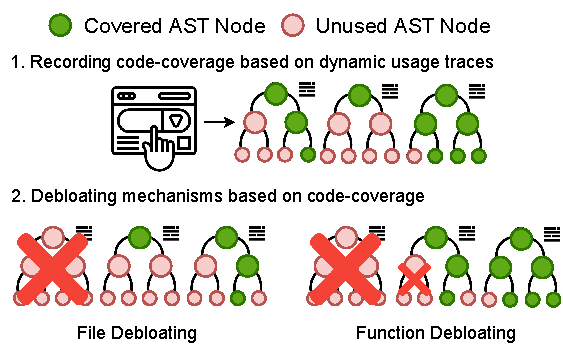
\includegraphics[width=0.75\columnwidth]{figures/dbltr/file_vs_function_debloating.drawio.pdf}
    \caption{File vs Function level debloating based on dynamic code-coverage traces. Root of each AST denotes the entry point of the underlying PHP file. Second layer nodes denote functions, and the leaves are statements inside functions.}
    \label{fig:file_vs_func_debloating}
\end{figure}

\subsection{Debloating based on dynamic usage traces}
Debloating based on dynamic traces for web applications was first introduced in ``Less is More''~\cite{lessismore}, in which we incorporate a set of automation tools and scripts to \emph{simulate} usage behavior while recording the executed server-side files as well as their respective lines.
Figure~\ref{fig:file_vs_func_debloating} represents the two debloating approaches discussed by ``Less is More'' (Chapter~\ref{chap:lim}). 
Based on this code-coverage information (Step 1 in Figure~\ref{fig:file_vs_func_debloating}) ``Less is More'' identifies unused nodes in the Abstract Syntax Tree (AST). 

In ``Less is More'' we discussed two debloating strategies, file-level and function-level debloating. 
In the first approach, file debloating only removes the whole AST of a file, if none of its underlying statements are ever exercised based on the dynamic usage traces. 
Conversely, function debloating is fine-grained and can remove sub-graphs of the AST if it identifies a function with no code-coverage, and therefore, can produce smaller applications with fewer vulnerabilities. 

``Less is More'' incorporates the XDebug PHP module that allows it to record the list of executed PHP file and lines. 
Next step is to configure the web server to start XDebug for each of the running PHP files. 
By configuring XDebug to run for each PHP file invoked by the web server, ``Less is More'' records the list of PHP files and their underlying executed lines and stores them in a database. 
In this work, we follow a similar method to record the code-coverage, and extend ``Less is More'' by looking at \emph{real} user data, and identifying clusters of users that perform similar actions. 

\subsection{Debloating metrics}

Debloating by definition removes or neutralizes parts of the application that users do not require. 
In order to demonstrate the security gains by removing a piece of code, previous work has used several source-code metrics. 

\paragraph{Size reduction} measures how much code was removed through the debloating process. 
McConnell discussed in his work that the size of the code positively correlates with the number of software bugs it contains~\cite{mcconnell2004code}. The reduction in Logical Lines of Code (LLOC) measures the size reduction by counting the number of statements in an application pre-~and post-debloating and is resilient to changes in the syntax and coding style.

\paragraph{Reduction of security vulnerabilities} is another metric that focuses on historic CVEs. 
By mapping public CVEs to the source code of web applications, we can identify whether the vulnerable piece of code is removed by debloating. 
This is a powerful metric as it focuses on real and mostly exploitable vulnerabilities as opposed to proxy variables (such as LLOC) that may or may not result in real vulnerabilities. In terms of downsides, next to the effort required to map vulnerabilities to source code, CVE-reduction is only meaningful in hindsight since it can be used to understand how a debloating system would have performed if an application was debloated \emph{before} the now-known vulnerabilities were discovered. 


\paragraph{Critical API Calls (CAC) reduction} 
PHP applications interact with their environment through the APIs provided by the PHP engine, which are also known as built-in functions. 
These functions expose low-level C API implementations and provide a variety of functionality to perform network, database, and file-system operations. 
Similarly, PHP extensions which are also written in C, expose their functionality through defining new APIs. 

Protecting CACs has received the attention of binary debloating and exploit prevention research in the past. 
Namely, Shredder~\cite{mishra2018shredder}, ROPGuard~\cite{fratric2012ropguard}, and kBouncer~\cite{pappas2012kbouncer} have emphasized the importance of protecting Critical APIs. 
In the realm of web applications, the prior work on taint analysis for vulnerability detection commonly incorporates the list of such critical APIs that attackers can use to execute various types of attacks. 
For instance, attackers can abuse APIs exposed through the MySQLi PHP extension to mount SQL injection attacks. 
Similarly, the exploitation of file-system APIs can lead to arbitrary file-write attacks. 
Therefore, reducing the access of attackers to such functions through debloating provides tangible security benefits. The RIPS tool by Dahse et al. provided a comprehensive list of Critical APIs, which were treated as sinks for PHP taint analysis~\cite{dahse2010rips}. 
We incorporate the 205 sinks from RIPS and measure the removal of such critical API calls (CACs) from the debloated web applications. 

We categorize the sensitive sinks from RIPS into four main groups. \textbf{Code Execution APIs} are those which can be used to directly, or indirectly run code or change the control flow of the application (e.g., call an arbitrary function). 
Next on this list are \textbf{File System APIs} which enable interactions with the file system, such as, deletion and file manipulation and can be abused to take over an application by overwriting files, overriding credentials, and removing sensitive configuration files. 
\textbf{Information Disclosure} functions can be abused by attackers to expose sensitive information from the web application or its host operating system. 
Lastly, for APIs that do not clearly belong to one of the aforementioned categories, we list them under \textbf{Other}. 
This group of critical APIs may allow attackers to conduct malicious actions, such as, sending spam emails, or evading authentication by changing environment variables. 
Next, we look at some examples from each of these categories of critical APIs: 

\begin{itemize}
    \item \textbf{Code Execution APIs:} Consist of OS Shell command execution (e.g., \texttt{exec}, \texttt{passthru}, \texttt{popen}, etc.) PHP code execution (e.g., \texttt{eval}, \texttt{assert}, etc.) and Callbacks (e.g., \texttt{call\_user\_func, array\_map}, etc.)
    \item \textbf{File System APIs :} Consist of functions such as \texttt{fopen}, \texttt{file\_put\_contents}, and \texttt{rename}.
    \item \textbf{Information Disclosure APIs:} Include functions that can leak sensitive information from the web server environment such as \texttt{getenv}, \texttt{get\_current\_user}, and \texttt{phpinfo}.
    \item \textbf{Other APIs:} This group consists of miscellaneous critical APIs such as \texttt{extract}, \texttt{putenv}, \texttt{mail}, etc.
\end{itemize}

The full list of CACs used in this work is available in the Appendix under Table~\ref{tab:cacs}.
    
% \paragraph{PHP Object Injection Gadgets}
% Object injection is a vulnerability where user-controlled values reach an \texttt{unserialize} API without proper sanitization. 
% In such cases, attackers can assemble a list of PHP classes that already exist in an application and mount an exploit which commonly leads to arbitrary file writes and even remote code execution. 

% To understand how attackers exploit PHP object injection vulnerabilities, we need to review two PHP concepts, \emph{Autoloaders} and \emph{Magic functions}. 
% \emph{Autoloading} is a feature in PHP that allows programmers and package developers to register their modules to automatically be loaded by the PHP engine whenever the program instantiates one of their classes. 
% % Therefore, virtually all modern PHP applications that use third-party packages via \texttt{composer} incorporate an autoloader. 
% This expands the ability of the attackers to instantiate all classes across all third-party packages in a vulnerable PHP application. 

% \emph{Magic functions} are special functions that will be invoked automatically by the PHP engine after certain events. 
% Some of the common examples of magic functions used in object injection gadgets are \texttt{\_\_destruct}, \texttt{\_\_toString}, and \texttt{\_\_wakeup}, that are invoked whenever a class is destroyed, converted to a string, or unserialized. 
% % Magic functions sometimes perform sensitive operations, such as, a class destructor performing clean up actions by removing the temporary files generated by that class. 

% In the case of object-injection attacks, the attacker can abuse the code in the existing classes in their target web applications. 
% Since attackers cannot divert the control flow directly by calling arbitrary functions from the injected classes, they rely on specific functions (e.g., class destructors) to piece-together exploit payloads which are called ``gadgets.'' 
% % In the example of destructors removing temporary files, attackers can overwrite the list of these files in the class variable with other sensitive files in the application and force the application to remove them. 

% %Similarly, if the application includes a class with a call to a code execution API (\texttt{include, eval, exec}, etc.) in one of its magic functions, the attackers can abuse this function to run arbitrary code. 

% In this work, we incorporate the list of publicly reported gadgets by PHPGGC~\cite{PHPGGC}. 
% This tool includes a repository of gadget chains within popular third-party packages. 
% Therefore, if a vulnerable application makes use of any of these packages, attackers can inject one of the gadget chains from PHPGGC to gain RCE (Remote Code Execution), write to arbitrary files or interact with the database. 
% PHPGGC does not provide a comprehensive list of gadgets for all packages and all classes in our target web applications. 
% Nevertheless, this approach which is also incorporated in the literature~\cite{lessismore} provides us with a quantitative measure for the reduction in gadget chains after debloating. 

% For each of the web applications in our dataset and their third-party packages, we check for the existence of gadget chains based on the PHPGGC dataset. 
% We then check whether debloating removes these gadgets. 
% For debloated instances where we have removed the gadgets, even if attackers find an object injection vulnerability, they cannot abuse any of the public gadget chains in their exploits. 

% Experimental Design
\section{Experimental Design}

In this section we lay the foundations and discuss the design decisions of our system. 
First we present the details of our user study and data collection. 
We then introduce the design concepts behind \sys{}, our automated pipeline for clustering users into debloating sets and assigning each set to a differently-debloated web application.
Figure~\ref{fig:environment_preparation} shows the high level steps including the data collection and clustering, followed by the preparation of the content delivery environment to serve debloated web applications.

\subsection{User Study - Identifying common web application features from the perspective of experienced administrators}

To understand how experienced users interact with web applications, we conduct the following user study. 
We hire our user-study participants by advertising paid projects on popular freelancing platforms, such as, Upwork~\cite{upwork}. 
After reviewing the resumes and interviewing the candidates, we hire experienced freelancers with 2-10 years of expertise on web development and system administration. 
We specifically interviewed candidates who mentioned phpMyAdmin, WordPress, or Magento on their resume. We focused on these web applications since they were used in the ``Less is More'' study of Amin Azad et al.~\cite{lessismore}, allowing us to compare and contrast our findings with theirs. 

The main goal of this user study is to understand which features in the web applications in our dataset are commonly used among developers and administrators, and which features are relatively unpopular, used by only a fraction of administrators.

\subsubsection{User Study Tasks}

\begin{figure}[t]
    \centering
    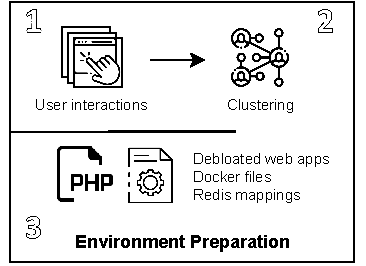
\includegraphics[]{figures/dbltr/EnvironmentPreparation.pdf}
    \caption{During the training phase, we collect user interaction code coverage traces to generate clusters. Based on these clusters, specialized debloated copies of web applications are produced for each cluster.}
    \label{fig:environment_preparation}
\end{figure}

\begin{figure*}[h]
    \centering
    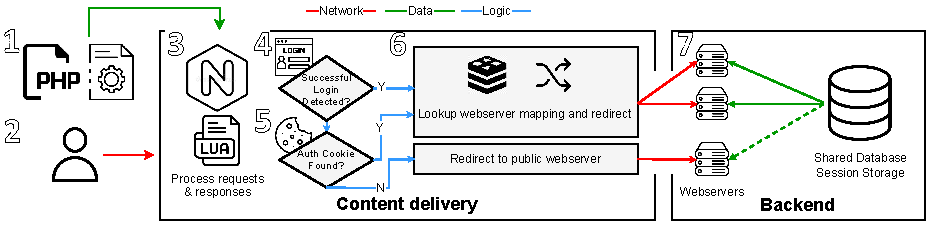
\includegraphics[]{figures/dbltr/RoleModelsFlow.pdf}
    \caption{System Architecture of \sys{}. In Step 1, we provide the debloated web applications and user to cluster mappings to \sys{}'s content delivery module. User requests (2) are processed by \sys{}'s reverse-proxy (Step 3). After identifying the identity of the user (Steps 4-6), \sys{} internally routes the requests to the custom debloated web applications (Step 7).}
	\label{fig:system_architecture}
\end{figure*}

The task description for each project consists of an overview of the user study, the background required to participate, and the expected deliverables. 
Moreover, we included the information about the consent to participate in our study and described the information that we collect (i.e., server-side logs and code-coverage information). 

After interviewing the participants and reviewing their resumes, we hired 20 experts for each web application for a total of 60 experts on phpMyAdmin, WordPress, and Magento. 
We compensate the participants at the rate of \$15 per hour.

During the pilot experiments for the user study, we realized that not every freelancer is familiar with the concept of a user study. 
More importantly, to avoid future disputes, freelancers preferred to work on a predefined list of tasks and deliverables. 

Based on these observations, we defined two milestones for our user study. 
First, we asked our participants to provide a list of web application features that they commonly use in their daily tasks and projects. 
Most of our participants listed both maintenance and administration tasks. 
Among the common tasks, we observed verification of the functionality of the website (e.g., registering as new customers, submitting orders, etc.), maintenance tasks (e.g., backups, import data, etc.) and even search-engine optimization. 

For the second milestone, we asked our participants to spend 1 hour of their time on our instrumented web applications and perform the tasks that they listed earlier. 
This process provided them with the list of deliverables and expectations, and also enabled us to validate their effort on this project. 

For freelancing platforms that provide a time-tracking utility, we use this feature to verify the participation of users together with cross-validating their task report with our code-coverage traces. 
For submissions that did not follow our guidelines (e.g., did not spend enough time, skipped the majority of tasks in the reports, etc.) we would ask the participants to revise their submission. 

\textbf{IRB Approval} Since our experiments involved the assistance of real users, we obtained an Institutional Review Board (IRB) approval for our user study. 
Upon providing thorough details of our tasks and the human interactions, along with the information that we collect from the users, we obtained IRB approval on May 27, 2020. 

\subsubsection{Setup of Web Applications}

To facilitate the setup of web applications for our user study participants, we prepared the following environments:

\begin{itemize}
    \item \textbf{phpMyAdmin:} We provide phpMyAdmin version 5.1.0, with multiple pre-populated databases including a WordPress, and a Magento database.
    \item \textbf{WordPress:} Our setup consists of the version 5.8 of WordPress with an admin account, over 20 blog posts, multiple pages pages, and comments. 
    \item \textbf{Magento:} We setup Magento 2.3.5 and configured the ``Sample data'' package that includes an inventory of over 1,000 products. 
\end{itemize}

Each participant received their own instance with the admin credentials on a unique subdomain. 
We re-create the same environment as ``Less is More'' to collect the usage traces from user interactions in the form of file and line coverage information. 

Through out this user study, we interviewed over 110 individuals, some of whom decided not to participate in our study due to reasons such as non-recurring and short-term nature of our tasks, their busy schedule, etc.
Overall, we spent numerous weeks interviewing our participants and following up with them to ensure the timely delivery of their tasks. The cost of this experiment was approximately \$1,000, most of which was used to pay the administrators in our user study and the remainder to pay for domain names and the hosting of virtual machines on public clouds.

\subsection{Debloating Pipeline}

In this section we describe \sys{}, a dynamic debloating pipeline. 
\sys{} is able to identify web-application users with similar usage profiles (i.e., roles), and create debloated applications that are tailored to the needs of users in each profile. 


Unlike previous one-size-fits-all approaches, application users with specific usage patterns do not need to inherit the whole code-base from other users with vastly different usage behaviors. 
A concrete example of this effect becomes apparent in the usage traces of WordPress. 
Certain administrators focus on the content, and the SEO. 
Therefore, they mostly interact with blog posts and page content, meta tags, and keywords. 
Conversely, another distinct group of administrators focused on changing the appearance of the website by installing new themes, and plugins such as ``Elementor'' that provides an easy interface to modify the appearance of the website. 
In this scenario, by providing the ability to install new plugins to the first group, we are unnecessarily increasing their privileges beyond what they really require. 

For certain web applications, their role-based, access-control mechanisms can limit, to a certain extent, unnecessary capabilities.
Unfortunately many PHP applications that provide administrative features lack this ability (e.g., phpMyAdmin). 
Moreover, the provided roles do not always match the real-world requirements of users. For instance, WordPress comes with only 6 hardcoded roles ranging from Super Admin to Subscriber. 
The benefit of our approach is that we dynamically identify the required web application features based on runtime traces. 

This effect is most significant when applications do not provide fine-grained permission management. 
For instance, using the classic ``single debloated application for all users'' approach, a super admin would share the codebase with data-entry users or even unauthenticated public users. 

Moreover, by clustering users with similar feature usage in the same group, we decrease the likelihood of breaking web application functionality due to removal of code if another user in the same cluster exercised the desired functionality. 
This is in contrast to user-specific debloating where each individual receives their own copy of the target web application based on their exclusive usage patterns. 
We provide a quantitative analysis of this effect in Section~\ref{sec:augmented_coverage}.

\subsubsection{Producing the debloated web applications}

\sys{} extracts the list of exercised files from usage traces. 
PHP file paths and names are effective indicators of the underlying feature corresponding to each file. 
Most commonly, web application source files are partitioned under directories that indicate the feature they implement. 
Moreover, for external dependencies (i.e., composer packages), the file-path includes the name of the module that the files belong to. 

Based on this information, we cluster file paths using the K-means clustering algorithm, into 2 to \emph{N} clusters, with \emph{N} denoting the total number of web application users (in this case, 20).  

\sys{} then produces the following artifacts:
\begin{itemize}
    \item \( \frac{N \times (N - 1)}{2} \) debloated variants of web applications.
    \item Configuration files for the reverse-proxy and the web servers to host the debloated web applications.
    \item Information about the mapping of users to debloating clusters.
\end{itemize}

\subsubsection{Routing users to debloating clusters}

One of the design requirements of \sys{} is seamless user experience. 
Therefore, we incorporate a reverse-proxy that identifies user login information and routes any post-authentication traffic to specialized containers which include debloated variants of the main application customized for the user. 

\sys{}'s reverse-proxy takes a config file for each web application. 
This file informs the proxy of how to identify successful login request-response pairs, the form field that contains the username and the session cookie name to track the user past authentication. 

This information is stored along with the user to web application mappings in an in-memory datastore. 
For authenticated users, the proxy extracts the session cookie, queries the datastore for the web server id for the user and routes the traffic to the appropriate debloated web application. 
From the user's perspective, there is no observable effect while this routing is taking place. Due to the architecture of \sys{}, two users can both be visiting the same URL at the same time, yet accessing radically different (i.e., debloated to match their needs) web applications under the hood. 

\subsubsection{Sharing web application state between web server instances}

Each debloated web application instance is produced from the same source code. 
Nevertheless, the state of each web application depends on the database, cookies, and the session storage. 

In order to keep the state of all web applications synchronized, we connect all of them to the same database instance in the docker environment. 
Moreover, directories that include the session information are mounted as a single volume across all web application instances. 
By sharing this volume, users that authenticate on one copy of the application and are redirected to another debloated instance will maintain their authenticated session cookie. This separation of the session store from web servers is a mainstream principle of scalable web applications allowing requests from the same user to be served by multiple web-server instances~\cite{scalability-book}.
Finally, since web browsers are responsible for maintaining the valid cookies, after routing users to different debloated web application instances served over the same URL, the cookies are automatically transferred along with future requests. 

% Implementation
\section{Implementation}

\dbltr{} consists of multiple data processing, code rewriting, and content delivery steps, making up a full debloating pipeline. 
Initially, our data-analysis step processes the code-coverage traces from web application users and performs the clustering based on the usage data and feature usage. 
Our system incorporates clustering metrics to determine the optimal number of clusters based on code-coverage information, but system operators can decide to modify this configuration based on other post-debloating factors such as LLOC reduction. 

\subsection{Processing the code-coverage information}

For all users of each web application, we extract the list of file and line coverage information. 
Our next task is to identify clusters of code-coverage data based on application usage similarity. 
In order to cluster similar profiles together, we train an unsupervised clustering model based on file names and file paths. 
This decision is based on the intuition that the architecture of popular web applications provides an organic hierarchy of their underlying modules. 

\subsubsection{Vectorizing covered file paths} 
Previously, we argued that file paths and file names are accurate indicators of the underlying feature in the web application based on user interactions and code-coverage traces. 
Based on this observation, we vectorize covered file paths and use TF-IDF algorithm to extract important terms from our corpus of data. 
Throughout this process, we experimentally identified that ignoring common terms that appeared in more than 50\% of the file paths (e.g., \texttt{vendor}, \texttt{wp-admin}, etc.) will yield the best results. 


\subsubsection{Clustering code-coverage information} We use the features returned by the TF-IDF processing in combination with K-Means clustering. 
On one end, we build a single cluster which acts as the baseline for our debloating measurements. 
This cluster which contains the code-coverage of all users resembles the debloating structure of Less is More by Amin Azad et al.~\cite{lessismore}. 
On the other end, we can assign a unique cluster for each user. 
By doing so, each user receives their own uniquely debloated web application which ensures the maximum tailoring of features. 
We argue that the optimal number of clusters lies in between the two extremes, such that the debloating metrics (e.g., code, CVE, and sensitive function call reduction) are optimized while keeping the number of clusters manageable. 

Moreover, as we demonstrate later in Section~\ref{sec:augmented_coverage}, it is beneficial to group users with similar behavior in the same cluster as they will augment each others' code-coverage. 
This aggregation reduces the likelihood of users running into removed features (i.e., features that they did not exercise during the training of the system which were subsequently removed) as other users with similar usage patterns may have already covered the code responsible for the desired feature. 

Web applications sometimes create temporary PHP files for caching purposes. 
Other interactions with the web applications such as installing a new module can also result in the introduction of new PHP code. 
For our debloating scheme, we consider an application at a stable state (i.e., required plugins and modules are already installed prior to debloating). 
Therefore, we perform a cleanup step through which we remove references from code-coverage traces that point to non-existing files in the original version of the applications. 

Our goal in this paper is to demonstrate the debloating performance of popular web applications in their original format. 
Specific to our user study, our cleanup step will essentially remove newly installed modules during the user study experiments, but will keep the code in the original application that enables users to install new modules. 

\begin{figure}[]
    \centering
    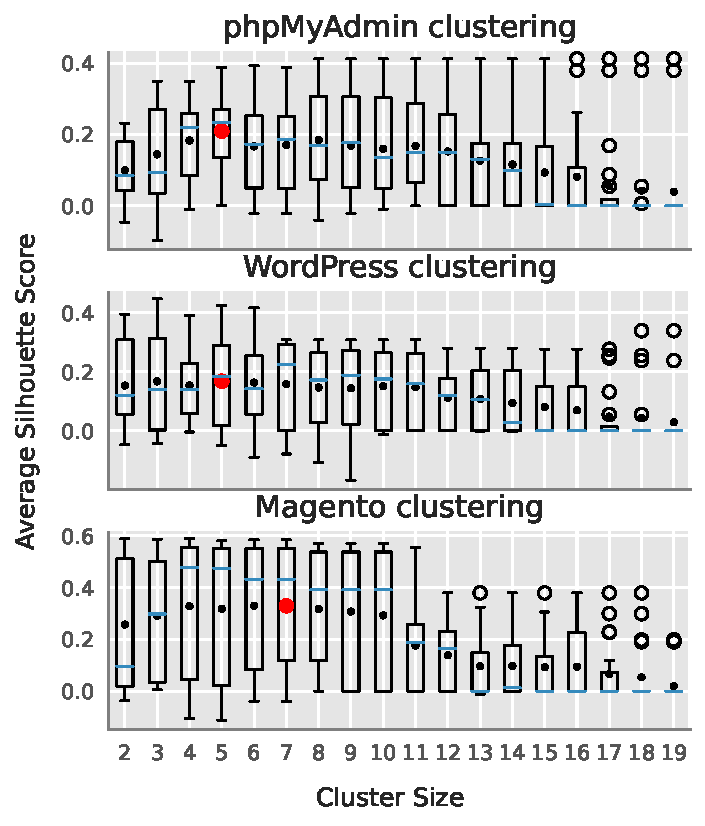
\includegraphics[width=0.50\textwidth]{figures/dbltr/silhouette.pdf}
    \caption{Distribution of Silhouette scores of each cluster. The average score for each cluster is marked with a solid dot and the maximum average is marked with a solid red dot.}
    \label{fig:silhouette_scores}
    \vspace{-1em}
\end{figure}

\subsubsection{Determining the optimal number of clusters} 
\label{sec:num-clusters}

We can determine the optimal number of clusters based on a variety of source code similarity (i.e., file name and path) as well as debloating metrics (i.e., CVE reduction, and CAC reduction). 
\dbltr{} bases its decision on file similarity, concretely file name and path information that is readily available before clustering is performed. 

\dbltr{} then calculates the Silhouette score metric~\cite{kaufman2009finding} for the clusters. 
For each data point, the Silhouette score measures the similarity of the given data point to other points in its own cluster compared to points from other clusters. 
\dbltr{} determines the number of clusters by maximizing the average Silhouette score. 

Figure~\ref{fig:silhouette_scores} depicts the distribution of Silhouette scores based on the cluster size for each of the web applications in our dataset. 
The average score for each cluster size is shown by a solid dot, and optimal cluster size is depicted with a solid red dot. 
Given the ways that the 60 administrators used the evaluated web applications during our user study, the optimal number of clusters are as follows: 5 clusters for phpMyAdmin, 5 for WordPress, and 7 for Magento. 
For certain applications such as Magento, a range of values for the cluster size may be near optimal, in all cases, we selected the number that maximizes the average Silhouette scores.
As the number of clusters increase, we reach an optimal cluster size. 
Beyond this point, by approaching the extreme cluster size (e.g., 19 clusters), we produce many highly-similar small clusters, which reduces the average Silhouette score to close to zero. 

\subsubsection{Debloating the applications} For each cluster, we merge the code-coverage information for all the users of that cluster, and then use the aggregate file and line coverage information to identify unused files and functions and debloat them. 

The process of debloating consists of neutralizing unused files and functions by replacing them with a routine that blocks the further execution of the code. 
This step provides us with \emph{N} copies of the original application, with \emph{N} being the optimal number of clusters determined by \dbltr{}. 
Each debloated cluster caters to the use cases of its underlying users. 
Finally, we calculate the debloating metrics such as size, CVE, and CAC reduction for each cluster. 
We discuss these results in more detail in Section~\ref{sec:debloatingresults}.

\subsection{Content delivery}

The second stage of the \dbltr{} pipeline is responsible for serving the debloated web applications and seamlessly routing users to their underlying debloated web applications. 

\dbltr{} implements a reverse-proxy module based on OpenResty~\cite{openresty}, which is a popular high performance scalable web platform that extends NGINX and provides content manipulation APIs through Lua code. 
This is depicted in Figure~\ref{fig:system_architecture} as step 3. 

We implement the login-detection logic as a Lua module for OpenResty. 
This module is responsible for detecting successful login requests, extracting username and session cookie information, as well as storing and retrieving the user to debloated web application mappings from the data store. 
A high-level representation of the login detection module for phpMyAdmin is depicted in Listing~\ref{lst:lua}.

During the debloating stage, \dbltr{} produces mappings that directs our OpenResty module to redirect users to specific instances of debloated web applications. 
This information is stored in a Redis datastore along with active session-cookie-to-username mappings extracted by the Lua module. 

\definecolor{commentsColor}{rgb}{0.497495, 0.497587, 0.497464}
\begin{lstlisting}[caption=LUA configuration to detect successful logins and extract authentication cookies for phpMyAdmin,label=lst:lua,basicstyle=\footnotesize, float=tp, floatplacement=tbp, language={[5.0]Lua},commentstyle=\color{commentsColor}\textit, numbers=left, xleftmargin=5.0ex, breaklines=true]
-- phpMyAdmin Username extraction
if post_params ~= nil and (string.find(ngx.var.request_uri, "/") or string.find(ngx.var.request_uri, "index.php")) 
  then
    if post_params["pma_username"] ~= nil then
      username = post_params["pma_username"]
    end
end
-- phpMyAdmin Successful login detection
if ngx.var.request_method == "POST" and ngx.var.username ~= "" and ngx.status == 302 then
  -- Successful login detected extract session cookie
  for key, value in pairs(cookies) do
    if string.match(value:lower(), "phpmyadmin") then
      -- Store cookie value in Redis
\end{lstlisting}

For each web application, we provide a configuration file that defines the login endpoint, username form field, and the successful login indicator. 
In the example of phpMyAdmin, successful login is composed of a POST request towards the login endpoint ``/'' or ``index.php'' that receives a 302 HTTP response code which redirects the user to the administration page of the application (Line 2 in Listing~\ref{lst:lua}). 

We extract the username from the POST request with the field name of ``pma\_username'' (Line 4) 
and then verify through the HTTP response code that we detected a successful login (Line 9). Finally, we extract the session cookie named ``phpmyadmin'' (Line 12) and store this user-to-session-cookie mapping in the Redis data store for subsequent requests. 

For subsequent requests containing a valid session cookie, \dbltr{} first queries the username from the data store and then determines the target web server based on the username mapping. 
Steps 4, 5, and 6 in Figure~\ref{fig:system_architecture} depict this process. 
Once the upstream web server is determined, traffic is routed to the corresponding web server. 
Any subsequent log-out requests and timeouts invalidate the session-cookie mapping.
% Debloating Results
\definecolor{commentsColor}{rgb}{0.497495, 0.497587, 0.497464}
\begin{lstlisting}[belowskip=-1em, caption=LUA configuration to detect successful logins and extract authentication cookies for phpMyAdmin,label=lst:lua,basicstyle=\footnotesize, language={[5.0]Lua},commentstyle=\color{commentsColor}\textit, numbers=left, xleftmargin=5.0ex, breaklines=true, float=t, floatplacement=t]
-- phpMyAdmin Username extraction
if post_params ~= nil and (string.find(ngx.var.request_uri, "/") or string.find(ngx.var.request_uri, "index.php")) 
then
    if post_params["pma_username"] ~= nil then
    username = post_params["pma_username"]
    end
end
-- phpMyAdmin Successful login detection
if ngx.var.request_method == "POST" and ngx.var.username ~= "" and ngx.status == 302 then
-- Successful login detected extract session cookie
for key, value in pairs(cookies) do
    if string.match(value:lower(), "phpmyadmin") then
    -- Store cookie value in Redis
\end{lstlisting}

\section{Debloating Results}
\label{sec:debloatingresults}

In this section, we measure the debloating performance of our system and demonstrate its ability to reduce the attack surface of web applications beyond the previous work. 
Next, we compare the debloating results of \dbltr{} and quantify its improvements over the baseline model through source code metrics such as LLOC reduction, as well as security metrics, namely CVE, gadget chain, and CAC reductions. 
% Historically, research papers demonstrated the attack-surface reduction of debloating schemes via the reduction in size of debloated applications.
% Other studies report the removal of historic CVEs and gadget chains as a means to measure the security gains of debloated applications. 
% We extend the existing metrics by measuring and reporting the number of calls to critical API.

% \subsection{Clustering Statistics}
% During our data collection step, we collected the code-coverage data from web application usage from 20 experts for each web application.
% We then clustered their code-coverage information into 1-20 clusters. 
% On one end, the code-coverage information from all users are aggregated in a single cluster. 
% On the other end, all users have their own uniquely debloated web applications that contain only the code that they have interacted with before. 
% While \dbltr{} is capable of providing uniquely debloated web applications for each user, it is beneficial to keep the number of clusters low in order to reduce the complexity of separately maintaining $N$ applications. 

% \subsubsection{Characterizations of \dbltr{} clustering}
% For \dbltr{} debloating clusters, we look at statistics such as number of users in each cluster, as well as the high level roles of each cluster. 

% For the web applications in our dataset, we observe a common list of tasks that are shared among the majority of users. 
% For phpMyAdmin, virtually all users created new database and tables, executed SQL queries, and used the functionality of exporting and importing the database.
% Some users also renamed or modified existing databases, dropped tables, or deleted rows of data. 
% For WordPress, setting up themes and installing custom plugins, and creating new blog posts were among the commonly used features. 
% Finally, for Magento, creating new products, managing product inventory, and modifying prices were the most popular features. 

% \begin{figure}[t]
%     \centering
%     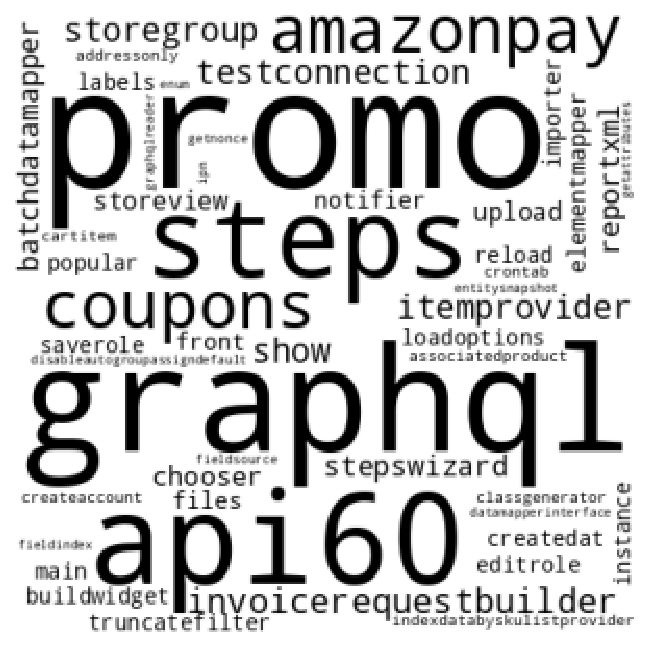
\includegraphics[width=0.5\textwidth]{figures/dbltr/magento_wordcloud.pdf}
%     \caption{Word cloud of important terms for Magento cluster number four}
%     \label{fig:magento_wordcloud}
% \end{figure}

% On the other hand, we observe patterns of feature usage that are unique to a subset of users. 
% Among these user-specific features we observe exporting files with specific file extensions (e.g., CSV), using filters while displaying the query results, and modifying privileges. 
% Similarly, Import/Export, modifying settings such as permalinks, RSS, and WXR are unique to certain clusters among the WordPress users. 
% Finally, for Magento, sales promotions, gifts and shopping cart rules, front end content modification, and sales analytics are among the unique features. 

% We incorporate this observation into our clustering via the max-document-frequency parameter in TF-IDF. 
% This way, we can ignore the common features that are used across all clusters and focus on the unique features when building the clusters. 

% At this step, by looking at the most important terms for each cluster, we can assign a role title to the users of the cluster. 
% Figure~\ref{fig:magento_wordcloud} depicts the word cloud of important terms for a sample cluster of administrators in Magento. 
% Larger font size indicates a higher impact factor based on TF-IDF metric. In general, by analyzing the output of TF-IDF, we can define the following roles for clusters:

% \begin{itemize}
%     \item Mass actions (Delete, Copy, Refresh).
%     \item Invoice, PDF, and Less files.
%     \item Payment methods, Gift cards, and Refunds.
%     \item APIs (GraphQL, XML), Promo, Coupons.
%     \item Index, Cache, Internationalization (i18n).
%     \item Cart, Suggestions, Recommendations.
%     \item Guest purchases, Compare products, Shipping.
% \end{itemize}

\subsection{Debloating results}
%By definition, debloating reduces the effective size of web applications. 
%In this section, we discuss the results of LLOC (Logical Lines of Code), CVE, and CAC (Critical API Call) reduction.

\subsubsection{LLOC Reduction}
 
We measure the reduction in size of web applications in terms of logical lines of code (LLOC), which counts the number of statements in the application source code. 
By reporting the size of the debloated applications in LLOC, we reduce the effects of various syntax and coding styles (i.e., the debloating process changing the code style after rewriting). 

Table~\ref{tab:lloc_reduction} shows the LLOC reduction results of our debloating scheme. 
The numbers are reported in terms of thousands of LLOC. 
The column marked as ``Baseline'' lists the debloating results of combining the code-coverage data of all users together and assigning them to a single role, which is equivalent to prior debloating approaches, such as the one by ``Less is More'' of Amin Azad et al.~\cite{lessismore}.
``\dbltr{}'' shows the LLOC statistics with the optimal number of roles chosen by \dbltr{} for each web application, as discussed in Section~\ref{sec:num-clusters}. 
For \dbltr{} column, we report the size of the role with highest debloated LLOC (Max) and the smallest role with minimum removed LLOC (Min) along with the median. 
The number in the parenthesis for Baseline and \dbltr{} denotes the percentage of LLOC reduction with respect to the size of the original application. 

By comparing the LLOC reduction of Baseline to \dbltr{}, it becomes evident that a one-size-fits-all debloating (i.e., Baseline), exposes certain users and roles to a much larger code-base than they actually require. 
This unnecessary bloat for Baseline debloating can be as high as 30\% of extra LLOC for applications.  
%Nick: This feels like a repetition
%By contrasting the minimum and maximum reduction in \dbltr{} roles, it is evident that in one-size-fits-all debloating schemes certain users would be exposed to a much larger code base than they actually need. 
This unnecessary exposure is most significant for larger web applications such as Magento where certain users inherit up to 90,000 unnecessary LLOC which is 36\% larger---compared to the smallest \dbltr{} role---than what they actually need. 

Moreover, we observe that \emph{all} \dbltr{} roles (including the one with maximum remaining LLOCs) are strictly smaller than the Baseline, meaning that the globally debloated application is still bloated as far as individual users are concerned. 

\begin{table}[t]
    \caption{LLOC reduction of debloated clusters: Numbers are reported in terms of thousands of LLOC. For Baseline, and \dbltr{}, we report the percentage of LLOC reduction compared to the Original application. \dbltr{} columns show the roles with maximum, median and minimum  number of debloated LLOC.}
    \centering
    \adjustbox{max width=\linewidth}{
        \begin{tabular}{|l|l|l|lll|}
            \hline
            \multirow{2}{*}{\textbf{\begin{tabular}[c]{@{}l@{}}Web\\ Application\end{tabular}}} & \multirow{2}{*}{\textbf{Original}} & \multirow{2}{*}{\textbf{Baseline}} & \multicolumn{3}{c|}{\textbf{DBLTR}}                                                  \\ \cline{4-6} 
                                                                                    &                                    &                                    & \multicolumn{1}{l|}{\textbf{Max}} & \multicolumn{1}{l|}{\textbf{Median}} & \textbf{Min} \\ \hline
                phpMyAdmin                                                                          & 155                                & 44 ($\blacktriangledown$72\%)                          & \multicolumn{1}{l|}{32 ($\blacktriangledown$79\%)}    & \multicolumn{1}{l|}{39 ($\blacktriangledown$75\%)}     & 42 ($\blacktriangledown$73\%)     \\ \hline
                WordPress                                                                           & 103                                & 66 ($\blacktriangledown$36\%)                          & \multicolumn{1}{l|}{44 ($\blacktriangledown$57\%)}    & \multicolumn{1}{l|}{54 ($\blacktriangledown$48\%)}    & 64 ($\blacktriangledown$38\%)     \\ \hline
                Magento                                                                             & 1,050                              & 330 ($\blacktriangledown$69\%)                         & \multicolumn{1}{l|}{240 ($\blacktriangledown$77\%)}   & \multicolumn{1}{l|}{270 ($\blacktriangledown$74\%)}   & 326 ($\blacktriangledown$69\%)   \\ \hline
        \end{tabular}
    }
    \label{tab:lloc_reduction}
\end{table}

By comparing the LLOC reduction of Baseline to \dbltr{}, it becomes evident that a one-size-fits-all debloating (i.e., Baseline), exposes certain users and roles to a much larger code-base than they actually require. 
This unnecessary bloat for Baseline debloating can be as high as 30\% of extra LLOC. 
This unnecessary exposure is most significant for larger web applications such as Magento where certain users inherit up to 90,000 unnecessary LLOC which is 37\% larger---compared to the smallest \dbltr{} cluster---than what they actually need. 
Moreover, we observe that \emph{all} \dbltr{} clusters (including the one with maximum LLOCs) are strictly smaller than the Baseline approach, meaning that the globally debloated web application is still bloated as far as individual users are concerned.

\subsubsection{CVE Reduction}

One of the metrics to model the effects of debloating on the security of applications is removal of actual vulnerabilities. 
Historic CVEs provide a good source of information on vulnerabilities and we incorporate a mapping of CVE to source code to identify whether a debloated variant of applications includes the vulnerability or not. 

One of the challenges of this approach is the availability of patch information. 
In order to map a CVE to the vulnerable parts of the source code, we use the data that is available in the form of bug report analysis, Git diffs, and security patches. 
The goal of this step is to identify the files and functions responsible for the vulnerability. 

In our user study, we focused on the latest versions of web applications, so we opted to map all CVEs to these versions. 
In practice, this translates to mapping the location of a CVE to a specific function in a specific file, even if that function is currently patched. 
The purpose of this step is to identify whether the code that contained the vulnerability would have been retained by a debloating approach because it was part of the functionality that the administrators in our user study relied upon.

Some of the web applications in our dataset maintained a stable structure of their source code over time (e.g., WordPress) which makes the process of mapping CVEs from older versions to the recent one straightforward. 
Conversely, phpMyAdmin and Magento changed drastically since their older versions (i.e., Magento version 1.x vs 2.x) and it is not always possible to find the same PHP file/class to perform the mapping. 
Moreover, the developers of phpMyAdmin and WordPress usually acknowledge CVEs in their patches and GitHub commits, whereas for Magento, CVEs are only discussed with minimal details and the patches are released in the form of Major and Minor updates ranging from 500 to 4,000 modifications.

As a result, we mapped 20 CVEs to the source code of phpMyAdmin and WordPress, and mapped 10 recent CVEs to source code of Magento, for a total of 50 mapped CVEs. 
We selected the CVEs with the highest CVSS score, and skipped the ones where the vulnerability or patch information was unavailable. 
The full list of the 50 CVEs that we used in our study along with the information about the \dbltr{} roles such as the number of roles and users that are exposed to each CVE after debloating is available in Table~\ref{tab:cve_details} in the Appendix. 

\begin{figure}[t]
    \centering
    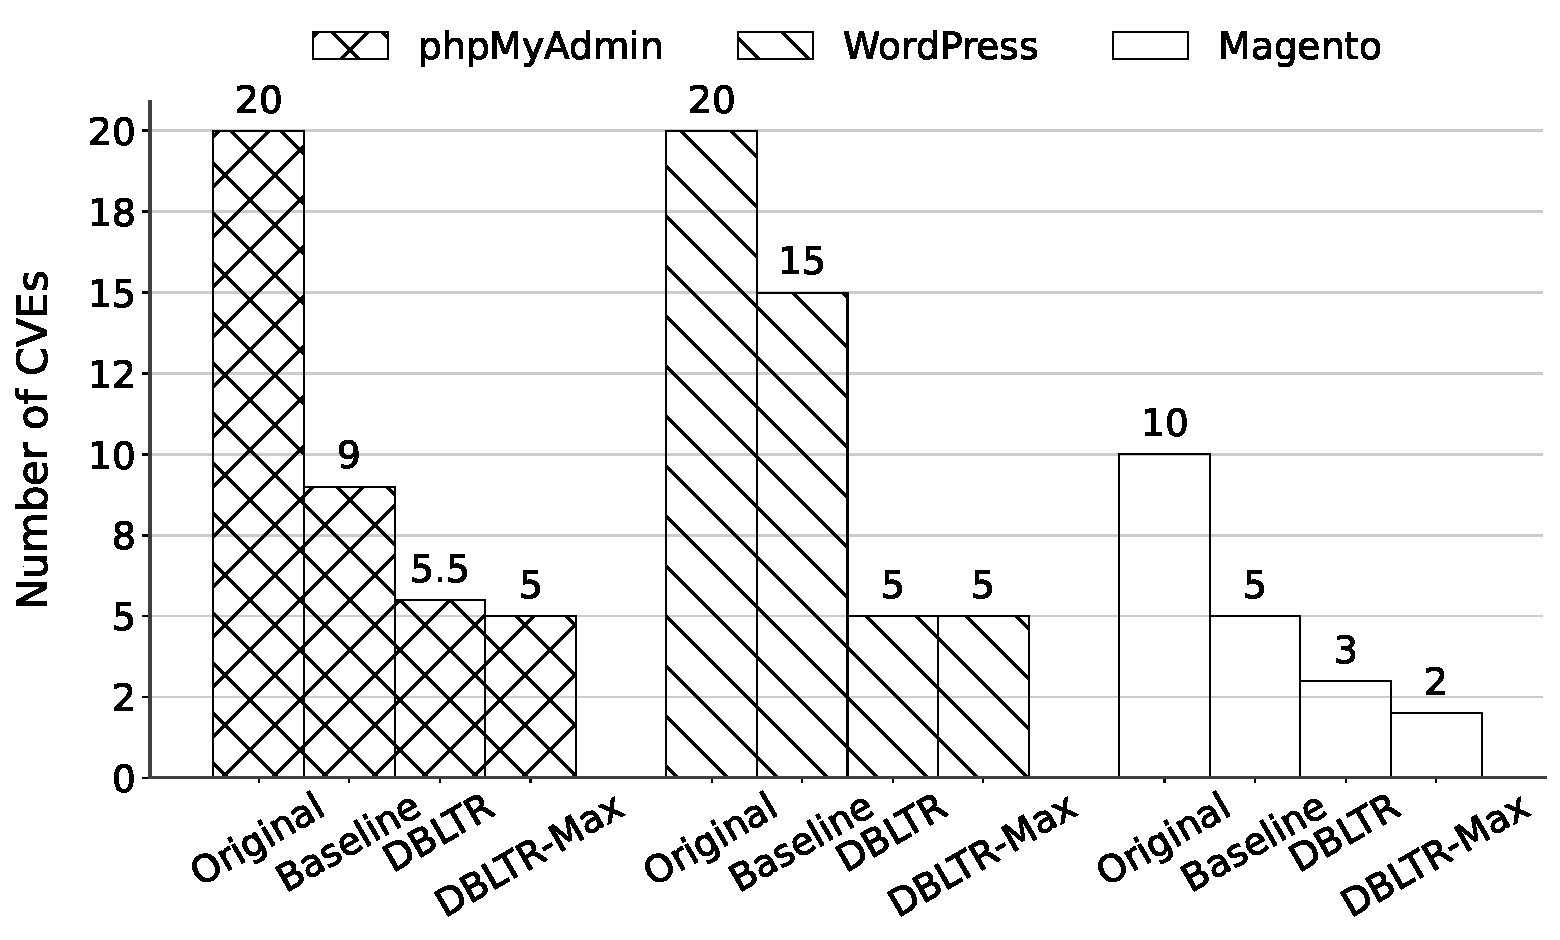
\includegraphics[width=\linewidth]{figures/dbltr/cve_reduction_spectral_bw.pdf}
    \caption{CVE reduction statistics of debloated web applications. ``Original'' represents the total number of mapped CVEs, ``Baseline'' represents the reduction of global debloating, ``DBLTR'' depicts the median reduction across roles, and ``DBLTR-Max'' represents the roles with the highest CVE reduction.}
    \label{fig:cve_reduction}
\end{figure}

Figure~\ref{fig:cve_reduction} depicts the number of CVEs remaining after debloating for each web application. 
The ``\dbltr{}'' bar shows the median CVE reduction across roles, while ``\dbltr{}-Max'' shows the roles with highest CVE reduction representing the maximum protection provided by \dbltr{} for users in those roles. 
For example, for phpMyAdmin we discover that 3/6 roles (accounting for 65\% of users) exposed to the fewest remaining vulnerabilities. 
These roles contained 5 historic CVEs corresponding to 45\% reduction of CVEs compared to the Baseline debloating and 75\% reduction compared to the non-debloated application. 
Similarly, the median number of vulnerabilities among the roles was 5.5 accounting for 40\% reduction compared to the Baseline approach. 
This effect is even more pronounced in WordPress where \dbltr{} reduces the median number of CVEs per role to 4 accounting for a 73\% reduction compared to the 15 CVEs remaining after the Baseline debloating approach. 
Magento exhibits a similar trend of localized debloating gains.

Overall, our results demonstrate that debloating web applications based on clusters of usage-data (i.e., roles) results in significant reduction of severe historic CVEs, compared to prior debloating schemes that could only remove code that was determined to be globally unnecessary for all users of a deployed web application.

\subsubsection{Case Study: phpMyAdmin Database Export Local file Inclusion Vulnerability}

phpMyAdmin version 4.0 is vulnerable to CVE-2013-3240 which resides in the database export functionality. 
This vulnerability allows the attackers to bypass the \texttt{checkParameters} function by sending a specially-crafted variable. 
phpMyAdmin uses this variable to determine the database export file type (e.g., .sql, or .zip) and load the corresponding plugin. 
Malicious users can abuse this flaw to load and execute arbitrary PHP files from the server. 

The export feature in phpMyAdmin is commonly used to backup existing databases and therefore is highly unlikely to be removed by prior global-debloating mechanisms.
Nevertheless, we observed that one of our roles produced by \dbltr{} included four users who did not exercise the export functionality. As a result, \dbltr{} is able to remove this feature from the source code of that specific role, protecting the web application from abuse by these four specific users (including from attackers who compromise their accounts). 

\begin{figure}[t]
    \centering
    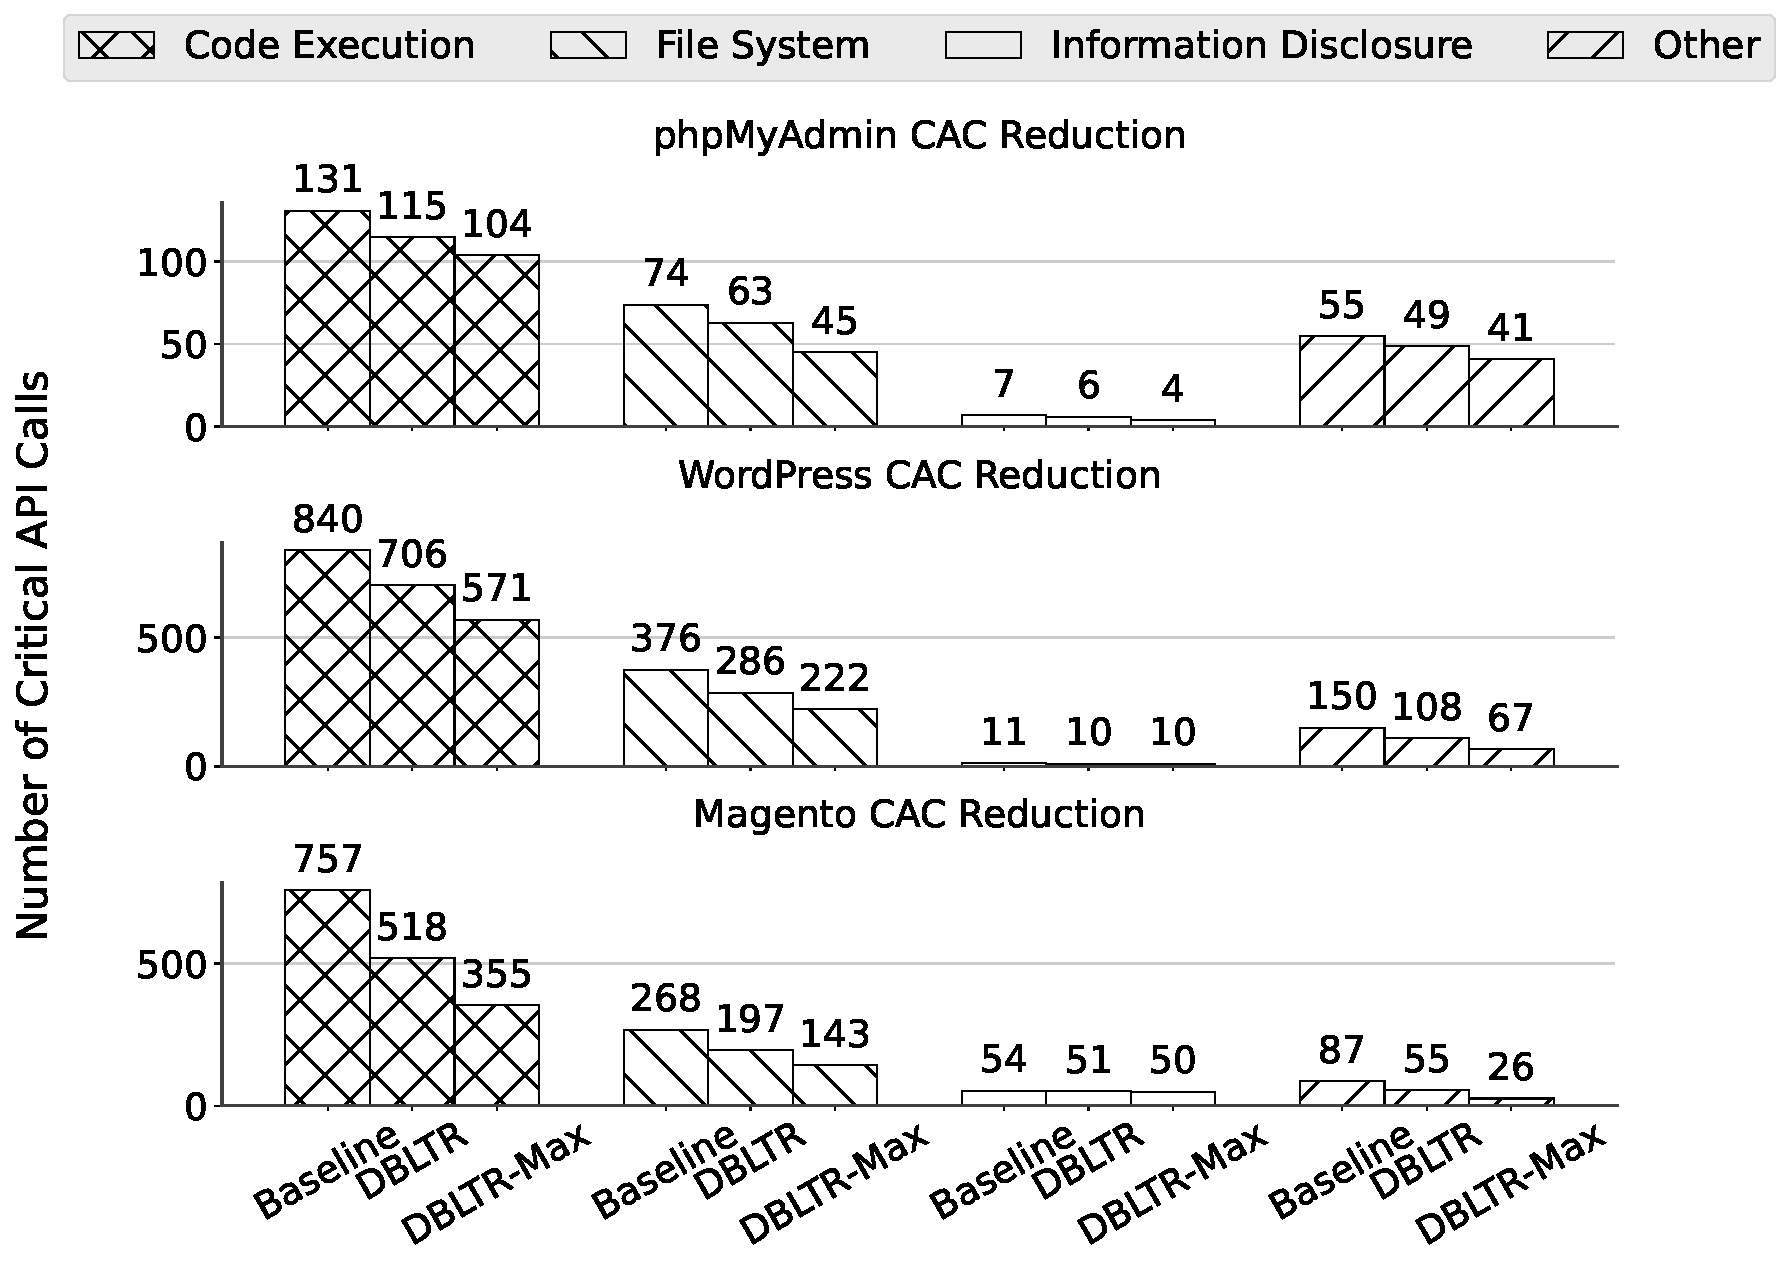
\includegraphics[width=\linewidth]{figures/dbltr/cac_reduction_spectral_bw.pdf}
    \caption{Critical API Call (CAC) reduction after debloating. Baseline represents the global debloating approach where all users are assigned to the same role. \dbltr{} indicates the average reduction across roles.}
    \label{fig:cac_reduction}
\end{figure}

\subsubsection{Critical API Calls Reduction}

Another security metric that we analyze is the reduction in Critical API Calls (CACs). 
Figure~\ref{fig:cac_reduction} depicts the average CAC reduction across all roles. 
The first bar of each group shows the total number of CACs for the Baseline debloating. 
Baseline indicates the reductions in the global debloating scheme where all users are grouped into a single role. 
\dbltr{} bars show the average reduction of CACs based on the optimal number of roles for each web application and \dbltr{}-Max represents the maximum reduction in CACs for a subset of users. 

Across all CAC categories and all web applications, we observe a reduction of 10\% up to 70\% for \dbltr{} debloating. 
This reduction indicates that a sizable number of CACs are in unused parts of the applications. Upon closer inspection of phpMyAdmin results, it becomes evident that 85\% of code execution APIs reside in the external dependencies of the web application, out of which, \dbltr{} removed 12\%-20\%. 
For the larger applications such as Magento, the reduction in Code Execution APIs is more significant where 32\%-53\% of these APIs are removed by \dbltr{}.
Over all categories of CACs, we observe that \dbltr{} removes tens to hundreds of such API calls beyond the Baseline, further protecting web applications from exploits that target these APIs. 

\begin{table}[t]
    \centering
    \caption{PHP Object Injection Gadgets statistics after debloating. Listing number of existing gadgets for Baseline and the percentage of roles in \dbltr{} exposed to those gadgets.}
    \label{tab:poi_gadgets}
    \scalebox{1}{
        \begin{tabular}{|l|l|c|c|c|}
            \hline
            Web Application             & Package & Original & Baseline & \dbltr{} \\ \hline
            \multirow{2}{*}{phpMyAdmin} & Symfony & 2        & 0        & 0     \\ \cline{2-5} 
                                        & TCPDF   & 1        & 1        & 83\%  \\ \hline
            WordPress                   & Generic & 1        & 0        & 0     \\ \hline
            \multirow{3}{*}{Magento}    & Guzzle  & 3        & 2        & 100\%, 0\% \\ \cline{2-5} 
                                        & Magento & 1        & 1        & 14\%  \\ \cline{2-5} 
                                        & Monolog & 6        & 0        & 0     \\ \hline
            \end{tabular}
    }
\end{table}

\subsubsection{PHP Object Injection Gadget Reduction}

To identify existing object injection gadgets in the applications, we incorporate PHPGGC~\cite{PHPGGC}, an open-source project listing available gadget chains for popular composer packages. 
After mapping the list of vulnerable package with those in phpMyAdmin, WordPress, and Magento, we search for the removal of classes and functions used within the gadget chains after debloating. 

Table~\ref{tab:poi_gadgets} lists the packages in each of our web applications with a known gadget chain based on PHPGGC. 
Under the column named ``Original'' we list the number of gadget chains within each package. 
As before, the Baseline column lists the number of gadget chains available after the global debloating (i.e., single role), whereas the \dbltr{} column lists the percentage of roles in \dbltr{} exposed to these gadgets. 

The Symfony package in phpMyAdmin includes 2 known gadget chains that can lead to arbitrary file write and code execution. 
Debloating the application into 1-Cluster (Baseline) as well as \dbltr{} debloating remove these gadgets. 
For TCPDF gadget, while the baseline debloating does not remove it, \dbltr{} protects 17\% of the clusters from object injection exploits using this gadget. 
For WordPress, the baseline debloating strategy removes the existing gadget therefore there are no opportunities for any additional gains by \dbltr{}.

More interestingly, Magento contains 10 known gadget chains. 
For Magento's Guzzle package, we observe that while 2 gadgets are still present in the Baseline debloating, one of the gadget chains is fully removed from all roles.
For the gadget chain within the Magento package itself, only (1/7) 14\% of roles produced by the \dbltr{} contain this gadget, therefore, the majority of users are protected.

Our results confirm the findings of previous work that debloating is a highly effective defense for removing publicly known object injection gadget chains. 
Moreover, we observe that by clustering users into multiple groups, we can further breakdown the availability of gadgets and in certain cases, further complicating the exploitation of object injection vulnerabilities. Under a \dbltr{}-protected deployment, attackers not only need to identify the available gadgets in the target web application to build their exploit chain, but they also have to target \emph{specific} victims who have access to the underlying gadgets used in their exploits. 

% \subsection{Contribution of individual users to the overall code-coverage of clusters}
% \label{sec:augmented_coverage}

% Dynamic code-coverage data precisely models how users interact with web applications. 
% One of the limitations of this modeling is that it overlooks the use cases that it has not seen before. 
% As an example in our dataset, we observed that certain users executed queries that resulted only in a few rows. 
% Therefore, some of the functions within the ``Display Results'' class of phpMyAdmin relating to pagination of results were never invoked. 
% Meanwhile, other users with very similar usage behavior that ended up in the same cluster executed queries that exercised the pagination functions. 
% As a result, all users within this cluster would retain this functionality and can run queries that result in numerous rows.
% In such scenarios, the clustering expands the available features for users with similar usage patterns. 

% To quantify this effect, we look at the contribution of individual users in the cluster compared to the overall cluster code-coverage. 
% For each user, we compare their file and function coverage information with all other users in the same cluster. 
% To identify similar functionality that have been added to the cluster coverage by other users, we look at new lines covered in an already covered file. 
% This modeling captures the effect of exercising new features within an already covered file.
% Moreover, we investigate the inclusion of new files in the overall coverage within an existing module. 
% For this purpose, we closely investigate the source code structure of the web applications in our dataset and identify the directory structure of their internal and external (e.g., composer) packages. 

% \subsubsection{Analyzing module structures} By analyzing the code-base structure of the applications in our dataset, we made the following observations:

% \textbf{phpMyAdmin} uses composer packages. As a result, external dependencies such as Twig, Symfony, Tcpdf, etc. are located under \texttt{vendor/package\_author/package\_name/} directory structure.
% Similarly, phpMyAdmin stores internal modules and classes such as Charsets, Display, Export, etc. under \texttt{libraries/classes/module\_name/}. 
% For phpMyAdmin, we identified 98 external and 23 internal modules.

% \textbf{WordPress} unlike phpMyAdmin, does not use external composer packages. 
% Nevertheless, WordPress modules are split into public and admin sections. 
% Admin modules are located under \texttt{wp-admin/includes/class\_name} and public modules are under \texttt{wp-includes/class\_name}. 
% Some examples of these modules are, PHPMailer, Requests, Rest-API, Widgets, etc.
% Similarly, WordPress themes and plugins have their own unique directory under \texttt{wp-content/themes} and \texttt{wp-content/plugins} directory. 
% For WordPress we identified 23 first-party modules. 

% \textbf{Magento} incorporates multiple first-party and third-party modules via composer. 
% Also, internal modules and classes are located under \texttt{app/code/Magento/module\_name} as well as \texttt{generated/code/module\_name}. 
% From the Magento source code, we identified 493 external and 190 internal modules. 

% Statistics on the code-coverage contribution of clusters to each individual user are available in Table~\ref{tab:augmented_coverage}. 
% Under the column ``\% Files with new coverage'' we report the percentage of total files for which the cluster contributed new lines to the code-coverage of each individual member of that cluster. 
% This number ranges from 15.3\% to 38.3\%, which signifies that a considerable number of functions for each class are included in the final code-coverage by other users in the same cluster. 

% Table~\ref{tab:augmented_coverage} also lists the total number of third-party packages and first-party class modules. 
% Clustering led to inclusion of new files for an average of 29\% to 71\% of packages, and 50\% to 72\% of class modules. 
% On a similar note, these results quantitatively demonstrate that clustering users with similar behavior together leads to inclusion of similar functions, and therefore, reduces the likelihood of removing functions that are actually required by the users. 
% Users who make extensive use of the necessary web-application features cluster together with users with more lightweight usage, allowing the latter to gradually expand their use without breaking the web application due to debloated code. 

% Finally, we look at the number of ``Removed Packages'' for the clusters produced by \dbltr{} in Table~\ref{tab:augmented_coverage}. 
% This column reports the number of packages in the web application where a given percentage of lines are removed after debloating.
% These statistics show that for over half of the packages for phpMyAdmin and Magento, debloating has removed more than 70\% of their lines. 
% In other words, while clustering users with similar behavior together expands their code-coverage of similar features significantly, the debloating procedure is still successfully removing the majority of the code from third-party dependencies, where majority of the bloated code resides~\cite{lessismore}.

\subsection{Performance of \dbltr{}}

We analyze the performance of \dbltr{} from two perspectives, request response time, and server resource utilization. 
Our test setup consists of an HTTP client and the web server. 
The HTTP clients simulate 100 users that send requests in parallel. 
Each client runs in a separate thread and sends batches of 40 requests (average number of requests to load the homepage of WordPress and its resources) towards the main page of WordPress hosted on a remote server. 
This setup simulates the work load for a website with 192,000 daily page views receiving 90 requests-per-second. 
We run each test for five minutes and repeat the tests five times and report the average statistics and remove the outliers. 

For the server setup, our web server hosts a WordPress website and we run each configuration in a containerized environment. 
We run our web servers on a server with 32GBs of RAM, and 32 Cores of Intel Xeon E5-2440 v2 CPUs running Ubuntu 18.04 LTS. 
We test the following setups:

\begin{itemize}
    \item \textbf{Single web server (Apache)} consists of one Apache web server without a reverse-proxy. 
    \item \textbf{Baseline} is made up of an OpenResty reverse proxy and one Apache web server. This setup serves as our baseline. 
    \item \textbf{\dbltr{} setups} expand the baseline setup by including the \dbltr{} modules and consist of one reverse-proxy and 1-50 Apache web servers. Each web server is responsible for the debloated web application for a specific role. This way, we measure the effect of the number of roles on the request response times. Under this setup, each client is assigned to one role in a round-robin fashion.
\end{itemize}

\begin{figure}[]
    \centering
    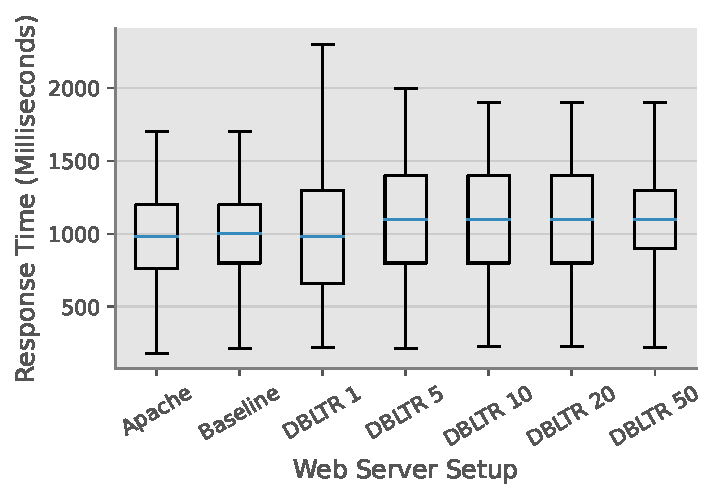
\includegraphics[width=0.8\linewidth]{figures/dbltr/performance.pdf}
    \caption{Distribution of request response time in milliseconds for Apache, Baseline, and \dbltr{} with a varying number of roles (i.e., backed Apache servers).}
    \label{fig:performance}
  \end{figure}

\subsubsection{Request Response Time Statistics}
We measure the request response time statistics from the perspective of our HTTP clients and report them in Figure~\ref{fig:performance}. 
The mere addition of the reverse-proxy (Baseline) increases the median response time of requests by 2\%. 
For \dbltr{}, the overhead from analysis and routing modules results in an average increase of 12\% in the median response time and 15\% increase in the 99th percentile response time. 
Moreover, a higher number of roles reduces the variance in the response times, as evident by the smaller boxes and shorter whiskers from one (DBLTR 1) to fifty roles (DBLTR 50). 

\subsubsection{Resource Utilization}
We measured the CPU and memory utilization of our test setup using the Docker runtime metrics API. 
Table~\ref{tab:performance} reports the resource usage statistics for the web servers and content-delivery (i.e., reverse-proxy) modules. 
Overall, the content-delivery module both in baseline and \dbltr{} setups utilizes 5-6\% of CPU and less than 20~MiB of RAM which is very small compared to the amount of resources utilized by the web server. 
Moreover, across all setups, the CPU utilization of the web server modules remains constant. 
At the same time, increasing the number of roles in \dbltr{} which results in an increase in the number of web servers results in a linear increase in the overall memory utilization. 
During our tests, we observed a 5x increase in overall memory usage of \dbltr{}'s web servers when increasing the number of roles by an order of 50x. 

\paragraph{Disk space utilization} \dbltr{} stores a separate and unique debloated copy of the web applications for each role. 
As a result, the disk utilization overhead of \dbltr{} is proportional to the number of roles. 
While shrinking the disk utilization of \dbltr{} is not a main goal, by definition, the debloating process removes unused lines of code. 
Overall, debloated web applications occupy 5-10\% less disk space. 
While this reduction may be insignificant for smaller web applications, for larger ones such as Magento, debloated web applications on average occupy 100~MB less disk space. 


\begin{table}[]
    \centering
    \caption{Average CPU and Memory utilization of \dbltr{}. \textit{DBLTR N}-Web Servers row shows the range of CPU and Memory utilization for \textit{DBLTR 1} to \textit{DBLTR 50}.}
    \label{tab:performance}
    \adjustbox{max width=\columnwidth}{
    \begin{tabular}{|l|l|l|l|}
    \hline
    \textbf{Setup}                    & \textbf{Module}  & \textbf{Avg CPU} & \textbf{Avg Memory (MiB)} \\ \hline
    Apache                            & Web Server       & 3,117\%              & 2,378                            \\ \hline
    \multirow{2}{*}{Baseline}         & Content-Delivery & 6\%                 & 17                           \\ \cline{2-4} 
                                      & Web Server       & 3057\%              & 2,332                         \\ \hline
    \multirow{2}{*}{\textit{DBLTR N}} & Content-Delivery & 6\%                 & 19                           \\ \cline{2-4} 
                                      & Web Servers      & 2,905-3,072\%      & 2,179-10,374                \\ \hline
    \end{tabular}
    }
\end{table}
% Discussion
\section{Discussion}

In this section we discuss and evaluate possible strategies for handling the addition and removal of users from a \dbltr{}-protected web application. We then review the important takeaways, and finally discuss the limitations of our approach.

\subsection{Addition and Removal of Users} 

The process of assigning a role to new users in RBAC web applications is based on an administrator's discretion regarding the required capabilities of the new users. 
Unlike traditional RBAC roles, \dbltr{} roles are defined dynamically and are unique to each deployment of a web application based on the behavior of its users. 
As a result, assigning new users to existing \dbltr{} roles requires special treatment. 

The conservative approach is to assign new users to a non-debloated web application and record their usage behavior. \dbltr{} can straightforwardly handle this by the mere introduction of a new containerized environment containing that non-debloated web application and a mapping rule assigning the new user to that container. A more aggressive approach is to assign users to a \emph{globally-debloated} web application with the expectation that a newly added user will use features used by at least one existing user of that web application. For both strategies (i.e., conservative and aggressive assignment), administrators can collect usage traces for that new user and eventually invoke \dbltr{} to produce new roles and migrate the new user to a more tailored cluster of users.

To evaluate the latter more aggressive user-assignment strategy, we start by assuming a setup for \dbltr{} where the usage traces for the majority of users have been collected and the roles are produced. This setup resembles an environment (e.g., a company) where the majority of employees were present for the usage-trace collection period and a limited number of new users (e.g., newly-hired employees) are periodically added to this steady-state system. When a new user is added to the system, we use the sum of the code-coverage of all existing users to produce a globally-debloated web application, which still contains a significantly smaller attack-surface compared to the original application. 


To simulate this, we conduct the following leave-one-out experiment: we remove the code-coverage information of each user from the training dataset and create a debloated copy of the web application based on the code-coverage of remaining users (i.e., 19/20 users). 
This globally-debloated web application is strictly larger than any of the role-specific copies of the same application and is equivalent to prior dynamic debloating approaches~\cite{lessismore}. We then simulate the addition of new users by introducing the code-coverage of the user that we left out and measuring false positives, i.e., the files required by that user that are not present in the globally-debloated web application.

\begin{figure}[t]
    \centering
    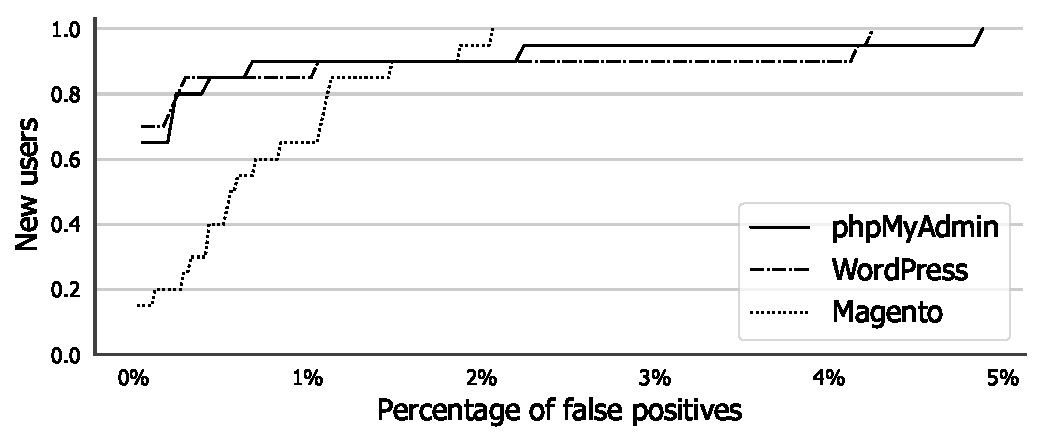
\includegraphics[width=\linewidth]{figures/dbltr/cdf_falsepositives_bw.pdf}
    \caption{CDF of observed false positives from the perspective of new users. The X axis depicts the percentage of false positives (i.e., ratio of the number of missing files compared to total used files by each new user).}
    \label{fig:adding_new_users}
\end{figure}

Figure~\ref{fig:adding_new_users} provides the CDF of false positives (i.e., missing files) when adding new users. 
For phpMyAdmin and WordPress, the majority (60-70\%) of users in the leave-one-out experiment could be added to the ``globally-debloated'' web application without any false positives. 
Likewise, more than 85\% of new users would experience breakage in less than 1\% of the overall files that they interact with. 
For Magento, while most new users assigned to the ``globally-debloated'' web application would experience some breakage, most still fall below the 1\% threshold. 
Overall, across all three web applications in our dataset, even for users with notably unique behavior, we observe less than 5\% of the overall files missing when their usage behavior traces were omitted from the training dataset. 

Looking at the unique behavior of users that led to false positives, in phpMyAdmin, we observe enabling multistep authentication modules, using query explainer features, and creating SQL Views to be the underlying cause (i.e., desired functionality that is unavailable to new users). For WordPress, customizing the RSS feed, using specific text blocks in posts such as text art, and quotes, and using less popular embedding protocols led to false positives under this aggressive user-assignment strategy. Finally, for Magento, various users interacted with unique features.  These features include third-party integrations (e.g., monitoring, marketing, and automation services), PDF invoices, and wish lists. 

Overall, our results show that the modular architecture of \dbltr{} allows it to successfully serve different types of environments. For environments with fixed workloads or where security is prioritized over usability, \dbltr{} can be used to assign new users to a globally-debloated web application. Alternatively, when administrators are unsure about the needs of new users, \dbltr{} can be used to serve the original version of a web application to these users, until enough usage traces are collected to allow \dbltr{} to create new roles and clusters. In either scenario, the security-related debloating benefits of existing users are not in any way compromised when new users are added to a system. In terms of removing users, administrators can merely disable user-role mappings in \dbltr{}'s configurations and optionally delete containers that do not have any roles associated with them.

\subsection{Main Takeaways}

\noindent\textbf{Static roles in web applications are over authorized and administrators only need a subset of the available features:} 
Throughout our user study, we determined that administrators of the same web application use different subsets of the features available to them. 
While in theory, administrators have full access to every feature in the administration panel, in practice only 25\% and 52\% of the lines in the administrative panels of phpMyAdmin and WordPress respectively, were among the commonly exercised features. 
Evidently, the existing authorization mechanisms of these applications aim to offer access to a large variety of features whereas, in reality, administrators only need a subset of them. 
\dbltr{} builds an accurate list of required features and enforces the principle of least privilege via debloating. 

\noindent\textbf{One-size-fits-all debloating still produces bloated web applications:} 
As demonstrated by this work and the literature, debloating web applications is highly effective in reducing the attack-surface of web applications by removing unused features and their underlying vulnerabilities. 

The global debloating approach explored by the prior work produces one debloated web application which as demonstrated by our analysis, can contain as much as 29\% extra LLOC compared to what users actually need. 
In this work, we integrated \dbltr{} with a dynamic debloating scheme and demonstrated that \dbltr{} can provide improvements across all debloating metrics. 
We demonstrated that in the case of global debloating, users in at least half of the roles would be provided with larger web applications containing 5,000-60,000 more lines of code than required, and exposed to 40\%-70\% more CVEs.

% \noindent\textbf{Clustering users with similar behavior together reduces the likelihood of broken features:} 
% In Table~\ref{tab:augmented_coverage} we reported that 15-38\% of files covered by each user in a cluster had new functions covered by other users in the same cluster. 
% Moreover, 29-71\% of third-party packages in a cluster and more than half of internal modules had new files added to the coverage from the perspective of each member of the clusters. 
% Both of these results show that clustering users based on their feature usage can produce debloated applications with shrunk attack-surface, while reducing the likelihood of debloating useful features due to overfitting to the specific usage traces of individual users. 

\noindent\textbf{\dbltr{} provides a content delivery environment for debloated web applications:} 
One of the main contributions of our work is our content delivery pipeline which reduces the need for modifications and customizations to target web applications, while keeping the debloating platform entirely invisible to web application users.

\subsection{Limitations} 

%Our work comes with some limitations that we discuss in this section. 

\noindent\textbf{Debloating statistics: }
As part of our analysis on the security benefits of debloating, we mapped 50 CVEs to the source code of our applications. 
We used recent versions of three popular web applications for our user study and debloating.
By the time they become public, CVEs are either already patched or will be patched soon. 
Therefore, we mapped historic CVEs to the patched functions within the new web applications. 
As a result, our reports on CVE reduction indicate the removal of a feature in a more recent version of web application compared to the original version that included the actual vulnerability. This was a ``necessary evil'' since we could not rely on users perfectly replicating their workloads across multiple versions of the same web applications where the original vulnerabilities resided.

\noindent\textbf{Usage behavior modeling: }
Our debloating reports are based on the code-coverage that we collected during our user study. Using our domain knowledge, we have established that the collected dataset is a representative sample of web-application use in the real world. At the same time, different deployments of web applications may be used differently and therefore be debloated differently. Regardless of the degree of use, \dbltr{} can offer concrete security advantages to any existing or future end-to-end debloating strategy by automatically removing code that is not globally required by all users of a given deployment and clustering users to their appropriately-debloated codebase.

\noindent\textbf{Applications with a public interface: }
As depicted in Figure~\ref{fig:system_architecture}, \dbltr{} routes unauthenticated requests towards a ``public'' profile of the debloated web application. 
This profile includes the code for user authentication as well as any other code required for public unauthenticated users. 

For administrative applications that are behind an authentication wall, producing a public profile is straightforward. 
In the example of phpMyAdmin, we only need to perform successful and failed login attempts to generate the baseline code-coverage and debloat the application to produce the public debloated profile. 
For other applications such as WordPress and Magento, this step is more involved. 
First, we would remove all the files that are only available to the administrators, for the WordPress and Magento, this constitutes of removing administrator directories (e.g., \emph{wp-admin} for WordPress and \emph{module-backend} directory for Magento).
Next, we need to only retain the features and modules that are available to public users. 
Therefore, we need to record the code-coverage of unauthenticated users with benign behavior. 

One of the main benefits of our role-based debloating is the removal of features that are not limited by the authentication and authorization boundaries of web applications. 
If attackers can somehow taint the code-coverage of unauthenticated profiles to include a vulnerable piece of code, they can force the debloating pipeline to retain that code, and exploit it later. This only applies to the potential vulnerabilities in the public interface of the applications. 
A possible solution to this problem is to use artificial modeling techniques, such as automated crawlers, to extract the code-coverage of public users. 

\noindent\textbf{Changes to the source code:} 
In this work, we studied the debloating of web applications at a stable state. 
That is, all the required configurations, updates, and plugins were installed and available at the time of debloating. 
For smaller updates, we need to repeat the debloating to produce new copies of the updated web application while not touching the modified files during the update. 
For major version updates that include drastic changes to the architecture of the source code and modules, we would need to collect the code-coverage traces again. This limitation is shared by all debloating systems that offer security benefits via late-stage code transformations. Note however that \dbltr{} can be used to stage a move from the old version of a web application to the new version by slowly migrating users from their old containerized environments to the new ones, one role at a time.

\noindent\textbf{Number of users of the web applications:} 
In our user study, we hired a total of 60 participants (20 participants for each web application). 
While most websites are operated by a small number of administrators, there clearly exist web applications (such as popular social networks) with billions of users and thousands of administrators. Understanding how \dbltr{} could be used in such an environment requires the collaboration of a large operator, something which we do not have access to. \dbltr{}'s current architecture does allow for horizontal scaling of servers, enabling it to serve an arbitrary number of users and roles. As such, we hope that, through the open-sourcing of our system, large organizations will be able to evaluate \dbltr{} in their environments and user populations.
% Related Work
% \section{Related Work} 
The idea of software debloating was initially discussed by Zeller et al.~\cite{zeller2002simplifying} as a means to isolate failure-inducing code. 
This idea was later applied to the context of software security to reduce the attack surface of applications. 
Ghavamnia et al. and Rastogi et al. explored the idea of debloating containers~\cite{rastogi2017cimplifier, 259711}, while Abubakar et al. debloated the kernel~\cite{abubakar2021shard}. 
Orthogonally, another line of research explores binary debloating~\cite{snyder2017most, redini2019b, heo2018effective, quach2018debloating, qian2020slimium, ghavamnia2020temporal, mishra2020saffire, koo2019configuration}, and debloating web applications~\cite{lessismore, saphire, mininode, jahanshahi2020you}. 

At a high level, there are three mainstream approaches to debloating: 
i) using static analysis to identify unreachable code~\cite{redini2019b, snyder2017most, quach2018debloating, mininode, 255308}, ii) 
debloating reachable code which is unused given a set of tests (e.g., automated test cases, or dynamic code-coverage traces)~\cite{lessismore, heo2018effective,qian2020slimium, koo2019configuration}, and finally, iii) API specialization, which consists of disabling sensitive APIs or hardening them with respect to the execution context of applications~\cite{mishra2020saffire, saphire, jahanshahi2020you, mishra2021sgxpecial}. 

Our work is mainly motivated by the ``Less is More'' approach of Amin Azad et al.~\cite{lessismore}. By comparing the debloating results of \sys{} with the baseline debloating approach of ``Less is More'' (Section~\ref{sec:debloatingresults}), we demonstrated that role-based debloating outperforms the ``Less is More'' approach, both in terms of security metrics, as well as on reducing concrete vulnerabilities. 

In another line of work targeting binaries and web applications, Mishra et al.~\cite{mishra2018shredder, mishra2021sgxpecial}, Bulekov et al.~\cite{saphire}, and Jahanshahi et al.~\cite{jahanshahi2020you} provided solutions to reduce the software attack surface of applications through limiting the list of available APIs for each piece of code. 
By incorporating their defense, attackers are limited in their ability to exploit the application vulnerabilities. 
These solutions are orthogonal to our work and can be used in combination with \sys{} to further protect the applications against the exploitation of potential vulnerabilities. 

Koishybayev et al. proposed Mininode, a tool to reduce the attack surface of Node.js applications by debloating third-party modules~\cite{mininode}. 
Their approach is based on static analysis which they use to identify unreachable code in third-party modules and the chain dependencies of Node.js applications. 
While static analysis is helpful in identifying unused code, several categories of common web application vulnerabilities (e.g., SQLi, XSS, CSRF, etc.) reside in reachable parts of the source code. 
\sys{} incorporates dynamic analysis and therefore, is capable of debloating even the reachable but unused parts of the code. 

Bocic et al. and Son et al. studied access-control bugs in web applications~\cite{7582754, son2013fix}. 
They analyzed access-control flaws in Ruby on Rails and PHP applications and identified over 100 authorization bugs in the existing open-source applications. Their findings reinforce the motivation for \sys{}'s role-based debloating which can guarantee the separation of public vs. authenticated users, even in the presence of access-control errors.
% Conclusion
\section{Conclusion}

In this paper, we explored the idea of ``role-based debloating'', which consists of producing multiple versions of debloated web applications, each tailored to a cluster of users with similar usage behaviors (i.e., roles). 
We started by conducting a user study to understand how experienced developers and administrators interact with web applications. 
We then used this data in combination with \sys{}, our proposed tool that is capable of collecting code-coverage traces of the users of an application, to form clusters of users with similar usage behavior, and produce debloated applications customized to the needs of each cluster. 
\sys{} also includes a content-delivery pipeline that can transparently route users to their clusters of dedicated debloated web applications without the need to modify the target web applications. 

Through our detailed analysis, we quantitatively showed that \sys{} can outperform the state-of-the-art in web application debloating. 
By incorporating the idea of role-based debloating, we can produce debloated web applications that are 30\% smaller in size, and contain 80\% fewer severe vulnerabilities (i.e., historic CVEs) compared to the ``globally'' debloated web applications produced by prior work. We also explored the contribution of each user to the code-coverage of clusters, in an effort to understand the robustness of clustered debloating compared to the extreme where each users receives their own copy of the debloated applications. 

We showed that \sys{}'s clustering expands the code-coverage of similar features in each cluster for up to 38\% of all files, which affects more than half of the packages and classes in the web applications. This effect on the code-coverage allows \sys{} to retain the code for similar features that cluster members may use in future. 
Overall, our results indicate that role-based debloating is a practical approach with tangible security benefits, and should be considered as a means to protect security-critical web applications. 


%Acknowledgements
%First and foremost, I would like to express my deepest appreciation to my advisor, Nick Nikiforakis. 
I learned a lot from his work ethics and wisdom, and benefited from his support through all these years. 
I would also like to express my gratitude to R Sekar, Michalis Polychronakis, Manuel Egele, and Adam Doupé for serving on my dissertation committee and providing me with helpful feedback. 
 
During my Ph.D journey, I was honored to work with great researchers whom I learned a lot from. Above all, I am sincerely grateful to Pierre Laperdrix for his professional attitude, his humor, and his endless support and motivation. 
I enjoyed every moment of working with my colleagues and collaborators, Rasoul Jahanshahi, Chris Tsoukaladelis, Oleksii Starov, Najmeh Miramirkhani, Xigao Li, Brian Kondracki, Tim Barron, Meng Luo, Johnny So, Billy Tsouvalas, and Mohammad Muzammil. 

None of this would have been possible without the love and encouragement of my family, Zohre, Masoud, Mamani, Shahnaz, and Behnam. 
Special thanks to Hooman the cat, for being of no help at all. 
Thanks should also go to my friends who were there for me, Mina, Javad, Reza, and the Iranian community. 
I owe my professional career in cybersecurity to Mohammad Jorjandi, my mentor, who always had my personal growth in mind and set me on this path, 7,000 miles away from home. 
Lastly, thanks to Alyssa, for her unconditional love and support. 
% Availability
\section{Availability}

To ensure full transparency while promoting future work in the space of debloating web applications, we will provide public access to \emph{all} developed code and artifacts upon publication of this paper.

% \section{Appendix}

\begin{table}[]
    \caption{List of CVEs and statistics of affected clusters and users after debloating.}
    \label{tab:cve_details}
    \centering
    \begin{adjustbox}{max width=0.65\textwidth}
    \begin{tabular}{|lllll|}
    \hline
    % phpMyAdmin CVEs
    \multicolumn{5}{|c|}{\textbf{phpMyAdmin}}                                                                                                                                                                                                 \\ \hline
    \multicolumn{1}{|l|}{\multirow{2}{*}{\textbf{\#}}} & \multicolumn{1}{l|}{\multirow{2}{*}{\textbf{CVE}}} & \multicolumn{2}{l|}{\textbf{Percentage of Affected}}                         & \multirow{2}{*}{\textbf{Affected Functionality}} \\ \cline{3-4}
    \multicolumn{1}{|l|}{}            & \multicolumn{1}{l|}{}                 & \multicolumn{1}{l|}{\textbf{Clusters}} & \multicolumn{1}{l|}{\textbf{Users}} &                                 \\ \hline
    \multicolumn{1}{|l|}{1}           & \multicolumn{1}{l|}{CVE-2020-26935}   & \multicolumn{1}{l|}{0\%}                  & \multicolumn{1}{l|}{0\%}               & SQLi in SearchController        \\ \hline
    \multicolumn{1}{|l|}{2}           & \multicolumn{1}{l|}{CVE-2020-26934}   & \multicolumn{1}{l|}{0\%}                  & \multicolumn{1}{l|}{0\%}               & XSS in Table Transformation     \\ \hline
    \multicolumn{1}{|l|}{3}           & \multicolumn{1}{l|}{CVE-2020-10802}   & \multicolumn{1}{l|}{0\%}                  & \multicolumn{1}{l|}{0\%}               & SQLi in search action           \\ \hline
    \multicolumn{1}{|l|}{4}           & \multicolumn{1}{l|}{CVE-2020-10804}   & \multicolumn{1}{l|}{0\%}                  & \multicolumn{1}{l|}{0\%}               & SQLi in username                \\ \hline
    \multicolumn{1}{|l|}{5}           & \multicolumn{1}{l|}{CVE-2020-5504}    & \multicolumn{1}{l|}{20\%}                 & \multicolumn{1}{l|}{15\%}              & SQLi in user accounts page      \\ \hline
    \multicolumn{1}{|l|}{6}           & \multicolumn{1}{l|}{CVE-2019-6798}    & \multicolumn{1}{l|}{40\%}                 & \multicolumn{1}{l|}{25\%}              & SQLi in username                \\ \hline
    \multicolumn{1}{|l|}{7}           & \multicolumn{1}{l|}{CVE-2019-12616}   & \multicolumn{1}{l|}{100\%}                & \multicolumn{1}{l|}{100\%}             & CSRF to run arbitrary queries   \\ \hline
    \multicolumn{1}{|l|}{8}           & \multicolumn{1}{l|}{CVE-2018-12613}   & \multicolumn{1}{l|}{0\%}                  & \multicolumn{1}{l|}{0\%}               & RCE in page load module         \\ \hline
    \multicolumn{1}{|l|}{9}           & \multicolumn{1}{l|}{CVE-2017-1000499} & \multicolumn{1}{l|}{100\%}                & \multicolumn{1}{l|}{100\%}             & CSRF to delete tables \& rows   \\ \hline
    \multicolumn{1}{|l|}{10}          & \multicolumn{1}{l|}{CVE-2017-1000017} & \multicolumn{1}{l|}{20\%}                 & \multicolumn{1}{l|}{15\%}              & Authorization bypass            \\ \hline
    \multicolumn{1}{|l|}{11}          & \multicolumn{1}{l|}{CVE-2016-5734}    & \multicolumn{1}{l|}{0\%}                  & \multicolumn{1}{l|}{0\%}               & RCE in table search \& replace  \\ \hline
    \multicolumn{1}{|l|}{12}          & \multicolumn{1}{l|}{CVE-2016-6616}    & \multicolumn{1}{l|}{40\%}                 & \multicolumn{1}{l|}{25\%}              & SQLi in user group \& designer  \\ \hline
    \multicolumn{1}{|l|}{13}          & \multicolumn{1}{l|}{CVE-2016-5703}    & \multicolumn{1}{l|}{0\%}                  & \multicolumn{1}{l|}{0\%}               & SQLi in central columns         \\ \hline
    \multicolumn{1}{|l|}{14}          & \multicolumn{1}{l|}{CVE-2016-6606}    & \multicolumn{1}{l|}{100\%}                & \multicolumn{1}{l|}{100\%}             & Crypto vulnerability in cookies \\ \hline
    \multicolumn{1}{|l|}{15}          & \multicolumn{1}{l|}{CVE-2016-9849}    & \multicolumn{1}{l|}{100\%}                & \multicolumn{1}{l|}{100\%}             & Root restriction bypass         \\ \hline
    \multicolumn{1}{|l|}{16}          & \multicolumn{1}{l|}{CVE-2016-6633}    & \multicolumn{1}{l|}{0\%}                  & \multicolumn{1}{l|}{0\%}               & RCE in dBase extension          \\ \hline
    \multicolumn{1}{|l|}{17}          & \multicolumn{1}{l|}{CVE-2016-6609}    & \multicolumn{1}{l|}{0\%}                  & \multicolumn{1}{l|}{0\%}               & RCE in array export             \\ \hline
    \multicolumn{1}{|l|}{18}          & \multicolumn{1}{l|}{CVE-2016-6619}    & \multicolumn{1}{l|}{0\%}                  & \multicolumn{1}{l|}{0\%}               & SQLi against control user       \\ \hline
    \multicolumn{1}{|l|}{19}          & \multicolumn{1}{l|}{CVE-2014-8959}    & \multicolumn{1}{l|}{0\%}                  & \multicolumn{1}{l|}{0\%}               & Directory traversal in GIS      \\ \hline
    \multicolumn{1}{|l|}{20}          & \multicolumn{1}{l|}{CVE-2013-3240}    & \multicolumn{1}{l|}{80\%}                 & \multicolumn{1}{l|}{80\%}              & RCE in export format            \\ \hline
    % WordPress CVEs
    \multicolumn{5}{|c|}{\textbf{WordPress}}                                                                                                                                                                 \\ \hline
    \multicolumn{1}{|l|}{1}           & \multicolumn{1}{l|}{CVE-2018-12895}   & \multicolumn{1}{l|}{0\%}                  & \multicolumn{1}{l|}{0\%}               & RCE in posts page                       \\ \hline
    \multicolumn{1}{|l|}{2}           & \multicolumn{1}{l|}{CVE-2018-10101}   & \multicolumn{1}{l|}{20\%}                 & \multicolumn{1}{l|}{15\%}              & URL validator bypass                    \\ \hline
    \multicolumn{1}{|l|}{3}           & \multicolumn{1}{l|}{CVE-2018-10100}   & \multicolumn{1}{l|}{100\%}                & \multicolumn{1}{l|}{100\%}             & Open redirect in login page             \\ \hline
    \multicolumn{1}{|l|}{4}           & \multicolumn{1}{l|}{CVE-2017-5611}    & \multicolumn{1}{l|}{20\%}                 & \multicolumn{1}{l|}{15\%}              & SQLi in WP\_Query                       \\ \hline
    \multicolumn{1}{|l|}{5}           & \multicolumn{1}{l|}{CVE-2017-14723}   & \multicolumn{1}{l|}{20\%}                 & \multicolumn{1}{l|}{15\%}              & SQLi in prepare query                   \\ \hline
    \multicolumn{1}{|l|}{6}           & \multicolumn{1}{l|}{CVE-2017-16510}   & \multicolumn{1}{l|}{20\%}                 & \multicolumn{1}{l|}{15\%}              & SQLi in double prepare                  \\ \hline
    \multicolumn{1}{|l|}{7}           & \multicolumn{1}{l|}{CVE-2017-5492}    & \multicolumn{1}{l|}{20\%}                 & \multicolumn{1}{l|}{15\%}              & CSRF in widget accessibility mode       \\ \hline
    \multicolumn{1}{|l|}{8}           & \multicolumn{1}{l|}{CVE-2017-9064}    & \multicolumn{1}{l|}{100\%}                & \multicolumn{1}{l|}{100\%}             & CSRF in filesystem credentials dialog   \\ \hline
    \multicolumn{1}{|l|}{9}           & \multicolumn{1}{l|}{CVE-2017-17091}   & \multicolumn{1}{l|}{60\%}                 & \multicolumn{1}{l|}{40\%}              & Access restriction bypass               \\ \hline
    \multicolumn{1}{|l|}{10}          & \multicolumn{1}{l|}{CVE-2017-6815}    & \multicolumn{1}{l|}{20\%}                 & \multicolumn{1}{l|}{15\%}              & Open redirect in plugins interface      \\ \hline
    \multicolumn{1}{|l|}{11}          & \multicolumn{1}{l|}{CVE-2016-6635}    & \multicolumn{1}{l|}{0\%}                  & \multicolumn{1}{l|}{0\%}               & CSRF in AJAX compression                \\ \hline
    \multicolumn{1}{|l|}{12}          & \multicolumn{1}{l|}{CVE-2016-7169}    & \multicolumn{1}{l|}{0\%}                  & \multicolumn{1}{l|}{0\%}               & Directory traversal in file upload      \\ \hline
    \multicolumn{1}{|l|}{13}          & \multicolumn{1}{l|}{CVE-2015-2213}    & \multicolumn{1}{l|}{0\%}                  & \multicolumn{1}{l|}{0\%}               & SQLi in un-trash comments               \\ \hline
    \multicolumn{1}{|l|}{14}          & \multicolumn{1}{l|}{CVE-2015-5731}    & \multicolumn{1}{l|}{20\%}                 & \multicolumn{1}{l|}{15\%}              & CSRF in edit posts                      \\ \hline
    \multicolumn{1}{|l|}{15}          & \multicolumn{1}{l|}{CVE-2014-5203}    & \multicolumn{1}{l|}{0\%}                  & \multicolumn{1}{l|}{0\%}               & RCE in customize widgets                \\ \hline
    \multicolumn{1}{|l|}{16}          & \multicolumn{1}{l|}{CVE-2014-5204}    & \multicolumn{1}{l|}{20\%}                 & \multicolumn{1}{l|}{15\%}              & CSRF in plugins interface               \\ \hline
    \multicolumn{1}{|l|}{17}          & \multicolumn{1}{l|}{CVE-2014-5205}    & \multicolumn{1}{l|}{0\%}                  & \multicolumn{1}{l|}{0\%}               & CSRF in plugins interface               \\ \hline
    \multicolumn{1}{|l|}{18}          & \multicolumn{1}{l|}{CVE-2014-9033}    & \multicolumn{1}{l|}{100\%}                & \multicolumn{1}{l|}{100\%}             & CSRF in reset password                  \\ \hline
    \multicolumn{1}{|l|}{19}          & \multicolumn{1}{l|}{CVE-2014-9037}    & \multicolumn{1}{l|}{20\%}                 & \multicolumn{1}{l|}{15\%}              & Authentication bypass                   \\ \hline
    \multicolumn{1}{|l|}{20}          & \multicolumn{1}{l|}{CVE-2014-9038}    & \multicolumn{1}{l|}{20\%}                 & \multicolumn{1}{l|}{15\%}              & SSRF in HTTP module                     \\ \hline
    % Magento
    \multicolumn{5}{|c|}{\textbf{Magento}}                                                                                                                                                                   \\ \hline
    \multicolumn{1}{|l|}{1}           & \multicolumn{1}{l|}{CVE-2020-9689}   & \multicolumn{1}{l|}{0\%}                   & \multicolumn{1}{l|}{0\%}               & RCE in WYSIWYG                           \\ \hline
    \multicolumn{1}{|l|}{2}           & \multicolumn{1}{l|}{CVE-2019-7877}   & \multicolumn{1}{l|}{0\%}                   & \multicolumn{1}{l|}{0\%}               & XSS in manage orders                     \\ \hline
    \multicolumn{1}{|l|}{3}           & \multicolumn{1}{l|}{CVE-2019-7139}   & \multicolumn{1}{l|}{100\%}                 & \multicolumn{1}{l|}{100\%}             & Unauthenticated SQLi                     \\ \hline
    \multicolumn{1}{|l|}{4}           & \multicolumn{1}{l|}{CVE-2019-8144}   & \multicolumn{1}{l|}{100\%}                 & \multicolumn{1}{l|}{100\%}             & RCE in page builder                      \\ \hline
    \multicolumn{1}{|l|}{5}           & \multicolumn{1}{l|}{CVE-2019-7877}   & \multicolumn{1}{l|}{0\%}                   & \multicolumn{1}{l|}{0\%}               & Stored XSS in admin panel                \\ \hline
    \multicolumn{1}{|l|}{6}           & \multicolumn{1}{l|}{CVE-2019-8118}   & \multicolumn{1}{l|}{29\%}                  & \multicolumn{1}{l|}{15\%}              & Weak crypto in customer login            \\ \hline
    \multicolumn{1}{|l|}{7}           & \multicolumn{1}{l|}{CVE-2019-8141}   & \multicolumn{1}{l|}{29\%}                  & \multicolumn{1}{l|}{50\%}              & RCE in import functionality              \\ \hline
    \multicolumn{1}{|l|}{8}           & \multicolumn{1}{l|}{CVE-2018-5301}   & \multicolumn{1}{l|}{0\%}                   & \multicolumn{1}{l|}{0\%}               & CSRF in delete address                   \\ \hline
    \multicolumn{1}{|l|}{9}           & \multicolumn{1}{l|}{CVE-2016-6485}   & \multicolumn{1}{l|}{0\%}                   & \multicolumn{1}{l|}{0\%}               & Weak random generator in crypto module   \\ \hline
    \multicolumn{1}{|l|}{10}          & \multicolumn{1}{l|}{CVE-2016-4010}   & \multicolumn{1}{l|}{43\%}                  & \multicolumn{1}{l|}{6\%}               & RCE in shopping cart                     \\ \hline
    \end{tabular}
    \end{adjustbox}
    \end{table}

\begin{table}[t]
\caption{List of Critical PHP APIs}
\label{tab:cacs}
\begin{adjustbox}{max width=\textwidth}
\begin{tabular}{|l|p{20cm}|}
\hline
    \textbf{Category}               & \textbf{Critical APIs} \\ \hline 
    \textbf{Command Execution} & \texttt{exec, passthru,
    system, shell\_exec, popen, proc\_open, pcntl\_exec, backticks, expect\_popen, shell\_exec, w32api\_invoke\_function, w32api\_register\_function, eval, assert, create\_function, preg\_replace, include, include\_once, require, require\_once, ReflectionFunction, mb\_ereg\_replace, mb\_eregi\_replace, preg\_filter, php\_check\_syntax, set\_include\_path, virtual, yaml\_parse, unserialize, ob\_start, array\_diff\_uassoc, array\_diff\_ukey, array\_filter, array\_intersec\_uassoc, array\_intersect\_ukey, array\_map,
    array\_reduce, array\_udiff\_assoc, array\_udiff\_uassoc, array\_udiff, array\_uintersect\_assoc, array\_uintersect\_uassoc, array\_intersect\_uassoc, array\_intersect\_ukey, array\_uintersect, array\_walk\_recursive, 
    array\_walk, assert\_options, uasort, uksort, usort, preg\_replace\_callback, spl\_autoload\_register, iterator\_apply, call\_user\_func, call\_user\_func\_array, 
    register\_shutdown\_function, register\_tick\_function, set\_error\_handler, set\_exception\_handler, session\_set\_save\_handler, sqlite\_create\_aggregate, sqlite\_create\_function, forward\_static\_call, forward\_static\_call\_arraycall\_user\_func\_array,
    yaml\_parse, yaml\_parse\_file, yaml\_parse\_url}
    \\ \hline
    \textbf{Information Disclosure} & \texttt{phpinfo, posix\_mkfifo, posix\_getlogin, posix\_ttyname, getenv, get\_current\_user, proc\_get\_status, get\_cfg\_var, disk\_free\_space, 
    disk\_total\_space, diskfreespace, getcwd, getlastmo, getmygid, getmyinode, getmypid, getmyuid} \\ \hline 
    \textbf{Filesystem} & \texttt{fopen, tmpfile, bzopen, gzopen, chgrp, chmod, chown, copy, file\_put\_contents, lchgrp, lchown, link, mkdir, move\_uploaded\_file, 
    rename, rmdir, symlink, tempnam, touch, unlink, imagepng, imagewbmp, image2wbmp, imagejpeg, imagexbm, imagegif, imagegd, imagegd2, iptcembed, 
    ftp\_get, gtp\_nb\_get, file\_exists, eio\_busy, eio\_chmod, eio\_chown, eio\_close, eio\_custom, eio\_dup2, eio\_fallocate, eio\_fchmod, eio\_fchown, eio\_fdatasync, eio\_fstat, eio\_fstatvfs,
    bzread, bzflush, dio\_read, eio\_readdir, fdf\_open, file, file\_get\_contents, finfo\_file, fflush, fgetc, fgetcsv, fgets, fgetss, fread, fpassthru, fscanf, ftok,
    get\_meta\_tags, glob, gzfile, gzgetc, gzgets, gzgetss, gzread, gzpassthru, highlight\_file, imagecreatefrompng, imagecreatefromjpg, imagecreatefromgif, imagecreatefromgd2, 
    imagecreatefromgd2part, imagecreatefromgd, opendir, parse\_ini\_file, php\_strip\_whitespace, readfile, readgzfile, readlink, stat, scandir, show\_source, simplexml\_load\_file, stream\_get\_contents, 
    stream\_get\_line, xdiff\_file\_bdiff, xdiff\_file\_bpatch, xdiff\_file\_diff\_binary, xdiff\_file\_diff, xdiff\_file\_merge3, xdiff\_file\_patch\_binary, xdiff\_file\_patch, xdiff\_file\_rabdiff, yaml\_parse\_file, zip\_open,
    bzwrite, dio\_write, eio\_chmod, eio\_chown, eio\_mkdir, eio\_mknod, eio\_rmdir, eio\_write, eio\_unlink, event\_buffer\_write, file\_put\_contents, fputcsv, fputs, fprintf, ftruncate, fwrite, 
    gzwrite, gzputs, loadXML, move\_uploaded\_file, posix\_mknod, recode\_file, shmop\_write, vfprintf, xdiff\_file\_bdiff, xdiff\_file\_bpatch, xdiff\_file\_diff\_binary, xdiff\_file\_diff, xdiff\_file\_merge3, 
    xdiff\_file\_patch\_binary, xdiff\_file\_patch, xdiff\_file\_rabdiff, yaml\_emit\_file} \\ \hline 
    \textbf{Other} & \texttt{extract, parse\_str, putenv, ini\_set, mail, mb\_send\_mail, header, proc\_nice, proc\_terminate, proc\_close, pfsockopen, fsockopen, 
    apache\_child\_terminate, posix\_kill, posix\_setpgid, posix\_setsid, posix\_setuid, dotnet\_load} \\ \hline 
\end{tabular}
\end{adjustbox}
\end{table}
\chapter{Debloating Web Applications Using Concolic Execution}
\label{chap:ad}
\section*{Preamble}

So far, in the previous chapters we explored the security gains of debloating web applications. 
We then proposed debloating mechanisms based on dynamic usage traces of users of the web applications to identify unused code sections and remove them through the process of debloating. 
One of the main drawbacks of relying on dynamic traces is the overhead of the instrumentation to collect such code coverage traces. 
Moreover, dynamic code coverage as a representation of feature usage for applications lacks generalizability. 
As a result, the correct functionality of debloated web applications would heavily rely on extensive training phase to collect usage traces of web application users. 
Moreover, slight variations in the behavior of users can result in broken functionality (i.e., functionality that has been removed via debloating). 
This, in part, can be attributed to the properties of line level code coverage information which is skewed with an over representation of common and successful code paths (e.g., successful login), and under-representation of unsuccessful and less commonly used yet important features (e.g., forgot password, and error handlers) as evident by the debloated web applications by the Less is More~\cite{azad2019less}.

In this chapter we introduce our approach to address the aforementioned challenges in debloating web applications. 
To this end, we propose the usage of the readily available web server access logs to identify the web application entry points invoked by the users. 
By focusing on application entry points and abstracting the request parameters and the execution environment (e.g., state of the database), we allow for the exploration of the under-represented paths such as failed login attempts or database errors. 
Moreover, relying on web server logs allows us to collect historic usage traces over longer periods of time without an additional overhead.

After extracting the web application entry points from the web server logs, we perform a reachability analysis by exploring the possible execution paths in the web application through its source code via concolic execution. 
Concolic execution or concolic testing is a hybrid software verification technique that combines symbolic and concrete execution, by marking symbolic variables as concolic wherever possible~\cite{sen2007concolic}. 
This enables us to analyze the application in a generic environment where the value of certain request-specific parameters such as session variables, cookies, and HTTP POST parameters are unknown (i.e., symbolic) at the time of analysis. 
Similarly, we abstract away the database which allows our analysis to identify the reachable code paths and modules that can be invoked based on the HTTP requests from the web server logs regardless of the application database state. 
At the same time, we incorporate the concrete values for existing information from the web server logs such as HTTP GET parameters and headers such as HTTP REFERER to eliminate concretely unsatisfiable path conditions (e.g., paths that execute if a certain GET parameter is provided). 

One of the requirements of concolic execution is the instrumentation of the PHP engine to model the result of instructions with symbolic inputs, and exploration of multiple code paths based on symbolic conditions. 
For that purpose, we build a PHP emulator capable of understanding and emulating \emph{all} PHP opcodes with concrete and symbolic inputs. 
Moreover, we design a distributed execution environment to allow for the parallel exploration of symbolically satisfiable branches. 

In the remainder of this chapter, which is replicated from the paper titled ``AnimateDead: Debloating Web Applications Using Concolic Execution'' which is currently under submission, we describe our design for our PHP concolic emulation system called ``\animatedead{}'', and use this system to debloat web applications and report on the improvement of security metrics as a means to quantifying the attack surface reduction. 

\pagebreak{}

\section*{AnimateDead: Debloating Web Applications Using Concolic Execution}

\subsection*{Abstract}
Year over year, modern web applications evolve to cater to the needs of many users and support various runtime environments. 
The ever-growing need to appeal to as many users as possible and the reliance on third-party dependencies comes at the price of code-bloat. 
Previous research has highlighted the benefits of debloating mechanisms which produce smaller applications, customized to the real needs of their users with significant security improvements. 

Recognizing the limitations of dynamic and static debloating schemes (including high runtime overhead and lack of accuracy), we propose a hybrid approach based on concolic execution. 
We developed \animatedead{}, a PHP emulator capable of concolic execution and designed a distributed analysis framework around it. 

By using the readily available web server logs as application entry points, we perform concolic reachability analysis and extract the code-coverage of target web applications in an abstract environment, which allows our results to generalize for \emph{all} user inputs and database states. 
We demonstrate that debloating via concolic execution improves the security of web applications by shrinking the size of their code by an average of 47\% and reducing critical API calls by 55\%, while removing 35-65\% of vulnerabilities for historic CVEs. 
We show that via concolic execution, we can debloat web applications with comparable security improvements of dynamic debloating schemes without suffering from the runtime overhead, and the need for a training phase. 
Moreover, \animatedead{}-debloated web applications reduce the likelihood of breakage by allowing users to perform all actions reachable from the analyzed entry points.

\section{Introduction}

Web applications and web APIs are the main interface of users with online services. 
WordPress, the blogging platform written in PHP, single-handedly accounts for over 60 million deployments~\cite{wpstatsbuildwith} and 43\% of all websites~\cite{wpstatsw3techs}. 
Therefore, protecting these online platforms against harm by proactively identifying security vulnerabilities and integrating attack-surface reduction mechanisms offers protection to a large user base. 

Modern software aims to be flexible by offering support for various features such as authentication APIs (e.g., built-in authentication and oauth), as well as database adapters (e.g., MySQL vs MongoDB). 
This added flexibility through first party modules and third party dependencies comes at the price of code bloat. 
Code bloat refers to parts of the source code in an application that serve no purpose for their users. 
In the realm of binary applications, researchers focused on identification and removal of unnecessary modules which are often used in code-reuse attacks~\cite{redini2019b, quach2018debloating, 255308}. 

Conversely, code-reuse attacks in web applications only account for a subset of niche vulnerabilities (i.e., object injection attacks). 
In reality, common web application vulnerabilities such as XSS and SQL injection, and those rooted in misconfigurations, reside in reachable parts of the code. 
At the same time, vulnerable functions in web applications often reside in features that are unnecessary for the majority of the users of the applications~\cite{azad2019less}. 
Therefore, web application debloating mechanisms have historically focused on removing live code that is deemed unused under specific workloads. 

Due to the prevalence of dynamic code constructs in web development languages (e.g., PHP, Node.js and Python), end-to-end static analysis is so challenging such that even the state-of-the-art static analysis tools reach an unsupported code structure after analyzing 20 lines of code on average~\cite{altestability}. 
While this limitation is alleviated by localized and context-specific analysis in the realm of vulnerability discovery, debloating requires sound resolution for dynamic code structures (e.g., dynamic file inclusion, functions calls, etc.). 
Failure to resolve dynamic code structures results in removal of necessary features, and therefore, can lead to breakage when interacting with the debloated web applications.

Recognizing this gap between the scalability of dynamic debloating due to runtime instrumentation overhead and accuracy of static analysis due to over-generalizations, we devised a hybrid approach using concolic execution to perform a reachability analysis on target web applications, which we later use to debloat them. 
In this approach, we mark specific sources of information as symbolic (e.g., user controlled values) and the analysis generalizes for all possible values of these parameters. 
The concolic aspect of this analysis consists of transitions of the execution from parameters with symbolic values to concrete values when required. 

We developed \animatedead{}, a distributed analysis system which contains a PHP emulator capable of concolic execution. 
The main contribution of our concolic execution system is its ability to perform end-to-end program analysis. 
Our generic concolic execution engine can be employed for vulnerability assessment, code analysis, and as we discuss in this chapter, for software debloating. 

In this chapter, we focused on using \animatedead{} to perform a module reachability analysis for target web applications given their entry points, and use this information to debloat unused modules. 
This approach benefits from the abstractions of user-provided parameters and an abstract database and network, which results in debloated web applications that retain \emph{all} the code responsible for the exercised entry points from the logs. 
This is in contrast with dynamic debloating schemes that suffer from lack of generalizability, since they only retain the \emph{exact} code paths that were exercised during training, which is biased towards successful actions and overlooks less common yet critical features (e.g., error handlers). 

We show that \animatedead{} is capable of analyzing popular PHP applications (i.e., phpMyAdmin, WordPress, HotCRP, and FluxBB). 
We use the resulting code-coverage of our analysis to debloat web applications and show that by using concolic execution, we can produce debloated web applications that are 25-69\% smaller than their original versions, contain 55\% fewer calls to critical PHP APIs on average, and are exposed to 35-65\% fewer historic CVEs in our dataset, all while maintaining their required functionality. 
In this chapter, we make the following contributions:

\begin{itemize}
    \item We develop and test a feature-complete concolic PHP emulator that supports PHP 5.x and PHP 7.x instructions and is capable of analyzing web applications with abstract inputs and environments.
    \item We use the existing web server log files to extract web application entry points with virtually zero extra overhead, and incorporate them in \animatedead{} to perform a reachability analysis. 
    \item We debloat popular PHP applications and demonstrate the performance of \animatedead{} in improving crucial security metrics such as reducing the size of target web applications and removing historic CVEs. 
    We show that the performance of concolic execution is comparable to dynamic debloating with the added benefits such as offline analysis (no runtime instrumentation overhead) and generalizable debloating (retaining all accessible functions from each entry point).
\end{itemize}
\section{Background}
Program analysis historically incorporates static analysis, dynamic analysis, as well as a hybrid of both. 
While static analysis systems are easier to run at scale, building static analysis tools that support all features within a language is difficult, and even unnecessary in many use cases. 
As a result, it is a common practice to build context-specific static analysis tools by limiting the scope of analysis (e.g., intra-procedural dataflow analysis). 

One of the main limitations of static analysis when it comes to debloating is its inability to perform end-to-end program analysis due to the presence of dynamic code structures. 
An analysis of popular PHP static analysis tools showed that even the state-of-the-art tools fail to analyze more than 20 consecutive instructions before encountering an unsupported code structure~\cite{altestability}. 
% This limitation is exacerbated when such tools are employed for an end-to-end web application analysis which is a requirement for debloating. 
The failure to resolve the dynamic code structures (e.g., file inclusions, dynamic function calls, etc.) results in misjudging the reachability of the required modules. 
Removing such modules causes false positives. 
In other words, the debloated web application will miss files and functions that are required by the users resulting in breakage. 

On the other hand, dynamic debloating schemes such as Less is More (LIM) rely on an extensive training phase during which all the desired features need to be exercised. 
The slightest oversight in the exercised features will result in removal of features that are necessary. 
The authors of LIM build synthetic test cases to model the user behavior. 
An alternative is to perform the training phase on real users by instrumenting live web servers to collect the information about used modules. 
The downside of this approach is the high performance overhead of existing code instrumentation tools such as XDebug, which reportedly, can increase the page load time of web applications by up to 500\%~\cite{azad2019less}. 

\subsection{Symbolic Execution}
\label{sec:background_symbolic}
\begin{listing}[t]
	\begin{minted}[fontsize=\footnotesize, tabsize=2, linenos, startinline]{php}
		$user_name = $_POST['user'];
		if (!isset($username)) {
			$redirect_to = login_url('Username not provided.');
		}
		else {
			$user = get_user_by_login($user_name);
			if (!$user && strpos($user_name, '@') ) {
				$user = get_user_by_email($user_name);
			}
			if ($user) {
				$redirect_to = get_dashboard_url($user->ID);
			}
			else {
				$redirect_to = login_url('Invalid username.');
			}
		}
		wp_safe_redirect($redirect_to);
		exit();
	\end{minted}
	\caption{WordPress login routine. Successful login attempt requires a valid username or email address (line 6 and 8). Conversely, not providing the username or providing a non-existing username results in failed login (line 3 and 14).}
	\label{lst:wordpress_login}
\end{listing}

Symbolic execution is an offline program analysis technique that explores the reachability of different code branches by propagating symbolic values. 
For instance, for web applications, we mark user-provided values as symbolic. 
The symbolic placeholders for the user controlled variables encompass all the possible values for these parameters. 
Throughout the analysis, we collect a set of constraints based on conditional operations and limit the set of feasible values for each symbolic variable. 
Upon encountering a branch with symbolic condition, we fork the execution and explore all feasible branches. 

Listing~\ref{lst:wordpress_login} shows a consice version of the login page of WordPress. 
By running the Selenium scripts from the Less is More dataset, which automate the interactions with common functions of WordPress, we would trigger the successful login via username (first column in Figure~\ref{fig:concolic_coverage}). 
In contrast, symbolic execution explores other paths within the same code leading to the inclusion of functions that handle failed login attempts (line 3, and 14) and login with email address (line 8) as depicted in Figure~\ref{fig:concolic_coverage}. 

\paragraph{Concolic execution:} 
Concolic execution combines concrete and symbolic execution. 
In this scheme, we replace symbolic variables with concrete counterparts depending on the use case. 
For instance, the transition from symbolic values can be used to generate concrete test cases that explore specific parts of an application~\cite{10.1145/1081706.1081750}. 

% \subsection{Challenges}
% %
% While symbolic execution provides a solution to model all possible executions
% of a program, it has its own challenges regarding the execution of real world
% and complex examples.
% %
% The challenges of symbolic execution are classified in four categories: 1)
% Memory, 2) Environment, 3) Space explosion, and 4) Constraint solving.
% %
% In the following, we will describe the challenges that rises for a symbolic
% engine.
% %

% %
% \subsubsection{State Space Explosion}
% %
% One of the main drawback of a symbolic engine is called the state space or path
% explosion problem.
% %
% Depending on the behavior of a symbolic engine, it can fork its execution of
% the program under test during loops, conditional branches, or function calls.
% %
% When a symbolic engine forks the execution of a program, the number of forked
% states can raise exponentially which ends in resource starvation which is
% called state space explosion (i.e., path explosion).
% %
% The major idea behind most solutions for path explosion is to reduce the number
% of states to be explored.
% %
% Each symbolic engine takes on different approach to achieve this.
% %
% Bounding the loop exploration to a limited number of iteration is one approach
% to reduce the number of states to explore.
% %
% An alternate approach is to discard states with un-satisfiable paths from the
% symbolic engines execution queue.
% %
% Prior to executing a forked path, if the constraint solver can prove that a
% logical formula given by the path constraints are not satisfiable, then
% symbolic engine can safely discard the execution.
% %

% %
% Symbolic engines also leverage function or loop summarization to tackle path
% explosion problem.
% %
% A symbolic engine can call a function \texttt{f} multiple times through the
% execution whether at same call-site or different ones.
% %
% Depending on the passed arguments or the call-site, the symbolic engine can
% reuse prior results of invoking the function \texttt{f} for the future
% executions prior to invoking the function.
% %

% %
% Another technique to prevent path explosion is called state merging, where a
% symbolic engine uses constraint solvers to merge multiple states into one in
% order to reduce number of states to be explored.
% %
% State merging has shown to be effective in decreasing the number of path to
% explore.
% %
% However, state merging heavily depends on the constraint solvers of symbolic
% engines which can hamper the performance of symbolic engines.
% %
% Furthermore, symbolic engines utilize different techniques such as taint
% analysis, fuzzing, branch predication, and type checking to prioritize
% different paths to explore.
% %
% Such techniques allow symbolic engines to focus on execution of more promising
% paths without causing path explosion.
% %
% %
% \subsubsection{Memory} 
% %
% Memory is one of the first challenges where a symbolic engine needs to specify
% how it handles complex objects in a programming language including arrays and
% pointers.
% %
% The memory model in a symbolic engine can heavily affect the achieved coverage
% on a program under test.
% %
% One the challenges of handling memory operation is called symbolic memory
% address problem~\cite{SurveySymExec-CSUR18}, where a referenced address in an
% operation in the program is a symbolic expression.
% %

% %
% Symbolic engines can use different level of memory generalization to tackle
% this challenge.
% %
% One can treat all memory addresses as fully symbolic values which is the
% highest level of generalization.
% %
% Symbolic engines take on different techniques in order to implement such
% generalization while accessing symbolic memory addresses such as state forking.
% %
% In state forking, a symbolic engine forks the state of execution on any read or
% write operation on symbolic addresses to consider all possible states of such
% operation.
% %
% An alternate approach is to model all possible memory manipulation in a
% application under test.
% %
% Such level of memory generalization often does not scale to complex
% application, since symbolic execution of a complicated memory operations can
% cause an explosion in number of possible states.
% %

% %
% \subsubsection{Environment}
% %
% The interaction of an application with the environment plays an important rule
% during its execution.
% %
% Most programs are not isolated from interacting wit the environment including
% the operating system such as file system and network.
% %
% As a result, the symbolic engine has to take into account the interaction of
% the application under test with the underlying operating system.
% %

% %
% There are multiple approaches to consider in order to handle environment
% interaction such as concrete execution or abstract modeling of interactions.
% %
% One approach is to perform any OS interaction with concrete arguments.
% %
% Note that the goal of a symbolic engine is to fully explore an application
% execution using symbolic values.
% %
% This solution limits the symbolic engine to fully explore the application since
% the interaction with OS is based on concrete values.
% %
% Another approach is to create an abstract model of the OS interactions such as
% generating symbolic files.
% %
% However, creating an abstract model for the library functions rather than the
% system call in an OS is expensive as the number of functions grows.
% %
% Depending on the application of the symbolic engine, these interactions can be
% handled differently.
% %
% For instance, automatic exploit generation tools models a partial of the system
% environment where an attacker can influence such as file systems and network
% sockets.
% %


% %
% \subsubsection{Constraint Solving}
% %
% There are many techniques that uses constraint solving in order to analyze,
% test, or verify an application.
% %
% For Satisfiability problems (SAT), constraint solvers takes a problem
% represented in a logical formula and determines whether there exist a set of
% boolean values for the symbols that makes the formula true.
% %
% Constraint solving allows the symbolic engine to determine the feasible
% solutions for the executed program, if the feasible solution exists.
% %
% However, constraint solving can be a major bottleneck for the scalability of
% symbolic engine, when it comes down to a complex combination of many
% constraints to solve.
% %
% Constraint solvers use different optimization to tackle the challenge of
% complex constraint such as expression rewriting and constant folding to reduce
% the number of constraints to solve.
% %
% An alternate solution is that constraint solvers use previous constraint
% solutions in order to speed up the constraint solving.
% %

% %
% \subsection{Log files}
% %
% In this subsection we explain how a web server records feedbacks of responding
% to user's requests.
% %
% Web servers such as Apache and Nginx provide a logging mechanism for the
% administrators to collect feedbacks on the activity and the performance of the
% server while responding to requests. \color{red} CITE \color{black}
% %
% The access-logs on a server records all incoming requests that a server
% processes.
% %
% The recorded information on an access-log differs depending on the specified
% format for the web server.
% %
% On a default configuration, when the web server receives a request, it records
% the IP of the machine sending the request, the time stamp, the type of request
% (i.e., \texttt{GET}, ...), the requested file, the response code, and the
% length of the response.
% %
% However, an administrator can customize the format of recorded access-logs
% using the configuration files of the web-server.
% %
% In our system, we extended the access-log formats to include the content of the
% cookies attached to the request.
% %
% Such implementation allows our system to concretize the symbolic value of
% cookies used in a web application on demand. 
% %

% %

\section{System Design} 
\animatedead{} incorporates a PHP emulator which is capable of emulating the execution of PHP code in an environment with abstract entities (e.g., user-provided values, database, network, etc.). 
Figure~\ref{fig:ad_diagram} shows an overview of our system. 
We start by discussing the process to collect the web application entry points. 
Next, we review the design of our emulator and its distributed analysis scheme. 
Then we go over the challenges of PHP symbolic execution such as state space explosion and discuss our approach to addressing them. 
Finally, we use the code-coverage produced by concolic execution of target web applications to perform a module reachability analysis and debloat unused files and functions. 

\begin{figure}[t]
	\centering
	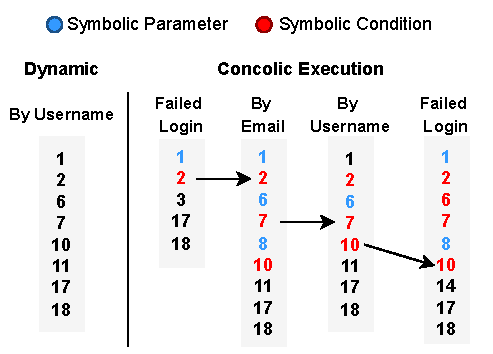
\includegraphics[width=0.5\linewidth]{figures/ad/code_sample_concolic.pdf}
	\caption{Dynamic code-coverage of a successful login attempt vs. symbolic execution of the same entry point. In this sample, user-provided parameters (e.g., \texttt{\$\_POST[\textquotesingle{}user\textquotesingle{}]}) and database operations (e.g., \texttt{get\_user\_by()}) are symbolic. Arrows mark the exploration of new feasible branches as determined by the symbolic engine.}
	\label{fig:concolic_coverage}
\end{figure}

\begin{figure*}[t]
    \centering
    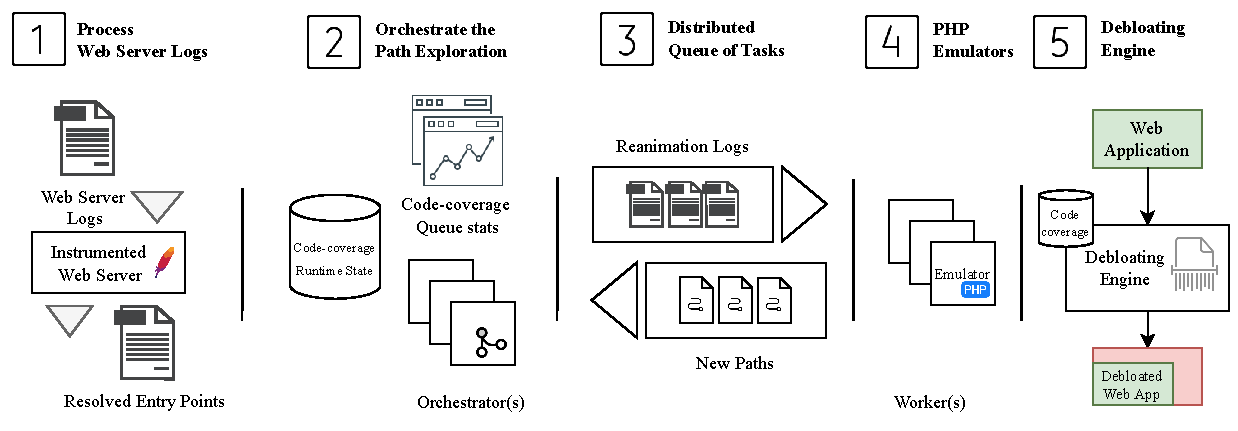
\includegraphics[width=\textwidth]{figures/ad/animatedead_diagram.pdf}
    \caption{Overview of Distributed \animatedead{}. In Stage 1, \animatedead{} analyzes the web server log files to generate unique web application entry points. Orchestrator nodes and workers (Stage 2 and 4) interact over message queues (Stage 3) to identify which paths should be explored by the emulators, \animatedead{} provides a realtime reporting panel that plots the size of the queue and newly identified code-coverage over time. Finally, in Stage 5, the overall code-coverage from concolic execution is incorporated for reachability analysis and unreachable modules from the entry points are debloated. Orchestrators and worker nodes run in container environments and can be scaled up on demand.}
    \label{fig:ad_diagram}
    \vspace{-1em}
\end{figure*}

\subsection{Application Entry Points}
The first step of our analysis consists of collection and processing of web application entry points.  
By using the existing logging mechanism of web servers, \animatedead{} is able to analyze web applications with \emph{no} extra runtime performance overhead. 
At the end of this stage (Step 1 in Figure~\ref{fig:ad_diagram}), we provide the list of PHP scripts and their concrete (e.g., GET parameters) and symbolic parameters (e.g., POST parameters, file uploads, cookies, etc.) to \animatedead{}'s PHP emulators for concolic execution. 

\subsubsection*{Analyzing Web Server Log Files} 
After collecting the web server logs for the target web application, \animatedead{} merges and de-duplicates the entries. 
The level of information provided for each entry point (i.e., concrete inputs) has a direct effect on the time of analysis. 
By shrinking the state space of the analysis via providing more detailed logs, we can reduce the total number of paths and reduce the overall analysis time. 

To that end, we experimented with the default fields of information in web server logs and extended logs. 
To generate extended logs, we use the web server's configuration options to include high level information such as the name (but not the value) of cookies, POST parameters and the file uploads. 
The extra information included in the extended logs limits the concolic execution to only explore paths that rely on the parameters that we have seen previously in the logs. 
Extended logs are particularly helpful for larger web applications such as WordPress and phpMyAdmin where a single entry point is responsible for a diverse list of features depending on the provided parameters. 
For instance, phpMyAdmin uses the same \emph{index.php} entry point combined with the \emph{target} GET parameter to generate the content of the requested pages. 
Providing this parameter to \animatedead{} allows it to only explore code-paths for the desired feature. 

\subsubsection*{Analyzing Log Files With URL Rewriting} 
PHP applications commonly incorporate URL rewriting to provide a user-friendly experience to their visitors and improve the search engine optimization of their website. 
Through this step, the original requested URIs are translated to one of the web application entry points either by the web server (e.g., Apache rewrite module and \texttt{.htaccess} files) or an internal module within the web application (i.e., custom routing modules). 
In the latter case, our PHP emulator resolves this mapping automatically without requiring any further action. 

For web applications using the web server's rewriting feature, the web server transforms the URIs before passing them to the web application. 
For such web applications, \animatedead{} dynamically replays the requests towards its integrated instrumented web server hosting a copy of target web applications and returns the translated entry points. 

\animatedead{} includes an instrumented Apache web server in its docker environment that hooks into every request and returns the translated URIs. 
By intercepting the incoming requests, \animatedead{} takes control of the execution and returns the resolved entry point after the web server applies the rewriting rules.
% Using PHP's \texttt{auto\_prepend\_file} directive, \animatedead{} takes control of the execution while the web server acts upon the original rewriting rules from the source code of target web applications under analysis. 
% This option can be enabled through \animatedead{}'s configuration file. 

\subsection{PHP Emulator}
Concolic execution requires a modified PHP execution environment that can operate based on symbolic parameters. 
We developed a PHP emulator for \animatedead{} that closely represents the PHP engine itself and operates based on the source code of PHP scripts. 
The analysis for each PHP application starts by parsing each entry point (e.g., \emph{index.php}) into it's respective Abstract Syntax Tree (AST) and traversing it. 
Through this traversal, certain PHP instructions will expand the AST during emulation. 
File inclusions, class instantiations, function calls and dynamic code generation routines (e.g., \texttt{eval}) can add new nodes to the AST. 

\animatedead{}'s emulator executes the PHP instructions of the program under analysis and resolves the dynamic code structures to generate a complete AST. 
In practice, resolution of dynamic code structures requires the precise implementation of every language construct and modeling its effects on the state of the emulator (i.e., active namespaces, current object pointers, variable scopes, function calls and return values, etc.). 

In \animatedead{}, beyond modeling the 188 standard PHP opcodes~\cite{popov}, we model the built-in PHP functions that affect the state of the emulator (e.g., loading new classes and defining new constants). 
For the majority of the self-contained PHP built-in functions that do not change the state of the emulator or manipulate the flow of execution such as \texttt{date}, \texttt{print}, \texttt{explode}, \texttt{file\_exists}, etc. we first resolve their arguments and then, invoke the original implementation in the PHP engine. 
For functions that rely on the state of the emulator (e.g., \texttt{class\_exists}, \texttt{define} (defines a new constant), \texttt{reflection APIs} (rely on autoloader and loaded classes and can invoke new code), \texttt{eval}, etc.), we provide our own implementation in the emulator. 
After a careful review of PHP documents and the list of built-in functions used in popular PHP applications, we identified 92 functions that required a custom implementation in our emulator. 

\animatedead{}'s PHP emulator is written in PHP 7.4 and is capable of emulating PHP 5.x and 7.x. 
The emulator imports all the environment variables and predefined constants (e.g., PHP version, default include path, etc.) from an existing web server environment. 
Moreover, analysts using \animatedead{} can override any desired API through the provided configuration file. 

We built our PHP emulator by extending the emulator developed by Naderi et al. called MalMax, which the authors combined with counterfactual execution to uncover the hidden behavior of obfuscated PHP malware~\cite{naderi2019malmax}. 
MalMax was originally built for PHP 5, and did not support symbolic execution. 
We spent over 13 person/months developing and testing our PHP emulator that supports the PHP language features used by popular PHP applications. 

One of our main contributions to MalMax's emulator is the distributed symbolic execution engine. 
Moreover, we added support for integral features of the PHP language to our emulator including the new PHP 7 instructions, object orientation features (e.g., inheritance, interfaces, etc.), closures, anonymous functions, namespaces, and reflection. 
Through this effort, we have doubled the code size of the original PHP emulator of MalMax, and the final \animatedead{} (i.e., emulator plus distributed execution environment) is more than five times the size of the initial emulator. 

\subsection{Handling Symbolic Operations and Logic}
\animatedead{} uses a configurable list of symbolic inputs (i.e., user-provided variables and system APIs). 
In this section, we explain the design details of our concolic emulator, including the type tracking, value set analysis, and the transition from symbolic to concrete values. 



\subsubsection{Concolic Execution}
\label{sec:concolic_translation}
One of the main requirements of a symbolic execution engine is to continue the program's execution with an abstract state of variables. 
At a high level, when dealing with symbolic program variables, PHP instructions such as conditionals would need to explore all the feasible branches when provided with a symbolic condition. 
Similarly, assignment instructions propagate the symbolic values upon their execution.

Our emulator incorporates type tracking to extract the type of symbolic variables even when the actual value is unknown. 
The variable type information is then used to skip the exploration of unsatisfiable branches. 
We model built-in functions that rely on variable types (e.g., \texttt{is\_int}) in the emulator for an accurate execution. 
Similarly, we include our own implementation for instructions that dynamically add new nodes to the AST (i.e., dynamic file inclusion, dynamic function calls, and dynamic object instantiation). 
More specifically, \animatedead{} uses the information available through the execution environment to transform the symbolic variables to their concolic equivalents. 
We will discuss this in more detail later in this section.

An example of this transition is reflected in file export format selection in phpMyAdmin which includes options such as SQL, CSV, Zip, etc. 
Given a symbolic export type in the form of user-controlled variable, \animatedead{} cannot statically determine which of the underlying export plugins should be loaded. 
The \texttt{Plugin\_loader} module within phpMyAdmin performs a series of string operations to sanitize the user input and to transform the selected export format to one of the available plugins on the file-system under the \texttt{libraries/plugins/export/} directory. 
As a result, by following the conditions enforced on the export format variable through execution (e.g., fixed prefix, file extension, and allow-list membership checks), \animatedead{}'s emulator can accurately identify the list of available export plugins in phpMyAdmin. 
Then, the emulator will explore the execution of the underlying entry point using each individual export plugin. 

\paragraph{Type tracking and value set analysis:} 
We have augmented our PHP emulator to track the type of symbolic variables based on known return type of PHP instructions and APIs. 
For instance, casting a symbolic variable to a specific type or invoking built-in functions with known return types (e.g., \texttt{substr} $\rightarrow$ \texttt{string}, or \texttt{isset} $\rightarrow$ \texttt{boolean}) will determine the resulting type of that variable. 
Unfortunately the information about the type of return values from PHP built-in functions is not available through the PHP reflection API. 
Instead, we extracted this information from the PHP documentation and incorporated it in \animatedead{}. 

Moreover, we model regex and string operations (e.g., \texttt{strncmp(\textquotesingle{}pma\textquotesingle{}, \$cookie\_name, 3) \!= 0}) as part of our emulator. 
By doing so, for path conditions that rely on these operations, we track the constraints applied to the underlying variables. 
This way, \animatedead{} can determine non-feasible conditions and refrain from exploring them. 

Lastly, we perform a scope-specific value set analysis. 
Web applications commonly perform allow-list and block-list checks to sanitize user-provided parameters and database sourced values. 
For instance, phpMyAdmin performs the following allow-list check to sanitize and validate the user-provided viewing mode in the reporting tabs: \texttt{in\_array(\$\_REQUEST[\textquotesingle{}viewing\_mode\textquotesingle{}], array(\textquotesingle{}server\textquotesingle{}, \textquotesingle{}db\textquotesingle{}, \textquotesingle{}table\textquotesingle{})}. 
When exploring paths that satisfy this symbolic condition, \animatedead{} limits the possible values of the symbolic \texttt{\textquotesingle{}viewing\_mode\textquotesingle{}} parameter to the values in the corresponding array (i.e., \texttt{\textquotesingle{}server\textquotesingle{}}, \texttt{\textquotesingle{}db\textquotesingle{}}, or \texttt{\textquotesingle{}table\textquotesingle{}}). 
This feature helps reduce the total number of explored branches and also aids the concolic engine when transitioning from symbolic values to their concrete counterparts. 


\paragraph{Transition from symbolic to concrete values:} 
The main benefit of symbolic execution is that each symbolic value represents all the possible values for that variable. 
As a result, it is beneficial to continue the execution with symbolic values. 
However, there exists scenarios in which \animatedead{} cannot continue executing the target application symbolically. 

Whenever our emulator reaches a PHP instruction that can change the structure of the AST by adding new files or calling new functions, \animatedead{} must replace the symbolic inputs of that API with its concrete counterparts. 
Examples of the APIs that add new nodes to the AST are file inclusion APIs (e.g., \texttt{include \$var}), class instantiations and static function calls that trigger the PHP autoloader (e.g., \texttt{new \$var} or \texttt{\$var::static\_function()}), reflection APIs, variable function calls (\texttt{\$var()}), APIs accepting a callback (e.g., \texttt{call\_user\_func(\$var)} and \texttt{preg\_replace\_callback(/regex/, \$var)}). 

In any of the aforementioned cases, \animatedead{} will rely on the information available from the execution environment to transition to concrete values. 
Most commonly, this step would consist of using the type information to determine the class type (for object instantiation), mapping the string operations to the file system or using the information from the value set analysis to determine the candidate values for each symbolic variable. 

Whenever the emulator faces more than one concrete option for a symbolic variable, it will create a new task including the code-coverage of the current execution and information about the concrete values for the target variable and add this task to the queue for future concolic execution (bottom queue in Step 3 in Figure~\ref{fig:ad_diagram}). 
Orchestrators process the code-coverage of each execution. 
Discovery of new code-coverage increases the priority of descendant paths of the current execution. 
\animatedead{} provides a configuration option to limit the total number of concrete values added from each point in the web application. 
% Based on our observations on PHP applications and their coding patterns, we set this limit to 20. 

In the scenario where symbolic execution cannot provide any information about the value of variables used in dynamic file inclusions or function calls, \animatedead{} would not be able to correctly determine the target files and functions to execute next. 
While in theory such code structures exist, and they could lead to false positives, in practice, we did not observe \emph{any} of them. 
An unbound symbolic file inclusion or function call may be rooted in non-sanitized user controlled variables or parameters coming from the database. 
In both scenarios, this could signal the presence of a first or second order injection style vulnerability and requires further attention. 
We incorporated safety checks within \animatedead{} to prevent the inclusion of an uncontrollably large number files or functions when the symbolic parameter is unbound and instead, we alert the analysts. 

\subsubsection{Emulation Replay} 

Throughout the analysis of PHP scripts, for every branch with symbolic condition, \animatedead{} explores all feasible paths. 
Similarly, when transitioning from symbolic to concrete values, multiple execution states are added to the queue. 
Upon facing more than one path to explore, the emulator produces a log called ``reanimation log'' which marks the currently explored branches and lists the next symbolic branch that should be explored. 
Using the reanimation logs, \animatedead{} instructs the emulator in worker nodes to replay the same execution and explore new branches within the code (top queue in Step 3 of Figure~\ref{fig:ad_diagram}). 


\subsubsection{Sources of Symbolic Information} 

In our analysis, we marked HTTP requests and their parameters, database APIs, and network APIs as symbolic. 
Therefore, the result of the analysis is a generalization over \emph{all} the possible values for the parameters present in the web server logs for the application under analysis. 
In our study we opted to run our analyses with an abstract application database. 
This way, our analysis generalizes for \emph{all} deployments of the web applications with any state of the database (i.e., successful and failed connections, empty and non-empty tables, etc.). 
Lastly, we mark network request responses as symbolic to account for successful and failed requests (e.g., checking for updates).

For HTTP requests, we instruct \animatedead{} that HTTP Cookies, Session variables, and File upload and POST parameters (For POST requests) are symbolic. 
This is based on the intuition that web servers will log HTTP GET request parameters and their values by default (i.e., URL query strings) but the value of cookies, session variables, and POST parameters are not included in neither default nor extended logs as they can include sensitive information. 
For database abstraction, we referred to the PHP language documents to extract the list of database APIs for popular database backends~\cite{phpdatabaseapis} and marked them as sources of symbolic information. 
Lastly, we marked PHP cURL APIs as symbolic to abstract the effect of network requests. 

\paragraph{Handling file uploads and file modifications/deletions:} 
PHP engine stores information about the uploaded files in the \texttt{\$\_FILES} super global variable. 
Each entry in this array corresponds to one of the user-uploaded files and contains information such as name, mime-type, temporary name (i.e., temporary file storage under /tmp/php/ directory by default), error (error code or 0 if successful), and size (upload size in bytes). 

For entry points with file uploads, \animatedead{} populates this super global variable with symbolic entries including successful and failed file uploads. 
Moreover, file operation APIs (e.g., \texttt{fopen, file\_get\_contents}, etc.) are modeled inside our emulator to handle symbolic file uploads. 
That is, opening a symbolic file will return a file with symbolic content. 
All web applications in our dataset perform file upload operations and our tests invoke the underlying entry points. 

When running multiple concolic execution workers in parallel, we isolate the changes they make to the file system to prevent side effects on other executions. 
\animatedead{} intercepts the APIs used to modify (e.g., \texttt{file\_put\_contents}) or remove files (e.g., \texttt{unlink}) and changes made through these APIs are only visible to the currently running execution. 
Therefore, file system modifications from one worker do not affect future executions and other workers. 

\subsection{Distributed Concolic Execution} 

Throughout the analysis of target applications, \animatedead{} will explore millions of different paths. 
To scale up the analysis, we designed a distributed environment with various worker processes running our PHP emulator. 
In this setup, we designate a group of orchestrator nodes responsible for the code-coverage analysis of the workers and prioritization of next paths to explore (Step 2 in Figure~\ref{fig:ad_diagram}). 
Orchestrators compare the code-coverage of current execution with the previously explored code and prioritize the analysis of unexplored branches, specifically the descendants of executions that resulted in the exploration of new parts of the code-base. 

\subsubsection{Path Prioritization}

We try to address the problem of state space explosion from two directions:
\begin{itemize}
    \item Eliminating unsatisfiable paths and limiting the total number of explored paths.
    \item Prioritizing paths based on their likelihood to explore unique parts of the codebase.
\end{itemize}

\paragraph{Reducing the total number of feasible paths:} 
Through close inspection of the structure of popular web applications, we identified that the majority of symbolic conditions check for presence or absence of user-provided parameters. 
These parameters usually dictate the main control flow of the entry points (e.g., providing username and password in a login request). 

Given the list of user controlled parameters (i.e., Post, Cookie, and Session variables) in phpMyAdmin, we analyzed the constraints for symbolic conditions. 
Overall, we identified that on average, 72\% of symbolic conditions only check for presence or absence of such parameters through the \texttt{isset} and \texttt{empty} built-in functions. 

Based on this observation, we decided to include the name (and not the value) of these parameters in the extended web server logs. 
This way, we will have the list of provided parameters by the users for POST requests and file uploads, thereby, significantly reducing the number of symbolic paths to be explored by \animatedead{}. 
% Moreover, we use the type tracking of \animatedead{} to eliminate the exploration of unsatisfiable branches in conditions on symbolic variables with a known type. 

\paragraph{Efficient path selection:} 
The exponential growth in the total number of paths in the application under analysis requires an effective path selection strategy. 
Symbolic execution engines employ problem-specific heuristics to analyze paths that are more likely to yield the desired results first. 
In the current setup, we opted to optimize paths to maximize code-coverage that is reachable from each entry point. 
\animatedead{} implements two path prioritization algorithms:

\begin{itemize}
    \item \textbf{DFS:} Using the depth-first-search algorithm, emulator worker processes will choose the last symbolic branch and flip its last symbolic condition to explore the new paths. This is the most straightforward approach that lacks any optimization for maximizing the explored code-coverage. 
    This method would result in the assignment of the same priority to all paths.
    \item \textbf{Branch-coverage guided prioritization:} In this setup, orchestrator nodes keep track of the branch coverage across all workers and prioritize paths that will explore the unseen branches. 
    For branches that have never been explored before, we set the priority to the maximum of 100. 
    After covering all the unique branches at least once, we calculate the priority by adding the total number of new lines discovered by each execution to 20\% of the priority of the parent branch for a maximum of 100. 
    This way, we focus on expanding the coverage in the vicinity of the recently discovered code, while gradually reducing the effect of the priority inherited from the parent execution to prevent the analysis from getting stuck in repetitive code structures. 
\end{itemize}

\begin{figure}[t]
    \centering
    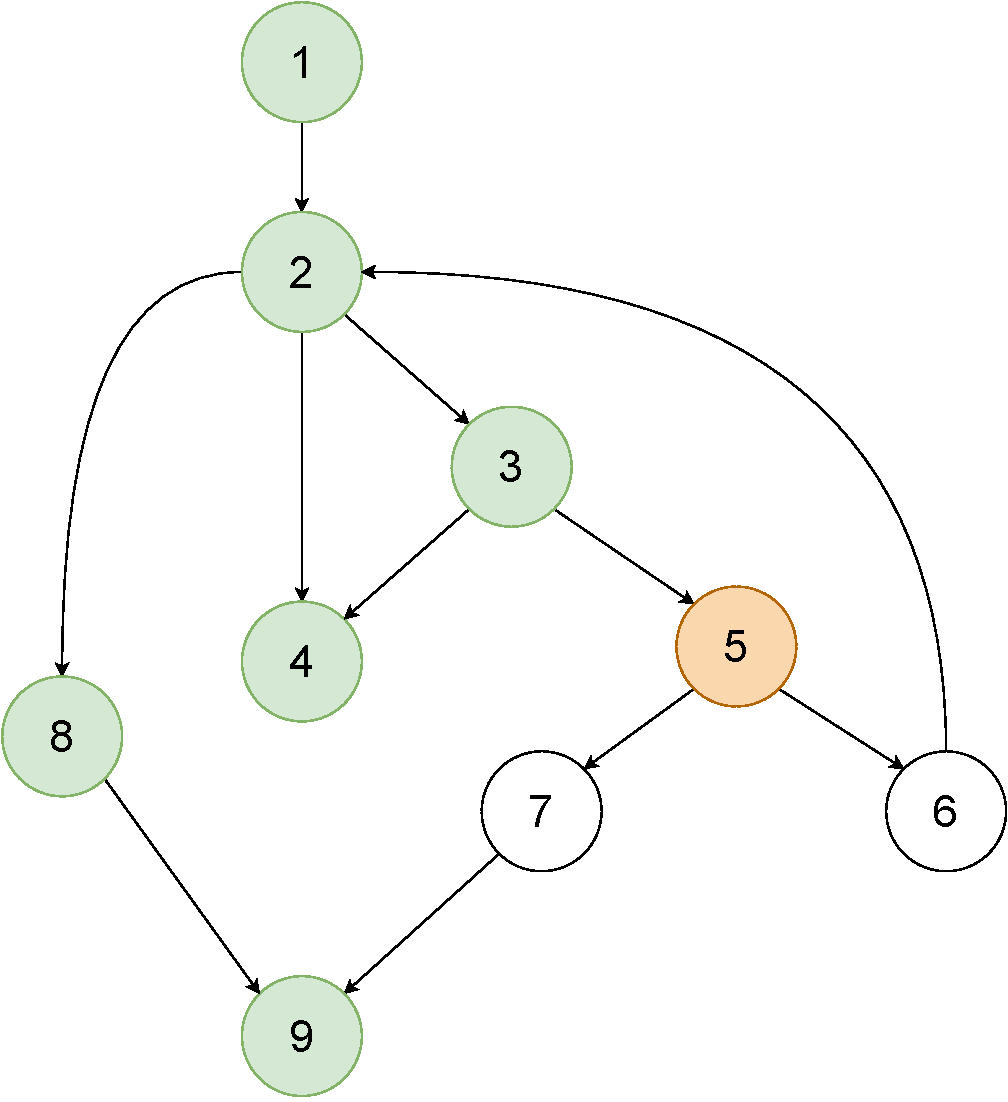
\includegraphics[width=0.3\linewidth]{figures/ad/AD_Path_Prio_CFG.pdf}
    \caption{Control flow graph example for path prioritization}
    \label{fig:cfg_pathprioritization}
\end{figure}

In the sample control flow graph in Figure~\ref{fig:cfg_pathprioritization}, assuming that all branches are symbolic, and the green nodes have been explored, once the two branches from node 3 are identified, the exploration of the branch towards node 5 receives the maximum priority of 100, as it has never been explored before. 
Moreover, immediate children of node 5 also inherit 20\% of the priority of their parent (i.e., 20) as they are the descendants of a newly discovered node. 

We store the reanimation logs on a priority queue, and as a result, workers will explore branches with a higher score first. 
We will compare and contrast the performance of DFS vs. Branch coverage path prioritization methods in Section~\ref{sec:path_priority}. 

\subsection{Debloating the Web Applications}
\animatedead{} produces the code-coverage information by merging the individual code-coverage from each execution of its workers. 
These results are analogous to the dynamic code-coverage used for debloating by the prior work. 
% The main benefit of this approach is the ability to perform an offline analysis based on web server logs.  
After generating the code-coverage for each web application, \animatedead{}'s debloating engine (Step 5 in Figure~\ref{fig:ad_diagram}) performs a reachability analysis and removes unused modules (i.e., files and functions) from the source code of web applications. 
We report the size reduction and security gains of debloating web applications via concolic execution and contrast the performance of this debloating scheme with the dynamic debloating of Less is More in Section~\ref{sec:results}. 

\subsection{Correctness Tests During Development}

During the initial stages of the development of our emulator, we started extracting the list of all PHP instructions from the PHP parser and provided an implementation of their logic in our emulator. 
Next, we analyzed the source code of popular PHP applications such as WordPress and phpMyAdmin to extract samples of interactions with symbolic variables (i.e., database queries, code handling HTTP requests, etc.).  

\paragraph{Unit Tests:} Based on the code snippets extracted from these applications, we created a total of 199 unit tests. 
We also included 19 unit tests provided by MalMax in our test suite~\cite{naderi2019malmax}. 

\paragraph{Functional Tests:} To complement the unit tests, we ran the Selenium scripts published as part of ``Less is More''~\cite{azad2019less} on debloated web applications. 
For the web applications in our dataset that are not part of LIM's dataset, we assembled a list of tasks exercising the main functionality of these web applications. 
For HotCRP, our scripts automate the setup of a conference and its deadline, user creation, submission of papers, and submitting reviews. 
For FluxBB, we automate user creation, posting new topics and changing user preferences. 
The extensive list of tasks that we automated with Selenium scripts is available in the Appendix. 

We then compared the list of invoked files and functions in response to requests towards debloated web applications and through iterative debugging we identified and addressed the implementation bugs that would prevent \animatedead{} from invoking the same modules as listed in the dynamic code-coverage traces. 
\section{Evaluation and Results}
\label{sec:results}

\begin{table}[]
    \caption{Number of automated daily requests towards web applications compared to the number of unique entry points.}
    \centering
    \begin{tabular}{|l|l|l|}
    \hline
    \textbf{Web Application} & \textbf{Requests/Day} & \textbf{Unique Endpoints} \\ \hline
    WordPress                & 558,576               & 152 (99.97\% $\blacktriangledown$)             \\ \hline
    phpMyAdmin               & 491,400               & 107 (99.98\% $\blacktriangledown$)             \\ \hline
    HotCRP                   & 175,848                 & 32 (99.98\% $\blacktriangledown$)              \\ \hline
    FluxBB                   & 63,624                & 17 (99.97\% $\blacktriangledown$)              \\ \hline
    \end{tabular}
    \label{tab:logreduction}
\end{table}

In this section, we employ \animatedead{} to debloat web applications. 
We start by collecting the list of entry points exercised while using popular web applications. 
We then configure \animatedead{} to explore feasible paths from those entry points. 
The result of this step is a list of exercised modules in target web applications. 
These modules are reachable from the list of entry points. 
Then, by removing the unused modules, we produce debloated web applications. 
In the remainder of this section, unless mentioned otherwise, we discuss the results of function debloating (i.e., removing functions with no callers) as it strictly outperforms file debloating.

Debloating based on concolic execution in \animatedead{} has multiple benefits over the previously explored dynamic debloating schemes that rely on runtime tracing to collect code-coverage information from users:

\begin{itemize}
    \item By relying on existing logging mechanism of web servers, we can collect usage traces for long periods of time for web applications with a large user base with small overhead.
    \item By analyzing each entry point in an abstract state (i.e., abstract request parameters, database, and network requests), the resulting code-coverage incorporates the functionality for all actions that are possible through each entry point and all possible database and network responses (i.e., including successful and failure cases), resulting in robust debloated applications (Section~\ref{sec:automated_random_testing}). 
\end{itemize}

\subsection{Experimental Setup}

In our evaluation, we focus on four popular web applications with different size and functionality. 
Our dataset includes phpMyAdmin 4.7 (database administration), WordPress 4.6.22 (content management system), HotCRP 3.0 (submission management), and FluxBB 1.5.11 (online forum platform). 

We run our analysis using 20 worker nodes (running \animatedead{}'s PHP emulator), and 5 orchestrators running inside Docker on an Ubuntu 22.04 LTS host with 20 CPU cores and 32GB of memory. 
For each web application, we follow their installation steps to generate the configuration files. 
This step is necessary as \emph{all} web applications in our dataset verify the presence of configuration files (e.g., \texttt{wp-config.php} for WordPress) and redirect user requests to the installation page if the post-installation files are absent from the file system. 

We configured concolic execution campaigns with the threshold of 24 hours, though in practice, the majority of entry points converge to their maximum code-coverage in less than one hour. 
Analysts can observe the progress made by \animatedead{} through the reporting panel and decide to terminate the analysis when \animatedead{} stops identifying new code-coverage or the queue becomes empty (i.e., all paths for an entry point are explored). 

\begin{figure*}[t]
    \centering
    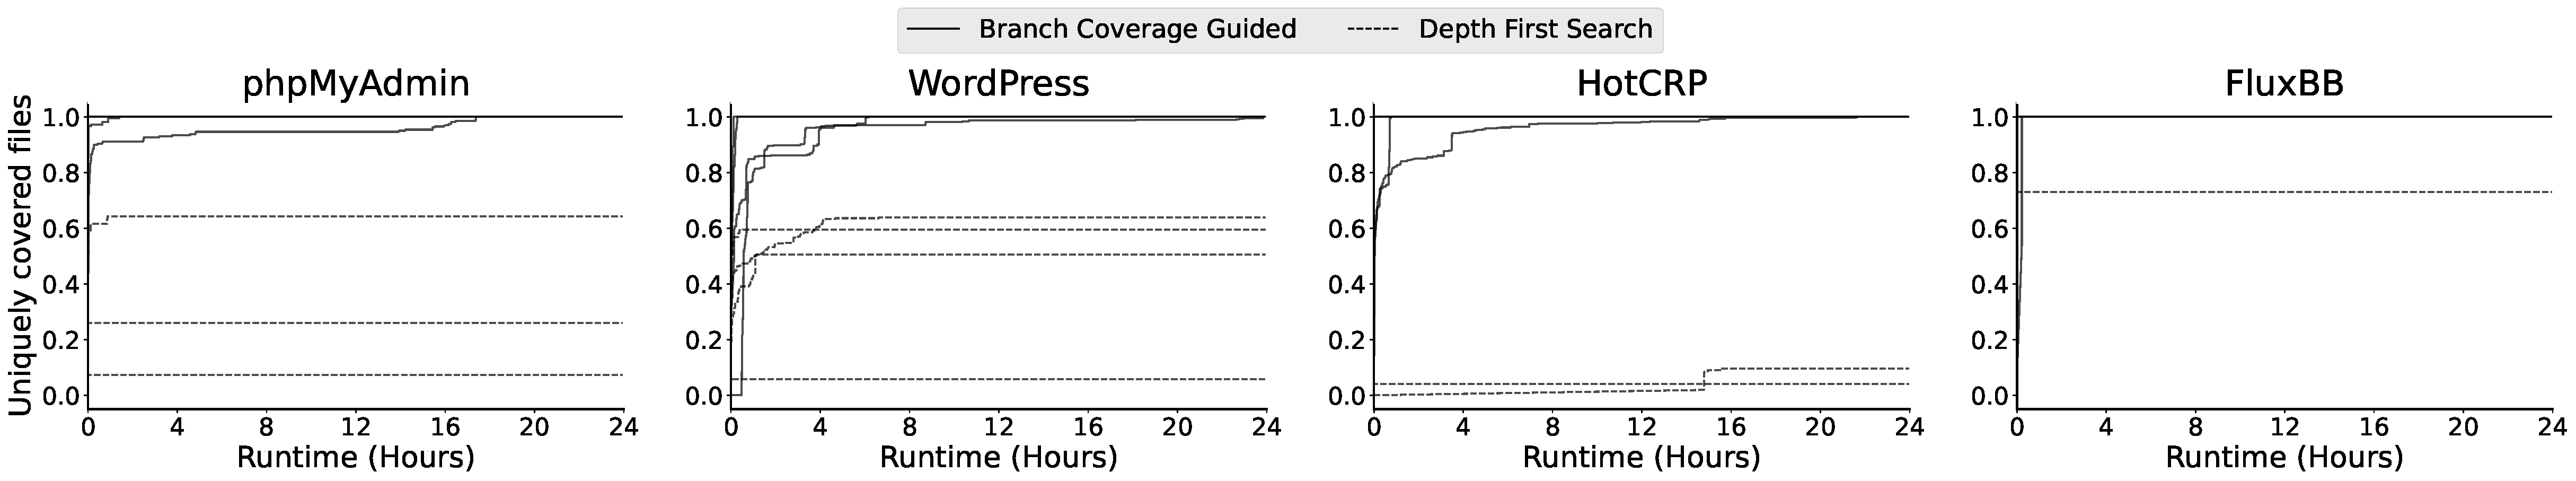
\includegraphics[width=\textwidth]{figures/ad/execution_convergence.pdf}
    \caption{Unique files discovered over time using DFS and Branch coverage guided path prioritization. Branch coverage approach results in a higher number of discovered files while DFS gets stuck in the same parts of the code.}
    \label{fig:execution_convergence}
\end{figure*}

\subsubsection*{Data Collection} 
To compare the debloating performance of \animatedead{} with prior work and to generate baseline code-coverage information for each entry point, we rely on the automated tests provided by the ``Less is More''~\cite{azad2019less}. 

We run the Selenium scripts from Less is More and the ones we built for HotCRP and FluxBB and collect the web server logs along with the dynamic code-coverage information from the Less is More framework. 
The code-coverage information for our web applications serves as the baseline code-coverage (i.e., dynamic code-coverage) for the remainder of our evaluation. 

We expect the resulting code-coverage of \animatedead{} to be a superset of the dynamic code-coverage information. 
Any file or function covered in the dynamic code-coverage that is missed by \animatedead{} would signify a false positive (i.e., removal of a feature that is required by users). 

\subsubsection*{Data Cleaning and Summarization} 
It is common for popular entry points (e.g., \texttt{index.php}) of web applications to receive a large number of requests. 
To prevent our tool from performing the same analysis multiple times unnecessarily, we only retain unique entry points and parameters from the web server logs. 

In the initial stages of the analysis, \animatedead{} removes duplicate log entries. 
Since we analyze the application with an abstract database, different values for the same parameters will have a similar effect (e.g., \texttt{?page\_id=1} or {\texttt{2}). 
This deduplication also shrinks the total number of entry points significantly. 
Table~\ref{tab:logreduction} lists the total number of log entry points produced over a 24 hour period by running the automated tests (Selenium, and crawler) repeatedly (simulating different users of a web application exercising the same functionality), compared to the final number of unique entries used by \animatedead{} for analysis. 
Across all web applications in our dataset, we observe a reduction of over 99.9\% in the number of unique entries to be analyzed. 
Moreover, web applications with a smaller code-base (i.e., FluxBB and HotCRP) produce fewer unique entry points. 

\subsection{Generating the Code-coverage}

We take the logs for each entry point in the web applications in our dataset and run them in \animatedead{} until either all paths are exhausted or a timeout of 24 hours is reached. 
\animatedead{} produces the code-coverage information for each execution in a separate log file. 
After merging the code-coverage of the explored paths from all entry points, we perform a module reachability analysis at the file and function level and debloat unreachable files and functions. 

\subsubsection{Efficient Path Selection}
\label{sec:path_priority}
Concolic execution generates an exponentially growing number of paths to be explored in target applications. 
This number grows based on the number of symbolic conditions in the target applications, for which \animatedead{} would need to explore the execution of all feasible branches. 
Concretely, \emph{N} consecutive symbolic branches would produce 2\textsuperscript{N} distinct paths. 

The prevalence of symbolic conditions and the total analysis time of each entry point directly affect the size of the queue which contains the future paths to be explored. 
Figure~\ref{fig:execution_convergence} depicts the unique files covered over time for a subset of entry points in each web application in our dataset during 24 hours of runtime. 

We ranked the time it takes for \animatedead{} to converge to the maximum file coverage for all application entry points. 
We then picked one entry point from each quantile for a total of four entries for each web application and path prioritization algorithm. 
For instance for WordPress, we plot ``admin-ajax'', ``customize'', ``index'', and ``login''  entry points sorted from most to least time to converge. 

Solid lines in Figure~\ref{fig:execution_convergence} represent the ratio of maximum covered files for each entry point when configuring \animatedead{} with Branch coverage guided path prioritization and dotted lines represent the runtime of the same entry points with DFS. 

For smaller applications such as FluxBB, the code-coverage converges in less than 10 minutes. 
For \emph{index.php} entry point of FluxBB, DFS fails to identify \emph{all} reachable files and is stuck in a repetitive code structure. 
For web applications with a modular architecture in which a larger number of PHP files are invoked to respond to each request, concolic execution requires a longer time to converge. 
This effect is visible for \emph{server\_import.php} entry point which explores code-paths for various export formats and takes 17 hours and 23 minutes to converge to its maximal code-coverage. 
Similarly, for WordPress, while the majority of entry points converge in the first few hours, certain entry points (e.g., such as \emph{admin-ajax.php} and \emph{customize.php}) take between 6 and 20 hours to converge. 

Across all web applications, we observe that branch coverage guided prioritization outperforms DFS in terms of the overall code-coverage. 
In practice, using the DFS algorithm leads to missing code-coverage (mainly due to investing the majority of execution time in the same subgraphs of the AST) which results in false positives after debloating. 

% \subsubsection{Correctness of Code-coverage}

% The validity of the debloated web applications by \animatedead{} relies upon the correctness of the resulting aggregate code-coverage for all application entry points. 
% There are two threats to the validity of this coverage:

% \begin{itemize}
%     \item Digression in the behavior of the PHP emulator compared to original PHP engine due to implementation flaws.
%     \item Feasible execution paths not being prioritized over previously explored paths, which results in missing code-coverage, due to suboptimal path prioritization.
% \end{itemize}

% After running the analysis of the entry points in \animatedead{} and collecting the overall code-coverage, we perform a reachability analysis and remove unused files and functions from the source code.
% This step provides us with the debloated web applications.

% In the absence of a ground truth dataset including all the reachable code from a given set of entry points for each web application, we rely on automated and random testing. 
% To empirically evaluate the correctness of \animatedead{} we devise two set of tests. 
% For each debloated web application, first, we replay the same tests used to collect the entry points and generate the dynamic code-coverage to make sure the debloated web applications did not lose any of their required functionality after debloating. 
% Second, we fuzz each entry point using an automated crawler. 
% In the case of correct debloating, the fuzzer would not trigger any debloated code while operating on the same entry points.

\subsection{Debloating Metrics}
We report the effectiveness of our debloating scheme through various source code and security metrics. 
These metrics are proxy variables to quantify the security improvements of debloated web applications. 

\subsubsection*{Logical Lines of Code (LLOC) Reduction} 
The reduction in the overall size of the code-base of an application has a direct correlation with the number of bugs present in it~\cite{mcconnell2004code}. 
Based on this intuition, shrinking the size of an application's code-base by removing unnecessary features reduces its attack surface and potential vulnerabilities. 
To measure this, we report the size of applications in our dataset before and after debloating in terms of logical lines of code (LLOC). 

\begin{table}[]
    \caption{LLOC reduction results of \animatedead{} compared to Less is More. Percentages represent the code reduction ratio.}
    \label{tab:lloc_reduction}
    \centering
    \begin{adjustbox}{max width=\columnwidth}
        \begin{tabular}{|l|l|l|l|}
        \hline
        \textbf{Web Application} & \textbf{Original} & \textbf{AnimateDead} & \textbf{LIM}  \\ \hline
        phpMyAdmin               & 112,220           & 35,162 (69\%)        & 26,094 (77\%) \\ \hline
        WordPress                & 73,201            & 39,529 (46\%)        & 36,738 (50\%) \\ \hline
        HotCRP                   & 40,898            & 30,814 (25\%)        & 24,407 (40\%) \\ \hline
        FluxBB                   & 6,683             & 3,550 (47\%)         & 3,141 (53\%)  \\ \hline
        \end{tabular}
    \end{adjustbox}
\end{table}

Table~\ref{tab:lloc_reduction} lists the size of web applications by \animatedead{} and Less is More (LIM). 
In this setup, \animatedead{} is performing concolic exploration of the same entry points as invoked by dynamic tests for LIM. 
As a result, the code-coverage produced by \animatedead{} is a superset of LIM. 
By looking at Table~\ref{tab:lloc_reduction}, we observe that for most web applications, debloating via concolic execution provides a size reduction comparable to the dynamic debloating. 

% Upon closer inspection of the files kept by \animatedead{} and removed by LIM, it is evident that dynamic debloating only kept the specific code path invoked via training while \animatedead{} kept the code responsible for the functionality that was reachable from each entry point including the error handlers and various code paths that lead to the invocation of the same feature. 

Upon closer inspection of the code that is only covered by \animatedead{} we identified features that were never exercised by Selenium tests but were reachable from the entry points. 
This enhances the usability of debloated web applications by \animatedead{} and reduces the likelihood of users invoking a removed function, which is a major drawback for dynamic debloating systems. 
For instance, we identified that the ``Forgot password'' functionality, reachable from the login entry point of WordPress was never invoked during the dynamic tests, and therefore, was removed by LIM. 
We verified that \animatedead{} keeps this functionality in WordPress, and as a result, allows users to use ``forgot password'' functionality even after debloating. 

\paragraph{Key point:} 
By incorporating concolic execution to explore the feasible program execution paths, \animatedead{} is able to generate the code-coverage of target web applications, reachable from their entry points. 
Using this code-coverage for reachability, allows us to produce debloated web applications that allow their users to perform all actions that are reachable from the previously invoked entry points, thus, reducing the likelihood of interacting with a debloated feature. 

\subsubsection*{Critical API Call Reduction}

\begin{figure}[t]
    \centering
    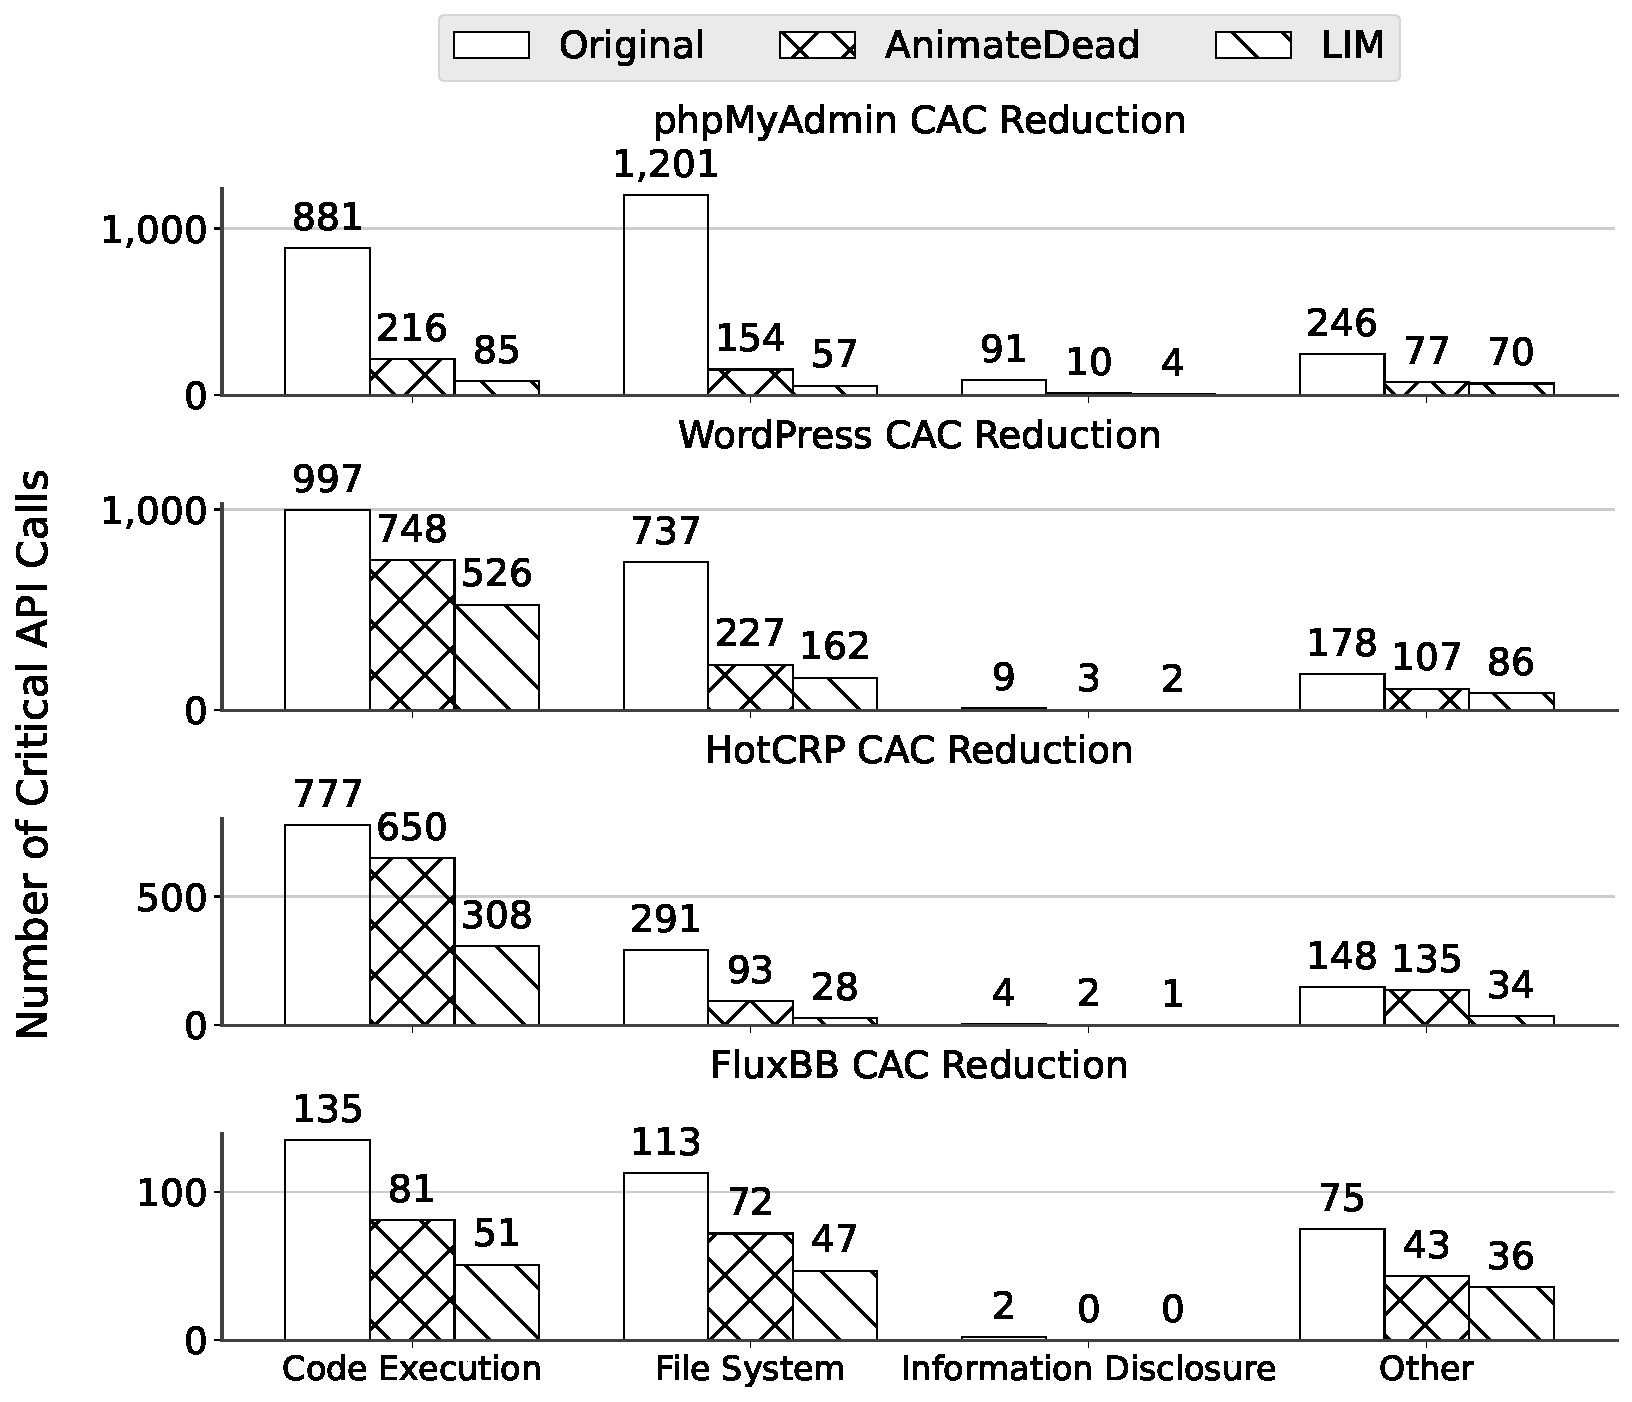
\includegraphics[width=0.9\columnwidth]{figures/ad/cac_reduction_bw.pdf}
    \caption{Reduction of Critical API Calls.}
    \label{fig:cac_reduction}
\end{figure}

The PHP engine interacts with its execution environment through a set of internal APIs. 
These APIs enable web applications to interact with the file system, network or even the database. 
Similar to system calls in binary applications, abuse of Critical PHP APIs (e.g., \texttt{eval}) is closely related to the amount of damage an attacker can do. 
Previous work in the area of exploit prevention and debloating has emphasized the importance of protecting critical APIs~\cite{Mishra2018, pappas2012kbouncer, fratric2012ropguard, bulekov2021saphire}. 

We use the list of 205 critical APIs used by RIPS to perform taint analysis on PHP applications for vulnerability discovery~\cite{dahse2010rips}. 
We report the removal of these APIs after debloating. 
For phpMyAdmin, we observe that \animatedead{} removes 75\% of code execution API calls, compared to 90\% reduction of Less is More. 
For other applications in our dataset, this reduction of critical API calls ranges from 10\% to 89\% for \animatedead{} and 50\% to 96\% for Less is More. 
As demonstrated in Figure~\ref{fig:cac_reduction}, debloating based on concolic execution of entry points results in a considerable reduction in critical API calls compared to the original applications, across all categories of critical APIs. 

\subsubsection*{CVE Reduction}
Orthogonal to size reduction, we measure the performance of debloating in removing historic vulnerabilities in the source code of an application. 
To that end, for web applications present on public CVE databases (phpMyAdmin and WordPress), we reuse the CVE to source code mapping information available in the prior work~\cite{azad2019less}.

Table~\ref{tab:cve_reduction} lists the removal of CVEs after debloating. 
For both web applications, file debloating of \animatedead{} and LIM remove the same number of CVEs. 
Similarly, for WordPress, function debloating of \animatedead{} and LIM retain seven CVEs. 
For phpMyAdmin, function debloating results show that \animatedead{}'s debloating retains three CVEs more than LIM. 

We analyzed the three extra CVEs. 
For the first vulnerability (CVE-2016-5703), LIM retains multiple call sites for the vulnerable function, none of which were invoked during the dynamic tests. 
Since the path conditions for these call sites rely on database values (i.e., symbolic), \animatedead{} correctly retains the vulnerable function to preserve the correct functionality. 
Second vulnerability (CVE-2016-6633) resides in the ``import'' page of phpMyAdmin. 
Selenium tests only import SQL files while phpMyAdmin supports seven formats (e.g., zip, CSV, XML). 
Since the uploaded file format is selected by the user and is therefore symbolic, \animatedead{} retains other import formats including the one with the vulnerability. 
Lastly, we analyzed CVE-2016-6619 which resides in ``recent favorite tables'' feature, if the users request the list of recent tables without having selected any tables before, the vulnerable function would be invoked. 

The performance of \animatedead{} and LIM in the removal of CVEs for WordPress is identical. 
For the three CVEs that were removed only by LIM, we analyzed the source code of phpMyAdmin and identified that in all cases, there exists at least one symbolic code path (based on user-controlled parameters or database values) that can call the vulnerable functions, and therefore, \animatedead{} correctly retained the CVEs to preserve the correct functionality in the debloated web application. 


\subsubsection*{Removal of Object Injection Gadgets}
Improper use of deserialization APIs in PHP can lead to object injection vulnerabilities. 
This vulnerability allows attackers to build a chain of function calls through existing classes in the vulnerable web applications--known as gadget chains--to mount exploits such as SQL injection, arbitrary file write, and even remote code execution. 

Removal of gadget chains via debloating protects web applications and complicates the exploitation of object injection vulnerabilities. 
We use PHPGGC, a public repository that tracks the known gadget chains in popular web applications and third-party packages~\cite{PHPGGC}, to identify gadgets for phpMyAdmin and its third-party packages as well as WordPress. 
Their dataset does not include gadgets for HotCRP and FluxBB and therefore we only report the gadget chain reduction for phpMyAdmin and WordPress.

We identified three gadget chains for phpMyAdmin and two for WordPress.
For WordPress, both \animatedead{} and LIM successfully removed all gadget chains protecting the web application against exploits even in the presence of an object injection vulnerability. 
In the case of phpMyAdmin, one out of the three gadget chains remains in the source code after debloating via both \animatedead{} and LIM. 
This gadget belongs to the tcpdf library used by phpMyAdmin to generate PDF files. 
The gadget chain makes use of the class constructor in the main module of tcpdf (i.e., \texttt{tcpdf.php}). 
phpMyAdmin invokes the constructor of all available Export modules (including the PDF format) upon using the database export functionality and as a result, this gadget chain--correctly--remains in the debloated web applications.

\begin{table}[]
    \caption{Reduction of CVEs for phpMyAdmin and WordPress with concolic debloating of \animatedead{} and dynamic debloating of Less is More. \animatedead{} and LIM columns show the number of CVEs remaining after debloating with the specified strategy (i.e., File vs. Function debloating).}
    \label{tab:cve_reduction}
    \centering
    \begin{adjustbox}{max width=\columnwidth}
    \begin{tabular}{|l|c|cc|cc|}
    \hline
    \multirow{2}{*}{\textbf{Web Application}} & \multirow{2}{*}{\textbf{Original}} & \multicolumn{2}{c|}{\textbf{AnimateDead}}                 & \multicolumn{2}{c|}{\textbf{LIM}}    \\ \cline{3-6} 
                                              &                                    & \multicolumn{1}{c|}{File} & \multicolumn{1}{c|}{Function} & \multicolumn{1}{c|}{File} & Function \\ \hline
    phpMyAdmin                                & 20                                 & \multicolumn{1}{c|}{12}    & 7                             & \multicolumn{1}{c|}{12}    & 4        \\ \hline
    WordPress                                 & 20                                 & \multicolumn{1}{c|}{19}   & 13                             & \multicolumn{1}{c|}{19}   & 13        \\ \hline
    \end{tabular}
    \end{adjustbox}
\end{table}

\subsection{Assessment of Correctness}
In this section, we discuss the experiments that we designed to evaluate the correctness of the debloated web applications by \animatedead{}. 
We envision several categorical threats to the correctness of debloated web applications (i.e., removal of required features): 

\noindent \textbf{Implementation bugs:} 
Any flaw in the implementation of the emulator which leads to a different outcome during the execution (e.g., taking a different branch) can potentially lead to missing code-coverage. 
To address this concern, first, we created unit tests to check for the core functionality of our emulator. 
Next, we extracted code structures that handled symbolic variables from popular PHP applications in our dataset and isolated the expected behavior to verify the correct emulation results in \animatedead{}. 
Lastly, we replayed the dynamic execution traces (i.e., Selenium tests) against debloated web applications to ensure that \animatedead{}'s debloating did not break any of the previously exercised functionality.

\noindent \textbf{State space explosion:} 
Another source of missing code-coverage is rooted in the state space explosion problem. 
For larger PHP applications in our dataset (i.e., phpMyAdmin, WordPress, and HotCRP), the total number of satisfiable symbolic conditions in the applications leads to the generation of an exponentially growing number of paths for each entry point. 

As a result, exploring every single path is not feasible, nor desired particularly because the majority of explored paths do not lead to the discovery of new files and functions.  
To address this challenge, as discussed in Section~\ref{sec:path_priority}, we proposed an efficient path prioritization strategy that in practice, addressed the path explosion issue in the context of producing the correct code-coverage for applications in our dataset. 

One of the key challenges of verifying the correctness of a debloating scheme is the lack of ground truth code-coverage information. 
Dynamic code-coverage traces can be used as a lower-bound of line-coverage. 
In the absence of an oracle that determines all the reachable lines of code from each entry point given a symbolic environment we rely on automated random testing. 

\subsubsection{Automated Random testing}
\label{sec:automated_random_testing}
We use ZAP Proxy~\cite{zapproxy} and its automated crawler to interact with the same entry points used for debloating. 
By performing random testing on the same entry points used for debloating, we automatically exercise the features that are reachable from the same entry points, which should be retained by \animatedead{}. 

We execute ZAP Proxy in spider and scan mode for up to 1 hour with the authenticated session cookies and login credentials of the web applications. 
Overall, ZAP sent 86,649 requests towards the four debloated web applications in our dataset. 
We instrumented these applications to log requests towards debloating files and functions and store the entry point for those requests. 
``Errors'' column  in Table~\ref{tab:dynamic_tests} indicates the total number of unique entry points that invoked a debloated module. 
Errors are considered false positives \emph{only if} they were triggered from one of the entry points that \animatedead{} used for debloating. 
The number of reported false positives in Table~\ref{tab:dynamic_tests} refer to the number of missing files or functions and not the number of entry points. 
After a close inspection, we attribute \emph{all} the errors for \animatedead{} debloated web applications to interaction of ZAP with new entry points. 
Conversely, for web applications debloated with LIM, we identified six missing functions in phpMyAdmin related to authentication cookies, error handling, and logging. 
Similarly for WordPress, six functions from themes, cookie and session management, and failed login module were removed that triggered an error by our crawler. 
Lastly, for FluxBB, we identified two missing functions from the database adapter and password verification modules. 

The results of dynamic tests indicate that given the same entry points, dynamic debloating schemes such as LIM rely on an extensive training stage to retain all the functionality that their users need. 
In contrast, concolic execution in \animatedead{} performs its analysis based on abstract inputs (e.g., correct and incorrect login credentials) and as a result, provides more robust debloated applications without relying on server side instrumentation and extensive training data. 

\begin{table}[]
    \caption{Automated random testing results including the total number of requests made by ZAP Proxy crawler, number of entry points that triggered an error and number of missing files or functions that triggered false positives (i.e., requests towards entry points from the logs that invoked a debloated module)}
    \label{tab:dynamic_tests}
    \centering
    \begin{adjustbox}{max width=\columnwidth}
    \begin{tabular}{|l|c|c|cc|}
        \hline
        \multirow{2}{*}{\textbf{Web Application}} & \multirow{2}{*}{\textbf{Requests}} & \multirow{2}{*}{\textbf{Errors}} & \multicolumn{2}{c|}{\textbf{False Positives}}               \\ \cline{4-5} 
                                                  &                                    &                                  & \multicolumn{1}{l|}{AnimateDead} & \multicolumn{1}{l|}{LIM} \\ \hline
        phpMyAdmin                                & 21,040                             & 6                                & \multicolumn{1}{c|}{0}           & 6                        \\ \hline
        WordPress                                 & 31,055                             & 102                              & \multicolumn{1}{c|}{0}           & 6                        \\ \hline
        HotCRP                                    & 16,021                             & 12                               & \multicolumn{1}{c|}{0}           & 0                        \\ \hline
        FluxBB                                    & 18,533                             & 3                                & \multicolumn{1}{c|}{0}           & 2                        \\ \hline
        \end{tabular}
    \end{adjustbox}
\end{table}
\section{Discussion}
In this section, we discuss some design decisions when building \animatedead{}. 

\paragraph{Path condition analysis:} 
Concolic execution engines often incorporate SMT solvers such as Z3~\cite{moura2008z3} to evaluate the feasibility of symbolic branches based on path constraints and replace symbolic variables with concrete samples. 
In this work, to reduce the complexity of our operations and reduce the overhead of SMT solvers, we opted to implement our context-specific concolic translator. 
As discussed in Section~\ref{sec:concolic_translation}, \animatedead{} tracks path constraints for strings, set operations (i.e., array membership checks and value set analysis), and variable types. 
Using this information, the emulator skips non-feasible branches and replaces symbolic variables with concrete values only when required (i.e., instructions that introduce new code to the AST). 

\paragraph{Runtime threshold and termination condition:} 
The decision to terminate a concolic execution campaign can determine the completeness of its results. 
Premature termination can lead to missed code-coverage and in turn, false positives in debloating. 
The two mainstream approaches to this problem are time-based thresholds (e.g., terminate the analysis after \emph{N} hours of no new discovery) or missing mass estimators~\cite{goodestimator}. 
The premise of an estimator is to determine, given the prior inputs and their unique code-coverage, what is the probability of the next input to explore new code-coverage. 

In this work, we opted to use a threshold of 24 hours based on our experiments. 
In practice, only a subset of all entry points in larger web applications require runtime of more than 1 hour. 
\animatedead{} provides a reporting panel that plots the new code-coverage information for each running campaign. 
We suggest that analysts oversee the convergence of new code-coverage discovery and terminate the analysis of each entry point after concolic execution stops identifying new code-coverage for an extended period of time. 

\paragraph{Single Page Applications (SPA):} 
These web applications incorporate JavaScript libraries and asynchronous requests to interact with the web server and navigate through the web application seamlessly. 
\animatedead{} operates based on web server logs, as a result, the client side intricacies of SPAs do not affect its analysis. 

% \paragraph{Concolic execution of other languages:} 
% We built \animatedead{} based on the PHP language, which is the most popular web development language used by more than 77.4\% of all websites~\cite{w3techphp}. 
% Majority of the development effort of this project is targeted towards the PHP language. 
% As a result, for \animatedead{} to support other languages, one needs to develop new concolic execution engines. 
% That said, given the similarity of web programming languages (e.g., dynamic constructs, use of callbacks, etc.), we envision that they can benefit from the design concepts of \animatedead{}. 

% \section{Related Work}

\paragraph{Symbolic and concolic testing} are powerful tools that fill the gap between static and dynamic analysis. 
Researchers have designed numerous binary testing and vulnerability discovery tools based on symbolic testing~\cite{cadar2008exe, cadar2008klee, chipounov2009selective, godefroid2012sage, cha2012unleashing, wang2017angr}. 
Running symbolic testing at the scale of large applications is challenging. 
This is mainly due to the rapid increase in the total number of paths to be explored, also known as state space explosion, as well as the overhead from the SMT solvers. 

One helpful technique used in symbolic web application analysis tools is to isolate the code for their target module before performing the symbolic analysis. 
For instance, Huang et al. built a file upload vulnerability discovery tool named UChecker~\cite{Huang2019}. 
In their tool, they perform an initial phase of static analysis to identify potentially vulnerable sinks. 
Then, through backward slicing, they isolate the code responsible for file upload functionality from user controlled sources to sensitive sinks. 
Similarly, Jensen et al. aid their static analysis by resolving dynamic file inclusions via dynamic analysis by incorporating web crawlers~\cite{jensen2012thaps}. 
They then perform static analysis to identify XSS vulnerabilities and finally validate their findings using symbolic execution. 
In both papers, the authors use symbolic execution to verify the reachability of the vulnerable sinks. 

% Godefroid et al. developed SAGE, a symbolic execution engine that targets security vulnerabilities in x86 binaries~\cite{godefroid2012sage}. 
% DART is another tool that uses the idea of symbolic execution to generate failure inducing test cases with concrete inputs to detect crashes and assertion violations in C programs~\cite{godefroid2005dart}. 

To combat the state space explosion problem, researchers have introduced various path prioritization algorithms. 
The simplest form of path exploration is breadth-first-search and depth-first-search, used by DART~\cite{godefroid2005dart}. 
Next to that, other heuristics such as ``reducing the number of redundant path explorations'', ``maximizing code-coverage'', and ``guiding the execution towards security sensitive APIs'' are implemented by researchers in tools such as KLEE~\cite{cadar2008klee}, EXE~\cite{cadar2008exe}, Mayhem~\cite{cha2012unleashing}, S2E~\cite{cha2012unleashing}, and AEG~\cite{avgerinos2014automatic}. 

In \animatedead{}, we designed our path prioritization heuristic to optimize for maximum code-coverage, inline with our goal to use the code-coverage for software debloating. 
We extended the PHP emulator from MalMax developed by Naderi et al.~\cite{naderi2019malmax,naderi2019cubismo}. 
In their work, the authors build a PHP emulator capable of counterfactual execution to uncover the original intents of obfuscated PHP malware. 
While PHP malware uses specific APIs to remain hidden and perform its malicious actions, complex PHP applications interact with a large number of PHP APIs. 
To be able to perform an end-to-end analysis of these applications, we extended MalMax by adding support for symbolic execution, and implementing the features used in popular PHP applications. 

\paragraph{Software debloating} 
Researchers have approached the idea of debloating from various aspects ranging from the kernel~\cite{abubakar2021shard}, container environments~\cite{rastogi2017cimplifier, 259711} to binaries~\cite{hasan2022decap, redini2019b, heo2018effective, ghavamnia2020temporal, mishra2020saffire, koo2019configuration, quach2018debloating}, web browsers~\cite{snyder2017most, qian2020slimium}, and web applications~\cite{azad2019less, bulekov2021saphire, mininode, jahanshahi2020you}.

In this paper, we use the ``Less is More'' framework of Amin Azad et al.~\cite{azad2019less} to generate a baseline code-coverage to assess the results of \animatedead{} and generate our entry points based on the Selenium tests developed as part of LIM. 
While the goal of \animatedead{} debloating is not to outperform LIM, we demonstrate that despite the generalizations made by concolic execution, our debloating statistics and security improvements are on par with the dynamic debloating of LIM. 

Unlike LIM, \animatedead{} does not rely on an extensive training phase and can perform its analysis offline with virtually \emph{zero} overhead on production execution environments. 

Web applications debloated by \animatedead{} can benefit from the protections offered by other orthogonal attack-surface reduction and API specialization schemes such as Saphire~\cite{bulekov2021saphire} and SQLBLock~\cite{jahanshahi2020you} to protect against SQL injection vulnerabilities in the remaining SQL API calls required by users and to confine the web application based on a generated profile of system-calls to limit the potential damage from code execution exploits.


% \section{Availability}

To ensure transparency while promoting future work in the space of PHP concolic execution and debloating web applications, we will provide public access to \emph{all} developed code and artifacts upon publication of this paper. 
\section{Summary}
In this paper, we introduced \animatedead{}, a PHP emulator capable of analyzing web applications with abstract inputs. 
We presented the design details of its concolic execution engine and reviewed our approach to building a distributed analysis framework. 

Recognizing the practical limitation of dynamic debloating systems, namely their need for extensive training data and their high runtime overhead, 
we incorporated \animatedead{} together with the readily available web server logs to perform a reachability analysis from each entry point in the web applications in the form of code-coverage information. 
Using this information, we performed an offline analysis in the form of concolic execution and a module reachability analysis to remove unreachable modules. 
We debloated four popular PHP applications and demonstrated the security improvements of our method to be comparable to dynamic debloating schemes. 
\animatedead{} is capable of producing debloated web applications that are 47\% smaller and include 55\% fewer critical API calls. 

Finally, we show that the concolic analysis of entry points by \animatedead{} leads to debloated web applications that generalize over \emph{all} inputs to the same entry points where dynamic debloating schemes would have a breakage.  
Overall, our results demonstrate that concolic execution is a practical method for debloating web applications that addresses core limitations of prior work.

\chapter{Conclusion}
\label{chap:conclusion}

In this dissertation we evaluated the benefits of software debloating in terms of improving the security of web applications. 
To that end, we presented ``Less is More'', our dynamic debloating pipeline that simulates usage behaviors and uses dynamic analysis to debloat web applications with file and function level granularity. 
Moreover, we introduced multiple metrics to quantify the security benefits of debloating web applications. 
By evaluating our framework on four popular PHP applications (phpMyAdmin, MediaWiki, Magento, and WordPress) we demonstrated a reduction of 46.8\% on average in LLOC (Logical Lines Of Code) and a comparable reduction in the cyclomatic complexity of debloated applications. 
We discussed how the structure of applications affects the debloating results (e.g., the monolithic design of WordPress leads to less debloating compared to modular web applications such as Magento). 
From the perspective of code-reuse attacks, we witnessed that debloating disrupts the majority of publicly known gadget chains used in object injection attacks. 
Similarly, debloating removed up to 60\% of high impact CVEs. 

After demonstrating the effectiveness of debloating web applications from a security perspective, we proposed a novel approach for debloating. 
Unlike prior work which focus on producing a single debloated application, we explored the idea of ``role-based debloating''. 
Our system named \dbltr{} considers the code-coverage information of individual web-application users and clusters the users with similar usage behavior together. 
Based on these clusters, \dbltr{} produces multiple versions of debloated web applications, each tailored to a specific group of users. 

We initiated this project by conducting a user study to understand how experienced administrators and developers interact with web applications. 
Motivated by our initial findings, we incorporated the code-coverage traces from the user study in \dbltr{} to produce debloated web applications and evaluate their security-related metrics. 
Our results show that role-based debloating can further reduce the size of web applications in terms of LLOC by 30\%, and remove severe security vulnerabilities by up to 80\% for some roles, compared to the globally debloated application similar to our approach in Chapter~\ref{chap:lim}. 
\dbltr{} also incorporates content-delivery modules to transparently extract user identities from login requests and route their requests towards their custom debloated web applications. 
Overall, our results indicate that role-based debloating is a practical approach with tangible security benefits. 

Lastly, to address the drawbacks of dynamic debloating schemes, we designed our concolic execution engine named \animatedead{}. 
Using this system, we performed a module-reachability analysis from the entry points of web applications and removed unused code based on the exercised entry points. 
We showed that concolic execution can provide comparable security gains in debloated web applications on par with dynamic schemes. 
Specifically, we demonstrated a reduction of 47\% in LLOC and 55\% reduction in critical API calls for web applications debloated by \animatedead{}. 

Through the analysis of modern web applications and the development of debloating frameworks, we supported our thesis statement that modern web applications expose an unnecessarily large attack surface due to code-bloat. 
We proposed dynamic and hybrid debloating mechanisms that can successfully identify unused modules in web applications and automatically debloat them, thereby, protecting web applications and their users against the exploitation of vulnerabilities. 
%%%%%%%%%%%%%%%%%%%%%%%%%%%%%%%%%%%%%%%%%%%%%%%%%%%%%%%%%%%%%%%%%%%%%%%%%%%%%%%%
\bibliographystyle{unsrtnat}
\renewcommand{\baselinestretch}{1}
\normalsize

\clearpage
\newpage
\phantomsection%
\addcontentsline{toc}{chapter}{\numberline{}{Bibliography}}%
\bibliography{ref}

\clearpage
\newpage

\appendix
\section*{Appendix}

\begin{table}[ht!]
  \footnotesize
  \centering
\caption{Comprehensive list of tutorials collected from the first two pages of Google search results}
\label{table:listoftutorials}
\scalebox{0.7}{
\begin{tabular}{|l|p{20cm}|}
\hline
\multicolumn{2}{|c|}{\textbf{phpMyAdmin}}  \\ \hline
  \href{https://web.archive.org/web/20181112232555/https://www.siteground.com/tutorials/phpmyadmin/}{A}                                                             & \href{https://www.siteground.com/tutorials/phpmyadmin/}{https://www.siteground.com/tutorials/phpmyadmin/}                                    \\ \hline
  \href{https://web.archive.org/web/20181112233149/https://www.reg.ca/faq/PhpMyAdminTutorial.html}{A}                                                               & \href{https://www.reg.ca/faq/PhpMyAdminTutorial.html}{https://www.reg.ca/faq/PhpMyAdminTutorial.html} \\ \hline
  \href{https://web.archive.org/web/20181114201249/https://www.w3resource.com/mysql/administration-tools/phpmyadmin-tutorial.php}{A}                                & \href{https://www.w3resource.com/mysql/administration-tools/phpmyadmin-tutorial.php}{https://www.w3resource.com/mysql/administration-tools/phpmyadmin-tutorial.php} \\ \hline
  \href{https://web.archive.org/web/20181112233311/https://code.tutsplus.com/tutorials/installing-and-using-phpmyadmin-for-web-development--cms-21947}{A}           & \href{https://code.tutsplus.com/tutorials/installing-and-using-phpmyadmin-for-web-development--cms-21947}{https://code.tutsplus.com/tutorials/installing-and-using-phpmyadmin-for-web-development--cms-21947} \\ \hline
  \href{https://web.archive.org/web/20181112233410/https://www.homeandlearn.co.uk/php/php12p2.html}{A}                                                              & \href{https://www.homeandlearn.co.uk/php/php12p2.html}{https://www.homeandlearn.co.uk/php/php12p2.html} \\ \hline
  \href{https://web.archive.org/web/20181112233639/https://www.wpbeginner.com/beginners-guide/beginners-guide-to-wordpress-database-management-with-phpmyadmin/}{A} & \href{https://www.wpbeginner.com/beginners-guide/beginners-guide-to-wordpress-database-management-with-phpmyadmin/}{https://www.wpbeginner.com/beginners-guide/beginners-guide-to-wordpress-database-management-with-phpmyadmin/} \\ \hline
  \href{https://web.archive.org/web/20181112233730/http://members.ipage.com/knowledgebase/read_article.bml?kbid=5923}{A}                                            & \href{http://members.ipage.com/knowledgebase/read_article.bml?kbid=5923}{http://members.ipage.com/knowledgebase/read\_article.bml?kbid=5923} \\ \hline
  \href{https://web.archive.org/web/20181112233831/https://www.digitalocean.com/community/tutorials/how-to-install-and-secure-phpmyadmin-on-ubuntu-16-04}{A}        & \href{https://www.digitalocean.com/community/tutorials/how-to-install-and-secure-phpmyadmin-on-ubuntu-16-04}{https://www.digitalocean.com/community/tutorials/how-to-install-and-secure-phpmyadmin-on-ubuntu-16-04} \\ \hline
  \href{https://web.archive.org/web/20181112233904/https://www.fastwebhost.com/tutorials/knowledge-base/phpmyadmin-tutorial-administration-2/}{A}                   & \href{https://www.fastwebhost.com/tutorials/knowledge-base/phpmyadmin-tutorial-administration-2/}{https://www.fastwebhost.com/tutorials/knowledge-base/phpmyadmin-tutorial-administration-2/} \\ \hline
  \href{https://web.archive.org/web/20181112234156/https://www.tutorialspoint.com/cpanel/cpanel_phpmyadmin.htm}{A}                                                  & \href{https://www.tutorialspoint.com/cpanel/cpanel_phpmyadmin.htm}{https://www.tutorialspoint.com/cpanel/cpanel\_phpmyadmin.htm} \\ \hline
  \href{https://web.archive.org/web/20181112234218/https://www.w3schools.com/php/php_mysql_intro.asp}{A}                                                            & \href{https://www.w3schools.com/php/php_mysql_intro.asp}{https://www.w3schools.com/php/php\_mysql\_intro.asp} \\ \hline
  \href{https://web.archive.org/web/20181112234543/https://pimylifeup.com/raspberry-pi-mysql-phpmyadmin/}{A}                                                        & \href{https://pimylifeup.com/raspberry-pi-mysql-phpmyadmin/}{https://pimylifeup.com/raspberry-pi-mysql-phpmyadmin/} \\ \hline
  \href{https://web.archive.org/web/20181112234617/https://www.webhostface.com/kb/knowledgebase/mysql-search-replace/}{A}                                           & \href{https://www.webhostface.com/kb/knowledgebase/mysql-search-replace/}{https://www.webhostface.com/kb/knowledgebase/mysql-search-replace/} \\ \hline
  \href{https://web.archive.org/web/20181112234658/https://www.eukhost.com/web-hosting/phpmyadmin.php}{A}                                                           & \href{https://www.eukhost.com/web-hosting/phpmyadmin.php}{https://www.eukhost.com/web-hosting/phpmyadmin.php} \\ \hline
\multicolumn{2}{|c|}{\textbf{MediaWiki}}  \\ \hline
  \href{https://web.archive.org/web/20181112234835/https://www.siteground.com/tutorials/mediawiki/}{A}                                                              & \href{https://www.siteground.com/tutorials/mediawiki/}{https://www.siteground.com/tutorials/mediawiki/}                  \\ \hline
  \href{https://web.archive.org/web/20181112234857/http://helpwiki.evergreen.edu/wiki/index.php/Mediawiki_Tutorial}{A}                                              & \href{http://helpwiki.evergreen.edu/wiki/index.php/Mediawiki_Tutorial}{http://helpwiki.evergreen.edu/wiki/index.php/Mediawiki\_Tutorial}\\ \hline
  \href{https://web.archive.org/web/20181112234914/https://lifehacker.com/5396832/customize-mediawiki-into-your-ultimate-collaborative-web-site}{A}                 & \href{https://lifehacker.com/5396832/customize-mediawiki-into-your-ultimate-collaborative-web-site}{https://lifehacker.com/5396832/customize-mediawiki-into-your-ultimate-collaborative-web-site} \\ \hline
  \href{https://web.archive.org/web/20181112234947/https://hepmdb.soton.ac.uk/wiki/images/0/0b/Open4a-Getting-Started-with-mediawiki.pdf}{A}                        & \href{https://hepmdb.soton.ac.uk/wiki/images/0/0b/Open4a-Getting-Started-with-mediawiki.pdf}{https://hepmdb.soton.ac.uk/wiki/images/0/0b/Open4a-Getting-Started-with-mediawiki.pdf} \\ \hline
  \href{https://web.archive.org/web/20181112235106/https://www.fastwebhost.com/tutorials/cat/mediawiki-tutorial/}{A}                                                & \href{https://www.fastwebhost.com/tutorials/cat/mediawiki-tutorial/}{https://www.fastwebhost.com/tutorials/cat/mediawiki-tutorial/} \\ \hline
  \href{https://web.archive.org/web/20181112235233/https://www.semantic-mediawiki.org/wiki/Help:Getting_started}{A}                                                 & \href{https://www.semantic-mediawiki.org/wiki/Help:Getting_started}{https://www.semantic-mediawiki.org/wiki/Help:Getting\_started} \\ \hline
  \href{https://web.archive.org/web/20181112235352/https://www.inmotionhosting.com/support/edu/mediawiki/getting-started-mediawiki}{A}                              & \href{https://www.inmotionhosting.com/support/edu/mediawiki/getting-started-mediawiki}{https://www.inmotionhosting.com/support/edu/mediawiki/getting-started-mediawiki} \\ \hline
  \href{https://web.archive.org/web/20181112235422/https://www.hostknox.com/tutorials/mediawiki/installation}{A}                                                    & \href{https://www.hostknox.com/tutorials/mediawiki/installation}{https://www.hostknox.com/tutorials/mediawiki/installation} \\ \hline
  \href{https://web.archive.org/web/20181112235447/https://www.digitalocean.com/community/tutorials/how-to-install-mediawiki-on-ubuntu-14-04}{A}                    & \href{https://www.digitalocean.com/community/tutorials/how-to-install-mediawiki-on-ubuntu-14-04}{https://www.digitalocean.com/community/tutorials/how-to-install-mediawiki-on-ubuntu-14-04} \\ \hline
  \href{https://web.archive.org/web/20181112235514/https://computers.tutsplus.com/tutorials/how-to-build-your-own-wiki--cms-19772}{A}                               & \href{https://computers.tutsplus.com/tutorials/how-to-build-your-own-wiki--cms-19772}{https://computers.tutsplus.com/tutorials/how-to-build-your-own-wiki--cms-19772} \\ \hline
  \href{https://web.archive.org/web/20181112235536/https://www.tmdhosting.com/tutorials/mediawiki/how-to-backup-mediawiki.html}{A}                                  & \href{https://www.tmdhosting.com/tutorials/mediawiki/how-to-backup-mediawiki.html}{https://www.tmdhosting.com/tutorials/mediawiki/how-to-backup-mediawiki.html}                                     \\ \hline
\multicolumn{2}{|c|}{\textbf{Magento}}  \\ \hline
  \href{https://web.archive.org/web/20181113025812/https://www.tutorialspoint.com/magento/}{A}                                                                      & \href{https://www.tutorialspoint.com/magento/}{https://www.tutorialspoint.com/magento/}                                                                         \\ \hline
  \href{https://web.archive.org/web/20181113025840/https://www.siteground.com/tutorials/magento/}{A}                                                                & \href{https://www.siteground.com/tutorials/magento/}{https://www.siteground.com/tutorials/magento/} \\ \hline                                                                                                                                                              \href{https://web.archive.org/web/20181120140129/https://blog.magestore.com/magento-tutorial/}{A}                                                                & \href{https://blog.magestore.com/magento-tutorial/}{https://blog.magestore.com/magento-tutorial/}                                                                   \\ \hline
  \href{https://web.archive.org/web/20181114201450/https://www.cminds.com/the-ultimate-beginners-guide-to-magento/}{A}                                              & \href{https://www.cminds.com/the-ultimate-beginners-guide-to-magento/}{https://www.cminds.com/the-ultimate-beginners-guide-to-magento/} \\ \hline
  \href{https://web.archive.org/web/20181113030038/https://code.tutsplus.com/articles/from-beginner-to-advanced-in-magento-introduction-installation--cms-21969}{A} & \href{https://code.tutsplus.com/articles/from-beginner-to-advanced-in-magento-introduction-installation--cms-21969}{https://code.tutsplus.com/articles/from-beginner-to-advanced-in-magento-introduction-installation--cms-21969} \\ \hline
  \href{https://web.archive.org/web/20181113030108/https://www.simicart.com/blog/best-magento-tutorial-resources-beginner/}{A}                                      & \href{https://www.simicart.com/blog/best-magento-tutorial-resources-beginner/}{https://www.simicart.com/blog/best-magento-tutorial-resources-beginner/} \\ \hline
  \href{https://web.archive.org/web/20181113030148/https://www.cloudways.com/blog/magento/}{A}                                                                      & \href{https://www.cloudways.com/blog/magento/}{https://www.cloudways.com/blog/magento/} \\ \hline
  \href{https://web.archive.org/web/20181113030232/https://magenticians.com/}{A}                                                                                    & \href{https://magenticians.com/}{https://magenticians.com/} \\ \hline
  \href{https://web.archive.org/web/20181113030303/https://www.mageplaza.com/kb/magento-2-tutorial/}{A}                                                             & \href{https://www.mageplaza.com/kb/magento-2-tutorial/}{https://www.mageplaza.com/kb/magento-2-tutorial/} \\ \hline
  \href{https://web.archive.org/web/20181113030342/https://devdocs.magento.com/guides/m1x/magefordev/mage-for-dev-1.html}{A}                                        & \href{https://devdocs.magento.com/guides/m1x/magefordev/mage-for-dev-1.html}{https://devdocs.magento.com/guides/m1x/magefordev/mage-for-dev-1.html} \\ \hline
  \href{https://web.archive.org/web/20181113030401/https://u.magento.com/}{A}                                                                                       & \href{https://u.magento.com/}{https://u.magento.com/} \\ \hline
  \href{https://web.archive.org/web/20181113030453/https://stuntcoders.com/magento-tutorials/magento-tutorial-for-beginners/}{A}                                    & \href{https://stuntcoders.com/magento-tutorials/magento-tutorial-for-beginners/}{https://stuntcoders.com/magento-tutorials/magento-tutorial-for-beginners/} \\ \hline
\multicolumn{2}{|c|}{\textbf{WordPress}}  \\ \hline
  \href{https://web.archive.org/web/20190213173303/https://codex.wordpress.org/WordPress_Lessons}{A}                                                           & \href{https://codex.wordpress.org/WordPress_Lessons}{https://codex.wordpress.org/WordPress\_Lessons}                                                   \\ \hline
  \href{https://web.archive.org/web/20190213173339/https://www.000webhost.com/wordpress-tutorial}{A}                                                           & \href{https://www.000webhost.com/wordpress-tutorial}{https://www.000webhost.com/wordpress-tutorial}                                                   \\ \hline
  \href{https://web.archive.org/web/20190213173500/https://wpapprentice.com/wordpress-tutorial/}{A}                                                            & \href{https://wpapprentice.com/wordpress-tutorial/}{https://wpapprentice.com/wordpress-tutorial/}                                                   \\ \hline
  \href{https://web.archive.org/web/20190213173528/https://premium.wpmudev.org/blog/a-wordpress-tutorial-for-beginners-create-your-first-site-in-10-steps/}{A} & \href{https://premium.wpmudev.org/blog/a-wordpress-tutorial-for-beginners-create-your-first-site-in-10-steps/}{https://premium.wpmudev.org/blog/a-wordpress-tutorial-for-beginners-create-your-first-site-in-10-steps/}                                                   \\ \hline
  \href{https://web.archive.org/web/20190213173600/https://ithemes.com/tutorial/category/wordpress-101/}{A}                                                    & \href{https://ithemes.com/tutorial/category/wordpress-101/}{https://ithemes.com/tutorial/category/wordpress-101/}                                                   \\ \hline
  \href{https://web.archive.org/web/20190213173628/https://easywpguide.com/wordpress-manual/}{A}                                                               & \href{https://easywpguide.com/wordpress-manual/}{https://easywpguide.com/wordpress-manual/}                                                   \\ \hline
  \href{https://web.archive.org/web/20190213173658/https://www.siteground.com/tutorials/wordpress/}{A}                                                         & \href{https://www.siteground.com/tutorials/wordpress/}{https://www.siteground.com/tutorials/wordpress/}                                                   \\ \hline
  \href{https://web.archive.org/web/20190213173717/https://www.tutorialspoint.com/wordpress/}{A}                                                               & \href{https://www.tutorialspoint.com/wordpress/}{https://www.tutorialspoint.com/wordpress/}                                                   \\ \hline
  \href{https://web.archive.org/web/20190213173749/https://www.hostinger.com/tutorials/wordpress/}{A}                                                          & \href{https://www.hostinger.com/tutorials/wordpress/}{https://www.hostinger.com/tutorials/wordpress/}                                                   \\ \hline
\end{tabular}
}
\end{table}

\begin{table}[]
\centering
\caption{Comprehensive list of mapped CVEs and whether vulnerable files, functions or lines were triggered based on our usage profiles. Grey rows indicate CVEs located in modules that are, by default, disabled.}
\label{table:listofallcves}
\scalebox{0.5}{
\begin{tabular}{|l|l|l|c|c|c|l|}
\hline
\multicolumn{7}{|c|}{\textbf{phpMyAdmin}} \\
\hline
\multirow{2}{*}{\textbf{\#}}     & \multicolumn{1}{c|}{\multirow{2}{*}{\textbf{CVE}}} & \multicolumn{1}{c|}{\multirow{2}{*}{\textbf{Ver.}}}            & \multicolumn{3}{c|}{\textbf{Vulnerability Triggered}}                                 & \multicolumn{1}{c|}{\multirow{2}{*}{\textbf{Affected Functionality}}} \\ \cline{4-6}
                        & \multicolumn{1}{c|}{}                     & \multicolumn{1}{c|}{}                & \textbf{Files}                         & \textbf{Functions}                     & \textbf{Lines}                         & \multicolumn{1}{c|}{}                                        \\ \hline
1                       & CVE-2013-3238                             &  4.0.0                               & \faCheck                      & NA                            & \faTimes                      & Rename table using Regex                                     \\ \hline
2                       & CVE-2013-3240                             &  4.0.0                               & \faCheck                      & \faCheck                      & \faCheck                      & Plugins                                                      \\ \hline
3                       & CVE-2014-8959                             &  4.0.0                               & \faTimes                      & \faTimes                      & \faTimes                      & GIS Editor                                                   \\ \hline
4                       & CVE-2016-6609                             &  4.0.0                               & \faCheck                      & \faTimes                      & \faTimes                      & Export as phparray                                           \\ \hline
5                       & CVE-2016-6619                             &  4.0.0                               & \faCheck                      & \faTimes                      & \faTimes                      & Recent tables                                                \\ \hline
\rowcolor{lightgray}6   & CVE-2016-6620                             &  4.0.0                               & \faTimes                      & \faTimes                      & \faTimes                      & Table tracking                                               \\ \hline
7                       & CVE-2016-6628                             &  4.0.0                               & \faTimes                      & \faTimes                      & \faTimes                      & Create charts                                                \\ \hline
8                       & CVE-2016-6629                             &  4.0.0                               & \faTimes                      & \faTimes                      & \faTimes                      & Configuration option                                         \\ \hline
9                       & CVE-2016-6631                             &  4.0.0                               & \faTimes                      & \faTimes                      & \faTimes                      & Create transform plugins                                     \\ \hline
10                      & CVE-2016-6633                             &  4.0.0                               & \faCheck                      & \faTimes                      & \faTimes                      & Import ESRI shape file                                       \\ \hline
11                      & CVE-2016-9866                             &  4.0.0                               & \faCheck                      & NA                            & \faTimes                      & User preferences                                             \\ \hline
12                      & CVE-2016-5703                             &  4.4.0                               & \faCheck                      & \faTimes                      & \faTimes                      & Central columns                                              \\ \hline
13                      & CVE-2016-5734                             &  4.4.0                               & \faCheck                      & \faTimes                      & \faTimes                      & Table search using Regex                                     \\ \hline
14                      & CVE-2016-6616                             &  4.4.0                               & \faTimes                      & \faTimes                      & \faTimes                      & User groups                                                  \\ \hline
15                      & CVE-2017-1000017                          &  4.4.0                               & \faCheck                      & \faCheck                      & \faTimes                      & Replication                                                  \\ \hline
16                      & CVE-2016-6606                             &  4.6.0                               & \faCheck                      & \faCheck                      & \faCheck                      & Authentication cookies                                       \\ \hline
17                      & CVE-2016-6617                             &  4.6.0                               & \faCheck                      & \faTimes                      & \faTimes                      & Export templates                                             \\ \hline
18                      & CVE-2016-9849                             &  4.6.0                               & \faCheck                      & \faCheck                      & \faCheck                      & Authentication                                               \\ \hline
19                      & CVE-2016-9865                             &  4.6.0                               & \faCheck                      & NA                            & \faTimes                      & Core deserialization                                         \\ \hline
20                      & CVE-2017-1000499                          &  4.7.0                               & \faCheck                      & \faCheck                      & \faCheck                      & Navigation tree                                              \\ \hline
\multicolumn{7}{|c|}{\textbf{MediaWiki}} \\ \hline
\rowcolor{lightgray}21  & CVE-2013-2114                             &  1.19.1                              & \faCheck                      & \faTimes                      & \faTimes                      & File upload from chunks                                      \\ \hline
\rowcolor{lightgray}22  & CVE-2013-6453                             &  1.21.1                              & \faCheck                      & \faTimes                      & \faTimes                      & Verify uploaded file                                         \\ \hline
\rowcolor{lightgray}23  & CVE-2014-1610                             &  1.21.1                              & \faCheck                      & \faTimes                      & \faTimes                      & PDF Upload                                                   \\ \hline
24                      & CVE-2014-2243                             &  1.21.1                              & \faCheck                      & \faCheck                      & \faTimes                      & User settings                                                \\ \hline
25                      & CVE-2014-5241                             &  1.21.1                              & \faCheck                      & \faTimes                      & \faTimes                      & JSON Output formatter                                        \\ \hline
26                      & CVE-2014-9277                             &  1.21.1                              & \faCheck                      & \faTimes                      & \faTimes                      & Flash policy output                                          \\ \hline
27                      & CVE-2014-9276                             &  1.23.0                              & \faCheck                      & \faCheck                      & \faCheck                      & Expand templates                                             \\ \hline
28                      & CVE-2015-2936                             &  1.24.0                              & \faCheck                      & \faCheck                      & \faCheck                      & Authentication                                               \\ \hline
29                      & CVE-2015-2937                             &  1.24.0                              & \faTimes                      & \faTimes                      & \faTimes                      & XMP data reader                                              \\ \hline
30                      & CVE-2015-6728                             &  1.24.0                              & \faCheck                      & \faTimes                      & \faTimes                      & Get watchlists through API                                   \\ \hline
\rowcolor{lightgray}31  & CVE-2015-8002                             &  1.24.0                              & \faCheck                      & \faTimes                      & \faTimes                      & File upload from chunks                                      \\ \hline
\rowcolor{lightgray}32  & CVE-2015-8003                             &  1.24.0                              & \faCheck                      & \faTimes                      & \faTimes                      & File upload API                                              \\ \hline
33                      & CVE-2015-8623                             &  1.24.0                              & \faTimes                      & \faTimes                      & \faTimes                      & User object                                                  \\ \hline
34                      & CVE-2015-8624                             &  1.24.0                              & \faTimes                      & \faTimes                      & \faTimes                      & User object                                                  \\ \hline
35                      & CVE-2017-0370                             &  1.24.0                              & \faCheck                      & \faCheck                      & \faCheck                      & Markup parser (blacklist)                                    \\ \hline
36                      & CVE-2017-0362                             &  1.28.0                              & \faCheck                      & \faCheck                      & \faCheck                      & Track pages                                                  \\ \hline
37                      & CVE-2017-0363                             &  1.28.0                              & \faCheck                      & \faCheck                      & \faCheck                      & Search                                                       \\ \hline
38                      & CVE-2017-0364                             &  1.28.0                              & \faCheck                      & \faCheck                      & \faCheck                      & Search                                                       \\ \hline
39                      & CVE-2017-0367                             &  1.28.0                              & \faCheck                      & \faCheck                      & \faCheck                      & Localization cache                                           \\ \hline
40                      & CVE-2017-0368                             &  1.28.0                              & \faCheck                      & \faCheck                      & \faCheck                      & System messages                                              \\ \hline
41                      & CVE-2017-8809                             &  1.28.0                              & \faCheck                      & \faCheck                      & \faCheck                      & APIs and RSS                                                 \\ \hline
\multicolumn{7}{|c|}{\textbf{Magento}} \\ \hline
42                      & CVE-2015-1397                             & 1.9.0                                & \faCheck                      & \faCheck                      & \faCheck                      & Prepare SQL condition                                        \\ \hline
43                      & CVE-2015-1398                             & 1.9.0                                & \faCheck                      & \faCheck                      & \faTimes                      & OAuth \& XML modules                                         \\ \hline
44                      & CVE-2015-1399                             & 1.9.0                                & \faCheck                      & \faCheck                      & \faCheck                      & Actions predispatch                                          \\ \hline
45                      & CVE-2015-8707                             & 1.9.0                                & \faCheck                      & \faTimes                      & \faTimes                      & Password reset                                               \\ \hline
46                      & CVE-2016-2212                             & 1.9.0                                & \faCheck                      & \faTimes                      & \faTimes                      & Order status RSS                                             \\ \hline
47                      & CVE-2016-4010                             & 2.0.5                                & \faCheck                      & \faCheck                      & \faCheck                      & Shopping cart                                                \\ \hline
48                      & CVE-2016-6485                             & 2.0.5                                & \faCheck                      & \faCheck                      & \faCheck                      & Cryptography functions                                       \\ \hline
49                      & CVE-2018-5301                             & 2.0.5                                & \faTimes                      & \faTimes                      & \faTimes                      & Delete customer address                                      \\ \hline
\multicolumn{7}{|c|}{\textbf{WordPress}} \\ \hline
50                      & CVE-2014-5203                             & 3.9                                  & \faCheck                      & \faCheck                      & \faTimes                      & Widget customization                                         \\ \hline
51                      & CVE-2014-5204                             & 3.9                                  & \faCheck                      & \faCheck                      & \faCheck                      & CSRF token verification                                      \\ \hline
52                      & CVE-2014-5205                             & 3.9                                  & \faCheck                      & \faCheck                      & \faCheck                      & CSRF token verification                                      \\ \hline
53                      & CVE-2018-12895                            & 3.9                                  & \faCheck                      & \faCheck                      & \faCheck                      & Delete post thumbnail                                        \\ \hline
54                      & CVE-2015-2213                             & 4.0                                  & \faCheck                      & \faCheck                      & \faCheck                      & Untrash comment                                              \\ \hline
55                      & CVE-2017-14723                            & 4.0                                  & \faCheck                      & \faCheck                      & \faCheck                      & Prepared queries                                             \\ \hline
56                      & CVE-2014-9033                             & 4.0                                  & \faCheck                      & \faCheck                      & \faTimes                      & Password reset                                               \\ \hline
57                      & CVE-2014-9037                             & 4.0                                  & \faCheck                      & \faCheck                      & \faCheck                      & Password hashing library                                     \\ \hline
58                      & CVE-2016-6635                             & 4.0                                  & \faCheck                      & \faTimes                      & \faTimes                      & Ajax compression test                                        \\ \hline
59                      & CVE-2014-9038                             & 4.0                                  & \faCheck                      & \faCheck                      & \faCheck                      & HTTP request API                                             \\ \hline
60                      & CVE-2015-5731                             & 4.2.3                                & \faCheck                      & \faCheck                      & \faTimes                      & Admin panel                                                  \\ \hline
61                      & CVE-2016-7169                             & 4.6                                  & \faCheck                      & \faCheck                      & \faTimes                      & Sanitize uploaded file name                                  \\ \hline
62                      & CVE-2017-17091                            & 4.6                                  & \faCheck                      & NA                            & \faTimes                      & Create new user                                              \\ \hline
63                      & CVE-2017-5492                             & 4.7                                  & \faCheck                      & \faCheck                      & \faCheck                      & Admin screen API, widgets                                    \\ \hline
64                      & CVE-2017-9064                             & 4.7                                  & \faCheck                      & \faCheck                      & \faCheck                      & Admin file system operations                                 \\ \hline
65                      & CVE-2018-10101                            & 4.7                                  & \faCheck                      & \faCheck                      & \faCheck                      & HTTP request API                                             \\ \hline
66                      & CVE-2018-10100                            & 4.7                                  & \faCheck                      & NA                            & \faTimes                      & Login                                                        \\ \hline
67                      & CVE-2017-6815                             & 4.7                                  & \faCheck                      & \faCheck                      & \faCheck                      & Redirect URL validation                                      \\ \hline
68                      & CVE-2017-5611                             & 4.7.1                                & \faCheck                      & \faCheck                      & \faCheck                      & Query helper                                                 \\ \hline
69                      & CVE-2017-16510                            & 4.7.1                                & \faCheck                      & \faTimes                      & \faTimes                      & Prepared queries                                             \\ \hline

\end{tabular}
}
\end{table}


%\begin{table*}
%\centering
%\caption{Comprehensive list of mapped CVEs and whether vulnerable files, functions or lines were triggered based on our usage profiles}
%\label{table:listofallcves}
%\scalebox{0.72}{
%\begin{tabular}{|l|l|l|c|c|c|l|}
%\hline
%\multirow{2}{*}{\#} & \multicolumn{1}{c|}{\multirow{2}{*}{CVE}} & \multicolumn{1}{c|}{\multirow{2}{*}{Software}} & \multicolumn{3}{c|}{Vulnerability Triggered}                                                                                               & \multicolumn{1}{c|}{\multirow{2}{*}{Affected Functionality}} \\ \cline{4-6}
%                    & \multicolumn{1}{c|}{}                     & \multicolumn{1}{c|}{}                          & Files                                        & Functions                                    & Lines                                        & \multicolumn{1}{c|}{}                                        \\ \hline
%1                   & CVE-2013-3238                             & phpMyAdmin 4.0.0                               & \faCheck                      & NA                                           & \faTimes                      & Rename table using Regex                                     \\ \hline
%2                   & CVE-2013-3240                             & phpMyAdmin 4.0.0                               & \faCheck                      & \faCheck                      & \faCheck                      & Plugins                                                      \\ \hline
%3                   & CVE-2014-8959                             & phpMyAdmin 4.0.0                               & \faTimes                      & \faTimes                      & \faTimes                      & GIS Editor                                                   \\ \hline
%4                   & CVE-2016-6609                             & phpMyAdmin 4.0.0                               & \faCheck                      & \faTimes                      & \faTimes                      & Export as phparray                                           \\ \hline
%5                   & CVE-2016-6619                             & phpMyAdmin 4.0.0                               & \faCheck                      & \faTimes                      & \faTimes                      & Recent tables                                                \\ \hline
%\rowcolor{lightgray}6                   & CVE-2016-6620                             & phpMyAdmin 4.0.0                               & \faTimes                      & \faTimes                      & \faTimes                      & Table tracking                                               \\ \hline
%7                   & CVE-2016-6628                             & phpMyAdmin 4.0.0                               & \faTimes                      & \faTimes                      & \faTimes                      & Create charts                                                \\ \hline
%8                   & CVE-2016-6629                             & phpMyAdmin 4.0.0                               & \faTimes                      & \faTimes                      & \faTimes                      & Configuration option                                         \\ \hline
%9                   & CVE-2016-6631                             & phpMyAdmin 4.0.0                               & \faTimes                      & \faTimes                      & \faTimes                      & Create transform plugins                                     \\ \hline
%10                  & CVE-2016-6633                             & phpMyAdmin 4.0.0                               & \faCheck                      & \faTimes                      & \faTimes                      & Import ESRI shape file                                       \\ \hline
%11                  & CVE-2016-9866                             & phpMyAdmin 4.0.0                               & \faCheck                      & NA                            & \faTimes                      & User preferences                                             \\ \hline
%12                  & CVE-2016-5703                             & phpMyAdmin 4.4.0                               & \faCheck                      & \faTimes                      & \faTimes                      & Central columns                                              \\ \hline
%13                  & CVE-2016-5734                             & phpMyAdmin 4.4.0                               & \faCheck                      & \faTimes                      & \faTimes                      & Table search using Regex                                     \\ \hline
%14                  & CVE-2016-6616                             & phpMyAdmin 4.4.0                               & \faTimes                      & \faTimes                      & \faTimes                      & User groups                                                  \\ \hline
%15                  & CVE-2017-1000017                          & phpMyAdmin 4.4.0                               & \faCheck                      & \faCheck                      & \faTimes                      & Replication                                                  \\ \hline
%16                  & CVE-2016-6606                             & phpMyAdmin 4.6.0                               & \faCheck                      & \faCheck                      & \faCheck                      & Authentication cookies                                       \\ \hline
%17                  & CVE-2016-6617                             & phpMyAdmin 4.6.0                               & \faCheck                      & \faTimes                      & \faTimes                      & Export templates                                             \\ \hline
%18                  & CVE-2016-9849                             & phpMyAdmin 4.6.0                               & \faCheck                      & \faCheck                      & \faCheck                      & Authentication                                               \\ \hline
%19                  & CVE-2016-9865                             & phpMyAdmin 4.6.0                               & \faCheck                      & NA                            & \faTimes                      & Core deserialization                                         \\ \hline
%20                  & CVE-2017-1000499                          & phpMyAdmin 4.7.0                               & \faCheck                      & \faCheck                      & \faCheck                      & Navigation tree                                              \\ \hline
%\rowcolor{lightgray}21                  & CVE-2013-2114                             & MediaWiki 1.19.1                               & \faCheck                      & \faTimes                      & \faTimes                      & File upload from chunks                                      \\ \hline
%\rowcolor{lightgray}22                  & CVE-2013-6453                             & MediaWiki 1.21.1                               & \faCheck                      & \faTimes                      & \faTimes                      & Verify uploaded file                                         \\ \hline
%\rowcolor{lightgray}23                  & CVE-2014-1610                             & MediaWiki 1.21.1                               & \faCheck                      & \faTimes                      & \faTimes                      & PDF Upload                                                   \\ \hline
%24                  & CVE-2014-2243                             & MediaWiki 1.21.1                               & \faCheck                      & \faCheck                      & \faTimes                      & User settings                                                \\ \hline
%25                  & CVE-2014-5241                             & MediaWiki 1.21.1                               & \faCheck                      & \faTimes                      & \faTimes                      & JSON Output formatter                                        \\ \hline
%26                  & CVE-2014-9277                             & MediaWiki 1.21.1                               & \faCheck                      & \faTimes                      & \faTimes                      & Flash policy output                                          \\ \hline
%27                  & CVE-2014-9276                             & MediaWiki 1.23.0                               & \faCheck                      & \faCheck                      & \faCheck                      & Expand templates                                             \\ \hline
%28                  & CVE-2015-2936                             & MediaWiki 1.24.0                               & \faCheck                      & \faCheck                      & \faCheck                      & Authentication                                               \\ \hline
%29                  & CVE-2015-2937                             & MediaWiki 1.24.0                               & \faTimes                      & \faTimes                      & \faTimes                      & XMP data reader                                              \\ \hline
%30                  & CVE-2015-6728                             & MediaWiki 1.24.0                               & \faCheck                      & \faTimes                      & \faTimes                      & Get watchlists through API                                   \\ \hline
%\rowcolor{lightgray}31                  & CVE-2015-8002                             & MediaWiki 1.24.0                               & \faCheck                      & \faTimes                      & \faTimes                      & File upload from chunks                                      \\ \hline
%\rowcolor{lightgray}32                  & CVE-2015-8003                             & MediaWiki 1.24.0                               & \faCheck                      & \faTimes                      & \faTimes                      & File upload API                                              \\ \hline
%33                  & CVE-2015-8623                             & MediaWiki 1.24.0                               & \faTimes                      & \faTimes                      & \faTimes                      & User object                                                  \\ \hline
%34                  & CVE-2015-8624                             & MediaWiki 1.24.0                               & \faTimes                      & \faTimes                      & \faTimes                      & User object                                                  \\ \hline
%35                  & CVE-2017-0370                             & MediaWiki 1.24.0                               & \faCheck                      & \faCheck                      & \faCheck                      & Markup parser (blacklist)                                    \\ \hline
%36                  & CVE-2017-0362                             & MediaWiki 1.28.0                               & \faCheck                      & \faCheck                      & \faCheck                      & Track pages                                                  \\ \hline
%37                  & CVE-2017-0363                             & MediaWiki 1.28.0                               & \faCheck                      & \faCheck                      & \faCheck                      & Search                                                       \\ \hline
%38                  & CVE-2017-0364                             & MediaWiki 1.28.0                               & \faCheck                      & \faCheck                      & \faCheck                      & Search                                                       \\ \hline
%39                  & CVE-2017-0367                             & MediaWiki 1.28.0                               & \faCheck                      & \faCheck                      & \faCheck                      & Localization cache                                           \\ \hline
%40                  & CVE-2017-0368                             & MediaWiki 1.28.0                               & \faCheck                      & \faCheck                      & \faCheck                      & System messages                                              \\ \hline
%41                  & CVE-2017-8809                             & MediaWiki 1.28.0                               & \faCheck                      & \faCheck                      & \faCheck                      & APIs and RSS                                                 \\ \hline
%42                  & CVE-2015-1397                             & Magento 1.9.0                                  & \faCheck                      & \faCheck                      & \faCheck                      & Prepare SQL condition                                        \\ \hline
%43                  & CVE-2015-1398                             & Magento 1.9.0                                  & \faCheck                      & \faCheck                      & \faTimes                      & OAuth \& XML modules                                         \\ \hline
%44                  & CVE-2015-1399                             & Magento 1.9.0                                  & \faCheck                      & \faCheck                      & \faCheck                      & Actions predispatch                                          \\ \hline
%45                  & CVE-2015-8707                             & Magento 1.9.0                                  & \faCheck                      & \faTimes                      & \faTimes                      & Password reset                                               \\ \hline
%46                  & CVE-2016-2212                             & Magento 1.9.0                                  & \faCheck                      & \faTimes                      & \faTimes                      & Order status RSS                                             \\ \hline
%47                  & CVE-2016-4010                             & Magento 2.0.5                                  & \faCheck                      & \faCheck                      & \faCheck                      & Shopping cart                                                \\ \hline
%48                  & CVE-2016-6485                             & Magento 2.0.5                                  & \faCheck                      & \faCheck                      & \faCheck                      & Cryptography functions                                       \\ \hline
%49                  & CVE-2018-5301                             & Magento 2.0.5                                  & \faTimes                      & \faTimes                      & \faTimes                      & Delete customer address                                      \\ \hline
%50                  & CVE-2014-5203                             & Wordpress 3.9                                  & \faCheck                      & \faCheck                      & \faTimes                      & Widget customization                                         \\ \hline
%51                  & CVE-2014-5204                             & Wordpress 3.9                                  & \faCheck                      & \faCheck                      & \faCheck                      & CSRF token verification                                      \\ \hline
%52                  & CVE-2014-5205                             & Wordpress 3.9                                  & \faCheck                      & \faCheck                      & \faCheck                      & CSRF token verification                                      \\ \hline
%53                  & CVE-2018-12895                            & Wordpress 3.9                                  & \faCheck                      & \faCheck                      & \faCheck                      & Delete post thumbnail                                        \\ \hline
%54                  & CVE-2015-2213                             & Wordpress 4.0                                  & \faCheck                      & \faCheck                      & \faCheck                      & Untrash comment                                              \\ \hline
%55                  & CVE-2017-14723                            & Wordpress 4.0                                  & \faCheck                      & \faCheck                      & \faCheck                      & Prepared queries                                             \\ \hline
%56                  & CVE-2014-9033                             & Wordpress 4.0                                  & \faCheck                      & \faCheck                      & \faTimes                      & Password reset                                               \\ \hline
%57                  & CVE-2014-9037                             & Wordpress 4.0                                  & \faCheck                      & \faCheck                      & \faCheck                      & Password hashing library                                     \\ \hline
%58                  & CVE-2016-6635                             & Wordpress 4.0                                  & \faCheck                      & \faTimes                      & \faTimes                      & Ajax compression test                                        \\ \hline
%59                  & CVE-2014-9038                             & Wordpress 4.0                                  & \faCheck                      & \faCheck                      & \faCheck                      & HTTP request API                                             \\ \hline
%60                  & CVE-2015-5731                             & Wordpress 4.2.3                                & \faCheck                      & \faCheck                      & \faTimes                      & Admin panel                                                  \\ \hline
%61                  & CVE-2016-7169                             & Wordpress 4.6                                  & \faCheck                      & \faCheck                      & \faTimes                      & Sanitize uploaded file name                                  \\ \hline
%62                  & CVE-2017-17091                            & Wordpress 4.6                                  & \faCheck                      & NA                            & \faTimes                      & Create new user                                              \\ \hline
%63                  & CVE-2017-5492                             & Wordpress 4.7                                  & \faCheck                      & \faCheck                      & \faCheck                      & Admin screen API, widgets                                    \\ \hline
%64                  & CVE-2017-9064                             & Wordpress 4.7                                  & \faCheck                      & \faCheck                      & \faCheck                      & Admin file system operations                                 \\ \hline
%65                  & CVE-2018-10101                            & Wordpress 4.7                                  & \faCheck                      & \faCheck                      & \faCheck                      & HTTP request API                                             \\ \hline
%66                  & CVE-2018-10100                            & Wordpress 4.7                                  & \faCheck                      & NA                            & \faTimes                      & Login                                                        \\ \hline
%67                  & CVE-2017-6815                             & Wordpress 4.7                                  & \faCheck                      & \faCheck                      & \faCheck                      & Redirect URL validation                                      \\ \hline
%68                  & CVE-2017-5611                             & Wordpress 4.7.1                                & \faCheck                      & \faCheck                      & \faCheck                      & Query helper                                                 \\ \hline
%69                  & CVE-2017-16510                            & Wordpress 4.7.1                                & \faCheck                      & \faTimes                      & \faTimes                      & Prepared queries                                             \\ \hline

%\end{tabular}
%}
%\end{table*}

% \section{Appendix}

\begin{table}[]
    \caption{List of CVEs and statistics of affected clusters and users after debloating.}
    \label{tab:cve_details}
    \centering
    \begin{adjustbox}{max width=0.65\textwidth}
    \begin{tabular}{|lllll|}
    \hline
    % phpMyAdmin CVEs
    \multicolumn{5}{|c|}{\textbf{phpMyAdmin}}                                                                                                                                                                                                 \\ \hline
    \multicolumn{1}{|l|}{\multirow{2}{*}{\textbf{\#}}} & \multicolumn{1}{l|}{\multirow{2}{*}{\textbf{CVE}}} & \multicolumn{2}{l|}{\textbf{Percentage of Affected}}                         & \multirow{2}{*}{\textbf{Affected Functionality}} \\ \cline{3-4}
    \multicolumn{1}{|l|}{}            & \multicolumn{1}{l|}{}                 & \multicolumn{1}{l|}{\textbf{Clusters}} & \multicolumn{1}{l|}{\textbf{Users}} &                                 \\ \hline
    \multicolumn{1}{|l|}{1}           & \multicolumn{1}{l|}{CVE-2020-26935}   & \multicolumn{1}{l|}{0\%}                  & \multicolumn{1}{l|}{0\%}               & SQLi in SearchController        \\ \hline
    \multicolumn{1}{|l|}{2}           & \multicolumn{1}{l|}{CVE-2020-26934}   & \multicolumn{1}{l|}{0\%}                  & \multicolumn{1}{l|}{0\%}               & XSS in Table Transformation     \\ \hline
    \multicolumn{1}{|l|}{3}           & \multicolumn{1}{l|}{CVE-2020-10802}   & \multicolumn{1}{l|}{0\%}                  & \multicolumn{1}{l|}{0\%}               & SQLi in search action           \\ \hline
    \multicolumn{1}{|l|}{4}           & \multicolumn{1}{l|}{CVE-2020-10804}   & \multicolumn{1}{l|}{0\%}                  & \multicolumn{1}{l|}{0\%}               & SQLi in username                \\ \hline
    \multicolumn{1}{|l|}{5}           & \multicolumn{1}{l|}{CVE-2020-5504}    & \multicolumn{1}{l|}{20\%}                 & \multicolumn{1}{l|}{15\%}              & SQLi in user accounts page      \\ \hline
    \multicolumn{1}{|l|}{6}           & \multicolumn{1}{l|}{CVE-2019-6798}    & \multicolumn{1}{l|}{40\%}                 & \multicolumn{1}{l|}{25\%}              & SQLi in username                \\ \hline
    \multicolumn{1}{|l|}{7}           & \multicolumn{1}{l|}{CVE-2019-12616}   & \multicolumn{1}{l|}{100\%}                & \multicolumn{1}{l|}{100\%}             & CSRF to run arbitrary queries   \\ \hline
    \multicolumn{1}{|l|}{8}           & \multicolumn{1}{l|}{CVE-2018-12613}   & \multicolumn{1}{l|}{0\%}                  & \multicolumn{1}{l|}{0\%}               & RCE in page load module         \\ \hline
    \multicolumn{1}{|l|}{9}           & \multicolumn{1}{l|}{CVE-2017-1000499} & \multicolumn{1}{l|}{100\%}                & \multicolumn{1}{l|}{100\%}             & CSRF to delete tables \& rows   \\ \hline
    \multicolumn{1}{|l|}{10}          & \multicolumn{1}{l|}{CVE-2017-1000017} & \multicolumn{1}{l|}{20\%}                 & \multicolumn{1}{l|}{15\%}              & Authorization bypass            \\ \hline
    \multicolumn{1}{|l|}{11}          & \multicolumn{1}{l|}{CVE-2016-5734}    & \multicolumn{1}{l|}{0\%}                  & \multicolumn{1}{l|}{0\%}               & RCE in table search \& replace  \\ \hline
    \multicolumn{1}{|l|}{12}          & \multicolumn{1}{l|}{CVE-2016-6616}    & \multicolumn{1}{l|}{40\%}                 & \multicolumn{1}{l|}{25\%}              & SQLi in user group \& designer  \\ \hline
    \multicolumn{1}{|l|}{13}          & \multicolumn{1}{l|}{CVE-2016-5703}    & \multicolumn{1}{l|}{0\%}                  & \multicolumn{1}{l|}{0\%}               & SQLi in central columns         \\ \hline
    \multicolumn{1}{|l|}{14}          & \multicolumn{1}{l|}{CVE-2016-6606}    & \multicolumn{1}{l|}{100\%}                & \multicolumn{1}{l|}{100\%}             & Crypto vulnerability in cookies \\ \hline
    \multicolumn{1}{|l|}{15}          & \multicolumn{1}{l|}{CVE-2016-9849}    & \multicolumn{1}{l|}{100\%}                & \multicolumn{1}{l|}{100\%}             & Root restriction bypass         \\ \hline
    \multicolumn{1}{|l|}{16}          & \multicolumn{1}{l|}{CVE-2016-6633}    & \multicolumn{1}{l|}{0\%}                  & \multicolumn{1}{l|}{0\%}               & RCE in dBase extension          \\ \hline
    \multicolumn{1}{|l|}{17}          & \multicolumn{1}{l|}{CVE-2016-6609}    & \multicolumn{1}{l|}{0\%}                  & \multicolumn{1}{l|}{0\%}               & RCE in array export             \\ \hline
    \multicolumn{1}{|l|}{18}          & \multicolumn{1}{l|}{CVE-2016-6619}    & \multicolumn{1}{l|}{0\%}                  & \multicolumn{1}{l|}{0\%}               & SQLi against control user       \\ \hline
    \multicolumn{1}{|l|}{19}          & \multicolumn{1}{l|}{CVE-2014-8959}    & \multicolumn{1}{l|}{0\%}                  & \multicolumn{1}{l|}{0\%}               & Directory traversal in GIS      \\ \hline
    \multicolumn{1}{|l|}{20}          & \multicolumn{1}{l|}{CVE-2013-3240}    & \multicolumn{1}{l|}{80\%}                 & \multicolumn{1}{l|}{80\%}              & RCE in export format            \\ \hline
    % WordPress CVEs
    \multicolumn{5}{|c|}{\textbf{WordPress}}                                                                                                                                                                 \\ \hline
    \multicolumn{1}{|l|}{1}           & \multicolumn{1}{l|}{CVE-2018-12895}   & \multicolumn{1}{l|}{0\%}                  & \multicolumn{1}{l|}{0\%}               & RCE in posts page                       \\ \hline
    \multicolumn{1}{|l|}{2}           & \multicolumn{1}{l|}{CVE-2018-10101}   & \multicolumn{1}{l|}{20\%}                 & \multicolumn{1}{l|}{15\%}              & URL validator bypass                    \\ \hline
    \multicolumn{1}{|l|}{3}           & \multicolumn{1}{l|}{CVE-2018-10100}   & \multicolumn{1}{l|}{100\%}                & \multicolumn{1}{l|}{100\%}             & Open redirect in login page             \\ \hline
    \multicolumn{1}{|l|}{4}           & \multicolumn{1}{l|}{CVE-2017-5611}    & \multicolumn{1}{l|}{20\%}                 & \multicolumn{1}{l|}{15\%}              & SQLi in WP\_Query                       \\ \hline
    \multicolumn{1}{|l|}{5}           & \multicolumn{1}{l|}{CVE-2017-14723}   & \multicolumn{1}{l|}{20\%}                 & \multicolumn{1}{l|}{15\%}              & SQLi in prepare query                   \\ \hline
    \multicolumn{1}{|l|}{6}           & \multicolumn{1}{l|}{CVE-2017-16510}   & \multicolumn{1}{l|}{20\%}                 & \multicolumn{1}{l|}{15\%}              & SQLi in double prepare                  \\ \hline
    \multicolumn{1}{|l|}{7}           & \multicolumn{1}{l|}{CVE-2017-5492}    & \multicolumn{1}{l|}{20\%}                 & \multicolumn{1}{l|}{15\%}              & CSRF in widget accessibility mode       \\ \hline
    \multicolumn{1}{|l|}{8}           & \multicolumn{1}{l|}{CVE-2017-9064}    & \multicolumn{1}{l|}{100\%}                & \multicolumn{1}{l|}{100\%}             & CSRF in filesystem credentials dialog   \\ \hline
    \multicolumn{1}{|l|}{9}           & \multicolumn{1}{l|}{CVE-2017-17091}   & \multicolumn{1}{l|}{60\%}                 & \multicolumn{1}{l|}{40\%}              & Access restriction bypass               \\ \hline
    \multicolumn{1}{|l|}{10}          & \multicolumn{1}{l|}{CVE-2017-6815}    & \multicolumn{1}{l|}{20\%}                 & \multicolumn{1}{l|}{15\%}              & Open redirect in plugins interface      \\ \hline
    \multicolumn{1}{|l|}{11}          & \multicolumn{1}{l|}{CVE-2016-6635}    & \multicolumn{1}{l|}{0\%}                  & \multicolumn{1}{l|}{0\%}               & CSRF in AJAX compression                \\ \hline
    \multicolumn{1}{|l|}{12}          & \multicolumn{1}{l|}{CVE-2016-7169}    & \multicolumn{1}{l|}{0\%}                  & \multicolumn{1}{l|}{0\%}               & Directory traversal in file upload      \\ \hline
    \multicolumn{1}{|l|}{13}          & \multicolumn{1}{l|}{CVE-2015-2213}    & \multicolumn{1}{l|}{0\%}                  & \multicolumn{1}{l|}{0\%}               & SQLi in un-trash comments               \\ \hline
    \multicolumn{1}{|l|}{14}          & \multicolumn{1}{l|}{CVE-2015-5731}    & \multicolumn{1}{l|}{20\%}                 & \multicolumn{1}{l|}{15\%}              & CSRF in edit posts                      \\ \hline
    \multicolumn{1}{|l|}{15}          & \multicolumn{1}{l|}{CVE-2014-5203}    & \multicolumn{1}{l|}{0\%}                  & \multicolumn{1}{l|}{0\%}               & RCE in customize widgets                \\ \hline
    \multicolumn{1}{|l|}{16}          & \multicolumn{1}{l|}{CVE-2014-5204}    & \multicolumn{1}{l|}{20\%}                 & \multicolumn{1}{l|}{15\%}              & CSRF in plugins interface               \\ \hline
    \multicolumn{1}{|l|}{17}          & \multicolumn{1}{l|}{CVE-2014-5205}    & \multicolumn{1}{l|}{0\%}                  & \multicolumn{1}{l|}{0\%}               & CSRF in plugins interface               \\ \hline
    \multicolumn{1}{|l|}{18}          & \multicolumn{1}{l|}{CVE-2014-9033}    & \multicolumn{1}{l|}{100\%}                & \multicolumn{1}{l|}{100\%}             & CSRF in reset password                  \\ \hline
    \multicolumn{1}{|l|}{19}          & \multicolumn{1}{l|}{CVE-2014-9037}    & \multicolumn{1}{l|}{20\%}                 & \multicolumn{1}{l|}{15\%}              & Authentication bypass                   \\ \hline
    \multicolumn{1}{|l|}{20}          & \multicolumn{1}{l|}{CVE-2014-9038}    & \multicolumn{1}{l|}{20\%}                 & \multicolumn{1}{l|}{15\%}              & SSRF in HTTP module                     \\ \hline
    % Magento
    \multicolumn{5}{|c|}{\textbf{Magento}}                                                                                                                                                                   \\ \hline
    \multicolumn{1}{|l|}{1}           & \multicolumn{1}{l|}{CVE-2020-9689}   & \multicolumn{1}{l|}{0\%}                   & \multicolumn{1}{l|}{0\%}               & RCE in WYSIWYG                           \\ \hline
    \multicolumn{1}{|l|}{2}           & \multicolumn{1}{l|}{CVE-2019-7877}   & \multicolumn{1}{l|}{0\%}                   & \multicolumn{1}{l|}{0\%}               & XSS in manage orders                     \\ \hline
    \multicolumn{1}{|l|}{3}           & \multicolumn{1}{l|}{CVE-2019-7139}   & \multicolumn{1}{l|}{100\%}                 & \multicolumn{1}{l|}{100\%}             & Unauthenticated SQLi                     \\ \hline
    \multicolumn{1}{|l|}{4}           & \multicolumn{1}{l|}{CVE-2019-8144}   & \multicolumn{1}{l|}{100\%}                 & \multicolumn{1}{l|}{100\%}             & RCE in page builder                      \\ \hline
    \multicolumn{1}{|l|}{5}           & \multicolumn{1}{l|}{CVE-2019-7877}   & \multicolumn{1}{l|}{0\%}                   & \multicolumn{1}{l|}{0\%}               & Stored XSS in admin panel                \\ \hline
    \multicolumn{1}{|l|}{6}           & \multicolumn{1}{l|}{CVE-2019-8118}   & \multicolumn{1}{l|}{29\%}                  & \multicolumn{1}{l|}{15\%}              & Weak crypto in customer login            \\ \hline
    \multicolumn{1}{|l|}{7}           & \multicolumn{1}{l|}{CVE-2019-8141}   & \multicolumn{1}{l|}{29\%}                  & \multicolumn{1}{l|}{50\%}              & RCE in import functionality              \\ \hline
    \multicolumn{1}{|l|}{8}           & \multicolumn{1}{l|}{CVE-2018-5301}   & \multicolumn{1}{l|}{0\%}                   & \multicolumn{1}{l|}{0\%}               & CSRF in delete address                   \\ \hline
    \multicolumn{1}{|l|}{9}           & \multicolumn{1}{l|}{CVE-2016-6485}   & \multicolumn{1}{l|}{0\%}                   & \multicolumn{1}{l|}{0\%}               & Weak random generator in crypto module   \\ \hline
    \multicolumn{1}{|l|}{10}          & \multicolumn{1}{l|}{CVE-2016-4010}   & \multicolumn{1}{l|}{43\%}                  & \multicolumn{1}{l|}{6\%}               & RCE in shopping cart                     \\ \hline
    \end{tabular}
    \end{adjustbox}
    \end{table}

\begin{table}[t]
\caption{List of Critical PHP APIs}
\label{tab:cacs}
\begin{adjustbox}{max width=\textwidth}
\begin{tabular}{|l|p{20cm}|}
\hline
    \textbf{Category}               & \textbf{Critical APIs} \\ \hline 
    \textbf{Command Execution} & \texttt{exec, passthru,
    system, shell\_exec, popen, proc\_open, pcntl\_exec, backticks, expect\_popen, shell\_exec, w32api\_invoke\_function, w32api\_register\_function, eval, assert, create\_function, preg\_replace, include, include\_once, require, require\_once, ReflectionFunction, mb\_ereg\_replace, mb\_eregi\_replace, preg\_filter, php\_check\_syntax, set\_include\_path, virtual, yaml\_parse, unserialize, ob\_start, array\_diff\_uassoc, array\_diff\_ukey, array\_filter, array\_intersec\_uassoc, array\_intersect\_ukey, array\_map,
    array\_reduce, array\_udiff\_assoc, array\_udiff\_uassoc, array\_udiff, array\_uintersect\_assoc, array\_uintersect\_uassoc, array\_intersect\_uassoc, array\_intersect\_ukey, array\_uintersect, array\_walk\_recursive, 
    array\_walk, assert\_options, uasort, uksort, usort, preg\_replace\_callback, spl\_autoload\_register, iterator\_apply, call\_user\_func, call\_user\_func\_array, 
    register\_shutdown\_function, register\_tick\_function, set\_error\_handler, set\_exception\_handler, session\_set\_save\_handler, sqlite\_create\_aggregate, sqlite\_create\_function, forward\_static\_call, forward\_static\_call\_arraycall\_user\_func\_array,
    yaml\_parse, yaml\_parse\_file, yaml\_parse\_url}
    \\ \hline
    \textbf{Information Disclosure} & \texttt{phpinfo, posix\_mkfifo, posix\_getlogin, posix\_ttyname, getenv, get\_current\_user, proc\_get\_status, get\_cfg\_var, disk\_free\_space, 
    disk\_total\_space, diskfreespace, getcwd, getlastmo, getmygid, getmyinode, getmypid, getmyuid} \\ \hline 
    \textbf{Filesystem} & \texttt{fopen, tmpfile, bzopen, gzopen, chgrp, chmod, chown, copy, file\_put\_contents, lchgrp, lchown, link, mkdir, move\_uploaded\_file, 
    rename, rmdir, symlink, tempnam, touch, unlink, imagepng, imagewbmp, image2wbmp, imagejpeg, imagexbm, imagegif, imagegd, imagegd2, iptcembed, 
    ftp\_get, gtp\_nb\_get, file\_exists, eio\_busy, eio\_chmod, eio\_chown, eio\_close, eio\_custom, eio\_dup2, eio\_fallocate, eio\_fchmod, eio\_fchown, eio\_fdatasync, eio\_fstat, eio\_fstatvfs,
    bzread, bzflush, dio\_read, eio\_readdir, fdf\_open, file, file\_get\_contents, finfo\_file, fflush, fgetc, fgetcsv, fgets, fgetss, fread, fpassthru, fscanf, ftok,
    get\_meta\_tags, glob, gzfile, gzgetc, gzgets, gzgetss, gzread, gzpassthru, highlight\_file, imagecreatefrompng, imagecreatefromjpg, imagecreatefromgif, imagecreatefromgd2, 
    imagecreatefromgd2part, imagecreatefromgd, opendir, parse\_ini\_file, php\_strip\_whitespace, readfile, readgzfile, readlink, stat, scandir, show\_source, simplexml\_load\_file, stream\_get\_contents, 
    stream\_get\_line, xdiff\_file\_bdiff, xdiff\_file\_bpatch, xdiff\_file\_diff\_binary, xdiff\_file\_diff, xdiff\_file\_merge3, xdiff\_file\_patch\_binary, xdiff\_file\_patch, xdiff\_file\_rabdiff, yaml\_parse\_file, zip\_open,
    bzwrite, dio\_write, eio\_chmod, eio\_chown, eio\_mkdir, eio\_mknod, eio\_rmdir, eio\_write, eio\_unlink, event\_buffer\_write, file\_put\_contents, fputcsv, fputs, fprintf, ftruncate, fwrite, 
    gzwrite, gzputs, loadXML, move\_uploaded\_file, posix\_mknod, recode\_file, shmop\_write, vfprintf, xdiff\_file\_bdiff, xdiff\_file\_bpatch, xdiff\_file\_diff\_binary, xdiff\_file\_diff, xdiff\_file\_merge3, 
    xdiff\_file\_patch\_binary, xdiff\_file\_patch, xdiff\_file\_rabdiff, yaml\_emit\_file} \\ \hline 
    \textbf{Other} & \texttt{extract, parse\_str, putenv, ini\_set, mail, mb\_send\_mail, header, proc\_nice, proc\_terminate, proc\_close, pfsockopen, fsockopen, 
    apache\_child\_terminate, posix\_kill, posix\_setpgid, posix\_setsid, posix\_setuid, dotnet\_load} \\ \hline 
\end{tabular}
\end{adjustbox}
\end{table}
% \include{sections/appendixSdkr}
%\include{sections/appendixNOON}

\end{document}
